% 有問題or更新需求可email至: wufish@gmail.com
% 也可以到github留言: https://github.com/coldwufish/NYCU-thesis-template

% 載入會用到的套件, 通常不需要修改這邊的資料
\input{covers/load_env.tex} 

% 預設英文目錄
% 如果想用中文目錄, 再把下面的註解拿掉
% \toggletrue{toc-use-cn


% #### 下面是自己的資料 ####

% 論文名稱
\newcommand{\chineseTitle}{手性奈米光學耦合器之反向設計：晶片級量子自旋–軌道角動量轉換}
\newcommand{\englishTitle}{Inverse Design of Chiral Nano-Optical Couplers for On-Chip Quantum Spin-to-Orbital Angular Momentum Conversion}
% 論文名稱太長的話, 可以修改covers/inside_var.tex 的顯示語法, 詳情寫在那邊

% 自己的名字 (英文名字有兩種寫法, 一個是姓在後, 一個是放前面還有逗號. )
\newcommand{\studentCnName}{程茵婕}
\newcommand{\studentEnName}{Yin-Jie Cheng} % 書名頁
\newcommand{\studentEnNameA}{Cheng, Yin-Jie} % 封面用

% 教授的名字
\newcommand{\advisorCnName}{吳致盛}
\newcommand{\advisorEnName}{Jhih-Sheng Wu}     % 書名頁
\newcommand{\advisorEnNamex}{Wu, Jhih-Sheng}   % 封面用

% 共同指導教授的名字, 若有再填寫即可. 目前只支援兩位指導教授的欄位
%\newcommand{\advisorCnNameB}{共同指導教授名字}
%\newcommand{\advisorEnNameB}{OOO Lin}     % 書名頁
%\newcommand{\advisorEnNameBx}{Lin, OOO}   % 封面用

% 論文提交的日期，可以寫口試日期 or 畢業日期
\newcommand{\ThesisDate}{August 2026}           
\newcommand{\ThesisDateTW}{中華民國~ 一一五年八月} 


% [書名頁] 可參考教務處的 學位授予名稱 寫法
% https://aa.nycu.edu.tw/aa/ch/app/statisticalmap/list?module=statisticalmap&id=4358

% 詳情請向系所承辦人員確認，以系所提供的資訊為主

% 下面變數跟表格使用一樣的名稱, 後綴的CN與EN表示中英文
\newcommand{\NameofCollegeCN}{電機學院} % 這個其實沒用到, 不過為了一致還是放進來
\newcommand{\NameofCollegeEN}{College of Electrical and Computer Engineering}
\newcommand{\NameofDepartmentInstituteCN}{光電工程學系} % 系所名稱, 請看下方[說明1]
\newcommand{\NameofDepartmentInstituteEN}{Department of Photonics}
\newcommand{\NameofDegree}{Master of Science} % 學位名稱, 常見的是Master of Science, 不同系所採用不同寫法, 記得查學校的資料.
\newcommand{\ResearchTopic}{Computer Science} % 研究領域, 請看下方[說明2]

% [說明1]
% 這邊需要填寫 XX系 or OO所 的名稱
% 如果你的單位是系所合一, 就用 Department. 如: 土木系碩士班請用 Department
% 只有所, 沒有大學部的話, 就用 Institute. 如: 電信所請用Institute

% [說明2]
% 書名頁的最後會有 in OOOO 的內容. 這個目前找不到通用性的寫法. 
% 大家就自行找前人的畢業論文, 看同系所的人是怎麼寫, 就跟他們寫一樣的吧.
% 不過有些系所不需要寫這個東西, ex: 教育所. 
% 不需要的話就把\ResearchTopic整句刪掉

% --------------------------------------------

% [紙本裝訂順序]
% 封面 >> 書名頁 >> 電子檔著作權授權書 >> 紙本延後公開申請書(如果有) >> 審定同意書 >> 論文內容(致謝-附錄) >> 形式確認書 >> 共同作者貢獻度聲明書(彙編著作者)

% 注意: 有簽名的表單不用放到論文電子檔裡面, 上傳圖書館的時候會有相應欄位讓你上傳.


\makeatletter
% 若已定義則重新定義，未定義則直接建立
\renewcommand*\l@figure[2]{\@dottedtocline{1}{1.5em}{2.3em}{#1}{#2}}
\renewcommand*\l@table[2]{\@dottedtocline{1}{1.5em}{2.3em}{#1}{#2}}
\makeatother
\begin{document}

% ====================================================
\newgeometry{top=3cm,bottom=3cm,left=3cm,right=3cm}

% 1. 第一頁的封面, 系所資訊使用變數代入
\input{covers/front_var.tex}        % 論文的封面

% 2. 第二頁的書名頁, 系所&日期使用變數代入
% 目前的浮水印剛好可以把校名&相關資訊包在裡面
\input{covers/inside_var.tex}       % 論文的書名頁

\restoregeometry
% ====================================================
% 書名頁起至最後一頁皆須加入浮水印
% 目前語法不知道怎麼設定透明度, 就直接放刷淡的圖片放在頁面中央
\AddToShipoutPicture{
    \put(-5,-15){
        \parbox[b][\paperheight]{\paperwidth}{%
            \vfill
            \centering
            {
\includegraphics[scale=0.65]{covers/logo2.pdf}}%
            \vfill
        }
    }
}
% ====================================================

% [補充] 圖書館有說: 授權書(3)&審定書(5)要裝訂於紙本論文中，不用放在PDF電子檔裡面，要記得請口委簽名。

% 3. 論文電子檔著作權授權書: (要裝訂在紙本論文)


% 5. 學位論文審定同意書(審定書): (要裝訂在紙本論文)

% 6. 致謝 Acknowledgement {Sections/0.1.Acknowledgement}
\thispagestyle{empty}

\begin{center}
\Large
\textbf{誌\hspace{1cm}謝}
\end{center}

\vspace{1cm}
\linespread{2}%
\selectfont
\hspace{0.25cm}

% 下面開始寫致謝內容
衷心感謝大學指導教授梁老師。大學期間承蒙老師悉心指導與思想啟發，奠定我紮實的學術基礎；在升學抉擇之際，老師亦不吝給予許多寶貴建議，使我能借鑑老師的遠見，迎刃而解各項難題。師恩難忘，非言語所能言謝，由衷祝福梁老師諸事順遂、平安喜樂。
感謝生命無與倫比的幸運，讓我能加入吳致盛老師實驗室。碩士兩年，蒙受老師悉心營造優良的研究環境，並在專業領域給予嚴謹的學術指導。每次與老師討論，總能獲得多元視角的啟發，拓展我的學術視野；從研究構思、論文撰寫的細心指引，到未來職涯發展的寶貴建議，老師皆不遺餘力地給予支持。由衷感激老師的栽培與包容，使我得以在身心充實且平衡的步調中，順利完成碩士學業。
感謝實驗室同儕，有幸於大家在課業上的互相扶持與共同成長，使這段研究歷程更加充實且富有收穫。
謝謝一路相伴的好友們。在忙碌繁重的碩士生涯中，我們都在這條路上各自努力，因為有相同奮鬥的目標，讓這段求學旅程不再感到孤單。
感謝家人無微不至的包容、支持與陪伴；縱然許多情感未曾言明，但那些溫暖關懷蘊藏於日常點滴中。
最後，感謝我最深切依賴的伴侶。兩年光陰轉瞬即逝，感謝你始終陪伴身側，與我共享生活的喜怒哀樂。每當我面臨低潮與挫折，你總在第一時間給予最安定溫暖的支撐；每當迎來喜悅與成果，你亦在第一時間與我同慶這份美好。願未來的每一段嶄新旅程，我們都能攜手並肩、從容面對。
\vspace{2cm}
\begin{flushright}
\studentCnName \ 於

國立陽明交通大學\ \NameofDepartmentInstituteCN

\ThesisDateTW
\end{flushright}\newpage
% 誌謝（依個人意願自行決定是否撰寫）：以不超過一頁為原則。

% 頁碼設定
\frontmatter
\pagenumbering{roman} % 小寫羅馬數字頁碼
{\fontfamily{ptm}\selectfont

% 中英文目錄設定放在covers/toc_var.tex 裡面, 主頁看起來比較清爽, 包含下面項目 (這邊的語法應該不太需要調整)
\input{covers/toc_var.tex}

% 7. 中文摘要及關鍵詞 5-7 個 {Sections/0.2.Abstract_chinese}
% 8. 英文摘要及關鍵詞 5-7 個 {Sections/0.3.Abstract}
% 9. 目錄 toc
% 10. 圖片目錄 lof 
% 11. 表格目錄 lot

% 頁碼設定
\mainmatter
\pagenumbering{arabic} % 阿拉伯數字頁碼

% ====================================================
% 12. 論文正文, 可以每個章節一個.tex檔案
% put your statements in the following
\chapter{Introduction}

\label{ch:intro}

  

  

\section{Background}

  

  

  

\subsection{OAM and Future Optical Communications}

  

傳統上，光通訊主要依賴空間、時間、波長、振幅與偏振等自由度來調變訊號。然而，隨著全球數據流量迎來爆炸性成長，傳統自由度所組成的多工系統在容量提升上，逐漸面臨頻譜效率、功耗與系統複雜度等實際工程限制。因此，探索新型態的多維度光場調變技術，成為下一代光通訊技術發展的重要方向。

  

在這些新興的光場自由度中，軌道角動量 (Orbital Angular Momentum, OAM) 以其獨特的螺旋相位結構受到廣泛關注。攜帶 OAM 的光束相位會隨方位角改變(方位角相位依賴性，以拓樸電荷 $\ell$ 表示，在理論上可取任意整數值。由於不同拓樸電荷的 OAM 模態之間彼此正交，能夠提供空間複用額外的空間模態自由度，在不額外佔用頻譜資源的前提下提升頻譜效率。

  

這種在自由空間光通訊與無線傳輸的 OAM 技術，已在諸多文獻中獲得廣泛驗證；其中 Willner 等人對 OAM 通訊技術進行的文獻回顧，更奠定了 OAM 在下一代高容量光學通訊中的關鍵地位\cite{willner2015optical}。除了經典光通訊外，OAM 光束在高維度量子資訊處理等前沿光子學領域中，亦展現出極高的應用價值。

  

  

\subsection{Need for Chip-scale OAM Emitters}

  

儘管 OAM 光束的生成技術已相當多元，包括螺旋相位片、空間光調製器及電腦生成全息圖等，但此類方法多依賴體積龐大且難以微縮的自由空間光學元件。這不僅使主動式元件的響應速度受限，更難以整合緊湊型光子積體電路及晶片上光源。

  

超穎表面的出現為晶片級光場調控提供了突破性的解決方案。透過次波長奈米結構陣列對入射光的振幅、相位及偏振進行精確的局部調控，超穎表面得以在數百奈米厚度的二維介面上實現傳統巨觀光學元件的功能。其中，幾何相位超穎表面因其簡單的相位編碼機制與良好的製程容忍度，成為生成 OAM 光束最廣泛採用的晶片級路徑之一。

  

然而，超穎表面本質上屬於被動波前轉換器，必須依賴外部光源入射，無法主動產生具備手性的光場。因此，如何引入具備天然發光能力的主動材料，並將其與奈米結構進行晶片級的混合式整合，成為實現晶片上主動式手性光源的關鍵挑戰。

  

\subsection{Active Chiral Light Sources}

  

若要實現主動式的晶片光源，必須引入具備天然手性發光能力的主動材料。單層二維過渡金屬硫屬化物 (Transition Metal Dichalcogenides, TMDs，如 MoS$_2$、WS$_2$ 等) 是一類具備直接能隙的二維半導體。由於其獨特的晶體結構，這類材料展現出特殊的谷光學特性，在內部電子狀態與發光偏振態之間建立了直接聯繫。這種特性使單層 TMDs 能在特定光激發或電注入下，產生具備特定旋向的圓偏振光，為新型光電元件的開發提供了天然平台，因而成為近年發展固態手性光源的研究熱點。

  

\subsection{Toward Active Valley-controlled OAM Sources}

  

將單層 TMDs 的谷極化主動發光與緊湊型整合的超穎表面相結合，為晶片級自旋角動量 (Spin Angular Momentum, SAM) 至 OAM的轉換提供了完整的物理連接。理想情況下，單層 TMDs 的谷極化發光攜帶特定的 SAM，隨後透過緊湊型整合的超穎表面進行幾何相位調控，即可將其轉化為特定的 OAM 模態。

  

這種主動材料與被動奈米結構的混合式整合架構，不僅繼承了二維材料獨特的谷電子學自由度，亦發揮了超穎表面在亞波長尺度下極致的波前操縱能力，是實現高整合度、主動可調控晶片級 OAM 發射器的理想演進方向。

  

\section{Motivation}

儘管前述各小節已揭示 OAM 光束的應用潛力與單層 TMDs 的具備的自旋–谷鎖定特性與手性發光機制，在晶片級實現上，至今仍面臨發光效率、訊號串擾、元件整合以及波前控制能力等多重挑戰。

\subsection{Limitation of Existing TMD-OAM Platforms}

就元件整合而言，傳統上產生或調變 OAM 光束多依賴空間光調變器 (SLMs) 或叉形全息光柵等毫米級元件。這些巨觀元件體積龐大且需要複雜的實驗光路對準，難以滿足下一代光電晶片對於積體化的迫切需求。若將 TMDs 與超薄金屬電漿子超穎表面結合以縮減體積，雖然能將厚度壓縮至次波長尺度，但金屬的高歐姆損耗嚴重限制能量轉換效率，使得僅靠元件結構的縮減仍難以突破效能瓶頸。究其原因，除了結構損耗，更深層的內在物理限制在於單層 TMDs 的激子發光極易受到內部谷間散射與去極化機制的影響，導致有限的谷極化純度。這種本質上的去極化發光特性，使得後續在晶片尺度上進行 OAM 編碼的保真度受到嚴重限制，難以實現高對比度的通道分離。

  

\subsection{Limitations of Conventional Metasurface Design}

為了克服上述電漿子元件的損耗問題，利用全介電質超穎表面進行波前調控已成為主流，然而傳統的超穎表面設計方法學面臨本質上的物理限制。就設計方法論而言，傳統正向設計依賴物理直覺建構幾何單元，其設計自由度局限於少數幾何參數。面對需同時調控振幅、相位、偏振與 OAM 模態純度的多目標要求時，正向設計難以在龐大參數空間中尋得全域最佳解。此種設計方式亦面臨空間解析度與近場耦合之間的權衡。當正向設計縮小結構間距以獲取精細相位梯度時，更會因相鄰結構的近場耦合而引入相位雜訊並限制繞射效率。因此，解決上述問題的關鍵在於採用能釋放全空間幾何自由度的反向設計架構。

\section{Research Objectives and Contributions}

  

本研究的核心目標在於建立一個基於反向設計的全介電質超穎表面平台，探索單層過渡金屬硫屬化物谷極化發光至高純度軌道角動量光束之轉換機制。

  

為達成此目標，本工作首先建構整合單層過渡金屬硫屬化物發光體、全介電質超穎表面以及近遠場分析之三維數值模擬架構。在此平台基礎上，進一步發展基於伴隨變量法的拓撲優化方法，以有效拓展空間幾何自由度，進行谷控制軌道角動量發射器之反向設計。

  

於優化過程中，將遠場拉格耳–高斯模態純度與數值模擬與理想目標的強度重疊積分納入核心效能指標，以評估並提升所生成 OAM 模態之品質。最後，透過最佳化結構分析其自旋–軌道轉換與模態形成機制，建立由數值設計、性能評估至物理機制分析之完整研究流程。

  

\section{Thesis Organization}

  

本論文架構如下：

  

第一章引介研究背景、研究動機、研究目標、研究貢獻以及全文的組織架構。

  

第二章系統性地回顧軌道角動量理論、單層過渡金屬硫屬化物的谷選擇性發光、基於超穎表面的軌道角動量產生技術，以及相關的反向設計方法。

  

第三章詳細闡述本研究所採用的數值模擬架構、物理模型、拓樸最佳化方法以及效能指標的具體定義。

  

第四章展示最佳化元件結構，並透過近場與遠場特徵分析評估其光學效能。

  

第五章探討軌道角動量模態生成的物理機制，將所得結果與前人研究進行對比，並剖析該方法的物理限制與未來研究方向。

  

第六章總結本論文的主要研究結論，並概述未來潛在的研究方向。
 \newpage
\chapter{Literature Review}

\label{ch:Literature Review}

\section{Theoretical Foundation}

\subsection{Orbital Angular Momentum of Light}
\label{ssec:oam of light}

在古典電磁學與現代量子光學中，光子不僅攜帶線性動量，亦具備角動量。光學角動量通常可明確區分為 SAM 與 OAM 兩個部分。SAM 與光波的圓偏振狀態密切相關，主要表現為光場向量的旋轉性質；而 OAM 則取決於光場的空間幾何分佈，特別是與波前的空間相位結構息息相關。
在物理機制上，電磁場的總角動量密度 $\mathbf{J}$ 可以透過坡印廷向量來定義，其數學表達式如公式所示：
\begin{align}
\mathbf{J} = \mathbf{E} \times \mathbf{H}
\end{align}
其中，$\mathbf{E}$ 為電場強度向量，$\mathbf{H}$ 為磁場強度。在標準的近軸近似條件下，假設光束沿著 $z$ 軸傳播，此時電磁場的縱向分量遠小於橫向分量。在此近似架構下，透過空間積分，總角動量 $\mathbf{J}$ 可以嚴格且完備地拆解為SAM $\mathbf{S}$ 與OAM $\mathbf{L}$ 的獨立線性疊加：
\begin{align}
\mathbf{J} = \mathbf{S} + \mathbf{L}
\end{align}
此公式即代表 SAM 與 OAM 完全分離，在傳播過程中不會發生內部的能量交換或動量耦合。

對於具有螺旋波前的光束而言，其電場複數振幅在圓柱坐標系 $(r, \phi, z)$ 下包含一個特定的方位角結構因子 $e^{i\ell\phi}$。根據量子力學詮釋，光束中的每一個光子皆攜帶確定的 OAM 值，其特徵關係式如公式所示：
\begin{align}
L_z = \ell\hbar
\end{align}
在此公式中，$L_z$ 代表沿傳播方向的OAM 分量，$\ell$ 為拓撲荷，其值必須為整數以滿足空間波動方程式的邊界條件，而 $\hbar$ 則為約化普朗克常數。這種由空間相位梯度所引導的物理機制，會在光場中產生圍繞傳播軸線的坡印廷向量螺旋環流，進而形成宏觀上的 OAM。

\subsection{Spin-Orbit Interaction}

然而，當光學系統進入非近軸範疇，上述 SAM 與 OAM 將不再獨立。在強聚焦系統中，光線會以極大的角度向中心匯聚，使得波前發生劇烈彎曲，並在焦點附近形成極具空間不均勻性的橫向電場分佈。此時，其橫向空間梯度 ($\partial E_x/\partial x$ 與 $\partial E_y/\partial y$) 將會大幅增加，為了滿足馬克士威方程式中的高斯定律：
\begin{align}
\nabla \cdot \mathbf{E} = \frac{\partial E_x}{\partial x} + \frac{\partial E_y}{\partial y} + \frac{\partial E_z}{\partial z} = 0
\end{align}
系統必然會產生顯著的縱向電場分量 $E_z$，其振幅大小與橫向分量 $E_x, E_y$ 相當，在數學計算與物理效應上皆不可忽略。這種由幾何邊界與波前結構驅動的場分量耦合轉換，便是引發光學自旋軌道交互作用 (Spin-Orbit Interaction, SOI) 的核心機制。

為了具體量化此物理現象，以攜帶 SAM ($s = \pm 1$) 的圓偏振高斯光束經過高數值孔徑透鏡強聚焦為例。當入射光為左旋圓偏振 (LCP, $s = +1$) 時，其入射電場可表示為：
\begin{align}
\mathbf{E}_{in} = \mathbf{E}_{0} (r,z) (\hat{x} + is\hat{y})e^{ikz}
\end{align}
若將公式轉換至柱座標系，則可展開為：
\begin{align}
\mathbf{E}_{\text{in}} \propto (\hat{x} + is\hat{y}) = (\cos\phi \hat{\rho} - \sin\phi \hat{\phi}) + is(\sin\phi \hat{\rho} + \cos\phi \hat{\phi})
\end{align}
當光線經透鏡聚焦傾斜 $\theta$時，由於方位角分量 ($\hat{\phi}$ 項) 始終與 $z$ 軸垂直，只有徑向分量 ($\hat{\rho}$ 項) 會投影到 $z$ 軸。單獨提取 $\hat{\rho}$ 前面的係數，其幾何投影關係為：
\begin{align}
\text{Projection to } z \propto \cos\phi + is\sin\phi
\end{align}
根據歐拉公式，可以進一步簡化：
\begin{align}
\cos\phi + is\sin\phi = e^{is\phi}
\end{align}
在 Richards-Wolf 高NA聚焦理論中，焦點總電場是透過對透鏡孔徑面上的平面波進行二維角譜積分 (對傾角 $\theta$ 與方位角 $\phi_p$ 積分) 得到。在計算縱向電場分量 $E_z$ 的過程中，對孔徑面方位角 $\phi_p$ 的環向積分步驟如下：
\begin{align}
E_z \propto \int_0^{2\pi} (\cos\phi_p + is\sin\phi_p) e^{ik\rho\cos(\phi_p - \phi)} d\phi_p
\end{align}
透過變數變換，這項積分可以改寫為：
\begin{align}
\int_0^{2\pi} e^{is\phi_p} e^{ik\rho\cos(\phi_p - \phi)} d\phi_p = e^{is\phi} \int_0^{2\pi} e^{is\alpha} e^{ik\rho\cos\alpha} d\alpha
\end{align}
這時，方位角相位 $e^{is\phi}$ 被提到了積分符號外面。而右手邊剩下的積分項，根據貝索函數的積分定義，剛好正比於一階第一類貝索函數 $J_1(k\rho\sin\theta)$ 。

因此，經高 NA 透鏡聚焦後，焦平面 ($z=0$) 附近的縱向電場分量 $E_z(\rho, \phi, z)$ 經由上述座標變換與角譜積分，可嚴格推導為：
\begin{align}
E_{z}= (\rho, \phi, z) = -iAe^{is\phi}I_{1}(\rho,z)
\end{align}
其中，$A$ 為振幅常數。$I_1(\rho, z)$ 為與透鏡聚焦角度 (即數值孔徑 $\text{NA} = n\sin\alpha$) 相關的重疊積分項，其數學定義為：
\begin{align}
I_1(\rho, z) = \int_0^\alpha \cos^{1/2}\theta \sin^2\theta P(\theta) J_1(k\rho\sin\theta) e^{ikz\cos\theta} d\theta
\end{align}
此處 $\theta$ 為聚焦傾角，$\alpha$ 為最大聚焦半角，$P(\theta)$ 為切趾函數，而 $J_1$ 則為一階第一類貝索函數。

從公式中 $E_z$ 的數學形式可以發現，縱向電場分量中自發性地衍生出了項為 $e^{is\phi}$ 的相位因子，這正是拓撲荷為 $\ell = s = + 1$ 的光學渦旋相位。意即，原本純粹由偏振狀態決定的 SAM ($s = + 1$)，在強聚焦的幾何邊界約束下，透過空間梯度的幾何耦合，一部分能量被具體轉換成了帶有螺旋波前的 OAM ($\ell = + 1$)。這個現象闡明了光學自旋軌道交互作用中 SAM 到 OAM 轉換的物理機制。

\subsection{Laguerre–Gaussian Modes}  
\label{sec:lg}

亥姆霍茲方程式奠定了自由空間中單色光束的傳播行為。當光束沿 $z$ 軸前進時，近軸波動方程式控制了其電場振幅在橫截面上的演化：
\begin{align}
\left( \frac{\partial^2}{\partial r^2} + \frac{1}{r}\frac{\partial}{\partial r} + \frac{1}{r^2}\frac{\partial^2}{\partial \phi^2} + 2ik\frac{\partial}{\partial z} \right) u(r,\phi,z) = 0
\end{align}
此方程式為柱座標系下的解析解，代表光束除了常見的高斯分佈外，還存在一整組具有特殊幾何對稱性的拉格耳-高斯（Laguerre-Gaussian, LG）光束。

這類光束最核心的物理特徵，在於其波前不再是傳統的平面或單純的球面，而是隨著傳播軸向呈螺旋狀扭曲的幾何結構。此物理現象源於分離變數法中，方位角分量所引入的空間相位因子 $\exp(i\ell\phi)$。為了滿足波動場在圍繞傳播軸旋轉 $2\pi$ 後必須回到原狀態的單值邊界條件，方位角指數 $\ell$ 被限制為整數 ($\ell = 0, \pm 1, \pm 2, \dots$)，在光學中稱為拓撲荷。當 $\ell \neq 0$ 時，光束在空間中前進一單位波長，其等相位面便會圍繞中心軸旋轉 $\ell$ 個週期，形成宏觀上的螺旋波前。螺旋波前的存在，導致光束中心軸 ($r=0$) 成為一個相位奇點，來自各個方位的波包因相位互不相容而產生完全破壞性干涉。

因此，在完整的 $LG_{p,\ell}$ 三維複振幅模型中：
\begin{align}
u_{p,\ell}(r, \phi, z) = \sqrt{\frac{2p!}{\pi(p+|\ell|)!}} \frac{1}{w(z)} \left( \frac{\sqrt{2}r}{w(z)} \right)^{|\ell|} L_p^{|\ell|}\left( \frac{2r^2}{w^2(z)} \right) e^{ -\frac{r^2}{w^2(z)}} e^{ \frac{ikr^2}{2R(z)}} e^{i\ell\phi} e^{-i(2p+|\ell|+1)\psi(z)}
\end{align}
其中 $\psi(z)$ 為 Gouy 相位，徑向項 $\left(\frac{\sqrt{2}r}{w(z)}\right)^{|\ell|}$ 確保了中心原點處的振幅與強度恆為零。當最基礎的空心螺旋模態 (徑向指數 $p=0$) 在空間中傳播時，其橫截面強度 $I = |u_{0,\ell}|^2$ 的極大值精確落在半徑 $r_{\text{max}} = w(z)\sqrt{\ell/2}$ 的圓環上。這使得 LG 光束在空間中如圓環狀般的中空強度場形，且中空強度半徑會隨著拓撲荷 $|\ell|$ 的增大而呈根號關係擴張。

從微觀動力學的角度來看，將 LG 光束的電磁場代入時間平均坡印廷向量 $\langle\mathbf{S}\rangle = \frac{1}{2}\text{Re}\{\mathbf{E} \times \mathbf{H}^*\}$ 可以發現，在近軸近似下，能量流動的方位角分量 $S_\phi$ 與縱向分量 $S_z$ 的物理關聯：
\begin{align}
\frac{S_\phi}{S_z} = \frac{\ell}{kr}
\end{align}
此關係式表明，電磁能量不再單純沿著 $z$ 軸直線前進，而是圍繞著傳播軸產生了角動量流密度。這意味著 LG 光束中的每個光子，除了自身偏振所決定的 SAM 之外，還額外攜帶了與拓撲荷成正比的 OAM，其量值精確為每個光子 $\ell\hbar$。這種由空間幾何結構所衍生出的 OAM，正是 LG 光束能對微觀粒子產生光學力矩、驅使粒子繞軸旋轉的物理本質。

\subsection{Monolayer Transition Metal Dichalcogenides: Crystal Structure, Band Structure, and Valley Physics}

\subsubsection*{晶體結構與空間反轉對稱性破缺}

單層過渡金屬二硫屬化物 (Transition Metal Dichalcogenides, TMDs) 的化學通式為 MX$_2$，其中 M 為過渡金屬原子 (如 Mo、W)，X 為硫屬原子 (如 S、Se)。在晶體結構上，單層 MX$_2$ 由一層過渡金屬原子夾在兩層硫屬原子之間所構成，形成 X-M-X 三明治結構，過渡金屬原子與六個最近鄰硫屬原子形成三角棱柱配位。

在體材形式下，TMDs 具有空間反轉對稱中心 (屬 $D_{3d}$ 點群)，使布里淵區邊界的 $K$ 與 $K'$ 谷在能量上等價，導致體材 TMDs 為間接能隙半導體。然而，當材料厚度減薄至單原子層極限時，由於層間配位的消失，晶格的空間反轉對稱性遭到打破，點群由 $D_{3d}$ 降低為 $D_{3h}$。這一對稱性破缺具有深遠的物理意義：$K$ 與 $K'$ 谷成為布里淵區中兩個不等價的高對稱點，材料由間接能隙轉變為直接能隙半導體 \cite{mak2010atomically, splendiani2010emerging}，並為谷自由度的存在與谷選擇光學躍遷奠定了根本的結構前提。

\begin{figure}[H] 
\centering 
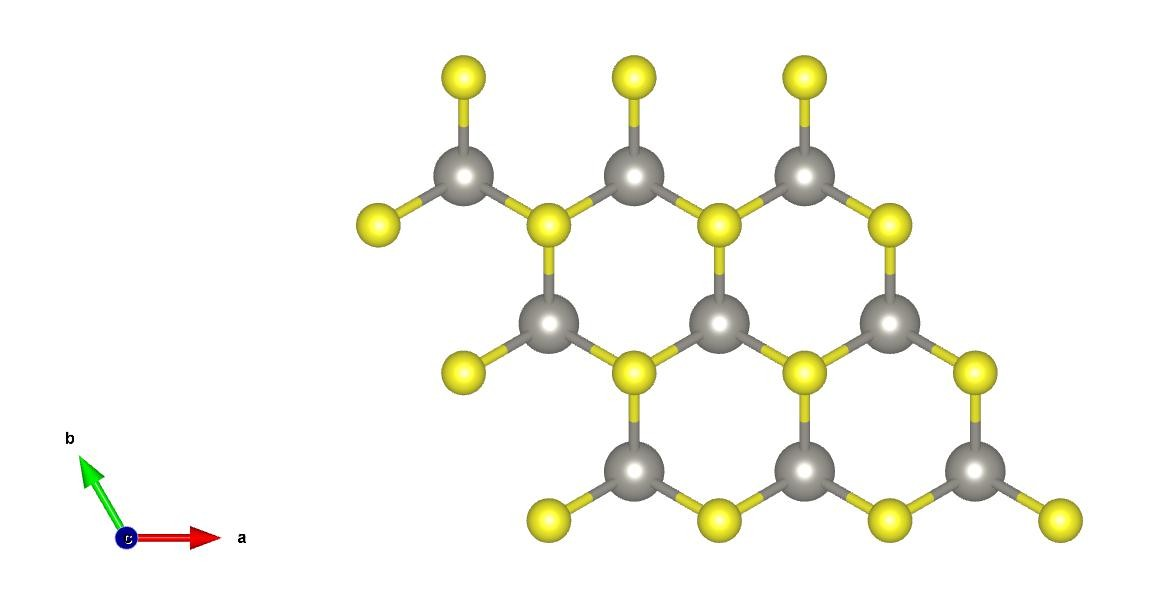
\includegraphics[width=1.0\textwidth]{img/TMDs_structure.jpg} 
\caption{TMDs 晶格結構俯視圖。灰色球體為 $\text{W}$，黃色球體為 $\text{S}$。} 
\label{fig:tmds_structure_a} 
\end{figure} 

\begin{figure}[H] 
\centering 
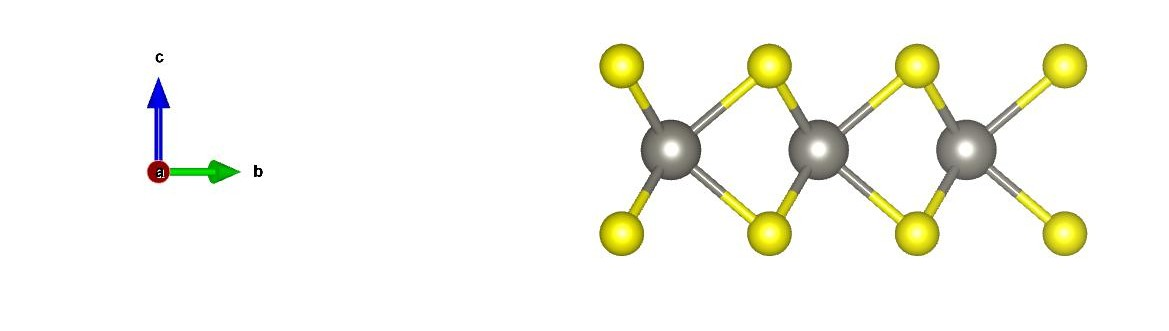
\includegraphics[width=1.0\textwidth]{img/TMDs_structure_2.jpg} 
\caption{TMDs 晶格結構側視圖。灰色球體為 $\text{W}$，黃色球體為 $\text{S}$。} 
\label{fig:tmds_structure_b} 
\end{figure}

\subsubsection*{能帶結構、自旋軌道耦合與激子物理}

在能帶結構方面，過渡金屬原子 (尤其是 W 基材料) 的強自旋軌道耦合 (Spin-Orbit Coupling, SOC) 在 $K$ 點的價帶頂造成顯著的自旋分裂，形成能量不同的上、下兩個自旋子帶。此分裂量在 W 基材料 (WS$_2$、WSe$_2$) 中高達 400–460 meV，在 Mo 基材料 (MoS$_2$、MoSe$_2$) 中約為 140–160 meV。由於時間反演對稱性的限制，$K$ 與 $K'$ 谷的自旋分裂方向恰好相反，形成自旋–谷鎖定效應 (Spin-Valley Locking)：在 $K$ 谷，自旋向上的電子佔據較高的價帶子帶；在 $K'$ 谷，自旋向下的電子佔據對應位置 \cite{xiao2012coupled}。


\begin{figure}[H] 
\centering 
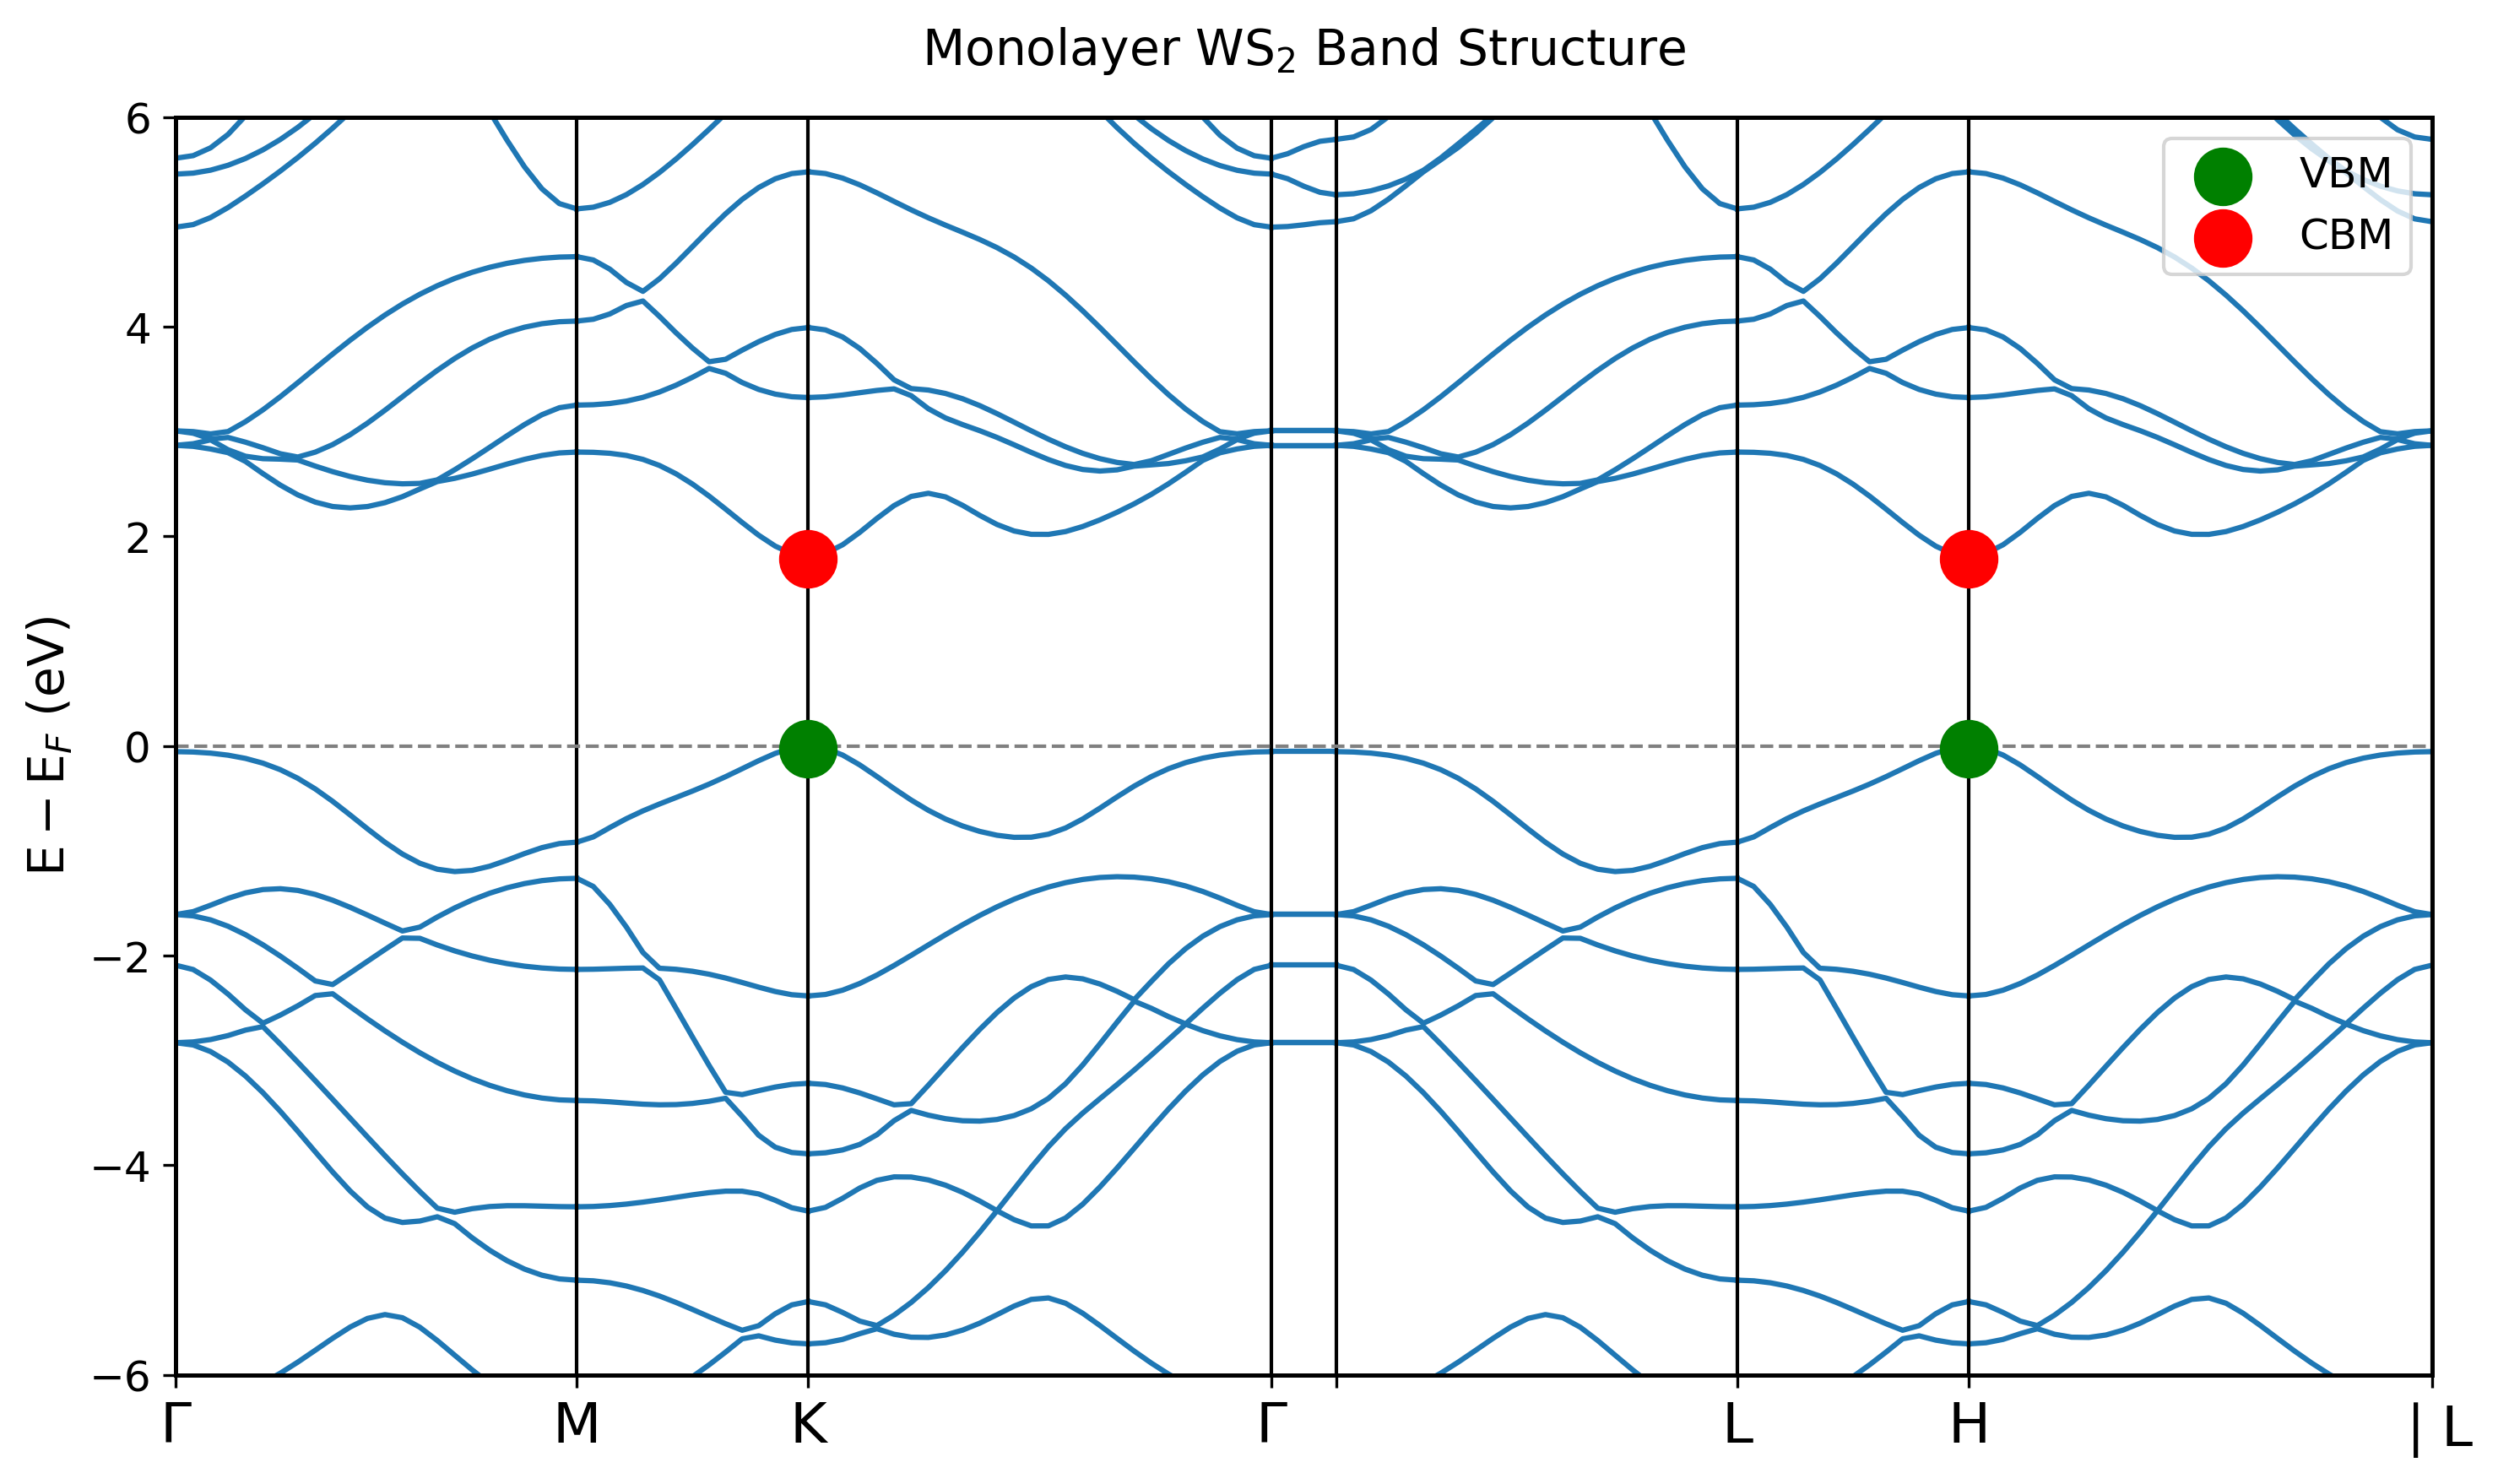
\includegraphics[width=1.0\textwidth]{img/WS2_8points_markers.png} 
\caption{單層 $\text{WS}_2$ 能帶結構圖。$K$ 與 $K'$ ($H$) 谷處的垂直線代表直接能隙位置。綠點為價帶頂 (VBM)，紅點為導帶底 (CBM)，兩者的能量差即為形成 A 激子所需的最小能量。} 
\label{fig:tmds_structure_c} 
\end{figure}

在此能帶結構之上，光學激發所產生的電子-電洞對因強烈的庫倫吸引力而束縛在一起，形成激子 (Exciton) –– 一種由電子與電洞組成的準粒子。相較於三維塊材半導體，二維材料中的庫倫交互作用因介電屏蔽大幅降低而顯著增強，使激子束縛能高達 0.3–0.5 eV，遠大於室溫熱能 ($k_BT \approx 26\text{ meV}$)，確保激子在室溫下依然穩定存在，成為 TMDs 光學響應的主體 \cite{wang2018colloquium}。

依據躍遷所涉及的價帶子帶，可定義兩類激子。A 激子 (A Exciton) 由導帶底至較高自旋子帶 (較靠近費米能的 VB 上子帶) 的躍遷所形成，發光能量較低；B 激子 (B Exciton) 則由導帶底至較低自旋子帶 (VB 下子帶) 的躍遷所形成，兩者發光能量之差即為自旋軌道分裂量 $\Delta_{\text{SOC}}$。在本論文後續的文獻回顧與模擬討論中，所涉及的谷選擇性發光訊號均以 A 激子躍遷為主體。

\subsubsection*{谷選擇定則的量子力學推導}

谷選擇定則的物理根源，可從電偶極光學矩陣元素的對稱性出發進行嚴格推導。在 $D_{3h}$ 點群的約束下，$K$ 與 $K'$ 谷的導帶底 Bloch 態主要由過渡金屬原子的 $d_{z^2}$ 軌道貢獻 (磁量子數 $m = 0$)；而 $K$ 谷與 $K'$ 谷的價帶頂 Bloch 態分別由 $d_{x^2-y^2}$ 與 $d_{xy}$ 軌道組合為 $d_{\pm 2} \equiv  (d_{x^2-y^2} \pm id_{xy})/\sqrt{2}$，等效磁量子數為 $m = \pm 2$，其中正負號分別對應谷指標 $\tau = \pm 1$ ($K$ 谷與 $K'$ 谷)。
光學躍遷的電偶極矩陣元素可以表示為：
\begin{align}
\mathbf{P}_\tau = \langle u_{c,\tau\mathbf{K}} | \hat{\mathbf{p}} | u_{v,\tau\mathbf{K}} \rangle
\end{align}
定義對應左右旋圓偏振光的動量算符 $\hat{p}_\pm = \hat{p}_x \pm i\hat{p}_y$ (分別對應光子角動量 $\pm\hbar$)。由角動量守恆，利用 $D_{3h}$ 不可約表示的選擇定則，可嚴格驗證：
\begin{align}
|\langle u_{c,\mathbf{K}} | \hat{p}_+ | u_{v,\mathbf{K}} \rangle|^2 &\neq 0, \quad |\langle u_{c,\mathbf{K}} | \hat{p}_- | u_{v,\mathbf{K}} \rangle|^2 = 0 \\
|\langle u_{c,\mathbf{K}'} | \hat{p}_+ | u_{v,\mathbf{K}'} \rangle|^2 &= 0, \quad |\langle u_{c,\mathbf{K}'} | \hat{p}_- | u_{v,\mathbf{K}'} \rangle|^2 \neq 0
\end{align}
此嚴格的選擇定則表明：本研究設定下，$\text{K}$ 谷由左旋圓偏振光 ($\text{LCP}, \sigma^-$) 選擇性激發，而 $\text{K}'$ 谷則由右旋圓偏振光 ($\text{RCP}, \sigma^+$) 選擇性激發，展現了光子自旋角動量 (SAM) 與電子谷自由度之間的鎖定關係 \cite{xiao2012coupled}。

在實驗操作上，透過給定螺旋性的圓偏振光對單層 TMDs 進行光學激發，可選擇性地在單一谷中激發電子-電洞對，打破兩谷間的載子平衡，實現動態的谷極化。當這些極化的谷激子發生輻射復合時，其光致發光會繼承激發光的偏振特性，$K$ 谷與 $K'$ 谷的激子發射分別產生高純度的 $\sigma^-$ 與 $\sigma^+$ 圓偏振光。

谷極化發射的純度通常以圓偏振度 (degree of circular polarization, $Pc$) 來量化，定義為左右旋偏振發光強度的差值與總和之比：
\begin{align}
Pc = \frac{I (\sigma^+) - I (\sigma^-)}{I (\sigma^+) + I (\sigma^-)}
\end{align}
由於光子的圓偏振特性在物理本質上即對應於光子的 SAM，單層 TMDs 的谷極化輻射使其成為極具潛力的單光子源與操控光子 SAM 的理想載體 \cite{gong2018nanoscale}。然而，為了進一步提升光學資訊的乘載與處理能力，如何將此固有的谷自由度 (SAM) 進一步轉換為光子的 OAM，成為近代自旋光子學的研究核心。

在超穎表面與全介電質谷光子晶體技術的發展下，透過特殊設計的微奈米結構，已被證實能夠調控並展現具備谷對比特性的 OAM，進而實現谷手性的單向激發 \cite{chen2017valley}。這為晶片整合的量子資訊處理與多維度光學調控提供了全新且關鍵的解決方案。

\subsection{Spin-Orbit Interaction and SAM-to-OAM Conversion}

光子的自旋軌道交互作用  (Spin-Orbit Interaction, SOI) 描述光子的 SAM  (偏振狀態) 與空間 OAM  (波前幾何結構) 之間的相互耦合機制。在不同的光學系統中，SOI 可透過不同的幾何機制被引發：在強聚焦光學系統中，波前的急劇彎曲引發自發性的 SAM 到 OAM 轉換；而在平面奈米光子學中，空間非均勻的幾何相位調控則提供了晶片整合的 SOI 實現路徑。以下分別闡述這兩種機制。

\subsubsection*{強聚焦系統中的自旋軌道交互作用}

當光學系統進入非近軸範疇，SAM 與 OAM 將不再獨立。在強聚焦系統中，光線會以極大的角度向中心匯聚，使得波前發生劇烈彎曲，並在焦點附近形成極具空間不均勻性的橫向電場分佈。此時，其橫向空間梯度 ($\partial E_x/\partial x$ 與 $\partial E_y/\partial y$) 將會大幅增加，為了滿足馬克士威方程式中的高斯定律：
\begin{align}
\nabla \cdot \mathbf{E} = \frac{\partial E_x}{\partial x} + \frac{\partial E_y}{\partial y} + \frac{\partial E_z}{\partial z} = 0
\end{align}
系統必然會產生顯著的縱向電場分量 $E_z$，其振幅大小與橫向分量 $E_x, E_y$ 相當，在數學計算與物理效應上皆不可忽略。這種由幾何邊界與波前結構驅動的場分量耦合轉換，便是引發光學自旋軌道交互作用的核心機制。

為了具體量化此物理現象，以攜帶 SAM  ($s = \pm 1$) 的圓偏振高斯光束經過高數值孔徑透鏡強聚焦為例。當入射光為左旋圓偏振 (LCP, $s = +1$) 時，其入射電場可表示為：
\begin{align}
\mathbf{E}_{in} = \mathbf{E}_{0}  (r,z)  (\hat{x} + is\hat{y})e^{ikz}
\end{align}
若將公式轉換至柱座標系，則可展開為：
\begin{align}
\mathbf{E}_{\text{in}} \propto  (\hat{x} + is\hat{y}) =  (\cos\phi \hat{\rho} - \sin\phi \hat{\phi}) + is (\sin\phi \hat{\rho} + \cos\phi \hat{\phi})
\end{align}
當光線經透鏡聚焦傾斜 $\theta$ 時，由於方位角分量 ($\hat{\phi}$ 項) 始終與 $z$ 軸垂直，只有徑向分量 ($\hat{\rho}$ 項) 會投影到 $z$ 軸。單獨提取 $\hat{\rho}$ 前面的係數，其幾何投影關係為：
\begin{align}
\text{Projection to } z \propto \cos\phi + is\sin\phi = e^{is\phi}
\end{align}
在 Richards-Wolf 高 NA 聚焦理論中，焦點總電場是透過對透鏡孔徑面上的平面波進行二維角譜積分得到。計算縱向電場分量 $E_z$ 的孔徑面方位角環向積分為：
\begin{align}
E_z \propto \int_0^{2\pi} e^{is\phi_p} e^{ik\rho\cos (\phi_p - \phi)} d\phi_p = e^{is\phi} \int_0^{2\pi} e^{is\alpha} e^{ik\rho\cos\alpha} d\alpha
\end{align}
方位角相位 $e^{is\phi}$ 被提到積分符號外面，右側積分項正比於一階第一類貝索函數 $J_1 (k\rho\sin\theta)$。因此，焦平面 ($z=0$) 附近的縱向電場分量可嚴格推導為：
\begin{align}
E_{z} (\rho, \phi, z) = -iAe^{is\phi}I_{1} (\rho,z), \quad I_1 (\rho, z) = \int_0^\alpha \cos^{1/2}\theta \sin^2\theta P (\theta) J_1 (k\rho\sin\theta) e^{ikz\cos\theta} d\theta
\end{align}
其中 $A$ 為振幅常數，$P (\theta)$ 為切趾函數，$\alpha$ 為最大聚焦半角。$E_z$ 中自發性地衍生出拓撲荷 $\ell = s = +1$ 的螺旋相位因子 $e^{is\phi}$，即原本純粹由偏振狀態決定的 SAM，在強聚焦的幾何邊界約束下，部分能量轉換成帶有螺旋波前的 OAM，闡明了強聚焦系統中 SAM 到 OAM 轉換的物理機制。

\subsubsection*{幾何相位 (Pancharatnam–Berry Phase)與平面奈米光子學中的 SOI}

上述強聚焦 Richards–Wolf 推導揭示，SAM 到 OAM 的轉換本質上源自於空間相位梯度與偏振態的幾何耦合。在平面奈米光子學元件的設計框架中，實現此類 SOI 轉換並不依賴大數值孔徑透鏡系統，而是透過另一種更適合晶片整合的機制––幾何 (Pancharatnam–Berry)相位––來完成。

幾何相位的物理根源最早由 Pancharatnam 於 1956 年在光學干涉的情境中提出 \cite{pancharatnam1956generalized}，後由 Berry 於 1984 年推廣為量子力學的普遍原理 \cite{berry1984quantal}：當一個量子態在參數空間中沿閉合路徑絕熱演化回到初態時，除積累動力學相位外，還會額外獲得一個僅由演化路徑幾何形狀決定的相位。在光學偏振的情境中，偏振態可以用龐加萊球 (Poincaré Sphere)上的一點表示：北極對應右旋圓偏振 ($\sigma^+$)，南極對應左旋圓偏振 ($\sigma^-$)，赤道上各點對應不同方位角的線偏振態。當偏振態在 Poincaré 球面上沿一閉合路徑演化時，所積累的 Pancharatnam–Berry 相位 (PB 相位) 等於該路徑在球面上所圍固體角 $\Omega_\text{solid}$ 之半：
\begin{align}
\Phi_{\text{PB}} = \frac{\Omega_\text{solid}}{2}
\end{align}
對於一個局部雙折射奈米天線，當其快軸旋轉角度 $\theta$ 時，通過後的交叉極化分量在 Poincaré 球上的演化路徑從 $\sigma^+$ 出發，經由赤道上旋轉 $2\theta$ 的線偏振中間態到達 $\sigma^-$，整個閉合路徑所圍固體角為 $4\theta$，因此 PB 相位為：
\begin{align}
\Phi_{\text{PB}} = \frac{4\theta}{2} = 2\theta
\end{align}
此結果表明，PB 相位的符號與大小完全由天線的空間旋轉角度 $\theta$ 決定，而與波長無關，賦予幾何相位超穎表面優越的寬頻特性。

基於上述 PB 相位的物理根源，考慮一局部雙折射奈米結構 (如超穎表面的天線單元)，假設其快軸相對於參考軸的局部方位角為 $\theta (\phi)$，其中 $\phi$ 為方位角。當一圓偏振光 ($\sigma_z = \pm 1$) 入射該結構時，穿透或反射的光場除了包含保持原偏振的共極化分量外，還會產生一個手性相反的交叉極化分量。該交叉極化分量會額外獲得一個與結構空間方位直接相關的幾何相位移：
\begin{align}
\Omega = \mp 2\theta (\phi)
\end{align}
若進一步將奈米結構的空間方位設計為隨方位角呈線性變化，即滿足關係式 $\theta (\phi) = q\phi$ (其中 $q$ 為半整數或整數)，則入射的圓偏振光在通過該結構後，其交叉極化分量所附加的幾何相位將演變為 $\exp (\mp i 2q\phi)$。根據 \ref{ssec:oam of light} 對螺旋相位的定義，此方位角相關的相位分佈正對應於拓撲荷為 $\ell = \mp 2q$ 的 OAM 模態。

幾何相位超穎表面為實現 SAM 到 OAM 轉換提供了最具代表性的有效平台之一。然而更廣義而言，光子的 SOI 可透過在空間中非均勻分佈的光學響應進行任意調控。藉由打破傳統單元結構旋轉的局部幾何相位限制，可在更廣義的二維非均勻介質中，自由操控空間相位梯度，進而實現具備客製化 OAM 狀態的任意結構光場。這為利用新型非直覺光學結構調控波前、產生高純度 OAM 模態奠定了理論基礎。

\subsection{Inverse Design and Topology Optimization}

在奈米光學元件的傳統設計方法中，通常採用正向設計，即依賴物理直覺或既有的經驗幾何圖形 (如圓柱、矩形天線) 進行有限的參數掃描。然而，這種方法強烈受限於人類的幾何直覺，且僅能調控極少數的自由度，難以應對非直覺、多功能或極端非對稱的高難度光場調控需求。

為了突破傳統設計的瓶頸，反向設計方法應運而生。反向設計將光學元件設計轉化為一個嚴謹的數學最佳化問題：首先定義一個具體描述目標性能的目標函數 (Figure of Merit, FOM)，再從目標結果出發，反向尋找最優的空間介電常數分佈。

在面對高維度設計空間時，結合伴隨變量法的拓樸最佳化展現出極大的數值優勢。伴隨變量法僅需進行兩次全波電磁模擬 (正向模擬與反向伴隨模擬)，即可高效計算出目標函數對於成千上萬個空間網格的精確梯度。藉由梯度下降等最佳化演算法，拓樸最佳化能在奈米尺度下自由調整物質的幾何邊界與拓撲結構，從而在龐大的參數空間中自動演化出超越傳統直覺的高性能光學結構，為實現理想光學結構提供了強大的核心數值方法支撐。

\section{State of Related Research}

\subsection{Metasurface-based OAM Generation}

模態純度已成為最重要的指標之一，用於評估 OAM 產生器的性能。

早期的 OAM 超穎表面多採用電漿子金屬奈米天線陣列，例如 Karimi 等人於2014年利用空間漸變的超薄 L 型金奈米結構，在可見光波段實現了基於幾何相位的 OAM 渦旋產生器 \cite{karimi2014generating}。然而，純粹依賴離散奈米天線的相位調控易產生相位雜訊，激發的高階徑向模態常使出射光束產生多重同心圓環的非理想光場分佈 \cite{karimi2014generating}。為了解決上述缺陷並提升模態純度，Guo 等人提出將幾何相位與電漿子延遲相位結合於連續形狀的超穎表面中，成功將拓樸荷 $\ell = 2$ 的光學渦旋純度從離散結構的 $64\%$ 提升至 $90\%$ 以上 \cite{guo2016merging}，特別強調了相位分佈的幾何連續性對於抑制模態串擾和提高 OAM 純度方面的重要性。

為突破電漿子材料的損耗限制，近年的研究主流轉向低損耗的介電質平面光學與全介電質超穎表面。針對傳統 OAM 光環尺寸隨拓撲荷增加而發散的應用瓶頸，Liu 等人於2017年提出利用超薄的石英玻璃平面相位元件，實驗上成功產生了光環尺寸獨立於拓撲荷的完美渦旋光束，大幅縮小了傳統光學系統的體積 \cite{liu2017generation}。這些高純度的腔外調控技術進一步促成了光電系統的發展，例如 Bi 等人於2018年與 Tan 等人於2019年分別在毫米波段與自由空間光通訊中實現了寬頻與多工傳輸 \cite{bi2018metasurface, tan2019free}。另一方面，如何在複雜的多工影像重建中保持 OAM 的空間相位特徵並抑制像素間的模態串擾，Ren 等人於2019年提出了空間頻率採樣與相位補償技術 \cite{ren2019metasurface}，該研究揭示了遠場干涉對 OAM 螺旋波前的破壞機制，並藉由傅立葉空間離散採樣與基態濾波技術，成功抑制了重建像素間的螺旋波前干涉與模態串擾，為高容量空間光學多工系統奠定基礎。

儘管上述腔外系統取得諸多進展，其純度依然受限於元件加工精度與傳播繞射。為突破此純度極限，Sroor 等人於 2020 年首創將二氧化鈦全介電質超穎表面整合至雷射共振腔內\cite{sroor2020high}。該研究證實，雷射腔內的繞射、共振與增益輔助濾波機制能自然過濾掉不需要的徑向散射模態，即使在 $\ell=100$ 的極高階 OAM 狀態下，依然能有效抑制高階徑向模態，將 $p=0$ 的目標模態純度維持在近 $90\%$ 。 在此技術發展的基礎上，為了進一步提升設計自由度，Zhou 等人於 2021 年利用二氧化鈦全介電質幾何超穎表面，成功生成了光環半徑獨立於拓撲荷變化的完美渦旋光束，展示了能在單一元件上，同時獨立調控光束尺寸與橢圓率等多維度特徵的能力 \cite{zhou2021generation}。

儘管現有的 OAM 超穎表面已展現卓越性能，但現行元件主要仍依賴基於單元結構的正向設計方法，即透過排列特定形狀的奈米天線來實現相位調控。預先定義的幾何模板嚴格限制了此類設計的自由度。雖然高純度的 OAM 光束已在上述文獻中被個別驗證，但其元件表現依然強烈依賴這些特定的原子幾何與相位工程策略，難以在多目標光場調控中達到全局最佳化。

\begin{table}[h]
\centering
\caption{超穎表面 OAM 產生技術發展年表}
\label{tab:timeline_oam}
\small
\begin{tabular}{c p{11cm}}
\toprule
\textbf{年份} & \textbf{文獻重點} \\
\midrule
2014 & 以漸變 L 型金奈米結構陣列實現幾何相位 OAM 渦旋產生器，驗證電漿子超穎表面生成渦旋光 \cite{karimi2014generating} \\
2016 & 幾何相位與延遲相位結合，連續形超穎表面將 OAM 模態純度從 64\% 提升至 90\% 以上 \cite{guo2016merging} \\
2017 & 石英玻璃平面相位元件產生完美渦旋光束，光環尺寸獨立於拓撲荷大小 \cite{liu2017generation} \\
2018 & 超穎表面實現毫米波 OAM 多工寬頻傳輸 \cite{bi2018metasurface} \\
2019 & 超穎表面實現自由空間光通訊 OAM 多工傳輸 \cite{tan2019free} \\
2019 & 空間頻率採樣與相位補償技術抑制 OAM 多工重建中的螺旋波前干涉 \cite{ren2019metasurface} \\
2020 & TiO$_2$ 超穎表面整合至雷射共振腔，$\ell=100$ 高階 OAM 模態純度仍維持近 90\% \cite{sroor2020high} \\
2021 & TiO$_2$ 幾何超穎表面生成完美渦旋光束，在單一元件上獨立調控光束尺寸與橢圓率 \cite{zhou2021generation} \\
\bottomrule
\end{tabular}
\end{table}

\subsection{Valley-controlled Chiral Photonics}

TMDs 因空間反轉對稱性破缺與強 SOC 的協同作用，催生了獨特的自旋能谷鎖定效應 \cite{xiao2012coupled}。圓偏振光可選擇性調控電子的谷自由度，並能透過偏振解析光致發光光譜進行高效的光學初始化與檢測 \cite{mak2012control, zeng2012valley, schaibley2016valleytronics}。

然而，單層 TMDs 中的激子壽命與谷極化壽命通常極短 (僅約數個皮秒)，這極大地限制了谷資訊的邏輯運算與在晶片上的長距離空間傳輸 \cite{schaibley2016valleytronics, gong2018nanoscale}。為了克服此關鍵退相干與損耗瓶頸，學界主要沿著兩條互補的技術路徑展開探索：一是聚焦於利用微奈米光學共振腔的 Purcell 效應提高局域光子態密度，以加速單層 TMDs 的激子自發輻射速率並提升其發光效率 \cite{mak2016photonics, gan2013controlling}；然而，傳統微腔往往缺乏手性選擇性，無法主動維持或操縱激子的谷極化特徵 \cite{mak2016photonics}。另一條更具針對性的路徑，則是利用二維材料固有的谷選擇性圓偏振光學躍遷定則 \cite{xiao2012coupled}，將其與具備光學自旋動量鎖定特性的一維導波結構進行近場耦合，從而建立奈米尺度下的手性能谷光子介面，實現谷極化資訊的定向提取與晶片上傳輸。

其中最具代表性的是Gong 等人於2018年的研究 \cite{gong2018nanoscale}。在具體實作上，該研究將少層 $\text{WS}_2$ 與單根銀奈米線近場耦合。利用表面電漿子極化子波導模態因光學 SOC 所攜帶的本徵橫向光學自旋角動量，達成光學自旋動量鎖定，從而將少層材料中谷選擇性激發的近場圓偏振偶極發光，高效率地轉化為該模態的單向定向傳輸，其定向耦合效率高達 $90 \pm 1\%$。此工作成功建立了奈米尺度下的手性谷-光子介面，也證實了在室溫下進行谷資訊面內傳輸的可行性。

儘管金屬導波結構能藉由電磁場的強局域化實現極高耦合效率，但金屬本徵的高歐姆損耗卻嚴重限制了谷資訊的實際傳輸距離。為了解決此損耗瓶頸，後續研究開始探索TMDs與低損耗的全介電質、高折射率奈米波導或光子晶體波導進行耦合。在這一領域，將二維材料與低損耗、高折射率全介電質微腔整合以調控激子發光的實驗先驅，首推 Gan 等人於 2013 年的研究 ，以及隨後 Wu 等人於 2014 年的研究 \cite{gan2013controlling, Wu2014control}。在這些工作中，學者打破了傳統將發光介質嵌入光子晶體內部的結構限制，首次將單層二維材料轉移至預先製備的 GaP (磷化鎵) 光子晶體微腔表面；這不僅完美避免了蝕刻製程對二維材料激子特性的破壞，更在實驗上觀測到自發輻射速率的有效調控 \cite{gan2013controlling, Wu2014control}。

近年來的研究進一步朝向更小模態體積與超穎表面調控的方向發展。例如，Sortino 等人於 2019 年的研究採用了GaP 奈米天線，與單層及雙層 $\text{WSe}_2​$ 進行近場耦合 \cite{sortino2019enhanced}。該研究利用極小模態體積的低損耗 $\text{GaP}$ 共振腔，在完全避免金屬非輻射與歐姆損耗的同時，實現了高達 $10^4$ 以上的光致發光強度增強，並透過 Purcell 效應使激子輻射衰期縮短至系統偵測極限。這一系列從光子晶體微腔到介電質奈米天線的進展證實了，全介電質 GaP 奈米結構能有效克服金屬的損耗瓶頸，成為高效操控二維激子發光的優異平台。

除了在晶片表面進行面內的定向波導，如何主動調控谷極化發光在自由空間中的三維輻射行為，亦成為另一關鍵課題。透過在 TMDs 表面建構人工設計的全介電質手性超穎表面，學者得以在避免歐姆損耗的前提下實現面外波前調控，進而發展出低損耗的手性超穎表面、谷選擇性全息投影以及攜帶 OAM 的渦旋光束發射。

在面外三維空間調控的實驗中，如何打破系統的面外對稱性以高效提取特定手性的谷極化光子是核心挑戰。為此，Rong 等人於 2020 年的研究取得了突破性進展 \cite{rong2020photonic}。研究使用多晶矽介電質材料以避免金屬損耗，並激發了光子拉希巴 (Rashba) 效應，成功將單層 $\text{WSe}_2$ 的內稟谷自旋轉化為向自由空間特定方向輻射的自旋鎖定窄光束，達成了極高指向性的面外波束成型。

隨著奈米光學與二維材料光電元件的快速演進，研究視野已從傳統的面內定向導波，跨越至如何高效提取並調控自由空間的面外手性輻射。然而，在建構主動式手性光源元件時，研究面臨著根本性的物理挑戰：直接能隙的單層 TMDs 雖具有極高的激子輻射效率與內稟谷自旋選擇性，但其原子級的超薄厚度 (約 $0.7\text{ nm}$) 卻限制了局域電磁場的交互作用與相位調控能力；相反地，雖然多層材料或直接對 TMDs 進行亞波長圖案化的無源器件能提供足夠的幾何相位調控，但多層 TMDs 因轉變為間接能隙，其發光效率呈指數級衰減。因此，將高發光效率的單層 TMD 活性層，與低損耗、高折射率介電質超穎表面進行混合整合，已成為構建二維手性光源與雷射晶片的最佳技術路徑。

在這一技術路徑上，近期的研究取得了里程碑式的進展。例如，Rong 等人於 2023 年的研究將單層 $\text{WS}_2$ 轉移至 $\text{Si}_3\text{N}_4$ Kagome 光子晶體晶格表面，藉由打破空間反轉對稱性激發光子 Rashba 效應，在室溫下成功實現了高相干性的自旋-谷鎖定單層雷射 \cite{rong2023spin}。隨後，Pan 等人於 2025 年的研究則利用矽手性超穎表面激發高活性、強手性近場增強的非局域準連續域束縛態，在室溫下將單層 $\text{MoSe}_2$ 的谷選擇性發光圓偏振極化度提升至新高 \cite{pan2025room}。

儘管這些基於高品質因子腔體的混合元件在提升手性提取效率與激子輻射速率上表現優異，但目前的設計仍存在顯著的技術瓶頸。現有元件多依賴於週期性、高度對稱的常規晶格幾何 (如 Kagome 晶格或切角正方形陣列) ，這使得其遠場波前調控能力通常被局限於簡單的定向偏折窄光束或多對稱輻射點。在無需外部偏振濾光片的前提下，如何直接對單層 TMD 激子的自發輻射進行高自由度的複雜波前塑形 (例如直接產生攜帶 OAM 、高模態純度的渦旋光束或 LG 模態) ，並同時維持極高的谷極化選擇性，依然是當前自旋-谷光電子晶片面臨的核心瓶頸。

\begin{table}[h]
\centering
\caption{谷手性光子學研究發展年表}
\label{tab:timeline_valley}
\small
\begin{tabular}{c p{11cm}}
\toprule
\textbf{年份} & \textbf{文獻重點} \\
\midrule
2012 & 理論預測單層 TMDs 因反轉對稱破缺形成自旋能谷鎖定，建立谷選擇性光學躍遷定則 \cite{xiao2012coupled} \\
2012 & 實驗驗證 MoS$_2$ 谷極化光學初始化，以圓偏振光選擇性激發單一能谷 \cite{mak2012control} \\
2012 & 確認 WSe$_2$ 谷選擇性圓偏振光致發光，奠定谷電子學實驗基礎 \cite{zeng2012valley} \\
2013 & 首次將單層二維材料轉移至 GaP 光子晶體微腔表面，觀測自發輻射速率調控 \cite{gan2013controlling} \\
2014 & GaP 光子晶體微腔調控單層 TMD 激子自發輻射速率，驗證介電質腔與二維材料整合 \cite{Wu2014control} \\
2016 & 系統回顧谷電子學進展，指出皮秒激子壽命限制谷資訊在晶片上的長距離傳輸 \cite{schaibley2016valleytronics} \\
2018 & WS$_2$ 與銀奈米線近場耦合，谷選擇性定向耦合效率達 $90\pm1$\% \cite{gong2018nanoscale} \\
2019 & GaP 奈米天線與 WSe$_2$ 近場耦合，PL 增強 $10^4$ 倍並透過 Purcell 效應縮短輻射衰期 \cite{sortino2019enhanced} \\
2020 & 多晶矽超穎表面激發光子 Rashba 效應，將 WSe$_2$ 谷自旋轉化為定向自旋鎖定窄光束 \cite{rong2020photonic} \\
2023 & 單層 WS$_2$ 結合 Si$_3$N$_4$ Kagome 光子晶體，室溫實現自旋-谷鎖定相干雷射 \cite{rong2023spin} \\
2025 & 矽手性超穎表面激發準 BIC 強手性近場，室溫大幅提升 MoSe$_2$ 谷選擇性圓偏振度 \cite{pan2025room} \\
\bottomrule
\end{tabular}
\end{table}

\subsection{Existing Valley-to-OAM Conversion Platforms}

關於現存的能谷與 OAM 轉換技術，近期的研究主要依賴能谷軌道耦合效應或特定的光子共振態來實現。

部分學者利用應力陷阱在單層半導體中捕捉層內激子，藉由電子-電洞庫倫交換作用所介導的激子質心動量與能谷自由度的本徵耦合，在奈米尺度下實現了光子 SAM 與 OAM 鎖定的單光子發射 \cite{zhang2023single}。此外，亦有研究將非中心對稱的 TMDs 圖案化為光子晶體超穎表面，使其與連續體束縛態 (Bound States in the Continuum, BIC) 發生強耦合形成激子極化子\cite{li2023valley}。在此物理圖像中，BIC 的拓撲荷 $q$ 被定義為動量空間中偏振主軸角度 $\phi(k)$ 沿閉合路徑 $C$ 的積分，其關係式可表示為 $q=\frac{1}{2\pi}\oint_{C}dk\cdot\nabla_{k}\phi(k)$。此拓撲特性賦予了遠場輻射的偏振渦旋結構，藉由自旋-谷鎖定選擇定則，成功將 TMDs 的能谷自由度與光子 OAM 的拓撲荷直接連結 \cite{li2023valley}。此種由能谷物理主導的手性調控，近年亦被成功推廣至人工拓撲光子平台。同時，結合克庫勒調變的自製狄拉克渦旋微腔，亦被證實能透過能谷間耦合與自旋能谷鎖定的協同機制，自發輻射出具備高度自旋軌道角動量鎖定 (Spin-orbit angular momentum locking) 的特定 OAM 渦旋光束 \cite{li2026unveiling}。

儘管上述研究成功實現了能谷資訊與光波 OAM 的結合，這些技術路線仍面臨純度受限與調控彈性不足的雙重挑戰。應力陷阱方法雖能產生具備 OAM 的單光子，但應力分佈的隨機性與周遭環境干擾容易導致出射光純度下降；而結合 BIC 或克庫勒調變的超穎表面，其生成的 OAM 階數高度依賴於固定的晶格對稱性 (如四重旋轉對稱)，難以在單一元件上進行動態且彈性的高階模態切換。更為關鍵的是，目前學界仍缺乏一個能直接將谷極化高純度轉換為特定 LG 模態的直接轉換平台。

因此，如何突破既有平台受限於特定共振機制與晶格對稱性的限制，建立具有更高設計自由度的 Valley-to-OAM 轉換架構，已成為目前的重要研究方向。

\begin{table}[h]
\centering
\caption{現有能谷–OAM 轉換平台研究年表}
\label{tab:timeline_v2oam}
\small
\begin{tabular}{c p{11cm}}
\toprule
\textbf{年份} & \textbf{文獻重點} \\
\midrule
2023 & 應力陷阱捕捉層內激子，庫倫交換作用介導 SAM–OAM 鎖定的單光子發射 \cite{zhang2023single} \\
2023 & TMDs 光子晶體超穎表面與 BIC 強耦合，谷自由度與光子 OAM 拓撲荷直接連結 \cite{li2023valley} \\
2026 & 克庫勒調變狄拉克渦旋微腔透過自旋能谷鎖定機制，自發輻射高純度 OAM 渦旋光束 \cite{li2026unveiling} \\
\bottomrule
\end{tabular}
\end{table}

\subsection{Inverse-designed Nanophotonic Devices}

傳統的奈米光子元件設計高度依賴物理直覺與有限的幾何參數掃描，面臨結構複雜化帶來的瓶頸。為突破限制，自動化尋找光學結構的反向設計近年成為奈米光子領域的核心技術 \cite{jensen2011topology, molesky2018inverse}。其中，拓撲最佳化賦予設計空間最大的自由度；與傳統以單元結構為基礎的正向設計不同，拓撲最佳化不需預先假設結構形狀，而是在連續設計空間中直接搜尋最佳介電質分布，從而探索出非直觀的結構 \cite{jensen2011topology}。因此，這種方法特別適合需要同時最佳化振幅、相位、偏振與模態純度等多重目標的複雜波前設計。為在龐大自由度中高效收斂，伴隨變量法至關重要，其僅需前向與伴隨兩次電磁場模擬即可高效計算出目標函數對所有幾何參數的梯度，極大幅降低了計算成本，使複雜光子元件的自動化設計成為可能。

在超穎表面的研究中，反向設計展現了強大的多功能整合與光場調控能力。近期成果已廣泛涵蓋高效率非對稱光束偏轉 \cite{li2022empowering}、大數值孔徑消色差超透鏡聚焦 \cite{choi2025roll}、全斯托克斯偏振成像偵測 \cite{wang2024non} 及多維多通道複用全像顯示 \cite{yin2024multi}。這些自由曲面元件透過拓撲最佳化達到了傳統幾何結構無法企及的傳輸效率與功能密度，證明了反向設計在操縱複雜光場上的成熟度與優勢。

然而，綜觀現有的反向設計超穎表面研究，其核心機制主要聚焦於空間中光波之振幅、相位與偏振的基本調控 \cite{molesky2018inverse, li2022empowering}。

相較之下，將反向設計應用於二維材料的谷發射器調控仍處於起步階段。現有 TMDs 的谷發射調控多依賴傳統物理直覺設計的電漿子或奈米線結構 \cite{mak2012control, deng2021plasmonic}。雖然已有研究將反向設計與單層 TMDs 結合以進行腔耦合或暗激子偵測 \cite{gelly2023inverse}，但針對特定谷手性的高自由度發射調控仍極為稀缺。更具挑戰性的是，目前極少有研究探討如何將特定谷自由度的手性圓偏振發光，直接轉換為攜帶 OAM 的 LG 光束。

儘管矽晶片已能實現高效的反向設計 OAM 發射器 \cite{white2023inverse}，目前還未有同時進行動量匹配、手性選擇與空間模態變換的谷選擇性反向設計發射器。此一研究缺口正是本文所欲探討與解決的核心課題。

\begin{table}[h]
\centering
\caption{反向設計奈米光子元件研究發展年表}
\label{tab:timeline_inverse}
\small
\begin{tabular}{c p{11cm}}
\toprule
\textbf{年份} & \textbf{文獻重點} \\
\midrule
2011 & 提出拓撲最佳化框架，以梯度法在奈米光子設計空間中自動搜尋最佳介電分布 \cite{jensen2011topology} \\
2018 & 系統性回顧奈米光子逆設計理論，建立反向設計最佳化通用框架 \cite{molesky2018inverse} \\
2022 & 拓撲最佳化超穎表面實現高效非對稱光束偏轉，超越傳統正向設計上限 \cite{li2022empowering} \\
2023 & 反向設計結合單層 TMD 進行腔耦合優化與暗激子偵測 \cite{gelly2023inverse} \\
2023 & 反向設計矽基 OAM 發射器，驗證逆設計於主動式 OAM 元件的可行性 \cite{white2023inverse} \\
2024 & 反向設計超穎表面實現全斯托克斯偏振成像偵測 \cite{wang2024non} \\
2024 & 拓撲最佳化超穎表面實現多維多通道複用全像顯示 \cite{yin2024multi} \\
2025 & 反向設計實現大數值孔徑消色差超透鏡聚焦 \cite{choi2025roll} \\
\bottomrule
\end{tabular}
\end{table}

\section{Research Gap and Thesis Motivation}

綜觀上述研究，目前基於超穎表面的 OAM 產生技術已具備成熟的遠場波前調控能力 \cite{liu2017generation, sroor2020high}，而谷電子手性光子學亦已能有效操控單層 TMDs 的谷極化發光 \cite{xiao2012coupled, gong2018nanoscale}。然而，如何在同一奈米光子平台中，同時實現谷選擇性與高自由度結構光控制之自由空間發射，仍然是一項尚未解決的重要課題。

根據目前的研究進展，現存技術主要面臨兩項核心研究缺口。首先，現有的能谷與結構光結合平台受限於特定物理機制與幾何對稱性。現行研究高度依賴應力陷阱 \cite{zhang2023single}、BIC \cite{li2023valley} 或克庫勒調變的狄拉克渦旋微腔 \cite{li2026unveiling}，其生成的 OAM 階數高度受限於固定的晶格幾何，難以進行彈性調控，導致目前仍缺乏能進行高自由度結構光控制的通用平台。其次，現有的反向設計技術在谷光子學領域的應用仍相當受限。雖然反向設計與拓撲最佳化技術已在無源超穎表面上展現強大的光場調控成熟度 \cite{li2022empowering, yin2024multi}，但其核心機制主要聚焦於外部入射光波的調控 \cite{molesky2018inverse}，針對二維材料主動發射調控的研究仍處於起步階段 \cite{gelly2023inverse}。因此，目前仍缺乏專為谷選擇性反向設計發射器設計的反向設計平台。尤其是在同一元件中，同時兼顧動量匹配、谷選擇性與遠場空間模態轉換的設計架構仍相當有限 \cite{white2023inverse}。

為解決上述研究缺口，本研究提出一套以低損耗、高折射率全介電質平台為基礎之谷選擇性反向設計發射器，並以 $\text{GaP}$ 作為實作材料，結合時域有限差分法 (Finite-Difference Time-Domain, FDTD) 與伴隨變量法進行全局反向設計 \cite{jensen2011topology}。本研究以 LG 光束作為代表性的結構光設計目標，透過對單層 $\text{WS}_2$ 激子發光進行反向設計，以打破傳統週期性晶格的對稱性限制。本研究建立一種可直接將單層 $\text{WS}_2$ 激子發光轉換為高純度 LG 光束之設計架構，在無需外部偏振濾光片的條件下，同時保留並區分二維材料內稟的谷極化資訊，並提供一種兼具谷選擇性與複雜波前控制能力之主動式奈米光子元件設計策略。 \newpage
\chapter{Methods}

\label{ch:Methods}

This chapter is organized around three main themes: electromagnetic simulation, physical modeling, and topology optimization, structured as follows:

3.1 introduces the numerical simulation tools;

3.2 provides a complete description of the physical model—its geometric configuration, material parameters, and source settings—presenting both the qualitative framework and the specific numerical values;

3.3 walks through the core modules of the topology optimization process in order, along with their implementation parameters;

3.4 defines the performance metrics used to evaluate the final structure, including the LG mode overlap integral, mode purity, phase winding verification, and optical chirality density analysis.

%===================================================================

\section{Numerical Simulation Methods and Tools}

\subsection{Finite-Difference Time-Domain Method}

To model the electromagnetic behavior, Maxwell's equations are numerically solved using the finite-difference time-domain (FDTD) method, first introduced by Yee in 1966\cite{yee1966numerical}:
\begin{align}
\nabla \times \mathbf{E} = -\frac{\partial \mathbf{B}}{\partial t}, \qquad
\nabla \times \mathbf{H} = \frac{\partial \mathbf{D}}{\partial t} + \mathbf{J}, \qquad
\mathbf{B} = \mu \mathbf{H}, \qquad
\mathbf{D} = \varepsilon \mathbf{E}
\end{align}
It places electric and magnetic field components on staggered spatial grid nodes (Yee cells) and advances them in time using a leapfrog scheme . Numerical stability is governed by the Courant--Friedrichs--Lewy (CFL) condition:
\begin{align}
\Delta t \le \frac{1}{c\sqrt{(1/\Delta x)^2 + (1/\Delta y)^2 + (1/\Delta z)^2}}
\end{align}
where $\Delta t, c$, and $\Delta x, \Delta y, \Delta z$ are the time step, speed of light, and spatial grid sizes, respectively. Perfectly matched layer (PML) absorbing boundary conditions are applied at the computational domain boundaries to mimic open radiation and suppress spurious reflections \cite{berenger1994aperfecctly}.

\subsection{Simulation Environment}

MEEP—an open-source FDTD software package developed at MIT—supports arbitrary non-uniform media distributions, broadband pulse excitation, and parallel computing \cite{Oskooi2009meep}.

Its adjoint optimization extension integrates the forward simulation, adjoint simulation, material interpolation, and projection mapping into a differentiable computational graph. Consequently, the figure-of-merit (FOM) gradients with respect to design variables are efficiently computed via automatic differentiation \cite{Hammond2022high}.

%===================================================================

\section{Physical Model and Numerical Setup}

\subsection{Simulation Geometry}

The simulation domain uses a three-layer vertically stacked structure (see Figure~\ref{fig:sim_geometry_a}): at the bottom is a diamond high-index substrate ($n = 2.40$); in the middle is the monolayer $\text{WS}_2$ excitonic emission layer ($n = 2.40$, thickness set to $1/\text{resolution}$, approximating an atomically thin monolayer); on top is the topology optimization design layer composed of two materials, GaP ($n = 3.31$) and air ($n = 1$), with a design thickness of $t_{\rm design} = 0.257\;\mu\text{m}$ (corresponding to a $2\pi$ phase difference at the excitation wavelength $\lambda = 0.593\;\mu\text{m}$). Surrounded on all sides, top, and bottom by PML boundaries, the computational domain contains a near-field monitor plane positioned directly above the design layer. A circularly polarized point source is embedded in the $\text{WS}_2$ layer; its radiated field travels upward through the design layer, is collected by the near-field monitor, and then propagated to the far-field observation plane via near-to-far-field transformation (N2F).

The lateral dimensions of the computational domain are $S_x = S_y = W_{\rm design} + 2\,d_{\rm pml}$, where the design region side length is $W_{\rm design} = 4.5\;\mu\text{m}$ and the PML layer thickness is $d_{\rm pml} = 0.3\;\mu\text{m}$. The spatial resolution is $50\;\text{grid points}/\mu\text{m}$, giving a discretized design region of $N_x \times N_y = 226 \times 226 \approx 5.1\times10^4$ design degrees of freedom, each node corresponding to an independent density design variable $\rho_j \in [0,1]$. The resulting device footprint is $W_{\rm design}^2 = 20.25\;\mu\text{m}^2$, which is comparable to the scale of reported quantum light source devices \cite{chakravarthi2020inverse}.

GaP at the excitation wavelength $\lambda = 0.593\;\mu\text{m}$ lies below its indirect bandgap ($E_g \approx 2.26\;\text{eV}$), so it can be approximated as a low-loss, high-index dielectric at this wavelength, and it is compatible with electron beam lithography and reactive ion etching fabrication processes.

The target far-field beam waist is set to $w_0 \approx 800\;\text{nm}$ ($\approx 1.35\lambda$). This choice balances two requirements: (i) a compact enough mode footprint so that the intensity ring peak radius $r_\text{peak} = w_0\sqrt{|\ell|/2}$ of the target LG mode remains within the $4.5\;\mu$m design aperture for all six topological charges ($\ell = 0$--$5$), and (ii) a beam waist large enough to produce a well-resolved doughnut profile at the $50\;\text{pts}/\mu$m simulation grid.

\subsection{$\text{WS}_2$ Dipole Source and Valley Selection Rule}

The spontaneous emission from a single exciton in a monolayer $\text{WS}_2$ can be modeled as an electric dipole source. Following the K/K$'$ valley selection rules, the following pair of orthogonal electric dipoles is used to simulate circularly polarized spontaneous emission:
\begin{align}
\mathbf{p} (t) = p_0\!\left[\hat{x}\,e^{-i\omega_0 t} + i\,\hat{y}\,e^{-i\omega_0 t}\right] f (t)
\end{align}
where $f (t)$ is the temporal envelope function, and the $\hat{x}$ and $\hat{y}$ components have equal amplitudes and a $90^{\circ}$ phase difference, together forming a left-circularly polarized (LCP, $\sigma^+$) point source corresponding to the chiral character of K-valley exciton transitions. This is an idealized single circularly polarized equivalent point source and does not account for the actual anisotropic transition dipole moment or multi-valley superposition effects in $\text{WS}_2$ (see Section~\ref{ssec:current_limits} for related limitations).

\subsection{Optical Chirality Density}

\label{ssec:chirality_def}

The optical chirality density is defined following Tang and Cohen (2010) \cite{tang2010optical}:
\begin{align}
C = \frac{\varepsilon_0\,\omega}{2}\,\text{Im}\!\left (\mathbf{E}^{*}\cdot\mathbf{H}\right)
\end{align}
In MEEP's normalized unit system ($\varepsilon_0=\mu_0=c=1$, $\omega = 2\pi f$), this simplifies to:
\begin{align}
C = \pi f\,\text{Im}\!\left (\mathbf{E}^{*}\cdot\mathbf{H}\right)
\end{align}
$C > 0$ indicates RCP dominance; $C < 0$ indicates LCP dominance. To quantify how much the local field enhances chirality relative to an ideal circularly polarized plane wave, an enhancement factor ($g$-factor) is defined:
\begin{align}
g = \frac{|C|}{C_{{\rm CPL,vac}}}
\end{align}
where $C_{{\rm CPL,vac}}$ is the chirality density reference value for a unit-amplitude circularly polarized plane wave in vacuum \cite{hendry2010ultrasensitive}.

%===================================================================

  

  

\section{Topology Optimization}

This section follows the optimization workflow in order: design variable parameterization (3.3.1) $\to$ density filtering and projection (3.3.2) $\to$ near-to-far-field transformation (3.3.3) $\to$ figure of merit (3.3.4) $\to$ adjoint gradient computation (3.3.5) $\to$ MMA update algorithm (3.3.6). Implementation parameters and algorithmic details are presented alongside each step. Figure~\ref{fig:opt_flowchart} provides a visual overview of the complete optimization loop.

\subsection{Design Variables and Material Interpolation}

Topology optimization uses the material density $\rho (\mathbf{x})\in[0,1]$ at each point in the design region as the design variable, and searches for the optimal material distribution in the continuous density space through iterative numerical optimization \cite{bendsøe1988generating, sigmund2013topology}. The key advantage of this framework is that no structural topology needs to be assumed in advance—the geometry in the design space is free to grow, shrink, or change, giving it much higher design freedom than parametric design methods.

The effective dielectric function of the design region is determined by linear material interpolation:
\begin{align}
\varepsilon (\mathbf{x}) = \varepsilon_{A} + \bar{\rho} (\mathbf{x})\,\bigl (\varepsilon_{B} - \varepsilon_{A}\bigr)
\end{align}
where $\varepsilon_A$ (air, $n=1$) and $\varepsilon_B$ (GaP, $n=3.31$) are the dielectric functions of the two design materials, and $\bar{\rho}$ is the physical density after density filtering and projection (see Section 3.3.2).

\subsection{Filtering and Projection}

To avoid checkerboard patterns and respect minimum feature size constraints, the raw design variable $\rho$ is first smoothed by a conic filter \cite{lazarov2011filters}:
\begin{align}
\tilde{\rho} (\mathbf{x}) = \frac{\displaystyle\sum_{i} w (|\mathbf{x}-\mathbf{x}_i|)\,\rho_i}{\displaystyle\sum_{i} w (|\mathbf{x}-\mathbf{x}_i|)}, \qquad w (r) = \max (0,\; R - r)
\end{align}
The filter radius $R$ is back-calculated from the target minimum feature size of $0.05\;\mu\text{m}$ and an erosion threshold $\eta_e = 0.75$, to ensure that the final structural linewidths are achievable by electron beam lithography.

The filtered density $\tilde{\rho}$ is then pushed toward binary values by a hyperbolic tangent projection \cite{wang2011projection}:
\begin{align}
\bar{\rho} (\mathbf{x}) = \frac{\tanh (\beta\eta) + \tanh\!\left (\beta\bigl (\tilde{\rho} (\mathbf{x})-\eta\bigr)\right)}{\tanh (\beta\eta) + \tanh\!\left (\beta (1-\eta)\right)}
\end{align}
where $\eta$ and $\beta$ denote the projection threshold and sharpness parameter, respectively; $\beta \to 0$ corresponds to a grayscale distribution, whereas $\beta \to \infty$ approaches a fully binary state.

$\beta$ schedule: Starting optimization directly with a high $\beta$ value can trap the gradient descent in local minima, so a strategy of gradually increasing $\beta$ is used. $\beta$ starts at $\beta_0 = 4$, increases geometrically by a factor of $\sqrt{2}$ up to 128, and then doubles to $\beta_{\rm max} = 512$. The maximum number of iterations at each stage is set as follows: low-$\beta$ stages ($\beta \le 32$) get 12 iterations, since the smooth gradient landscape converges faster; mid-to-high-$\beta$ stages ($32 < \beta \le 512$) get 30 iterations to ensure the binarized structure converges fully. At each $\beta$ stage, the iteration result with the best FOM (best-so-far snapshot) is used as the starting structure for the next stage.

\subsection{Near-to-Far Field Transformation}

After the near-field monitor plane above the design region records the complete electromagnetic field components, the far-field mode distribution is obtained via near-to-far-field transformation (N2F). The N2F method is based on the electromagnetic equivalence principle \cite{taflove2005computational, balanis2016antenna}: the $\mathbf{E}$ and $\mathbf{H}$ fields on the monitor surface are replaced by equivalent surface electric and magnetic current sources:
\begin{align}
\mathbf{J}_s = \hat{n}\times\mathbf{H}, \qquad \mathbf{M}_s = -\hat{n}\times\mathbf{E}
\end{align}
These equivalent sources are then propagated to any far-field observation point using the free-space dyadic Green's function:
\begin{align}
\mathbf{E}_{ff} (\mathbf{r}_{ff}) = \mathcal{G}\!\left[\mathbf{E}_{near},\, \mathbf{H}_{near}\right]
\end{align}
Inside the optimization loop, a differentiable N2F formulation is introduced so that the adjoint gradient of the FOM can be mapped back through $\mathcal{G}$, enabling accurate gradient computation. During post-processing after optimization, N2F is also used to reconstruct the far-field complex amplitude at multiple propagation distances $z = k\cdot z_R$ ($k \in \{0, 0.1, \dots, 1.0, 2.0, \dots, 10.0\}$, 20 values in total), to verify that the helical beam's phase structure and chirality are stably maintained as the beam propagates.

\subsection{Figure of Merit}

\label{ssec:FOM}

The optimization objective is to make the far-field light approach the target LG mode in the far-field monitor plane ($z = 10\,z_R$, where $z_R = \pi w_0^2/\lambda$ is the Rayleigh length). The key quantities are defined as follows. Given the far-field complex amplitude $\mathbf{E}_{ff} = (E_{ff,x}, E_{ff,y})$ and a power-normalized ($P_{\text{target}}=1$) LCP target mode field $\mathbf{E}_{target}$:
\begin{align}
P_{\text{target}} = \int_A \left( E_{t,x} E_{t,x}^* + E_{t,y} E_{t,y}^* \right) dA = 1
\end{align}
\begin{align}
P_{\text{sim}} = \int_A \left( E_{\text{sim},x} E_{\text{sim},x}^* + E_{\text{sim},y} E_{\text{sim},y}^* \right) dA = \int_A \left( |E_{ff,x}|^2 + |E_{ff,y}|^2 \right) dA
\end{align}
\begin{align}
\text{Overlap} = \int_A \left( E_{ff,x} E_{t,x}^* + E_{ff,y} E_{t,y}^* \right) dA \label{eq:overlap_def}
\end{align}
where $|\text{Overlap}|^2$ measures the absolute coupling power into the target mode, and $\text{Purity} = \dfrac{|\text{Overlap}|^2}{P_{\text{sim}} \cdot P_{\text{target}}}$ measures the mode shape fidelity normalized by total radiated power.

Purity is a dimensionless ratio and is insensitive to the absolute intensity of the electromagnetic field: when the simulated total power $P_{\text{sim}}\to 0$, Purity can still remain high, which would cause the optimizer to converge to a pathological solution---one where the beam shape matches the target, but with near-zero output power. To simultaneously account for mode shape fidelity and energy coupling efficiency, a logarithmically regularized FOM based on the absolute overlap intensity is introduced. This logarithmic form is inspired by the cross-entropy cost function widely used in neural network training: the $\log$ term prevents the optimizer from ignoring the absolute power level, and its gradient signal remains well-conditioned even when Purity approaches 1 or $|\text{Overlap}|^2$ approaches zero, thus avoiding premature convergence to low-power pathological minima:
\begin{align}
\text{FOM} = \log\!\left (\text{Purity}+\epsilon\right) \;+\; \alpha\,\log\!\left (|\text{Overlap}|^2+\epsilon\right)
\end{align}
where $\epsilon = 10^{-30}$ is a numerical stability term, and $\alpha$ is a weight coefficient, controlling how much the optimizer balances mode shape matching against absolute coupling efficiency. Too small an $\alpha$ and the optimizer tends early on to converge to a low-coupling-power local minimum; too large and it sacrifices mode purity for absolute power. A preliminary search selected $\alpha = 0.1$ as a good balance. Since the optimization minimizes the objective, the code returns $-\text{FOM}$.

\subsection{Adjoint Method}

Computing the gradient $\partial \text{FOM}/\partial \rho_j$ by finite difference—perturbing each design variable one at a time—would be proportional in cost to the number of design variables $N \approx 5.1\times10^4$, which is impractical. The adjoint-variable method requires only two electromagnetic simulations (one forward, one adjoint) to obtain gradients with respect to all design variables, with cost independent of $N$ \cite{lalau2013adjoint}:
\begin{align}
\frac{\partial \text{FOM}}{\partial \rho_j} \;\propto\; \text{Re}\!\left[\int_{\Omega_j} \mathbf{E}_{adj} (\mathbf{r}) \cdot \frac{\partial \varepsilon (\mathbf{r})}{\partial \rho_j}\,\mathbf{E}_{fwd} (\mathbf{r})\; dV\right]
\end{align}
where $\mathbf{E}_{fwd}$ is the forward simulation electromagnetic field, $\mathbf{E}_{adj}$ is the adjoint electromagnetic field obtained by injecting the partial derivative of the FOM with respect to the electromagnetic field as a virtual source in reverse, and $\partial\varepsilon/\partial\rho_j$ is determined by the material interpolation relation in equation (3.7).

In the framework with density filtering and projection mapping, the complete gradient of the FOM with respect to the original design variables $\boldsymbol{\rho}$ must be backpropagated layer by layer using the chain rule:
\begin{align}
\frac{\partial \text{FOM}}{\partial \boldsymbol{\rho}} = \frac{\partial \text{FOM}}{\partial \bar\rho}\cdot \frac{\partial \bar\rho}{\partial \tilde\rho}\cdot \frac{\partial \tilde\rho}{\partial \boldsymbol{\rho}}
\end{align}
Using MEEP's adjoint optimization module, the N2F transformation operator, the FOM, and the filtering/projection chain are integrated into a differentiable computational graph, so that gradients are automatically backpropagated to the original design variables $\boldsymbol{\rho}$.

\subsection{MMA Update and Complete Optimization Workflow}

After obtaining the gradients, the design variables are iteratively updated using the Method of Moving Asymptotes (MMA) algorithm \cite{svanberg1987method}. Compared to gradient descent or Adam optimizers, MMA uses a convex separable programming framework: at each iteration, it builds a convex, separable approximate sub-problem based on current gradient information, and constrains the search step size using dynamically adjusted moving asymptotes, balancing convergence stability and computational efficiency. The MMA solver is implemented via the NLopt library, with design variable bounds $0 \le \rho_j \le 1$ \cite{johnson2014nlopt}.

Figure~\ref{fig:opt_flowchart} shows the complete optimization loop, covering all steps from initialization to structural convergence.


%===================================================================

\section{Performance Metrics}

\label{sec:metrics}

With the target beam waist $w_0 \approx 800\;\text{nm}$ and excitation wavelength $\lambda = 0.593\;\mu$m, the Rayleigh length is $z_R = \pi w_0^2/\lambda \approx 3.4\;\mu$m, giving a far-field evaluation height of $10\,z_R \approx 34\;\mu$m. At this propagation distance, evanescent-wave components---confined within a few wavelengths of the nanostructure surface---have fully decayed, leaving a field dominated entirely by propagating plane-wave components; the resulting mode profile is therefore stable and unambiguous, well-suited for rigorous purity and phase-winding evaluation. Note that $34\;\mu$m still lies within the Fresnel near-field zone from a classical antenna perspective; it is therefore referred to as the \textit{effective far field} for the purpose of LG mode evaluation in this work.This section defines the metrics used to evaluate the performance of the optimized structures. All evaluations are based on post-processing forward simulation results of the final binarized structure $\bar{\rho}^*$, and the evaluation plane is set at $z = 10\,z_R$ ($z_R = \pi w_0^2/\lambda$ is the Rayleigh length) by default. 

\subsection{LG Mode Projection and Mode Overlap Integral}

The optimization objective is to make the far-field match a Laguerre--Gaussian (LG) beam with specific mode indices $(\ell, p)$. The full mathematical form of the LG mode complex amplitude $U_{\ell,p} (\rho,\phi,z)$ has been described in Section 2.1.3; here it is directly used to construct the left-circularly polarized (LCP) target field (equation~(3.11)); the power-normalized target field satisfies $P_{\rm target} = 1$ (equation~(3.9)). The mode overlap integral is defined in equation~(\ref{eq:overlap_def}) of Section~\ref{ssec:FOM} and is used directly here.
\subsection{Modal Purity}

The mode purity $P_{\rm target}$ is defined via the overlap integral as given in equation~(3.14) of Section~\ref{ssec:FOM}:

\begin{align}
\text{Purity} = \frac{|\text{Overlap}|^2}{P_{\text{sim}}\cdot P_{\text{target}}}
\end{align}
where $P_{\rm target} = 1$ by power normalization and $P_{\text{sim}}$ is defined in equation~(3.10). Purity is a dimensionless ratio between 0 (complete mismatch) and 1 (perfect match), insensitive to absolute field intensity. The two metrics---Purity and $|\text{Overlap}|^2$---are complementary and must both be reported to fully characterize device performance (see Section~\ref{ssec:purity_overlap} for a detailed analysis of their decoupling behavior at high topological charges).

\subsection{Phase Winding Verification}

Phase winding analysis is the direct method for verifying the topological charge of the far-field helical beam: the LCP electric field phase is sampled along a circular path at the far-field intensity peak radius:
\begin{align}
r_{\rm peak} = w_0\sqrt{|\ell|/2}
\end{align}
After unwrapping, the total azimuthal phase change is calculated; it should ideally equal $\ell \times 2\pi$ ($\ell = 0$ uses a small-radius circle to avoid the central singularity). The phase winding error $|\Delta\ell/\ell|$ serves as a quantitative indicator of topological charge accuracy.

\subsection{Optical Chirality Analysis}

\label{ssec:chirality_analysis}

The optical chirality density (defined in equations (3.4)--(3.6)) is evaluated at two observation planes:

\begin{enumerate}
  \item \textbf{Near-field plane} (just above the design layer, $z = 0^+$): Evaluates how selectively the nanostructure enhances circular polarization in the near field, reflecting the local chiral response of the structure to the K-valley LCP radiation.
  \item \textbf{Far-field plane} ($z = 10\,z_R$): Verifies whether the near-field chiral character is preserved after propagation to the far field, confirming the polarization purity of the propagating field after evanescent wave decay.
\end{enumerate}

In addition, to analyze how chirality evolves along the propagation axis, the chirality density distribution is computed at 20 cross-sections, $z = k\cdot z_R$ ($k = 0.0, 0.1, \dots, 1.0, 2.0, \dots, 10.0$), building a complete picture of the evolution from near field to far field (see Section~\ref{ssec:chirality_prop}).

\begin{figure}[htb]
\centering
    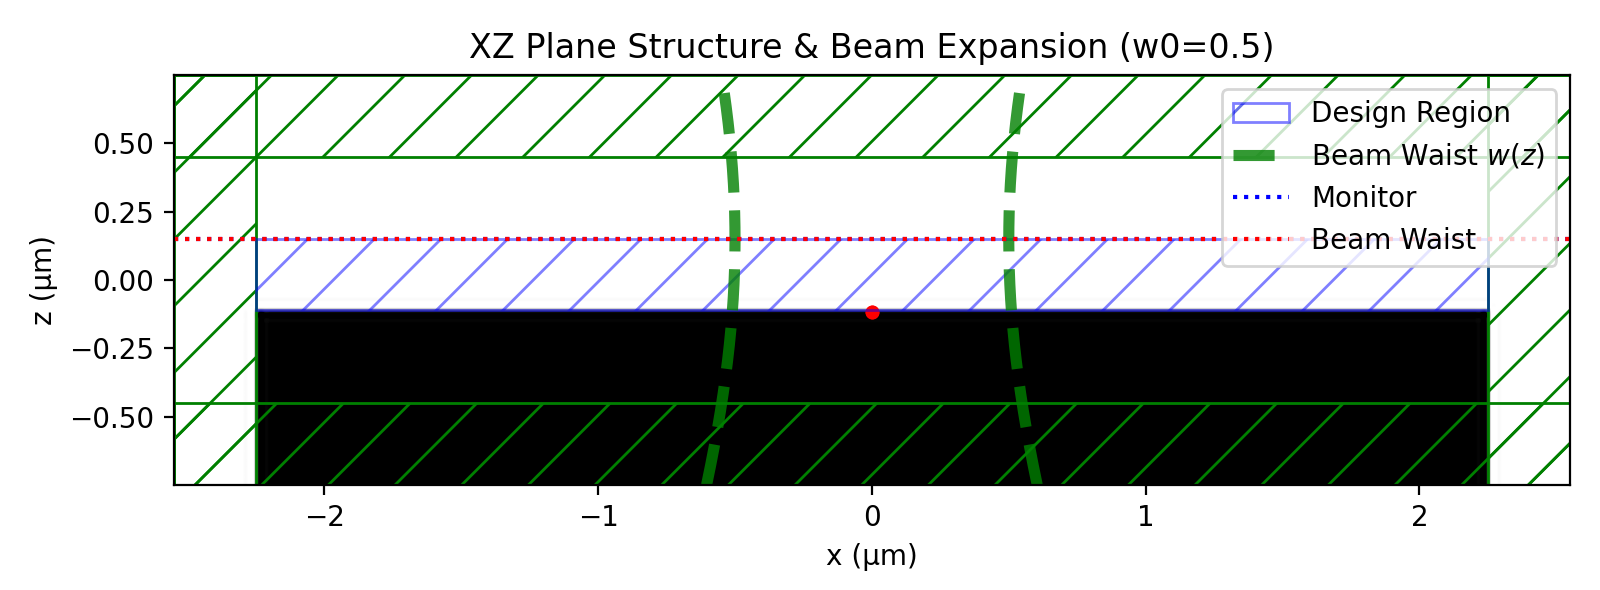
\includegraphics[width=1.0\textwidth]{img/xz_structure_waist.png}
\caption{Cross-sectional diagram of the simulation computational domain. From bottom to top: PML absorbing boundary (bottom), diamond substrate ($n=2.40$), monolayer WS$_2$ excitation layer (with circularly polarized dipole point source), GaP/air topology optimization design layer ($t_{\rm design}=0.257\;\mu$m), near-field monitor plane (red dashed line), air region, and PML (top and sides). The electromagnetic field collected by the near-field monitor is propagated to the far-field observation plane via near-to-far-field transformation (N2F).}
\label{fig:sim_geometry_a}
\end{figure}

\begin{figure}[htb]
\centering
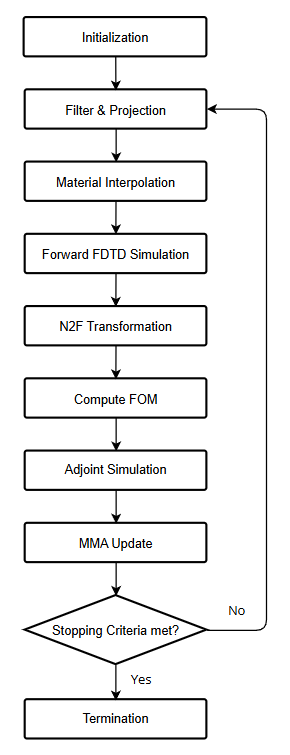
\includegraphics[width=1.0\textwidth,height=18cm,keepaspectratio]{img/workflow.png}
\caption{Topology optimization iteration flowchart. Each iteration performs, in order: forward FDTD simulation, N2F far-field transformation, FOM calculation, adjoint simulation, chain-rule gradient computation, and MMA update. After reaching the iteration limit, if $\beta < \beta_{\rm max}$, $\beta$ is increased and optimization continues (progressive binarization); once $\beta = \beta_{\rm max} = 512$ and convergence is reached, the final binarized structure $\bar{\rho}^*$ is output.}
\label{fig:opt_flowchart}
\end{figure} \newpage
\chapter{Results}

\label{ch:Results}

This chapter presents the results of six topology-optimized designs in a thematic comparative framework, covering target modes LG$_{\ell,0}$ for $\ell = 0$ through $\ell = 5$. Each section systematically compares all six datasets for the same physical quantity, highlighting how the topological charge affects design characteristics. Sections 4.5.3 and 4.7 are based on post-processing forward simulations re-run with the best density distribution $\bar{\rho}^{*}$ after optimization is complete ($\beta = 512$, final binarized structure); all other results display the best outcome found during optimization at the final $\beta = 512$ stage.

%===================================================================


\section{Optimization Process}

\label{sec:opt_process}

This section shows the convergence history of the six designs, including the $\beta$ schedule, FOM curves, and mode purity evolution, to verify the numerical stability of the $\beta$ continuation strategy.

\subsection{Beta Continuation Schedule and FOM Convergence}

\label{ssec:opt_FOM}

All six designs use the same $\beta$ schedule: starting from $\beta = 4$ and increasing at fixed iteration intervals to a final $\beta = 512$, with each $\beta$ switch marked by a purple vertical line (see Figure~\ref{fig:FOM_history_all}). The FOM curves for all designs show a large upward trend during the $\beta < 16$ stage, reaching their highest values near the end of this interval. This convergence pattern reflects the fact that the looser boundary conditions at low $\beta$ allow the optimizer to explore the continuous density space freely and efficiently find globally better topological layouts that achieve peak performance.

The final FOM values for low topological charges $\ell = 0, 1$ ($0.39$ and higher) are noticeably higher than for high topological charges $\ell = 3, 4, 5$ (FOM $\approx 0.30$ to $0.19$), indicating that higher-order OAM modes require more complex phase modulation, which limits the final coupling efficiency. Notably, although the FOM value for $\ell = 3$ is slightly lower, performance recovers very quickly after each $\beta$ switch, showing that increasing the topological charge does not significantly worsen the convergence behavior.

\begin{figure}[htb]
\centering
	\begin{tabular}{cc} 
	    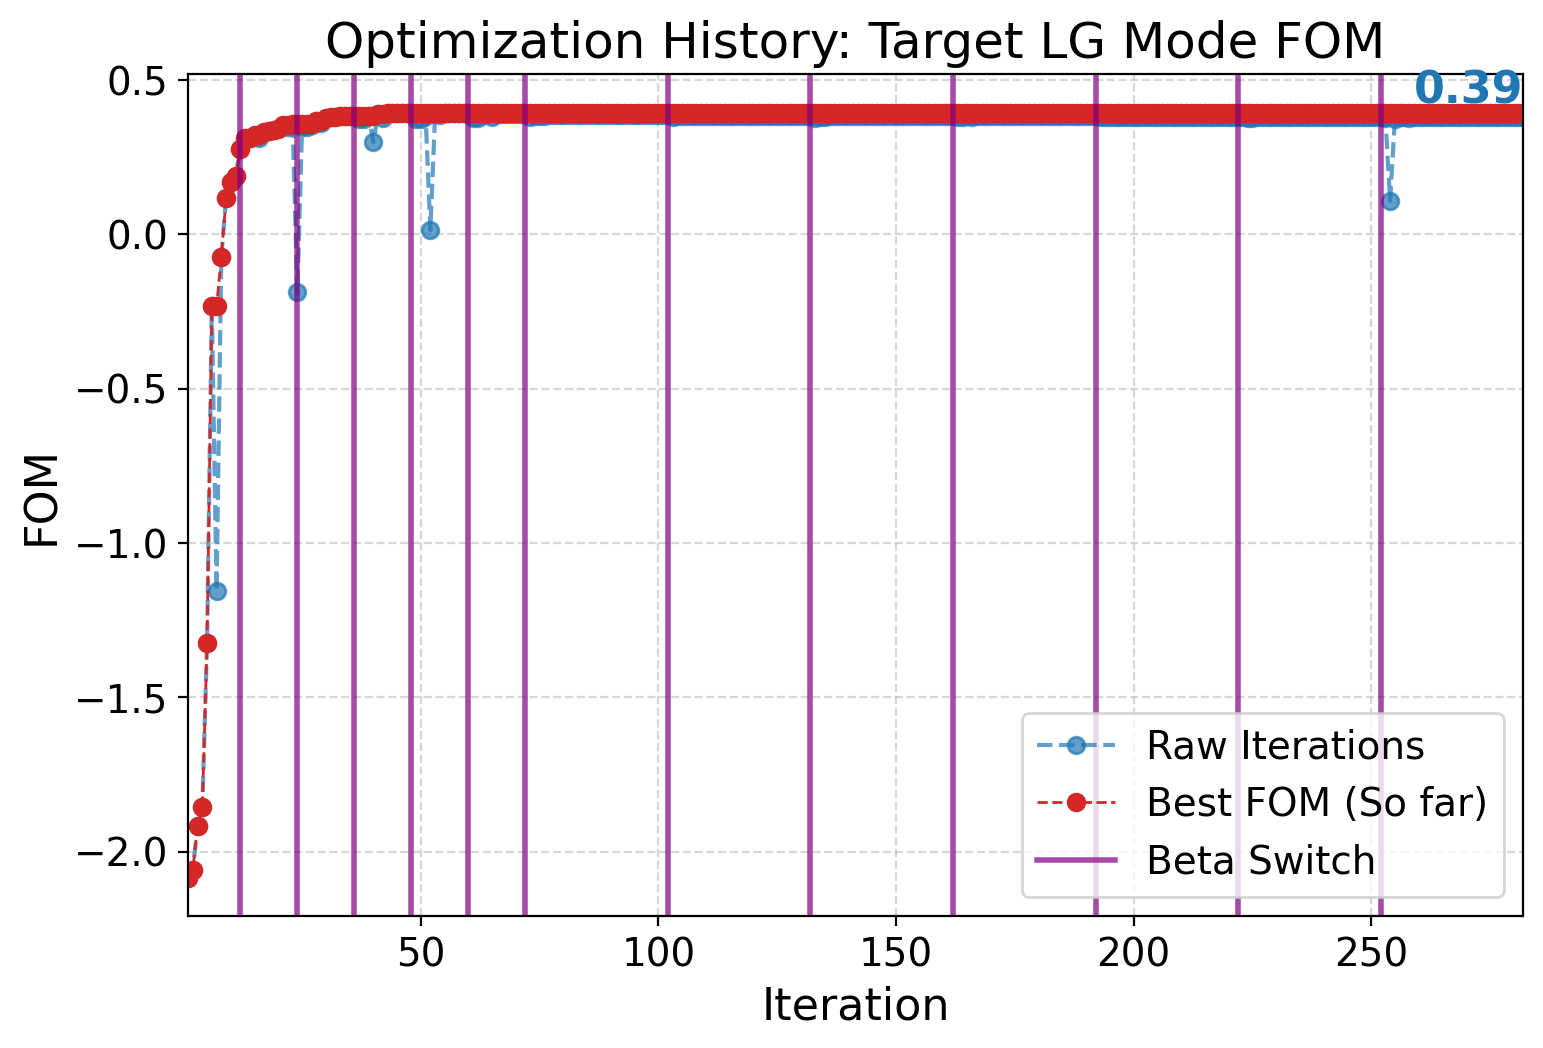
\includegraphics[width=0.47\textwidth]{img/017_FOM_history_staircase.png} &
	    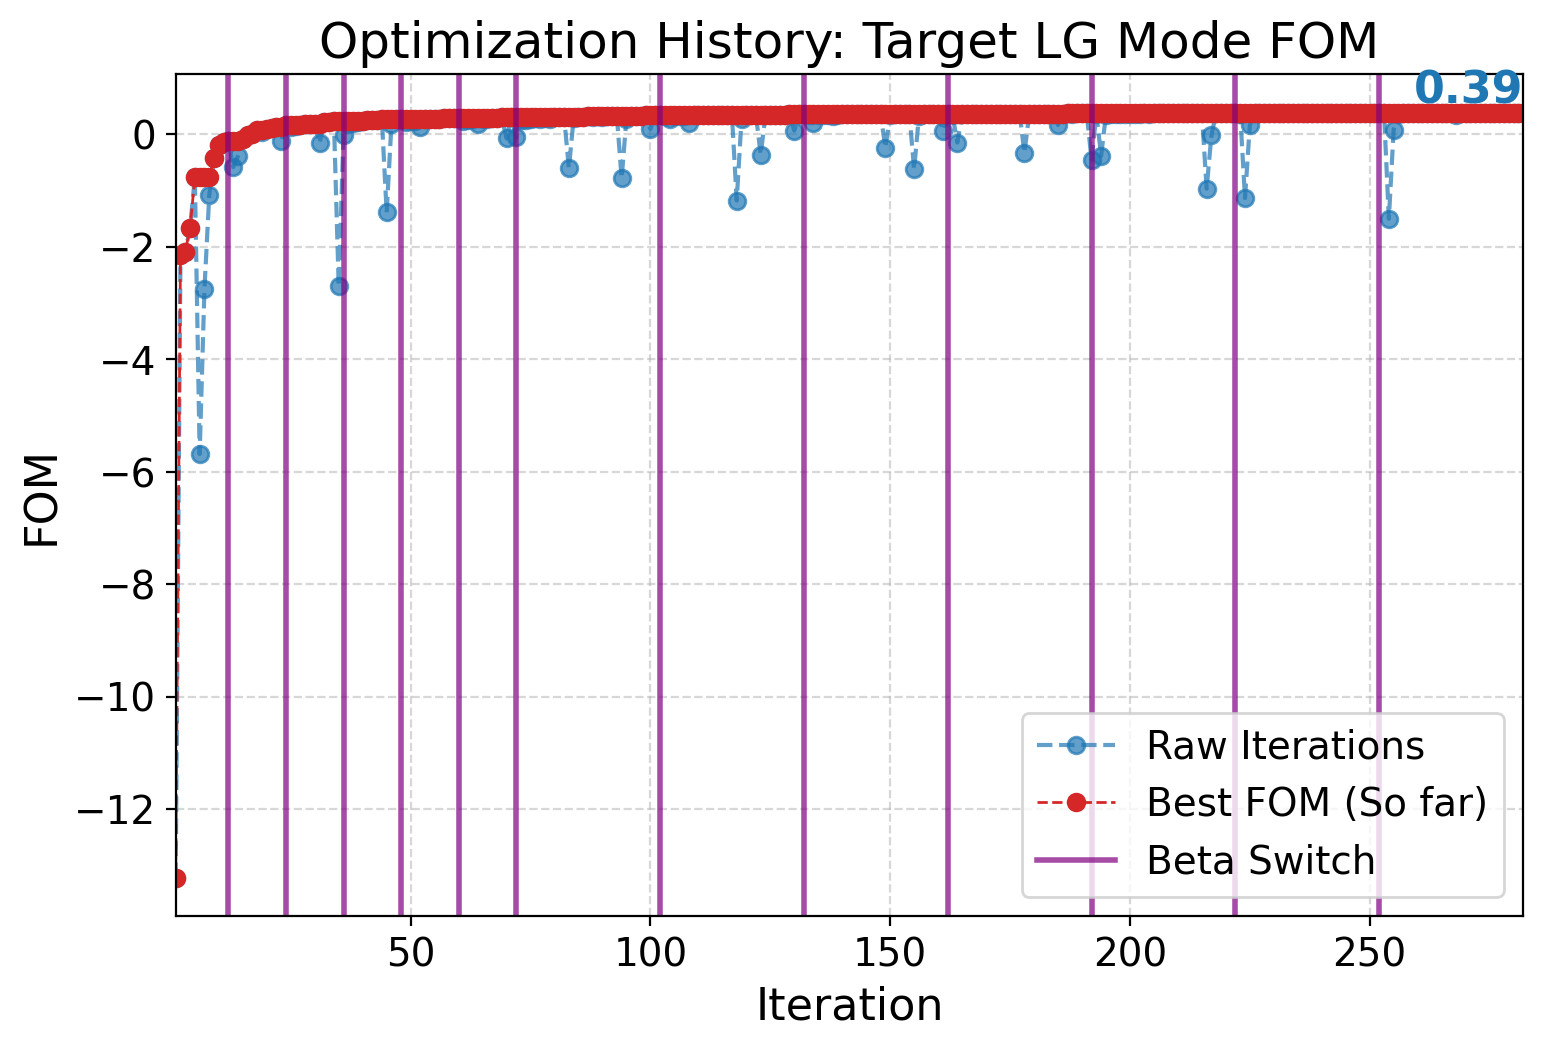
\includegraphics[width=0.47\textwidth]{img/018_FOM_history_staircase.png}
		\\ (a) & (b) \\[6pt]
		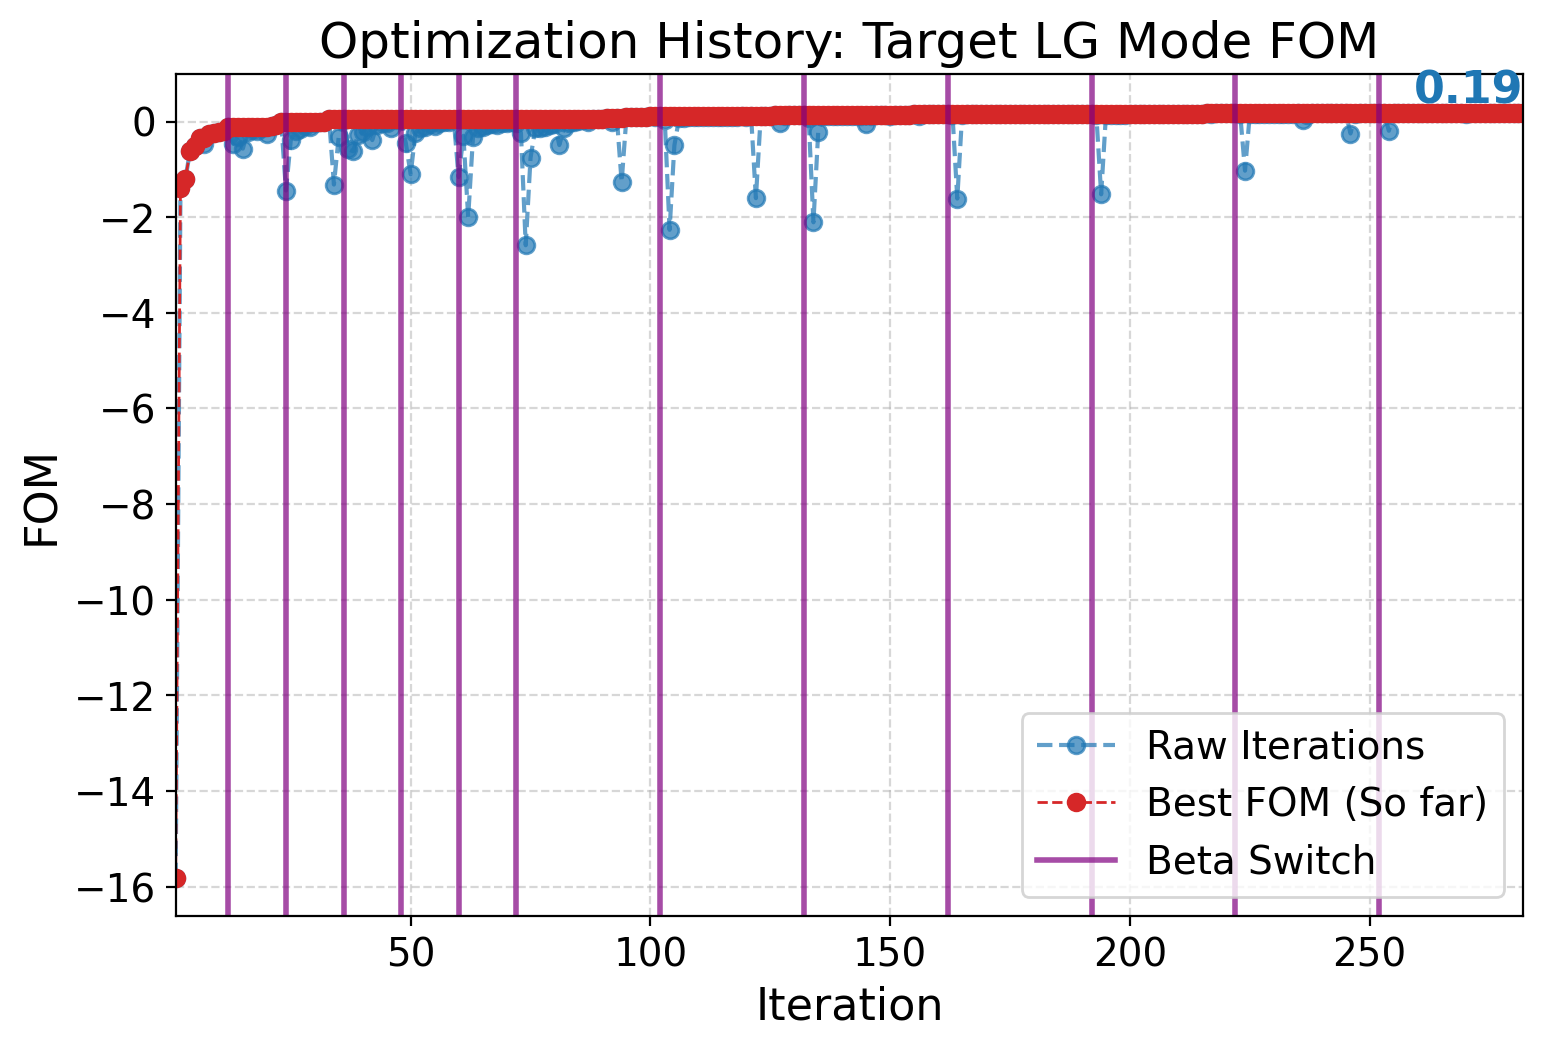
\includegraphics[width=0.47\textwidth]{img/013_FOM_history_staircase.png}&
		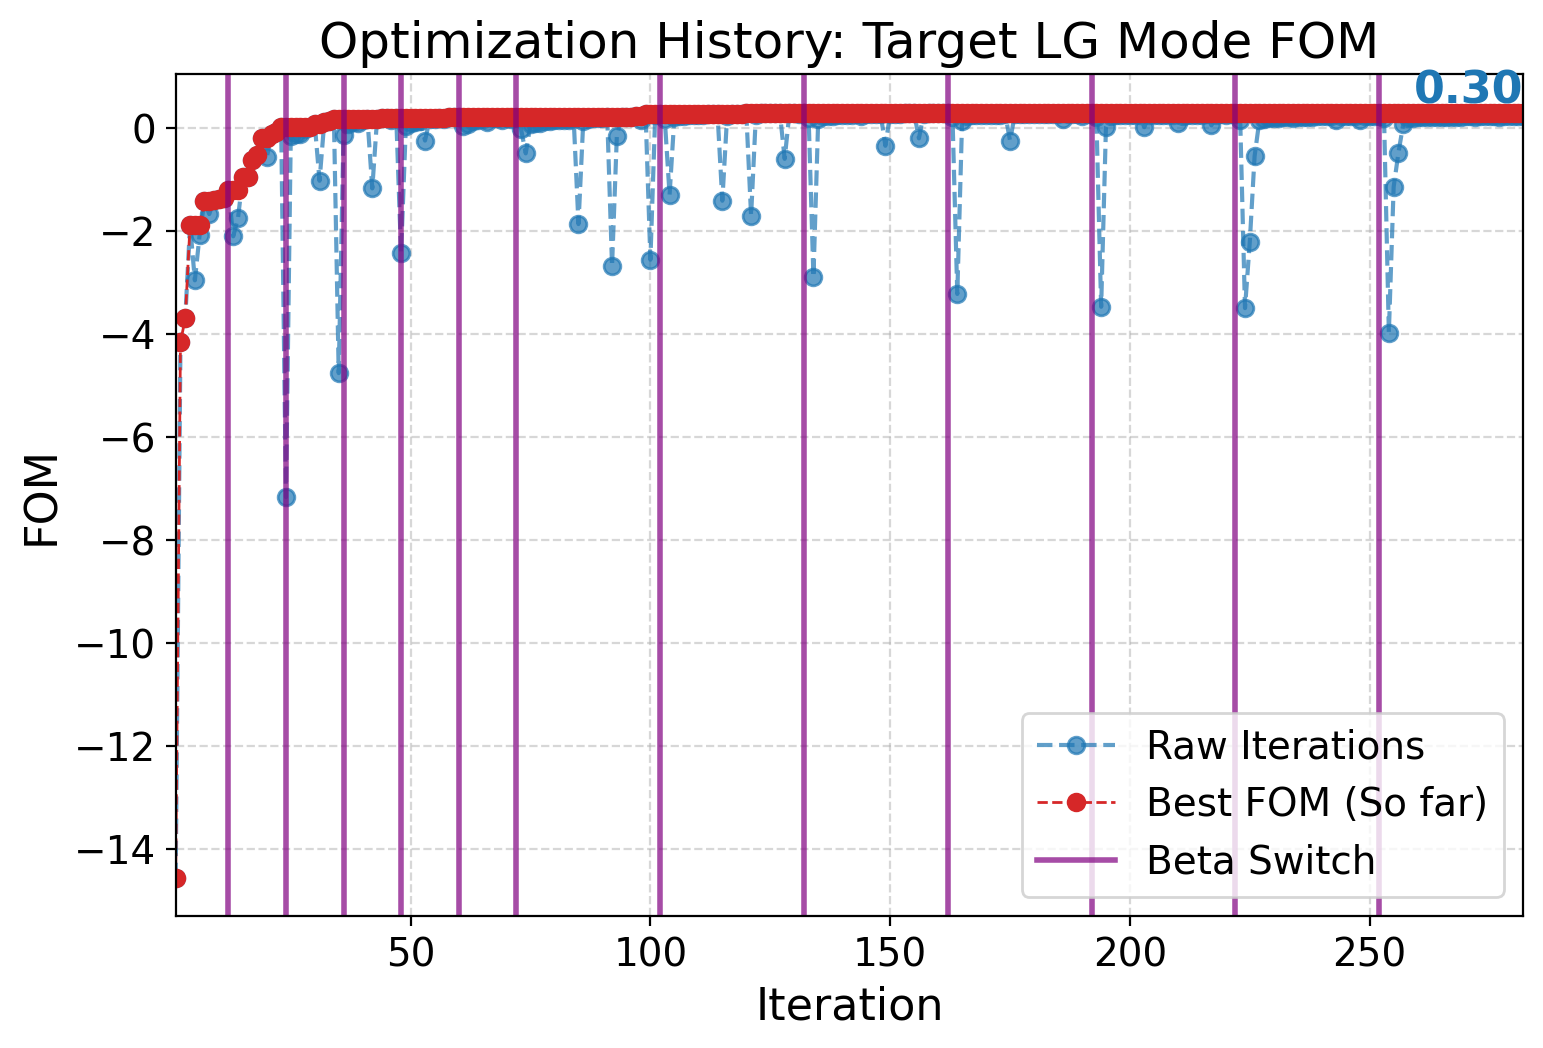
\includegraphics[width=0.47\textwidth]{img/020_FOM_history_staircase.png}
	    \\  (c)  & (d) \\[6pt]
	    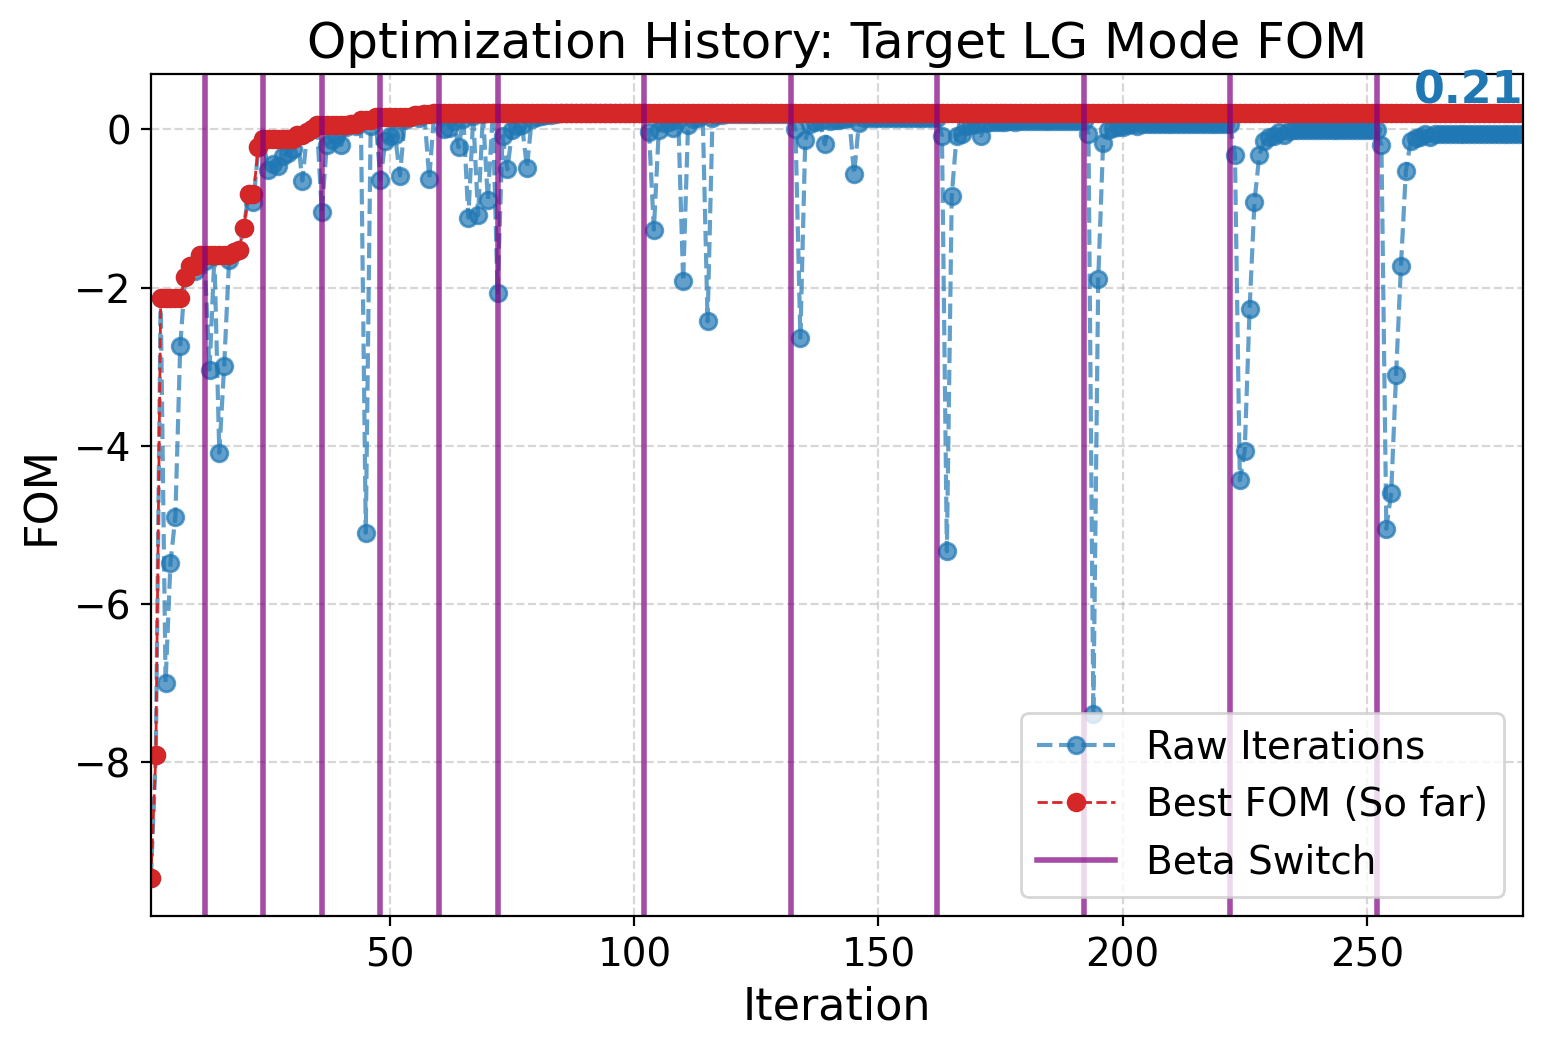
\includegraphics[width=0.47\textwidth]{img/021_FOM_history_staircase.png}&
	    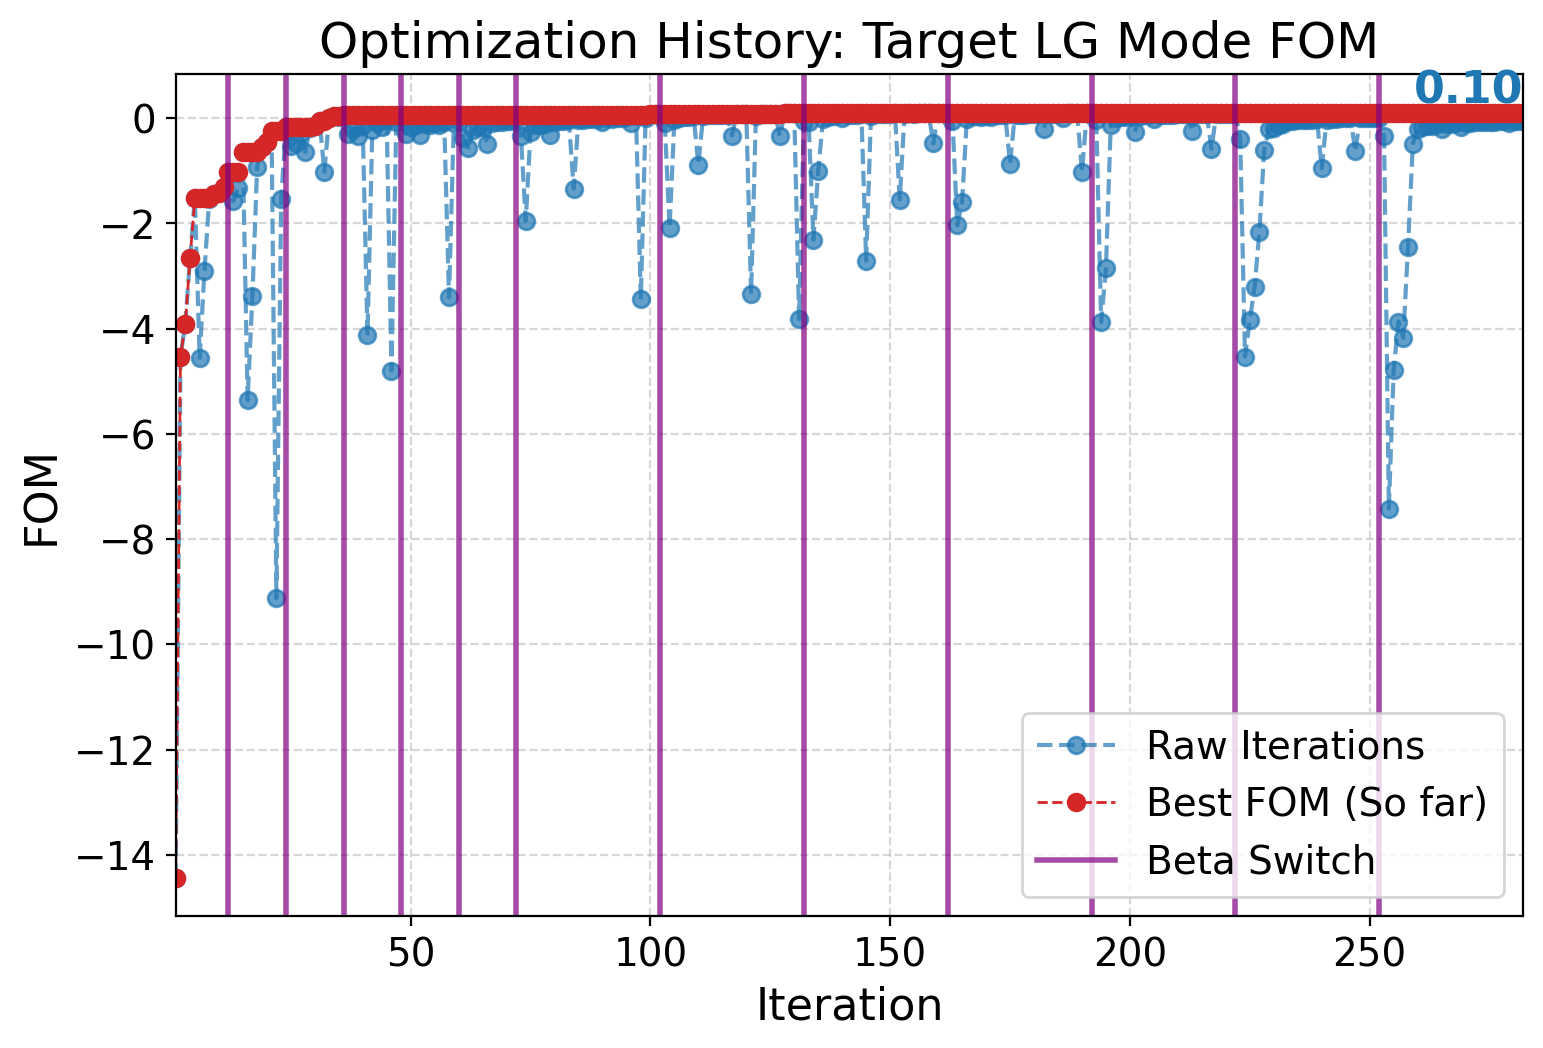
\includegraphics[width=0.47\textwidth]{img/022_FOM_history_staircase.png}
	    \\ (e) & (f)
	\end{tabular}
\caption{FOM convergence history: (a)$\sim$(f) $\ell \in \{0, 1, 2, 3, 4, 5\}$, respectively. Blue dashed line: raw FOM value at each iteration; red dashed line: best-so-far tracking value; purple vertical lines: $\beta$ continuation switch points ($\beta_\text{final} = 512$).}
\label{fig:FOM_history_all}
\end{figure}




\subsection{Mode Purity Convergence}

\label{ssec:opt_purity}

Figure~\ref{fig:purity_history_all} shows the mode purity convergence history for the six designs. The purity evolution closely tracks the FOM history: the main structure forms rapidly in the early stage, and purity saturates and stabilizes after the 2nd to 4th $\beta$ switches.

Low topological charge designs $\ell = 0, 1, 2$ all achieve final purity above $96\%$, with $\ell = 1$ reaching the highest of all six at $98.66\%$, indicating the best solution quality under these design conditions. As topological charge increases, $\ell = 3$ drops to $94.13\%$, while $\ell = 4$ and $\ell = 5$ fall further to $81.94\%$ and $82.62\%$. In the high topological charge cases, the finite $4.5\;\mu\text{m}$ design area size and resolution limit mean the high-order OAM modes are approaching their physical limits. Purity therefore hits a ceiling early in the optimization, and further increases in $\beta$ only cause structural boundary oscillations without improving the final purity.

The final quantitative results for $\ell = 0$ to $5$ are summarized in Table~\ref{tab:results_summary}.

\begin{figure}[htb]
\centering
	\begin{tabular}{cc} 
	    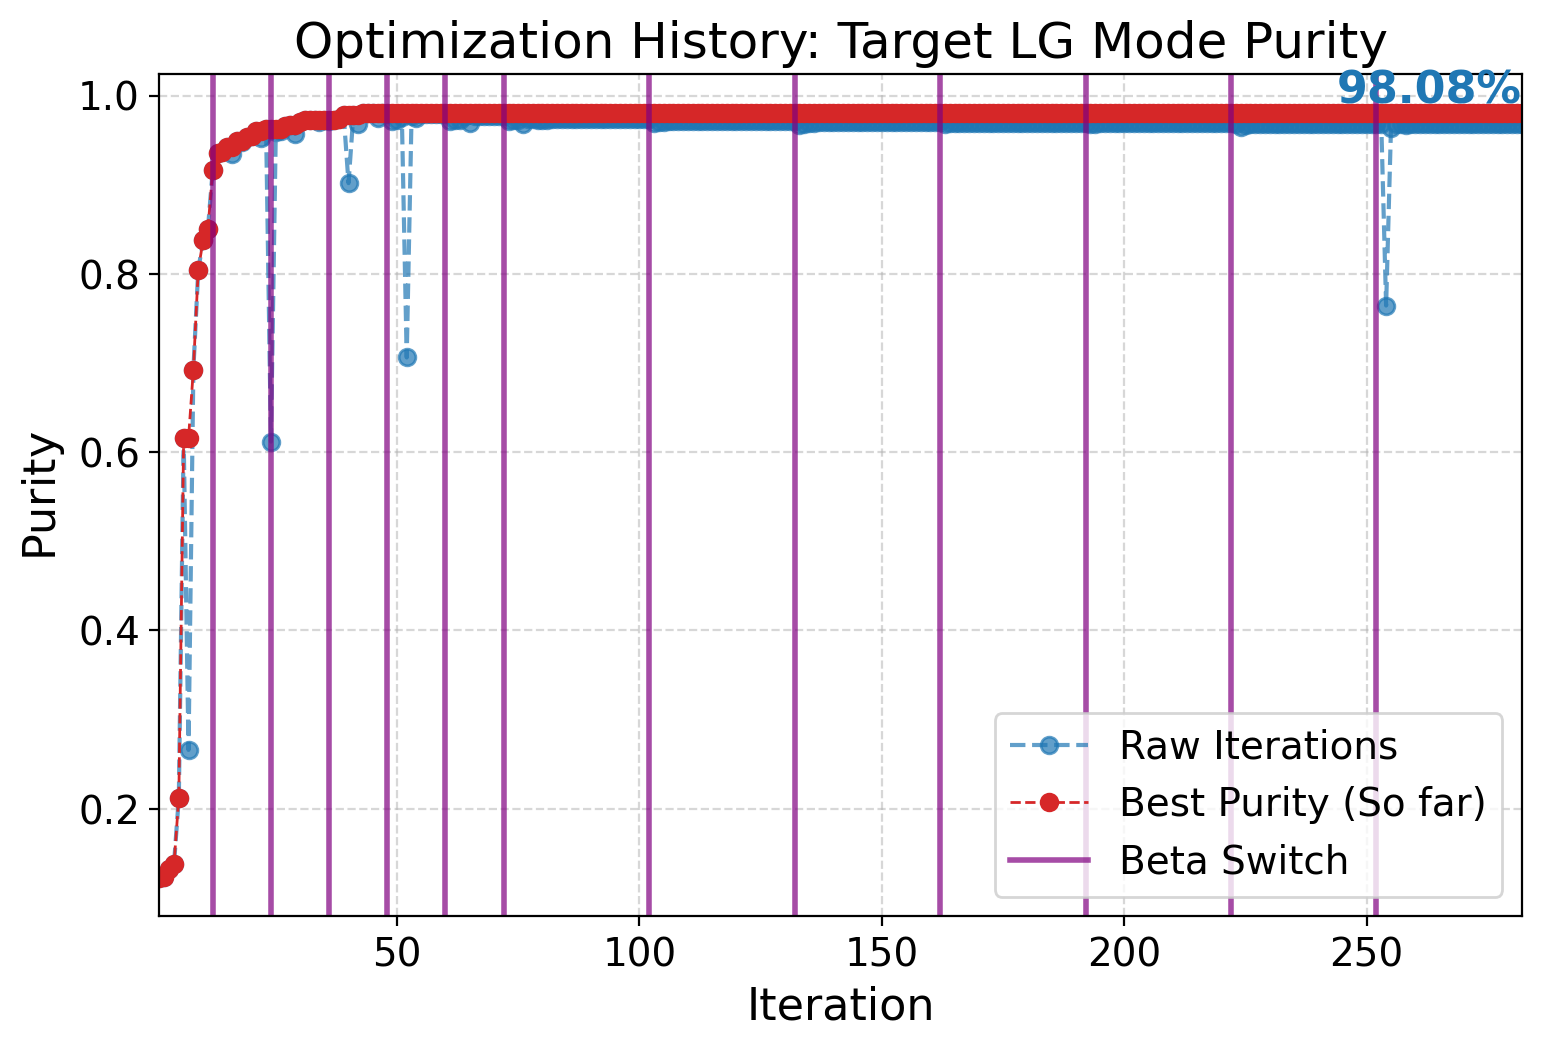
\includegraphics[width=0.47\textwidth]{img/017_purity_history_staircase.png}&
	    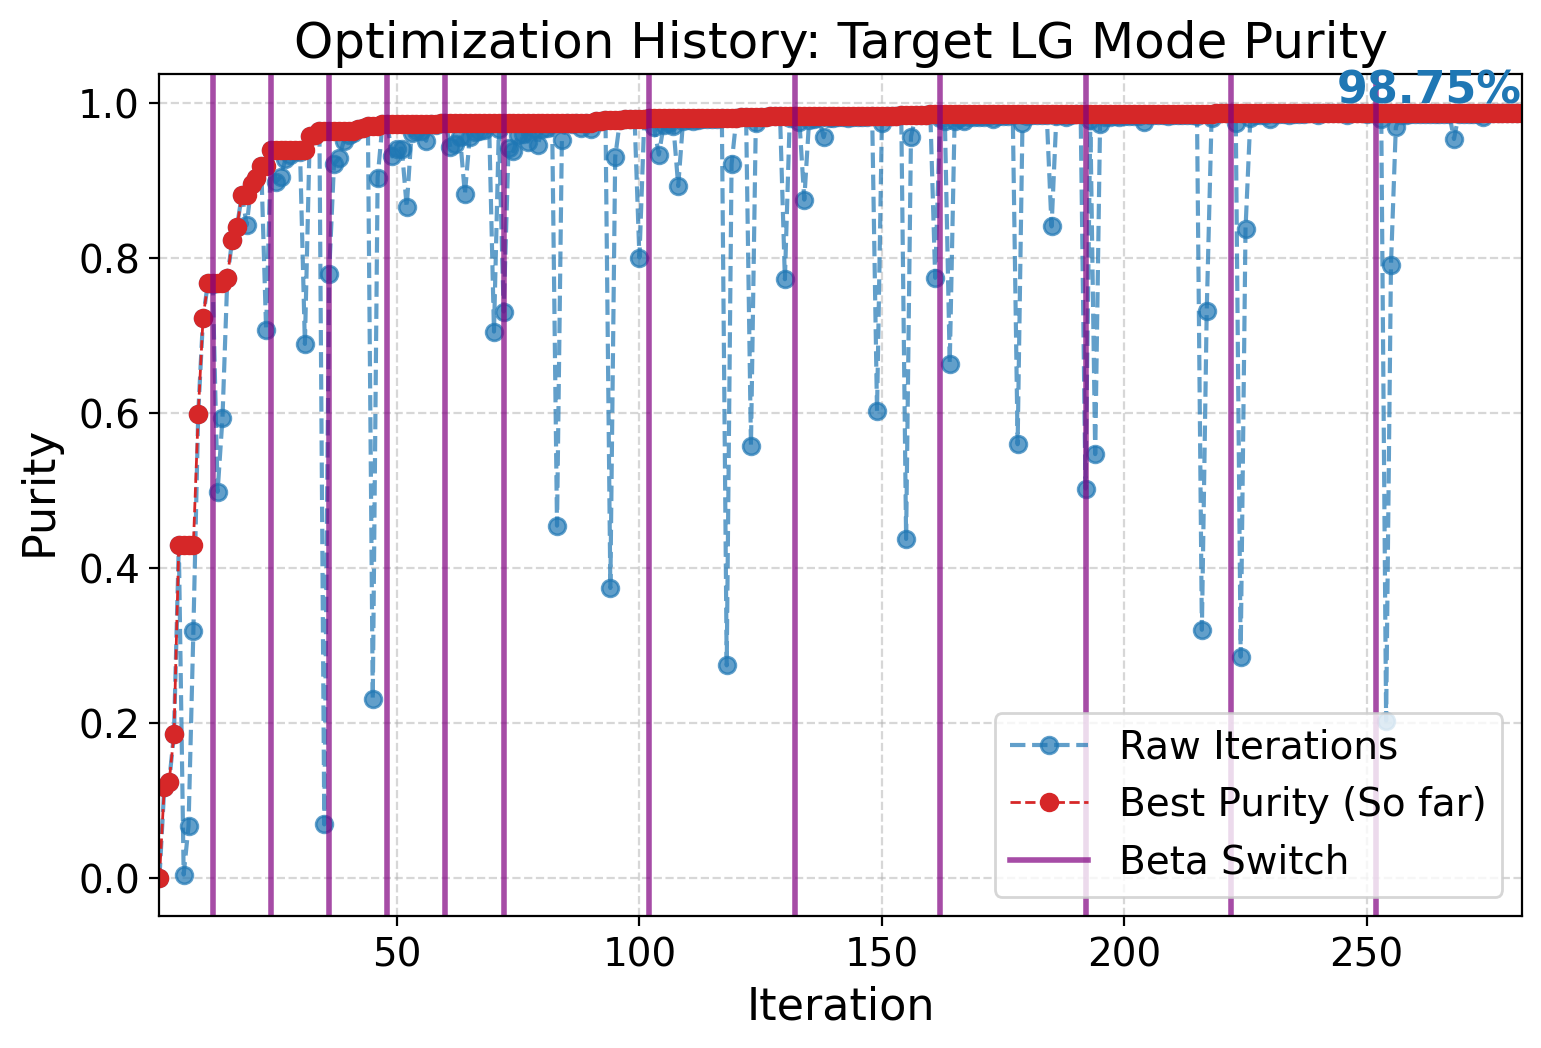
\includegraphics[width=0.47\textwidth]{img/018_purity_history_staircase.png}
		\\ (a) & (b) \\[6pt]
		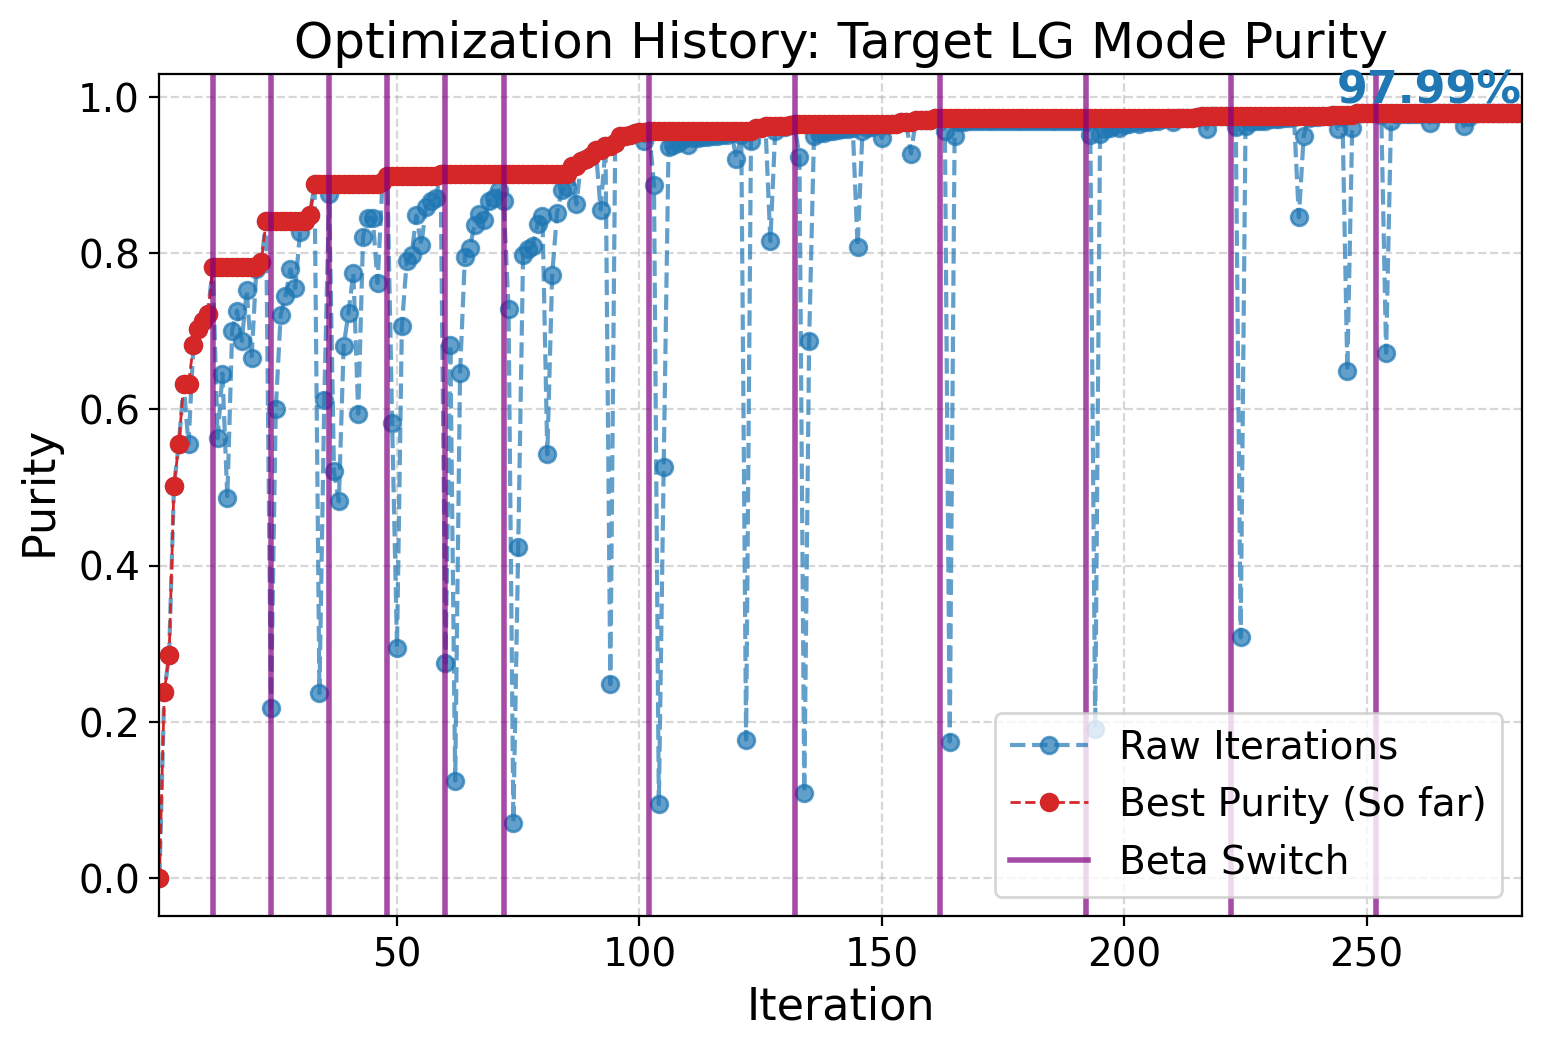
\includegraphics[width=0.47\textwidth]{img/013_purity_history_staircase.png}&
	    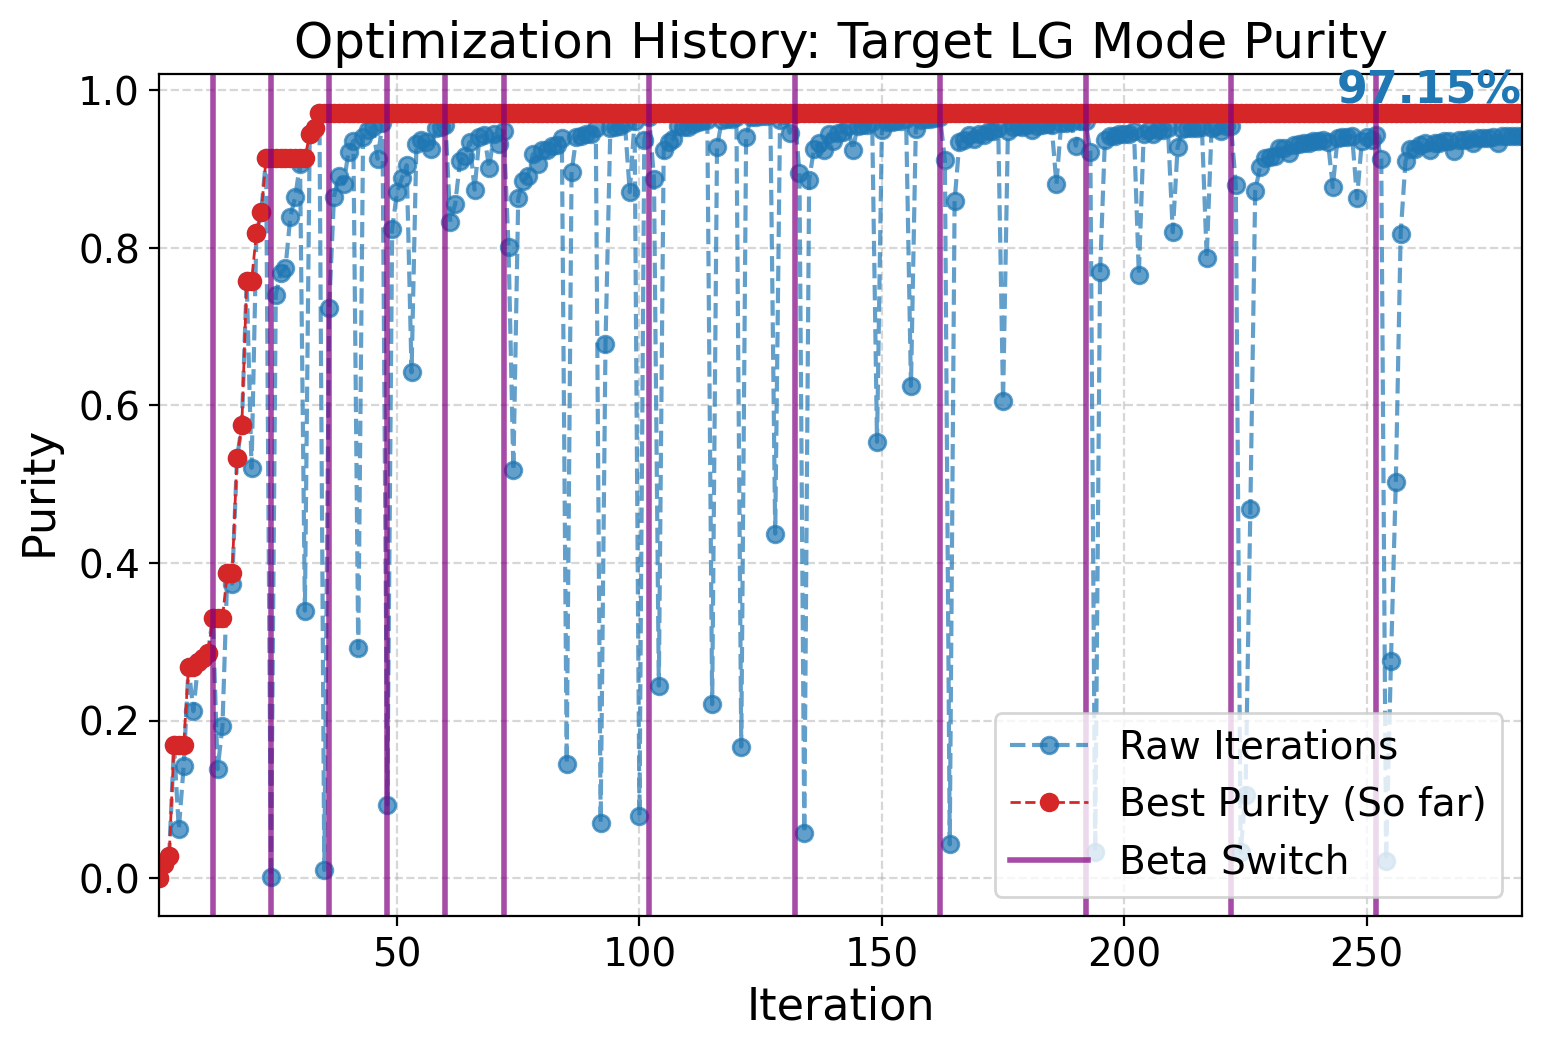
\includegraphics[width=0.47\textwidth]{img/020_purity_history_staircase.png}
	    \\  (c) & (d)\\[6pt]
	    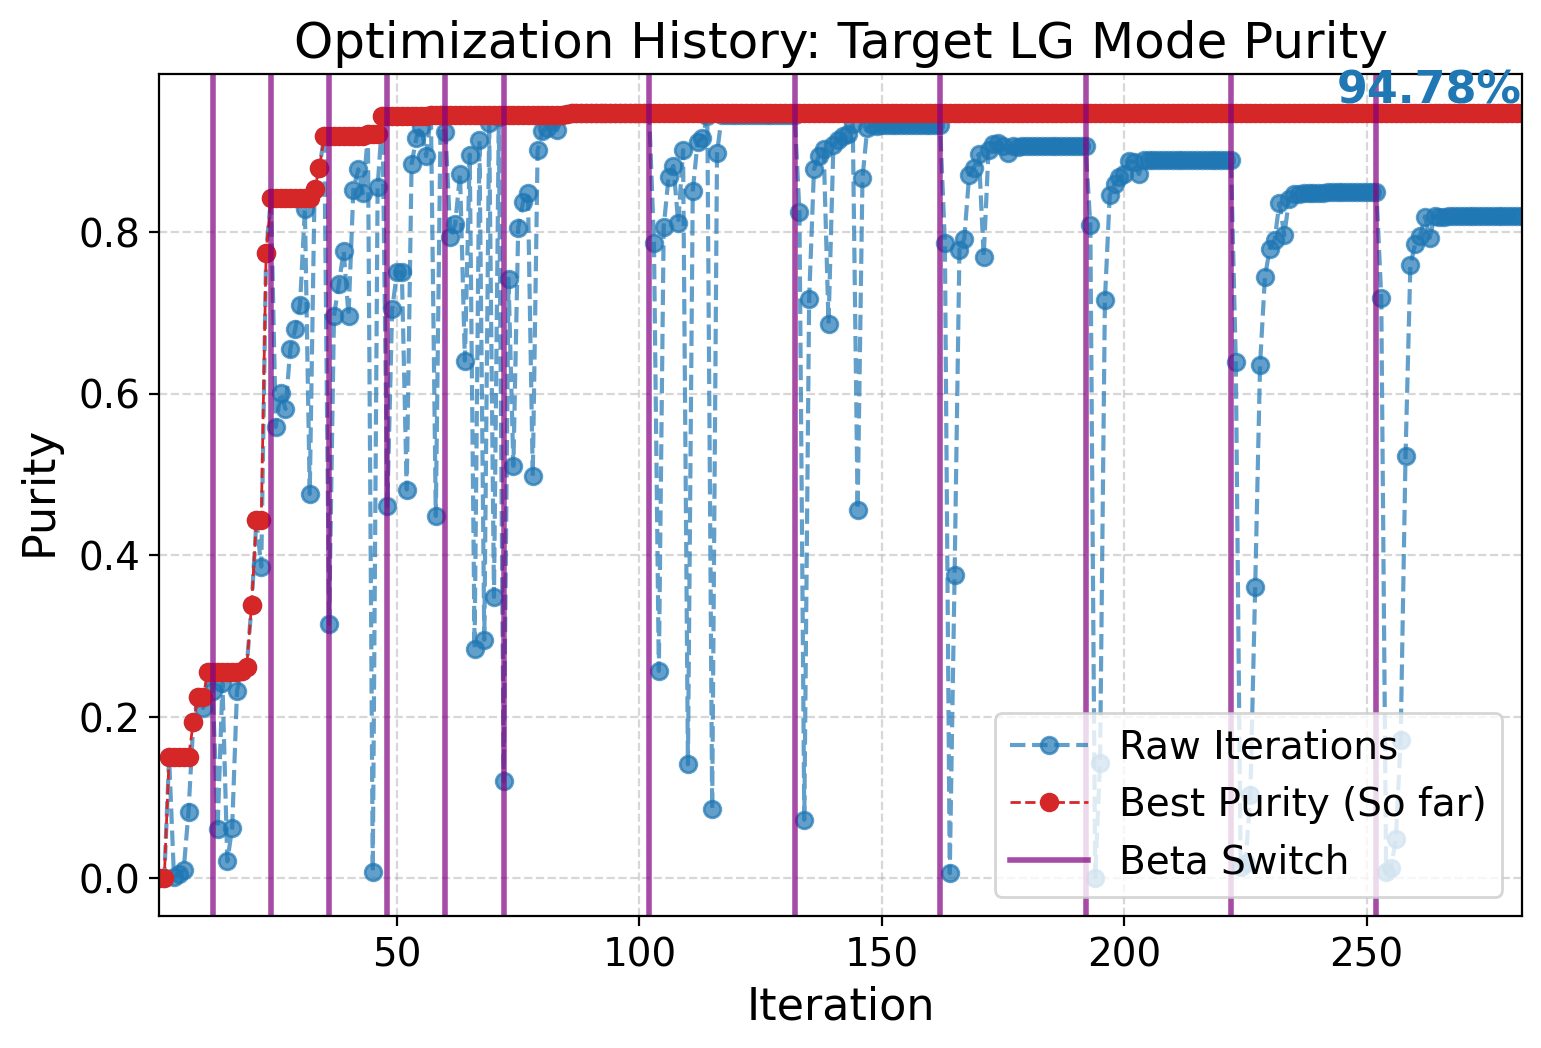
\includegraphics[width=0.47\textwidth]{img/021_purity_history_staircase.png}&
	    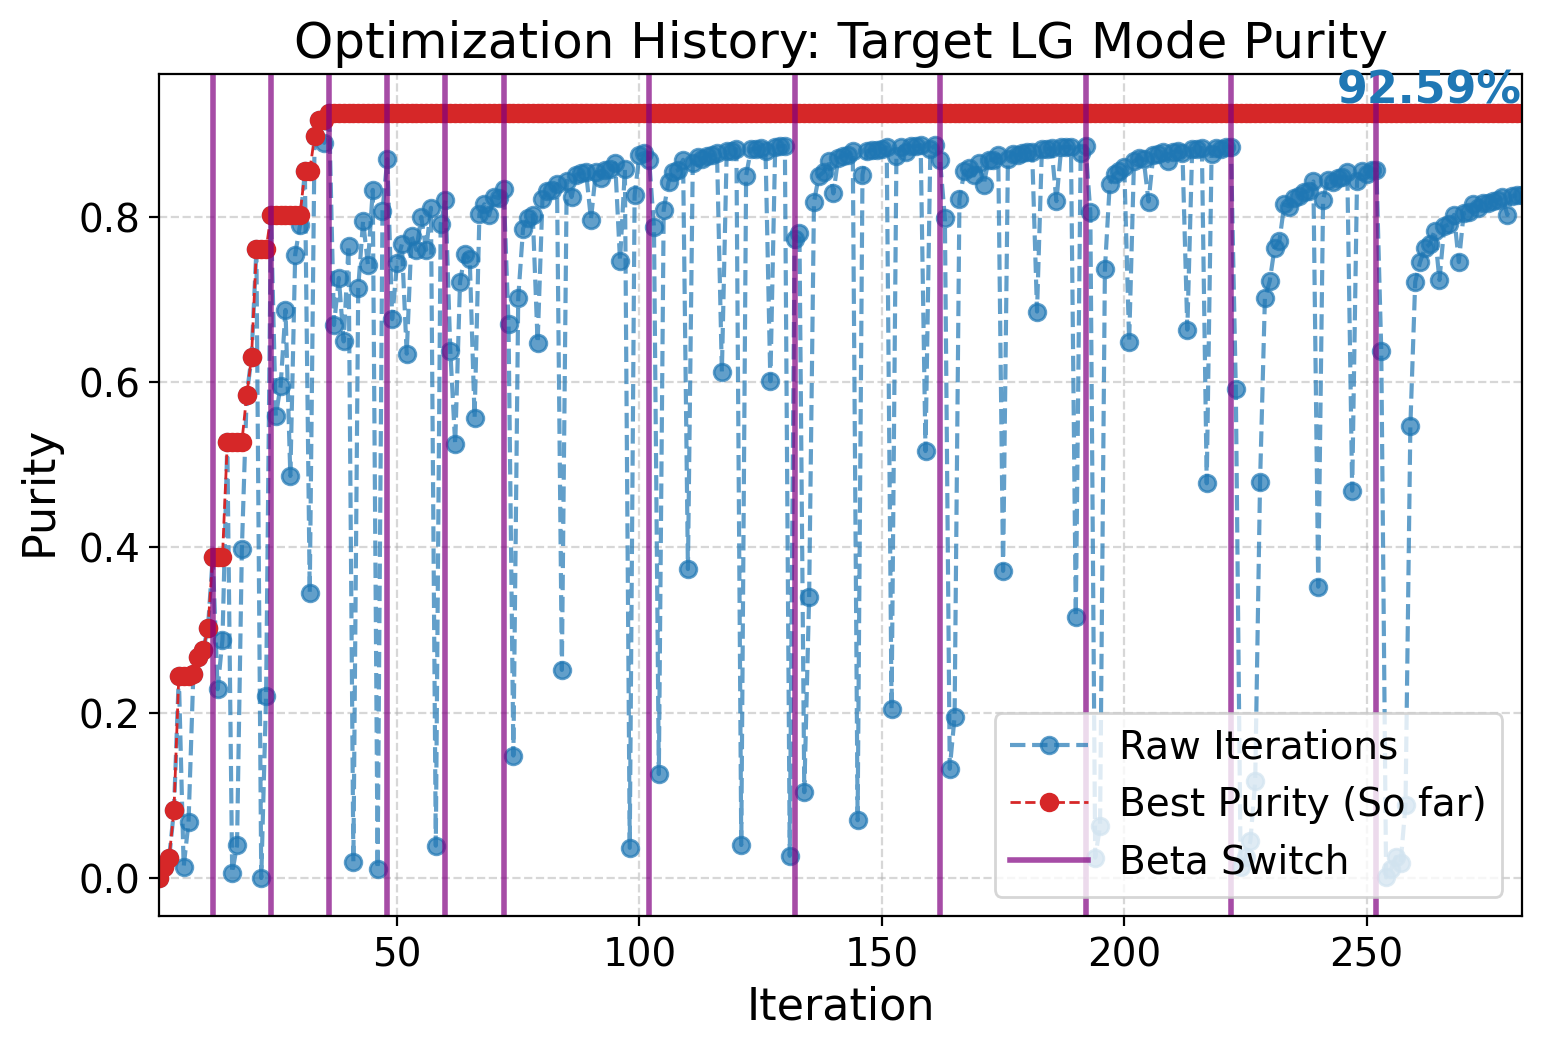
\includegraphics[width=0.47\textwidth]{img/022_purity_history_staircase.png}
	    \\ (e) & (f) 
	\end{tabular}
\caption{Mode purity convergence history: (a)$\sim$(f) $\ell \in \{0, 1, 2, 3, 4, 5\}$, respectively. Blue dashed line: instantaneous value at each iteration; red dashed line: best-so-far tracking value; purple vertical lines: $\beta$ switch points. The final best purity value is indicated in the upper right corner.}
\label{fig:purity_history_all}
\end{figure}



\begin{table}[htb]
\centering
\caption{Performance summary for $\ell = 0$ to $5$ (far-field plane at $z = 10\,z_R$).}
\label{tab:results_summary}
    \begin{tabular}{ccccc}
        \hline
        $\ell$ & Target mode & Purity (\%) & $|\text{Overlap}|^{2}$ & FOM\\
        \hline
        0 & LG$_{0,0}$ & 96.81 & 60.92 & 0.38\\
        1 & LG$_{1,0}$ & 98.66 & 53.88 &  0.39\\
        2 & LG$_{2,0}$ & 97.96 & 7.99 & 0.19\\
        3 & LG$_{3,0}$ & 94.13 & 18.69 & 0.23\\
        4 & LG$_{4,0}$ & 81.94 & 4.00 & -0.06 \\
        5 & LG$_{5,0}$ & 82.62 & 3.96 & -0.05\\
        \hline
    \end{tabular}
\end{table}

%===================================================================

\section{Optimized Structures}

\label{sec:structures}


Figure~\ref{fig:structures_all} shows the final converged GaP/air binary material density distributions for the six designs (black represents GaP, refractive index $n = 3.31$; white represents air, refractive index $n = 1$).

Examining the six structures, the most visually striking feature appears in the $\ell = 2$ design (Figure~\ref{fig:structures_all}(c)): a clear two-arm spiral pattern is visible at the center, closely resembling the working principle of a spiral phase plate (SPP). This suggests that the optimizer, guided by adjoint gradients, spontaneously discovers a design strategy similar to a two-arm SPP to provide the required $2 \times 2\pi$ azimuthal phase modulation. The surrounding scattering features act as a compensation mechanism to correct near-field coupling errors and improve far-field mode shaping accuracy.

For the other designs, the structures do not show simple $\ell$-fold rotational spiral features. $\ell = 0$ shows a roughly symmetric closed GaP core at the center; $\ell = 1, 3, 4, 5$ produce free-form, non-intuitive material distributions with no obvious geometric regularity. This reflects the nature of topology optimization: when the SPP-like spiral strategy is not the globally optimal solution, the optimizer automatically searches for an alternative distribution that better satisfies the gradient conditions, even if the result has no geometric symmetry that is easy to interpret visually.

The exclusive appearance of the $\ell$-fold spiral structure in the $\ell = 2$ design, and its absence in all other designs, can be understood through a discrete rotational symmetry selection rule discussed in Section~\ref{ssec:spiral_emergence}.

Despite the different geometric forms, all six structures show dense scattering features away from the center. As topological charge increases, these surrounding features become denser, reflecting the higher modulation demand on azimuthal phase space for higher-order OAM modes.


\begin{figure}[htb]
\centering
    \begin{tabular}{ccc}
        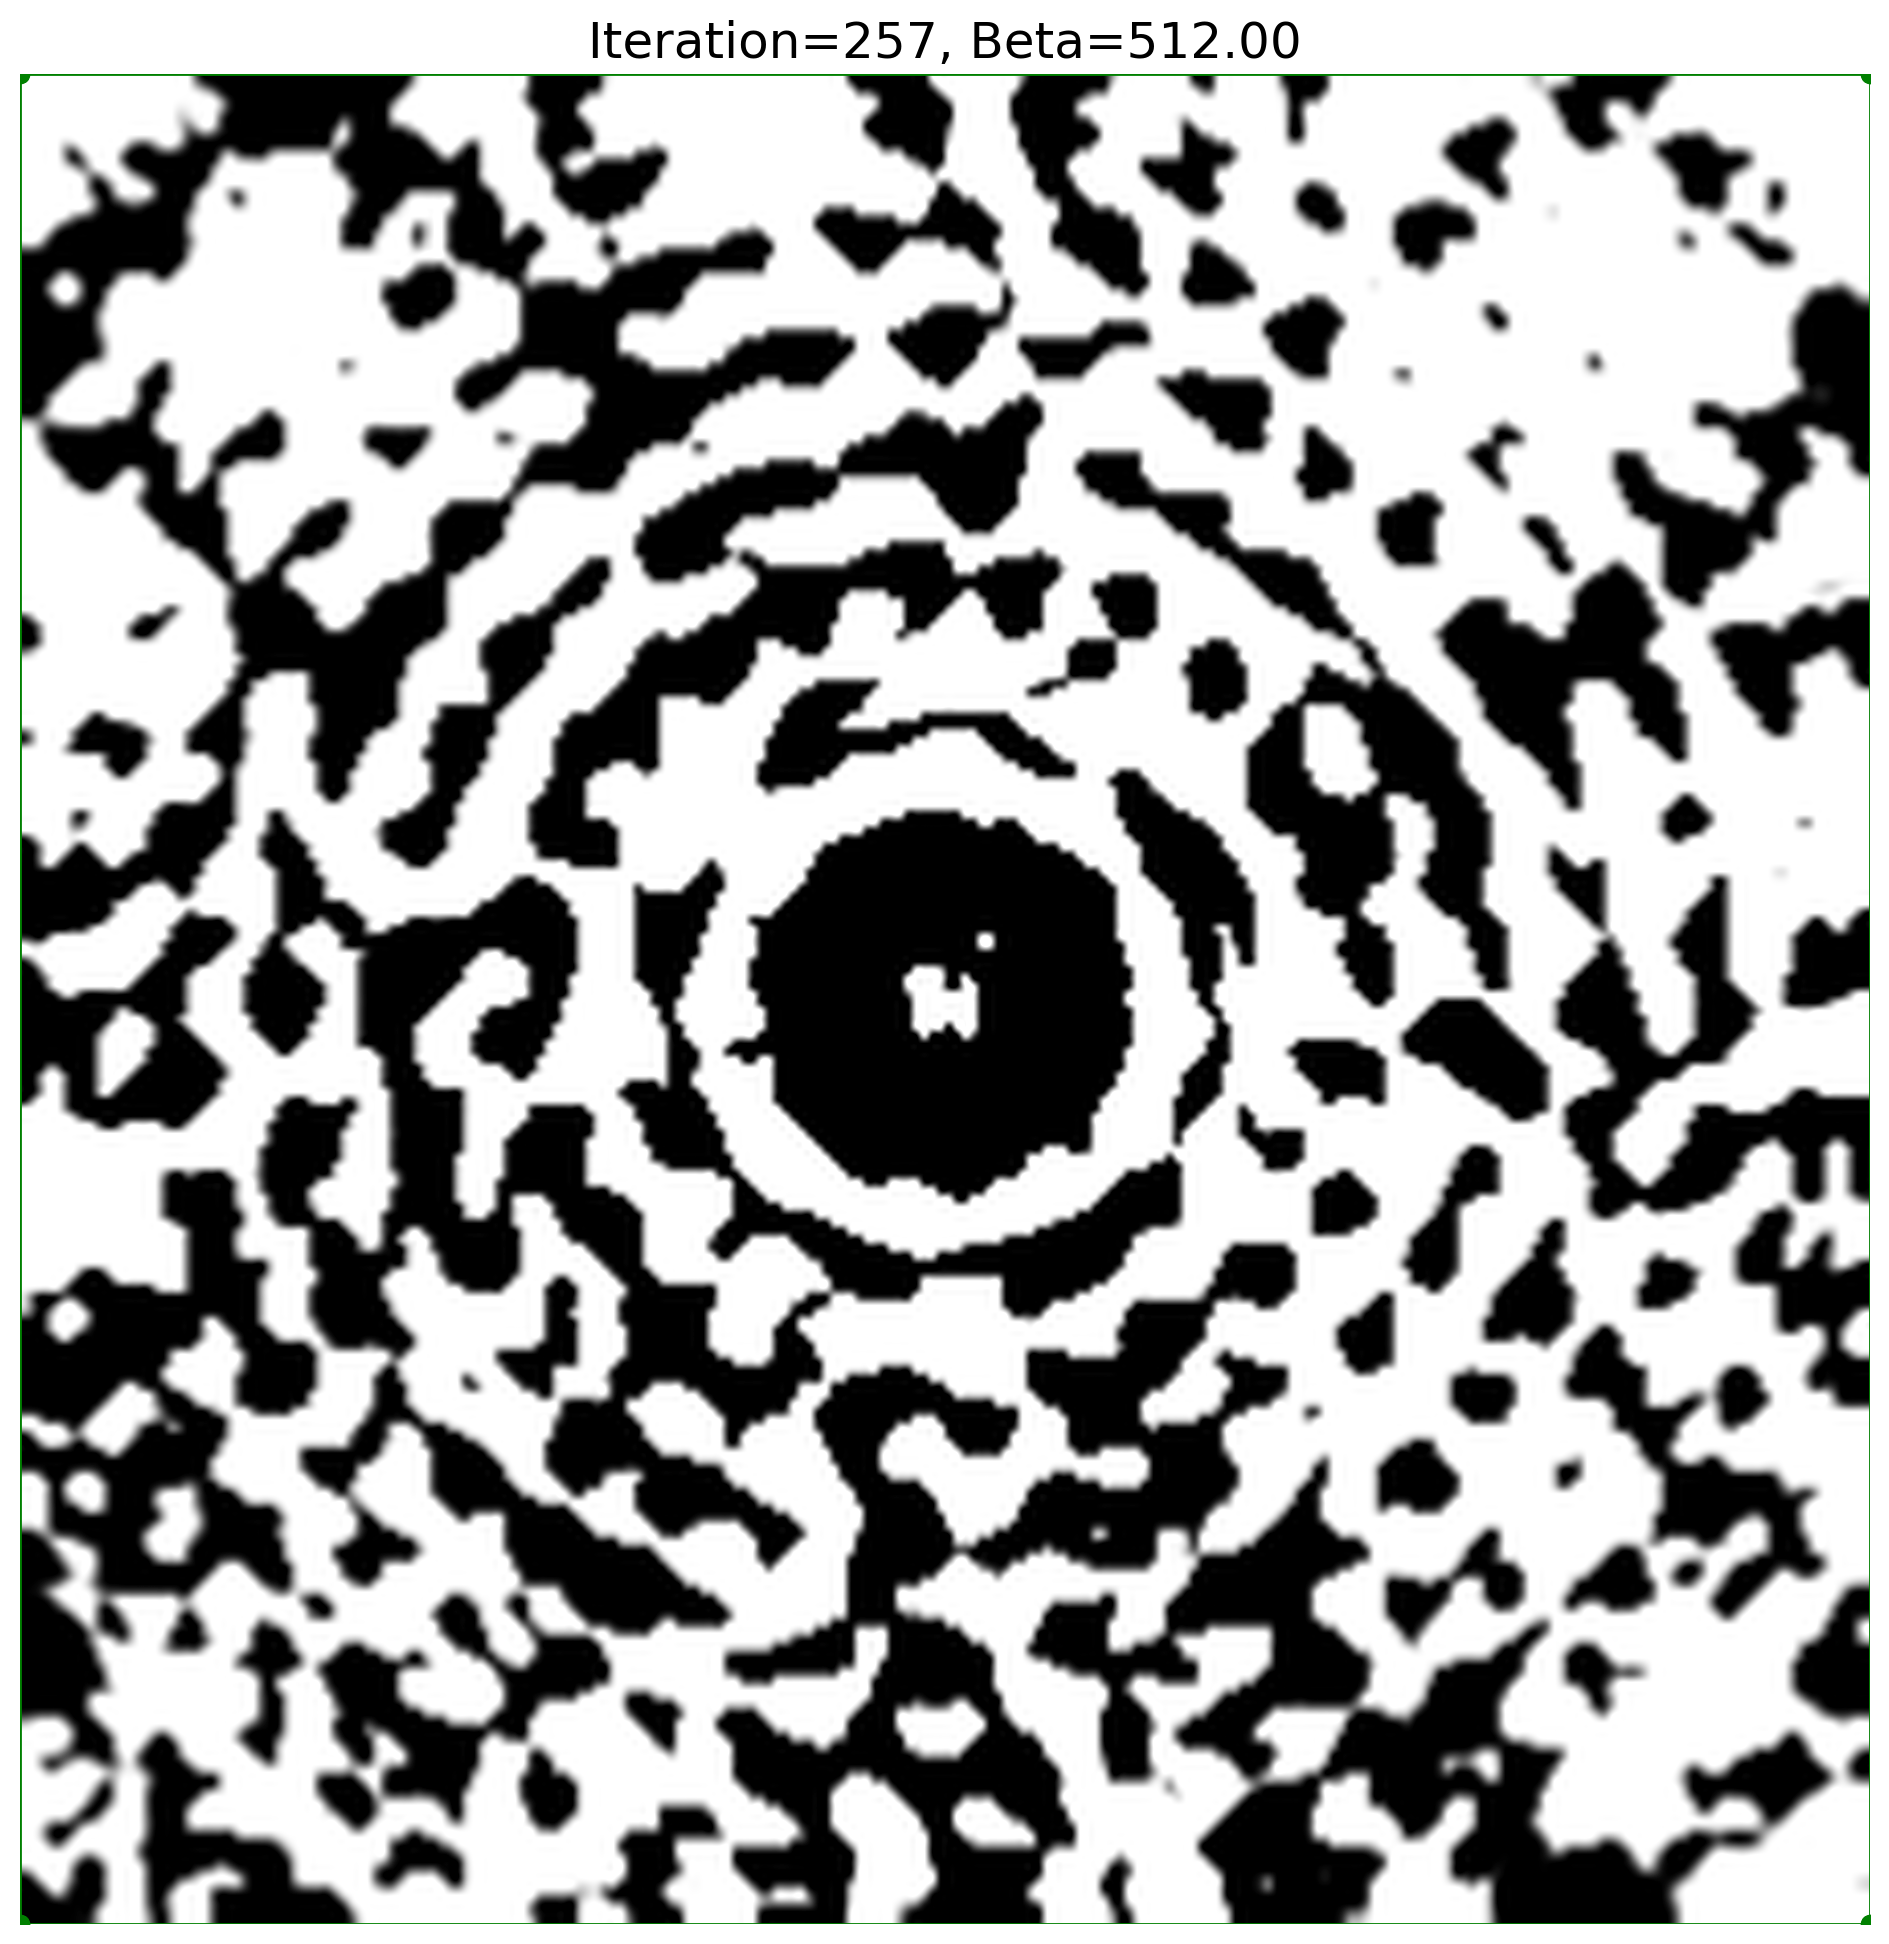
\includegraphics[width=0.3\textwidth]{img/017_structure_iter_257_beta_512.00.png} &
        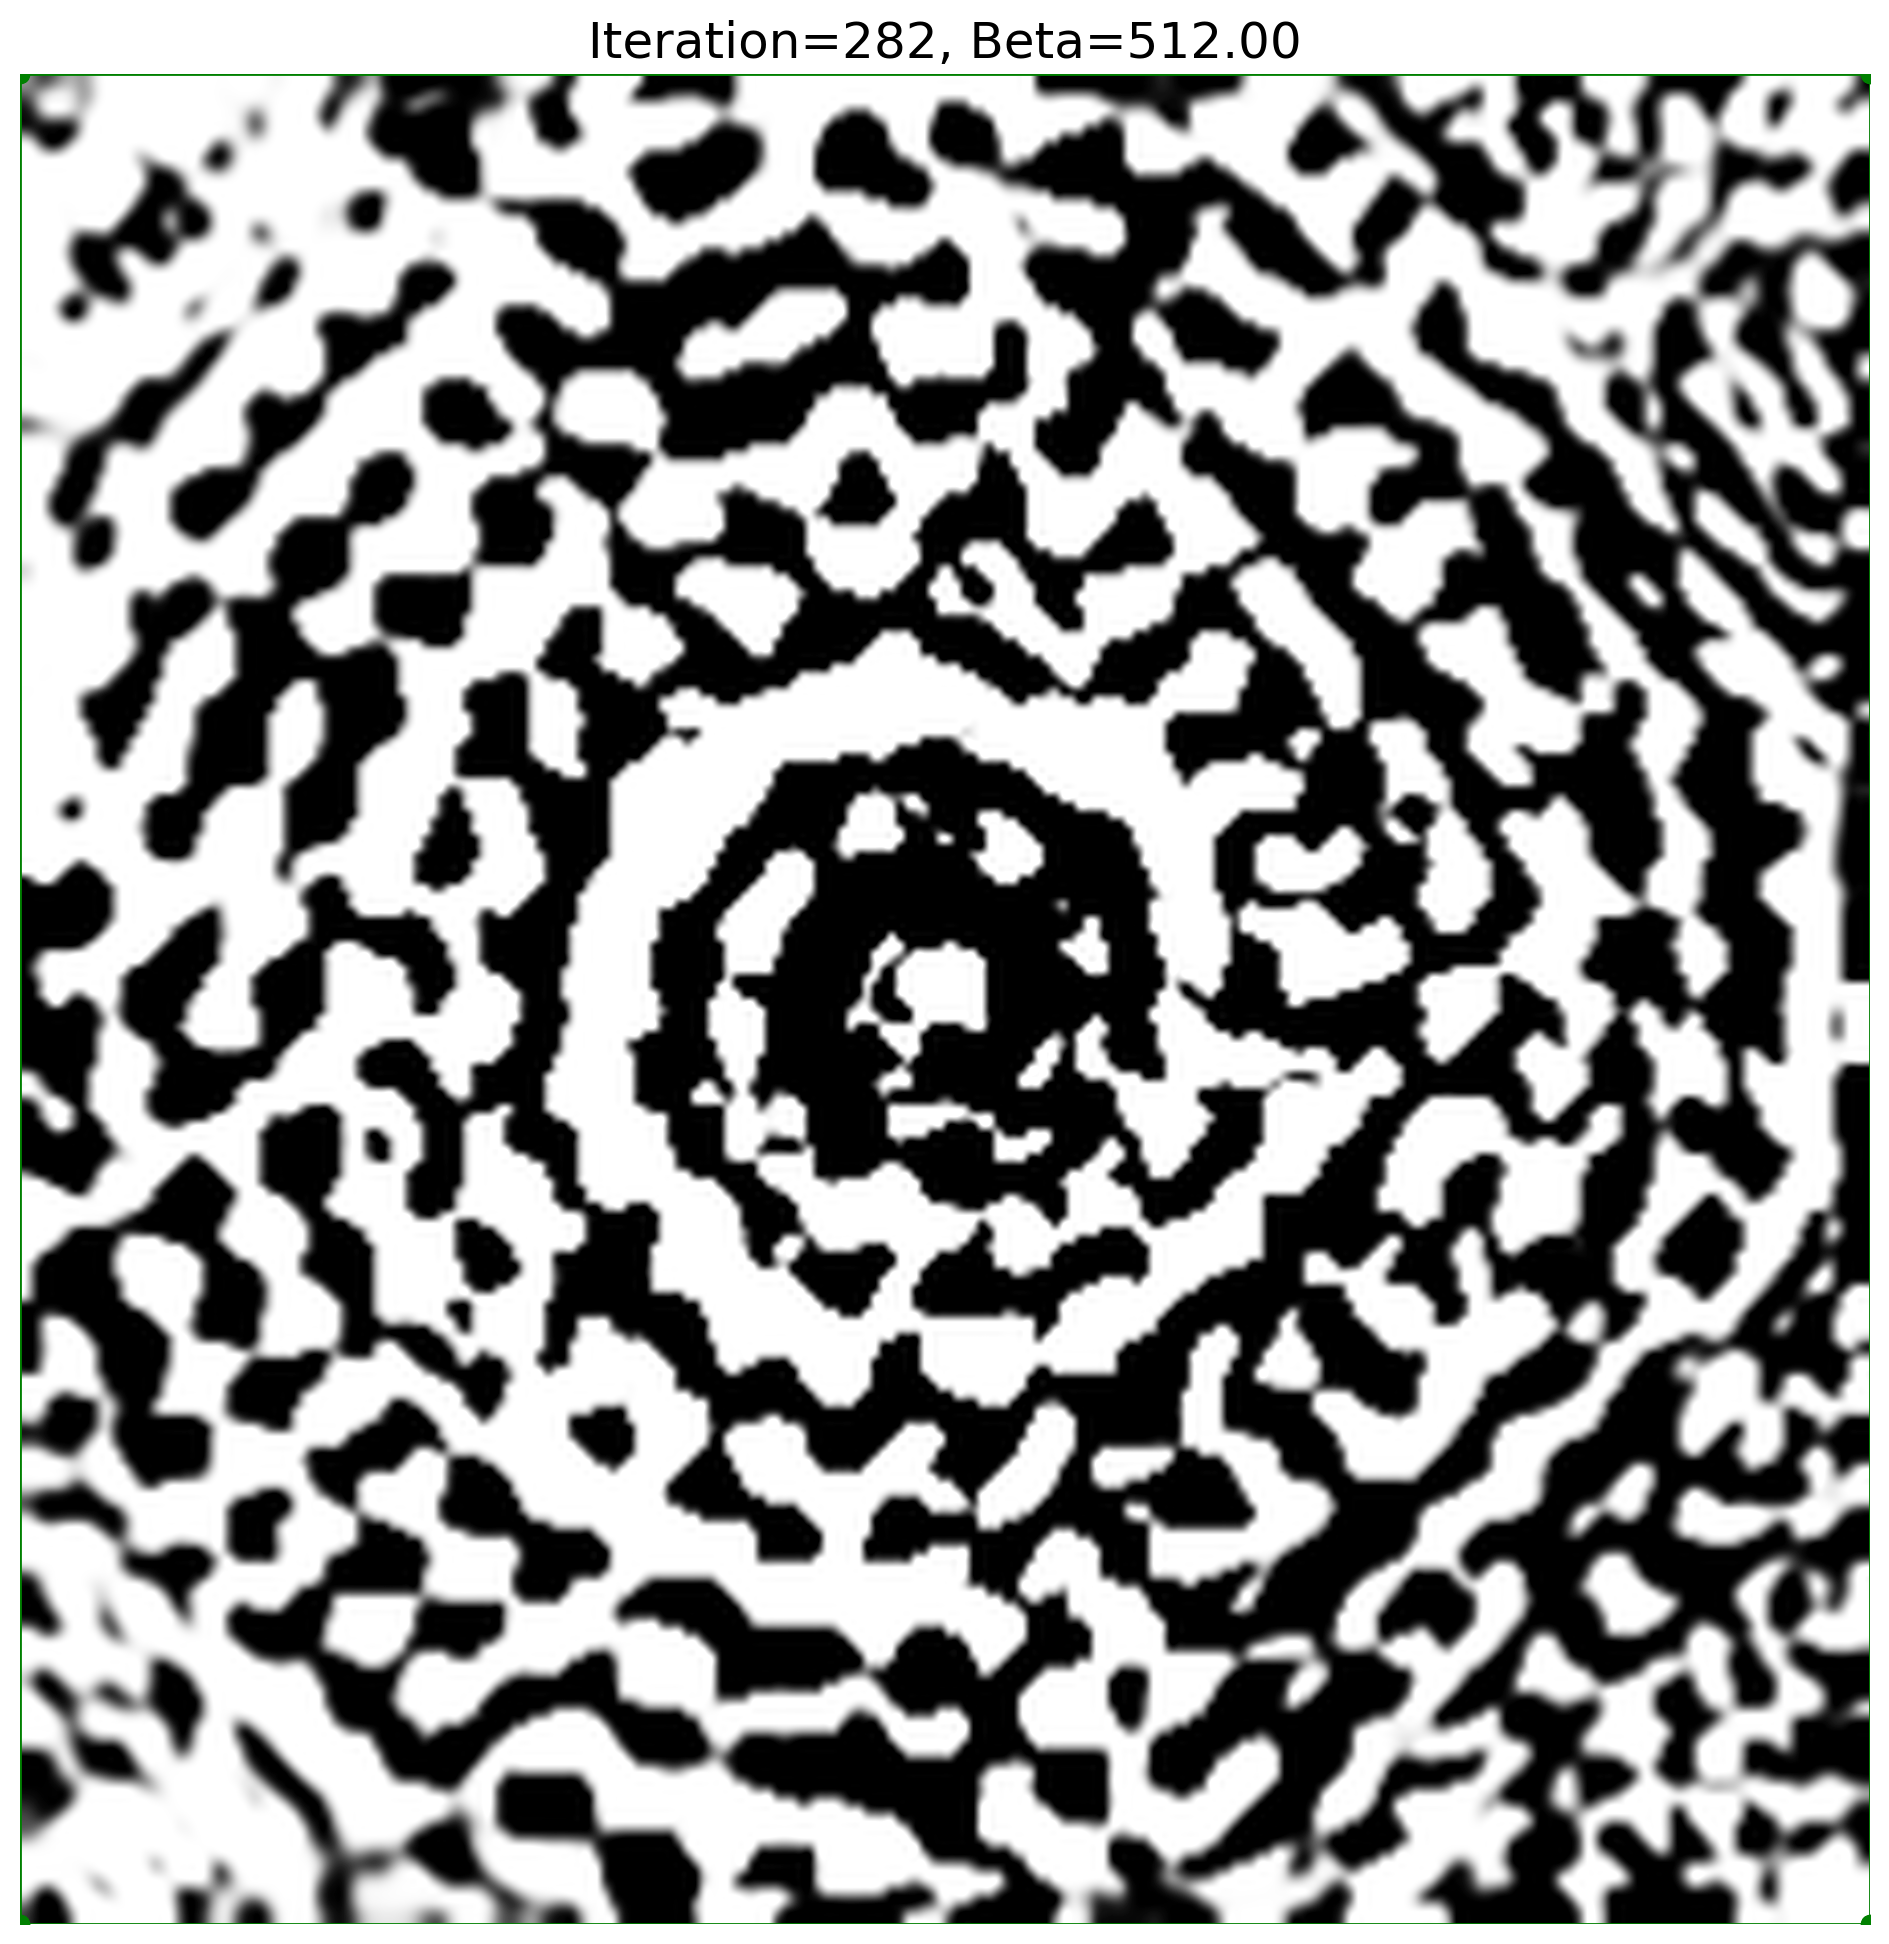
\includegraphics[width=0.3\textwidth]{img/018_structure_iter_282_beta_512.00.png} &
        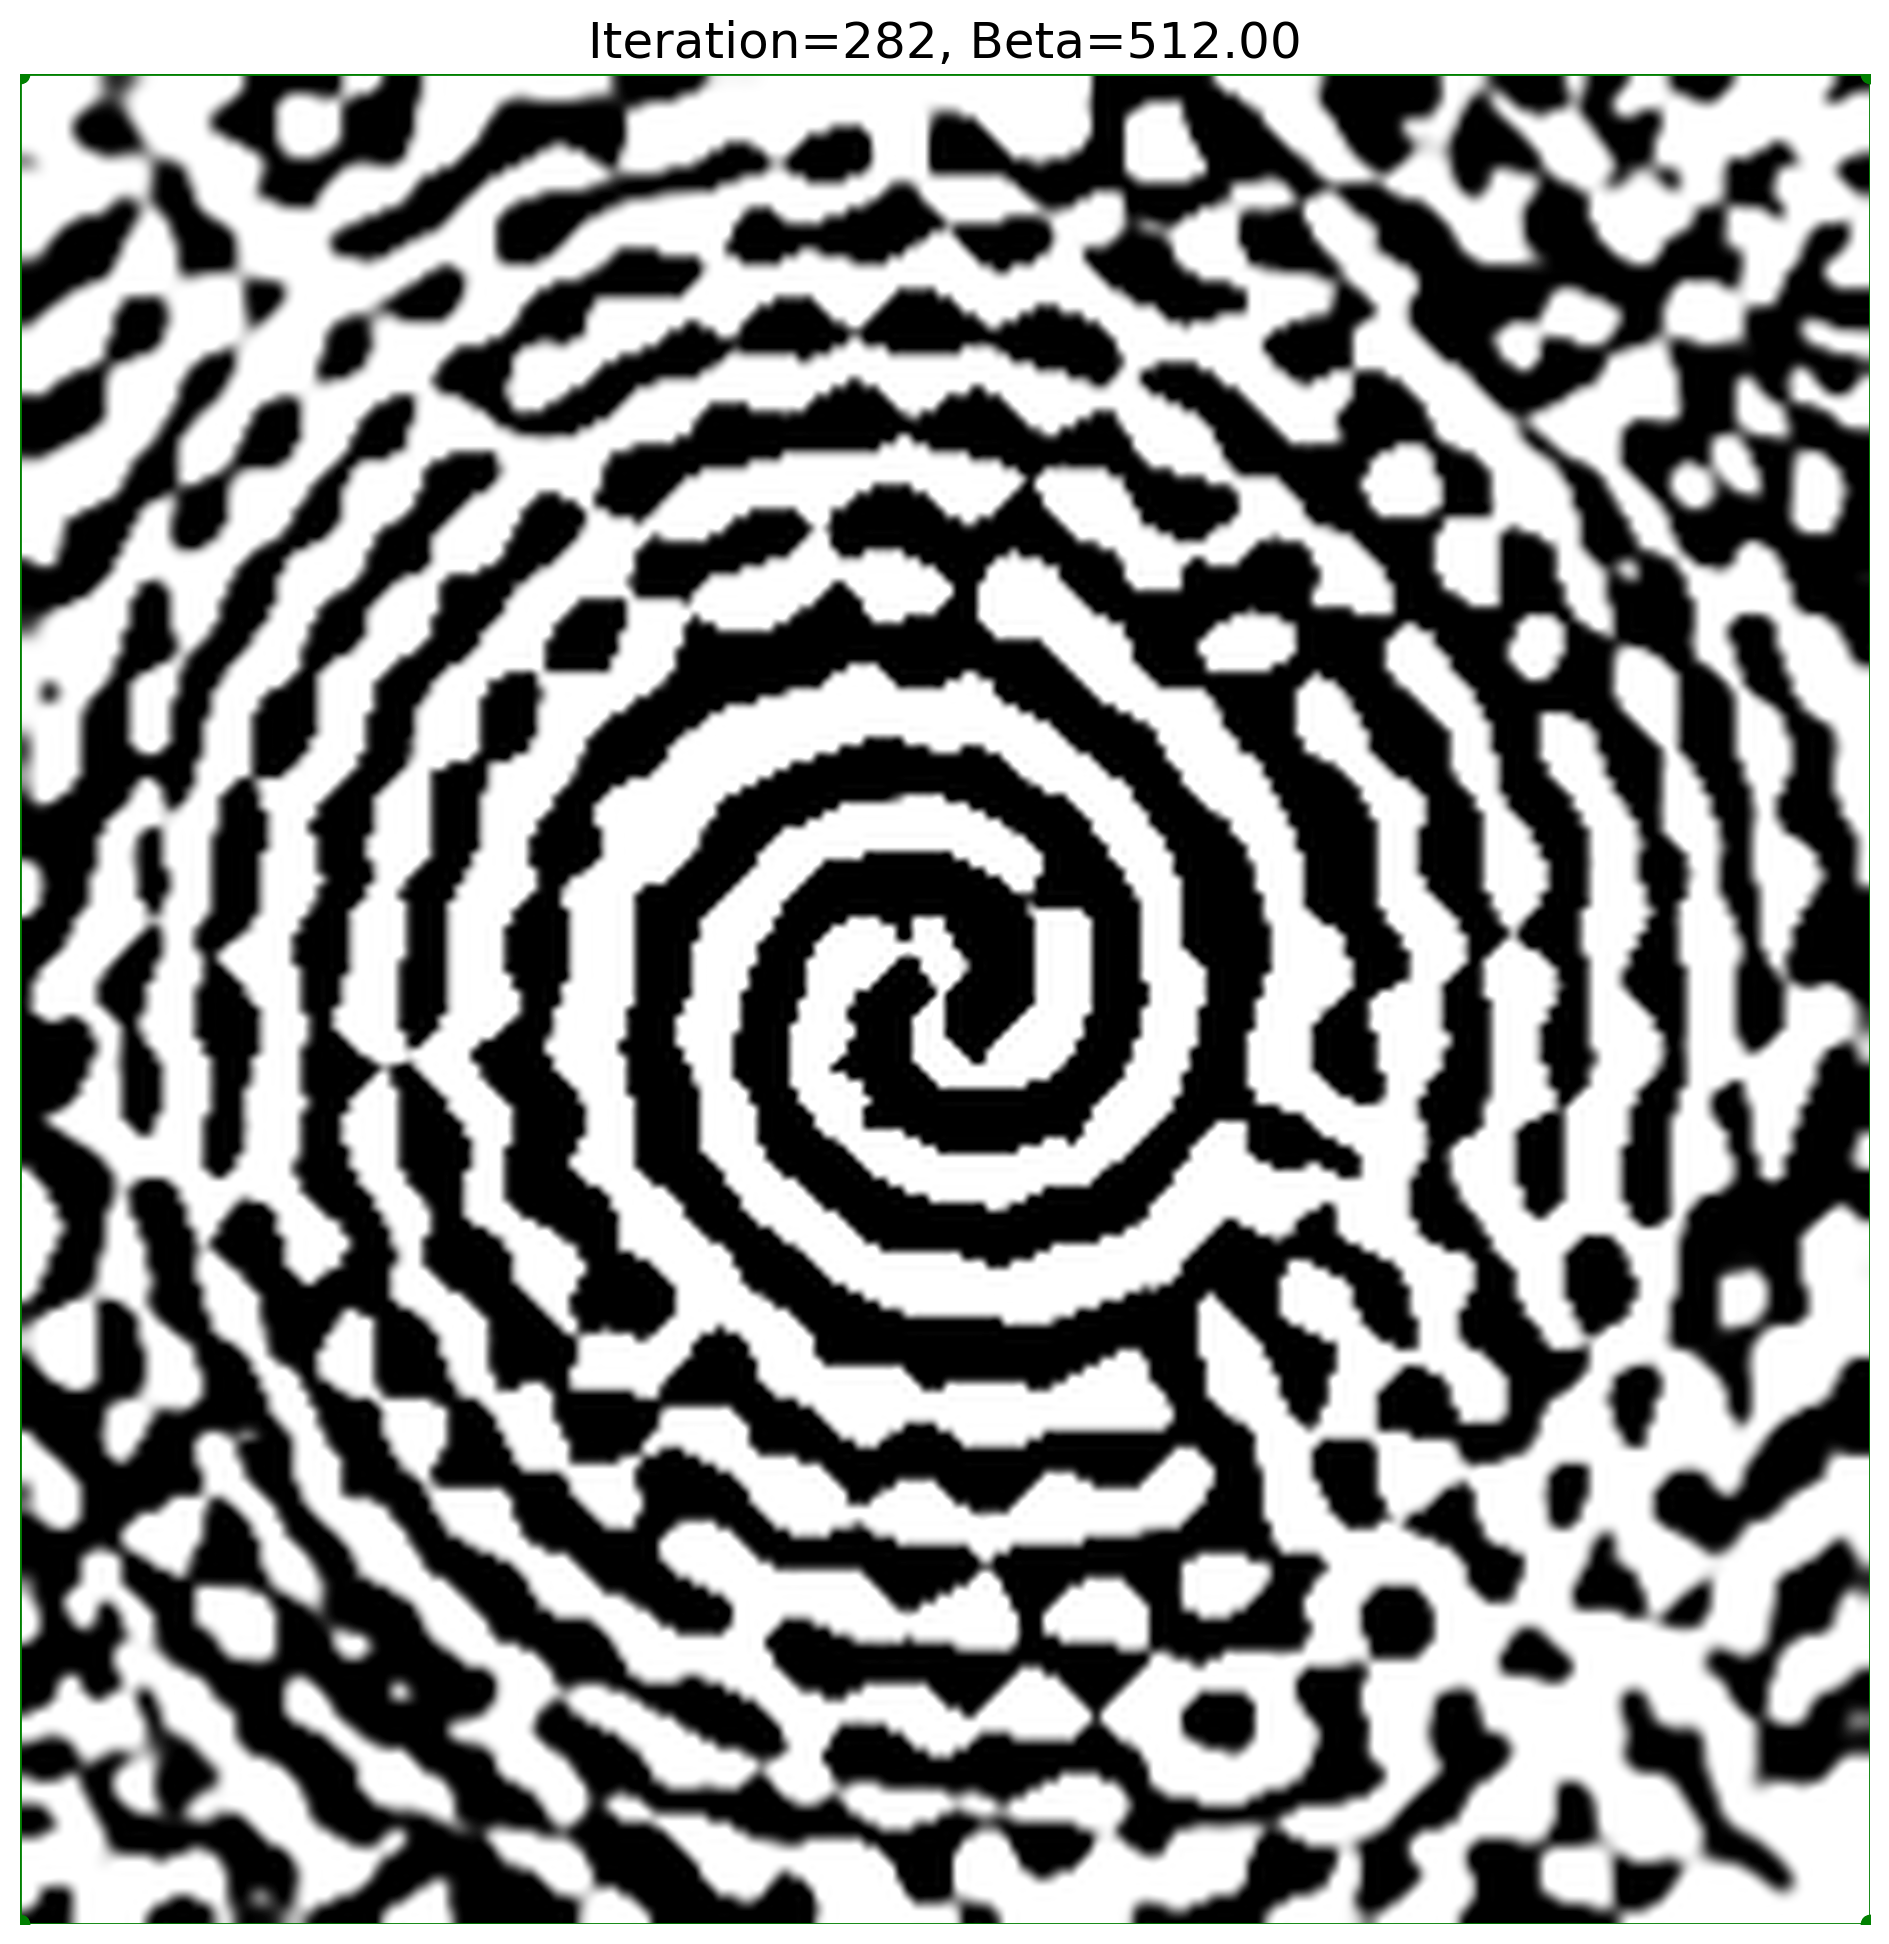
\includegraphics[width=0.3\textwidth]{img/013_structure_iter_282_beta_512.00.png} 
        \\ (a)  &  (b)  &  (c) \\[8pt]
        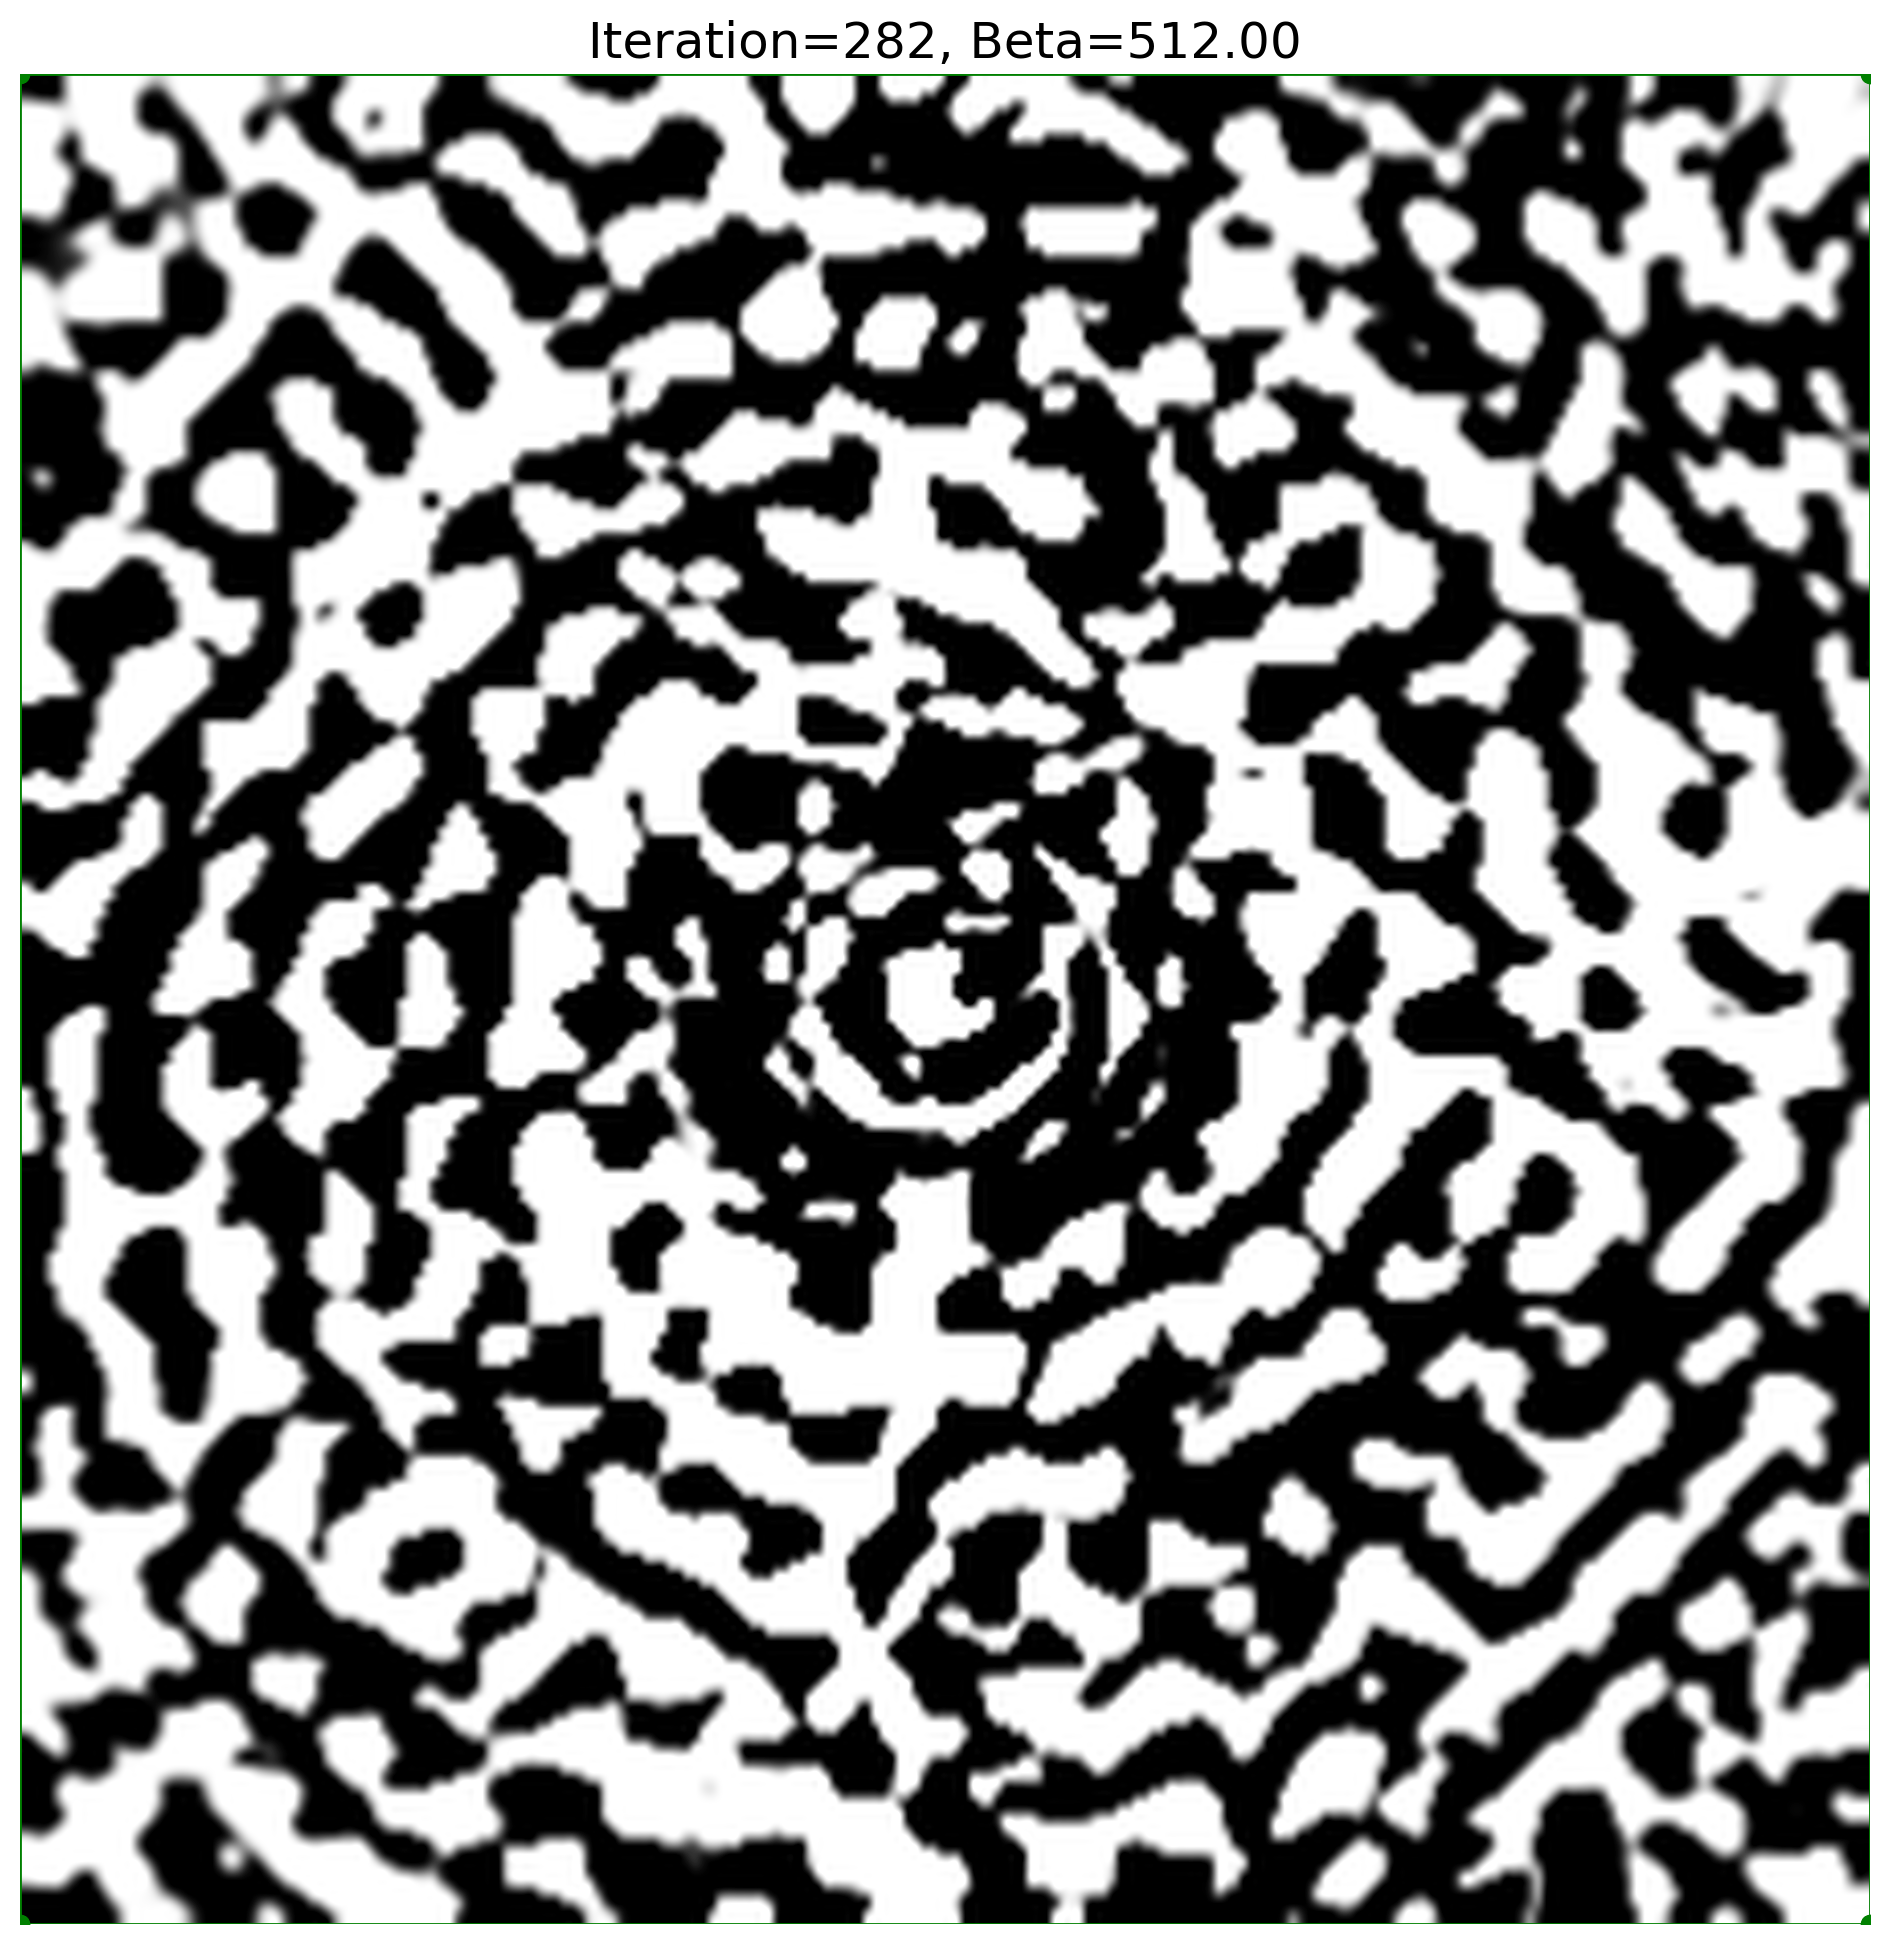
\includegraphics[width=0.3\textwidth]{img/020_structure_iter_282_beta_512.00.png} &
        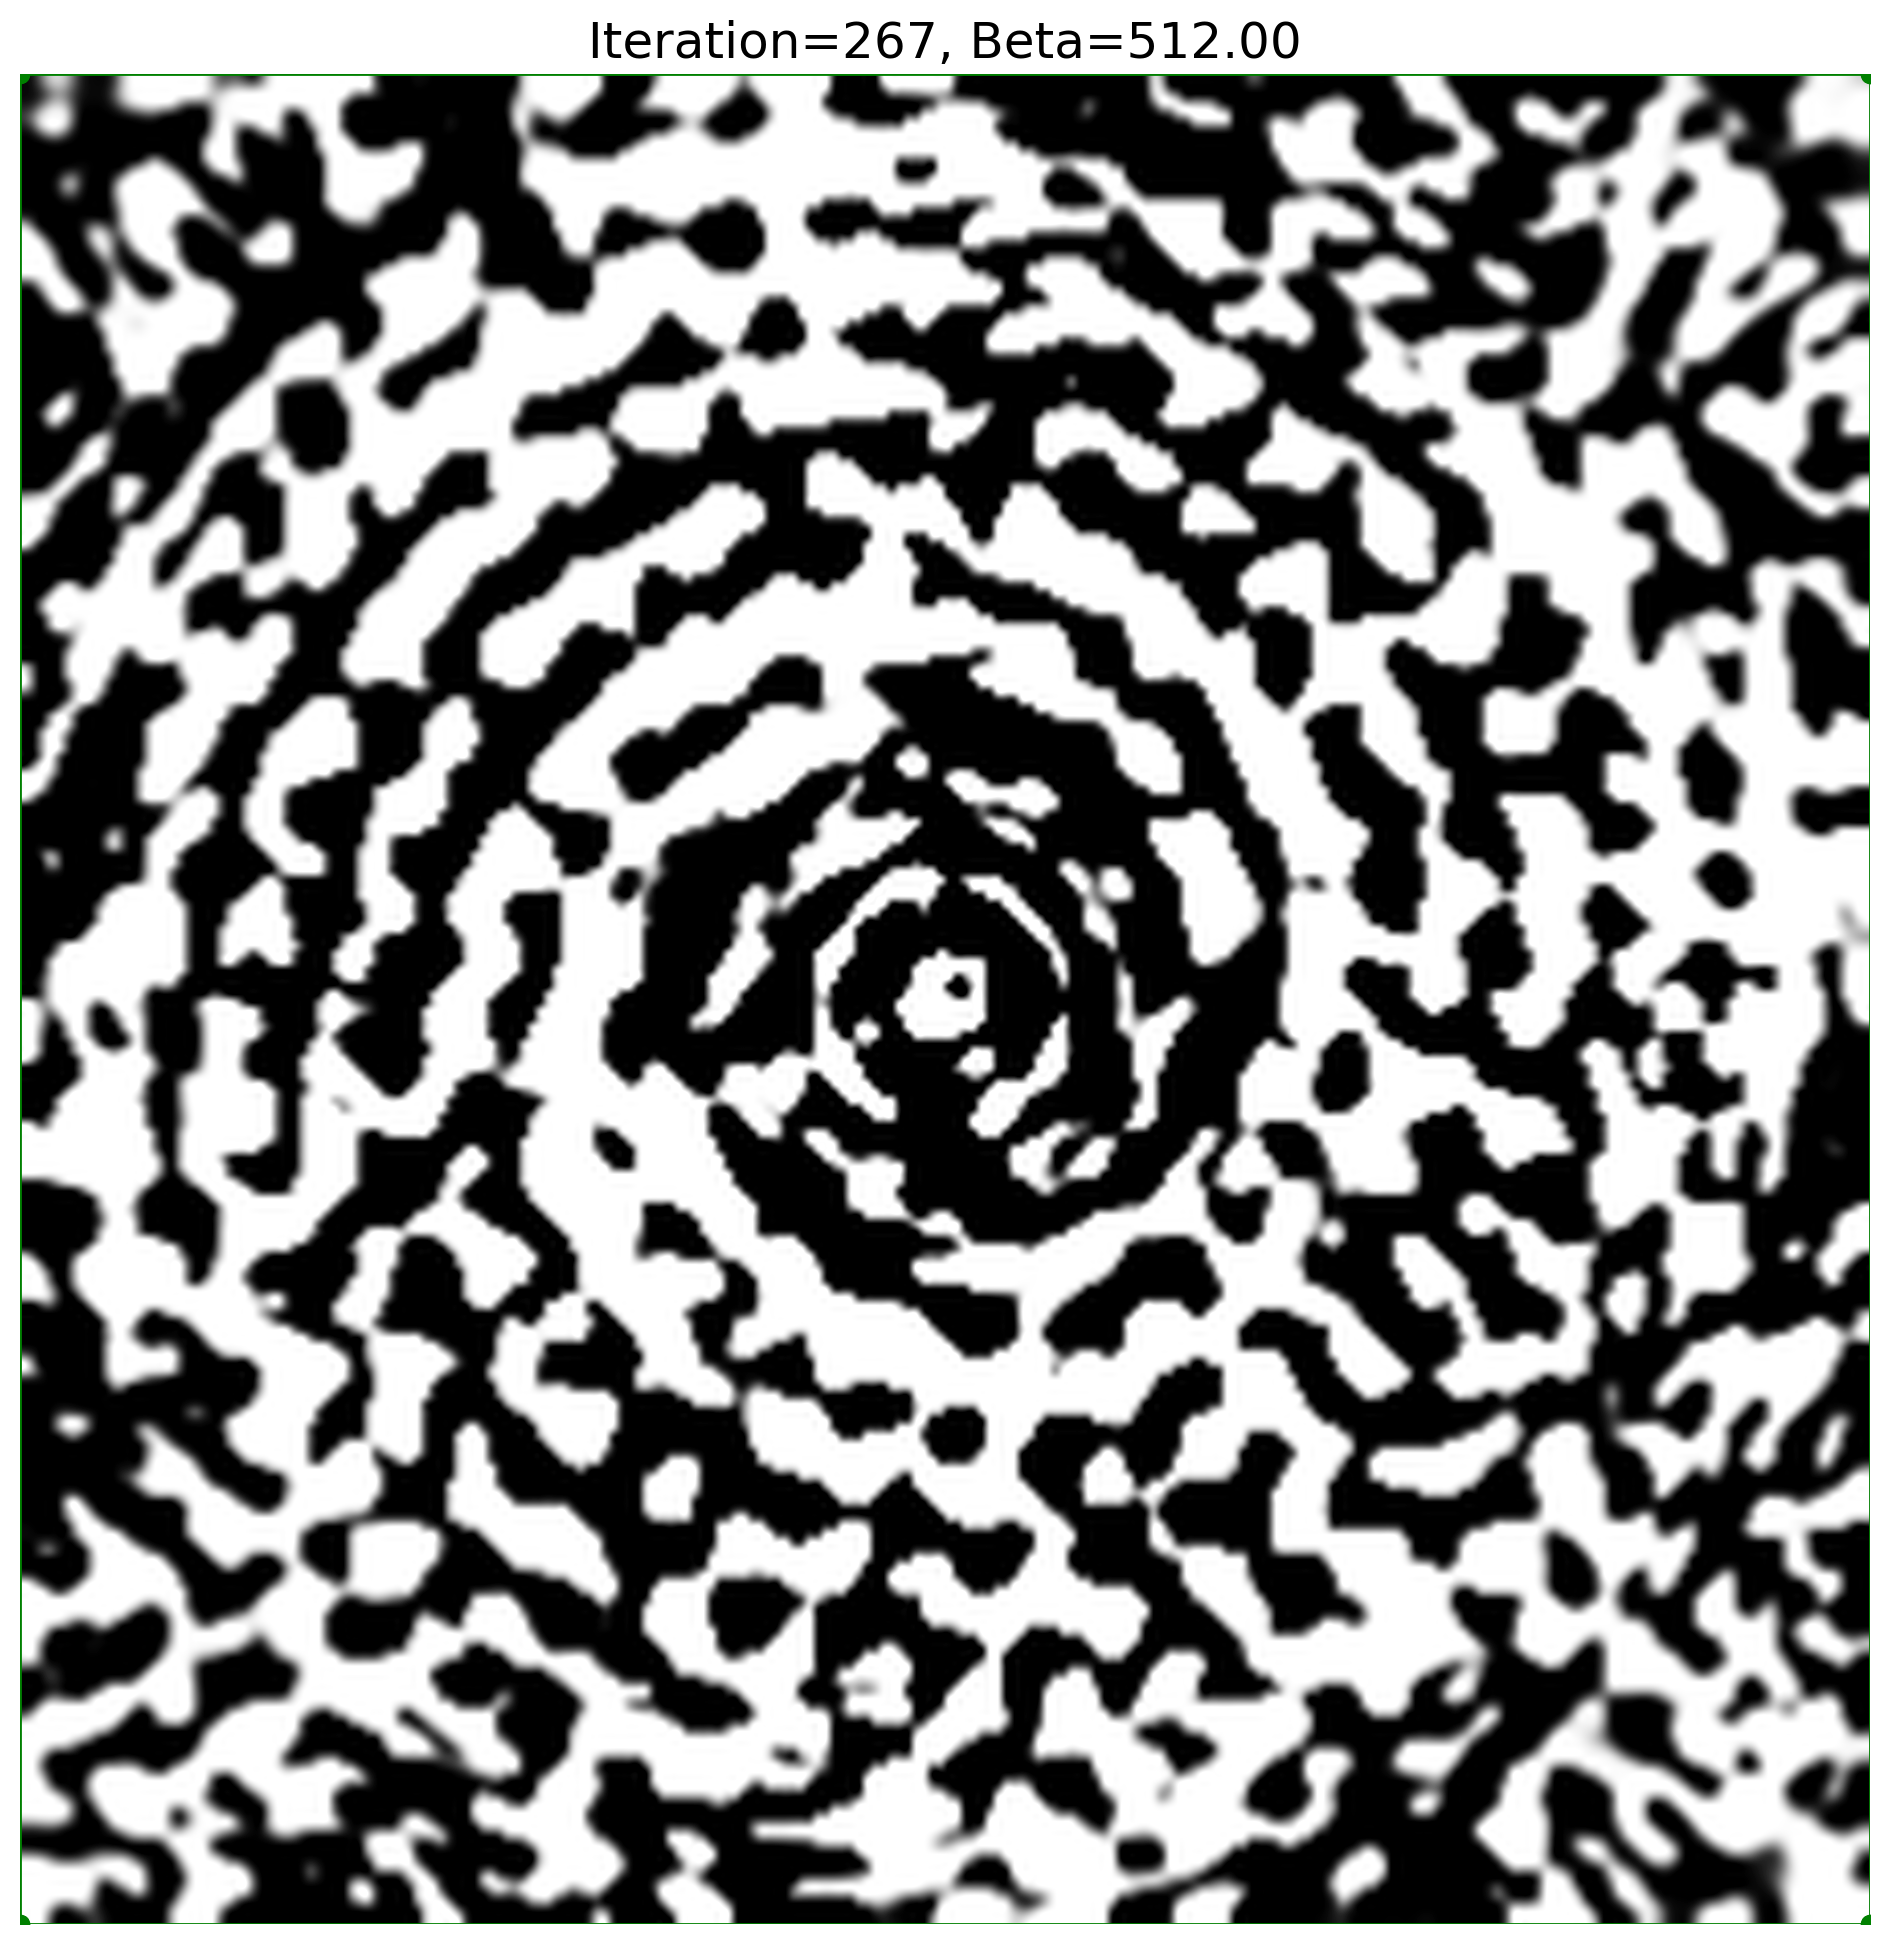
\includegraphics[width=0.3\textwidth]{img/021_structure_iter_267_beta_512.00.png} &
        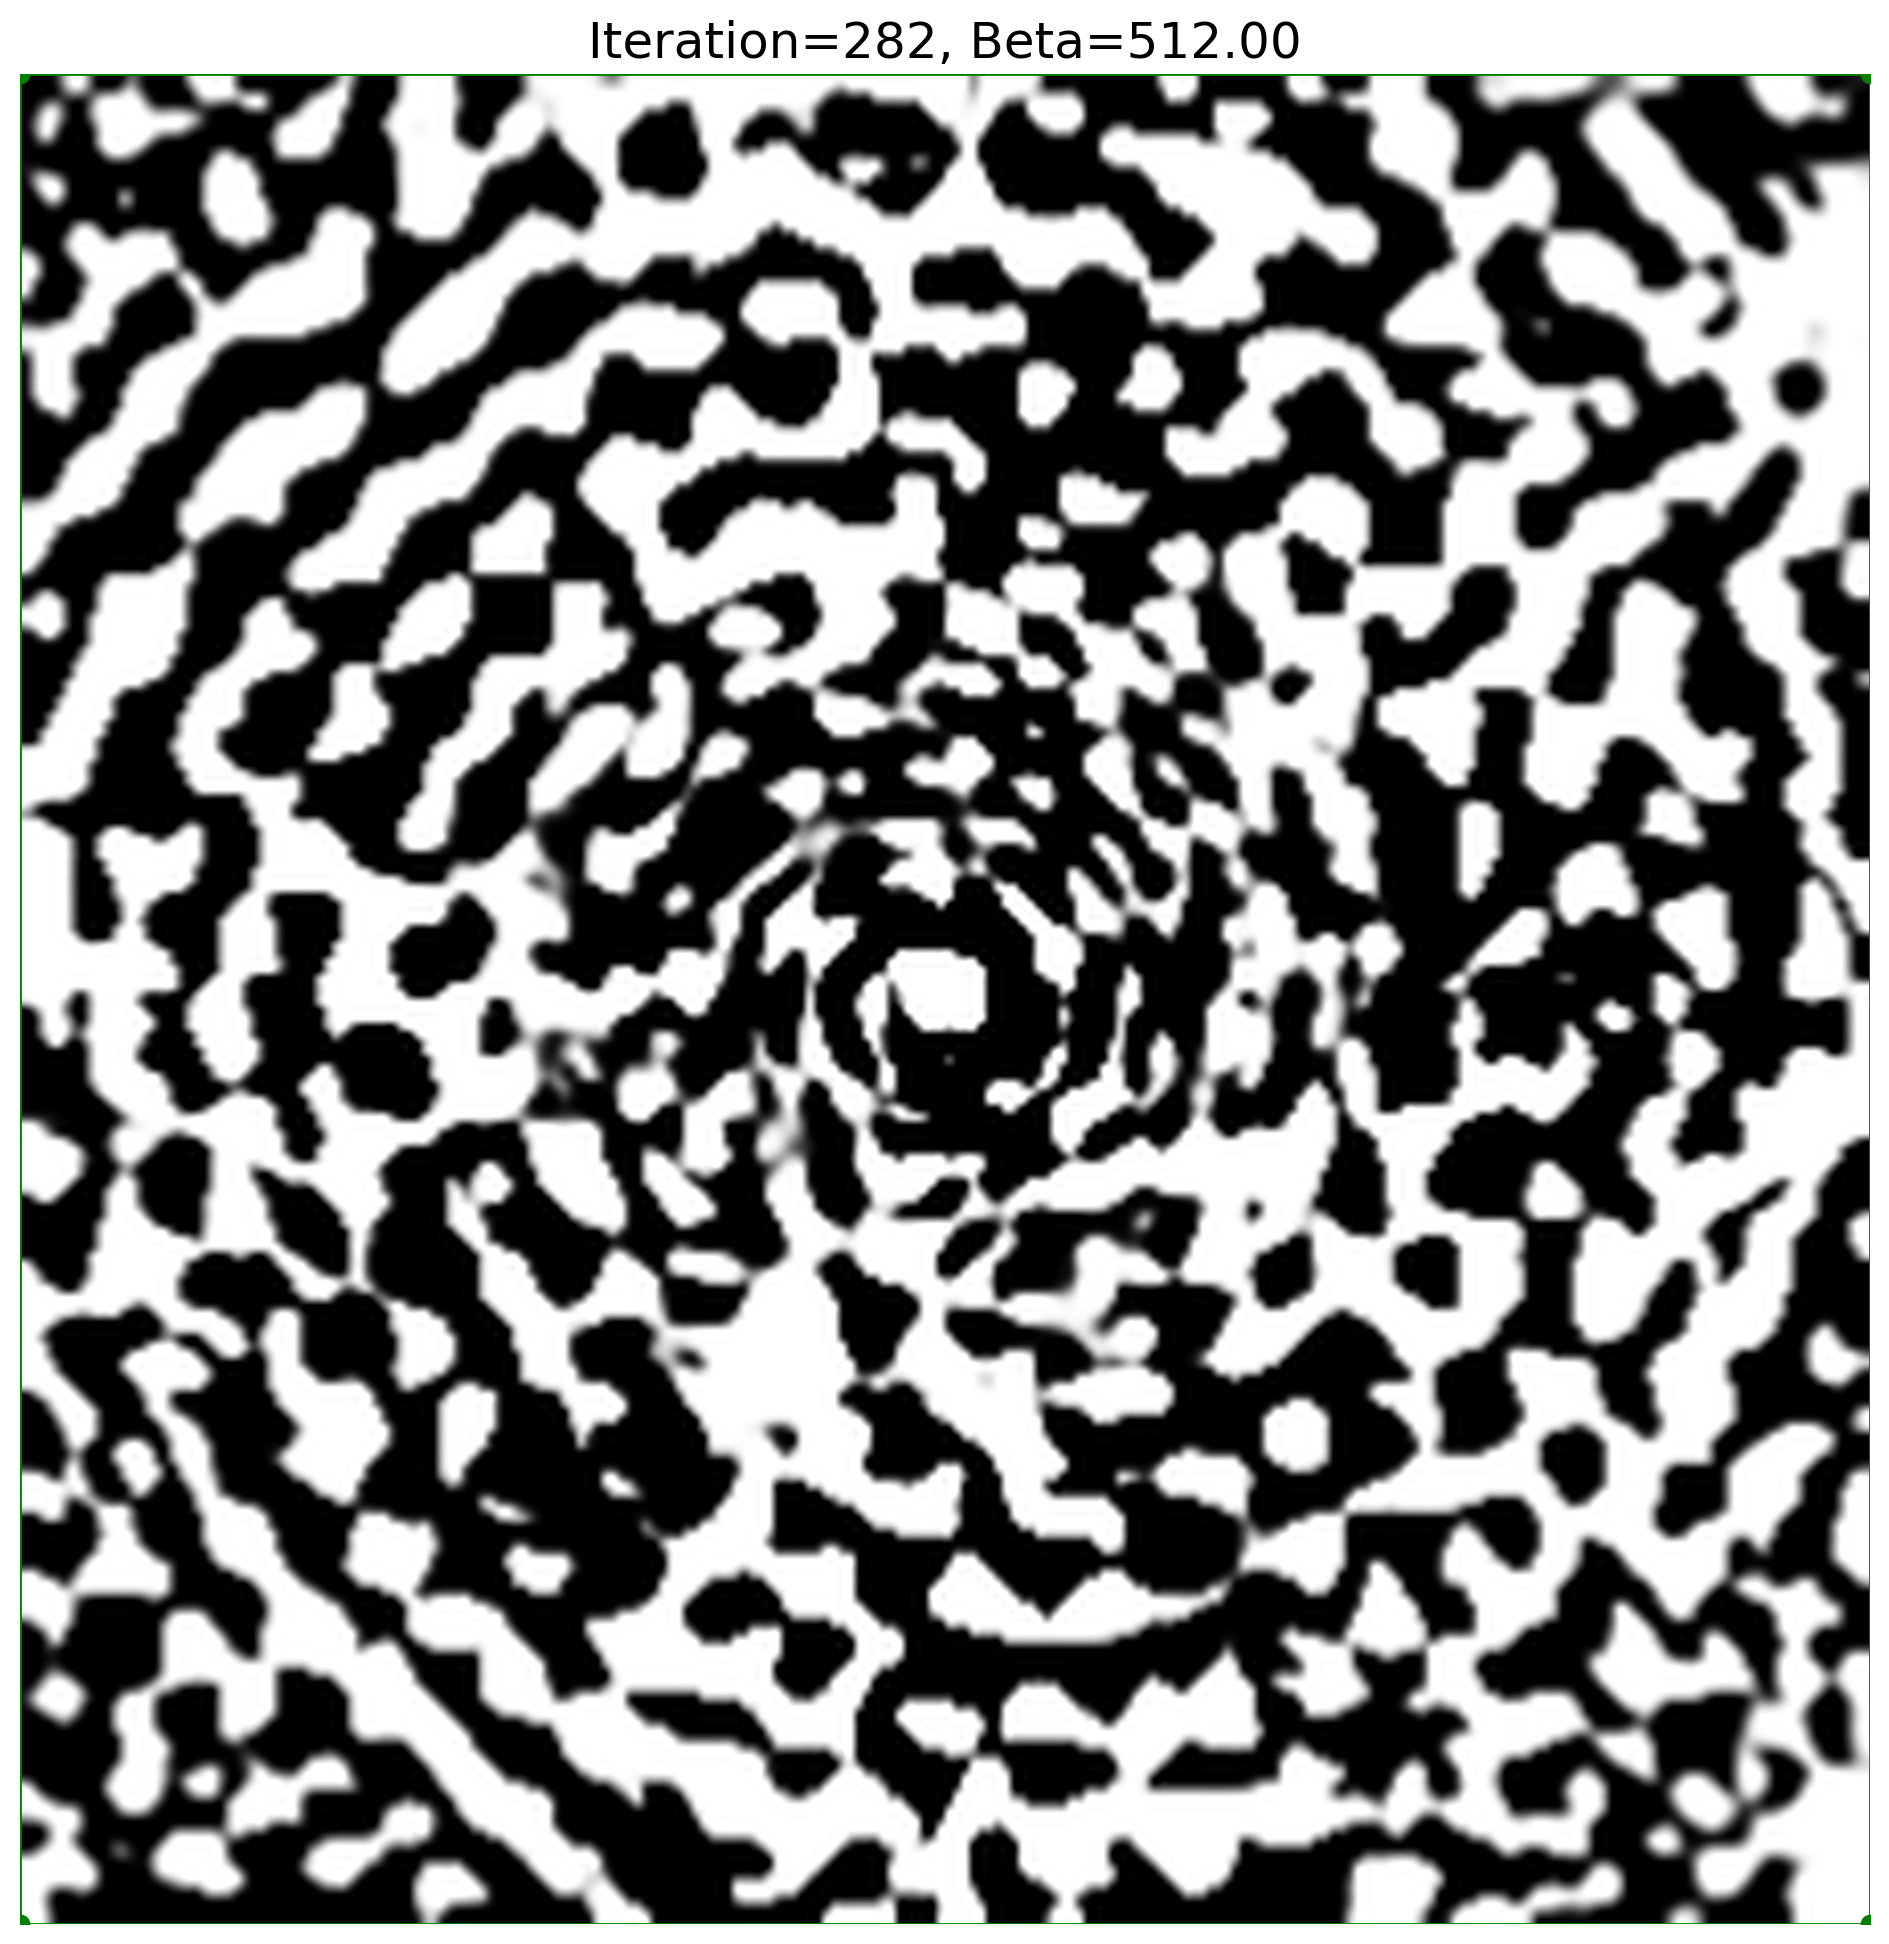
\includegraphics[width=0.3\textwidth]{img/022_structure_iter_282_beta_512.00.png}
        \\(d)  &  (e)  &  (f) 
    \end{tabular}
\caption{Final converged GaP/air binary material density distributions ($\beta = 512$, binarized structures): (a)$\sim$(f) $\ell \in \{0, 1, 2, 3, 4, 5\}$, respectively . Black represents GaP ($n = 3.31$); white represents air ($n = 1$). The $\ell = 2$ design shows a clear two-arm spiral pattern at the center, similar to a spiral phase plate (SPP). The other designs show free-form non-intuitive material distributions that do not follow simple $\ell$-fold rotational symmetry.}
\label{fig:structures_all}

\end{figure}


%===================================================================

\section{Near-Field Characteristics}

\label{sec:nearfield}

Figure~\ref{fig:nearfield_all} shows the LCP and RCP electric field phase and normalized intensity distributions ($|E_\text{LCP}|^2$ and $|E_\text{RCP}|^2$) at the near-field monitor plane just above the design layer for the six designs.

The LCP intensity distribution (upper right of each group) is concentrated in the central region of the structure ($\sim 1\;\mu\text{m}$ scale) for all designs, showing non-uniform localized enhancement that reflects the near-field collection efficiency of the optimized structure for LCP dipole radiation. The LCP phase distribution (upper left of each group) shows a complex spatial pattern due to structural scattering—a stark contrast to the ordered spiral phase in the far field—indicating that near-field phase modulation arises from the collective action of scattering effects rather than local phase delay.

The RCP component (bottom row of each group) has clearly lower intensity than the LCP component; the normalized intensity ratio between the two directly reflects the structure's circular polarization selectivity (see Section~\ref{sec:pol_selectivity}). The RCP intensity distribution pattern varies across designs but shows no concentrated near-field enhancement like LCP in any case, indicating that the optimized structure indeed exhibits selective near-field coupling to the K-valley LCP radiation.

\begin{figure}[htb]
\centering
	\begin{tabular}{cc} 
	    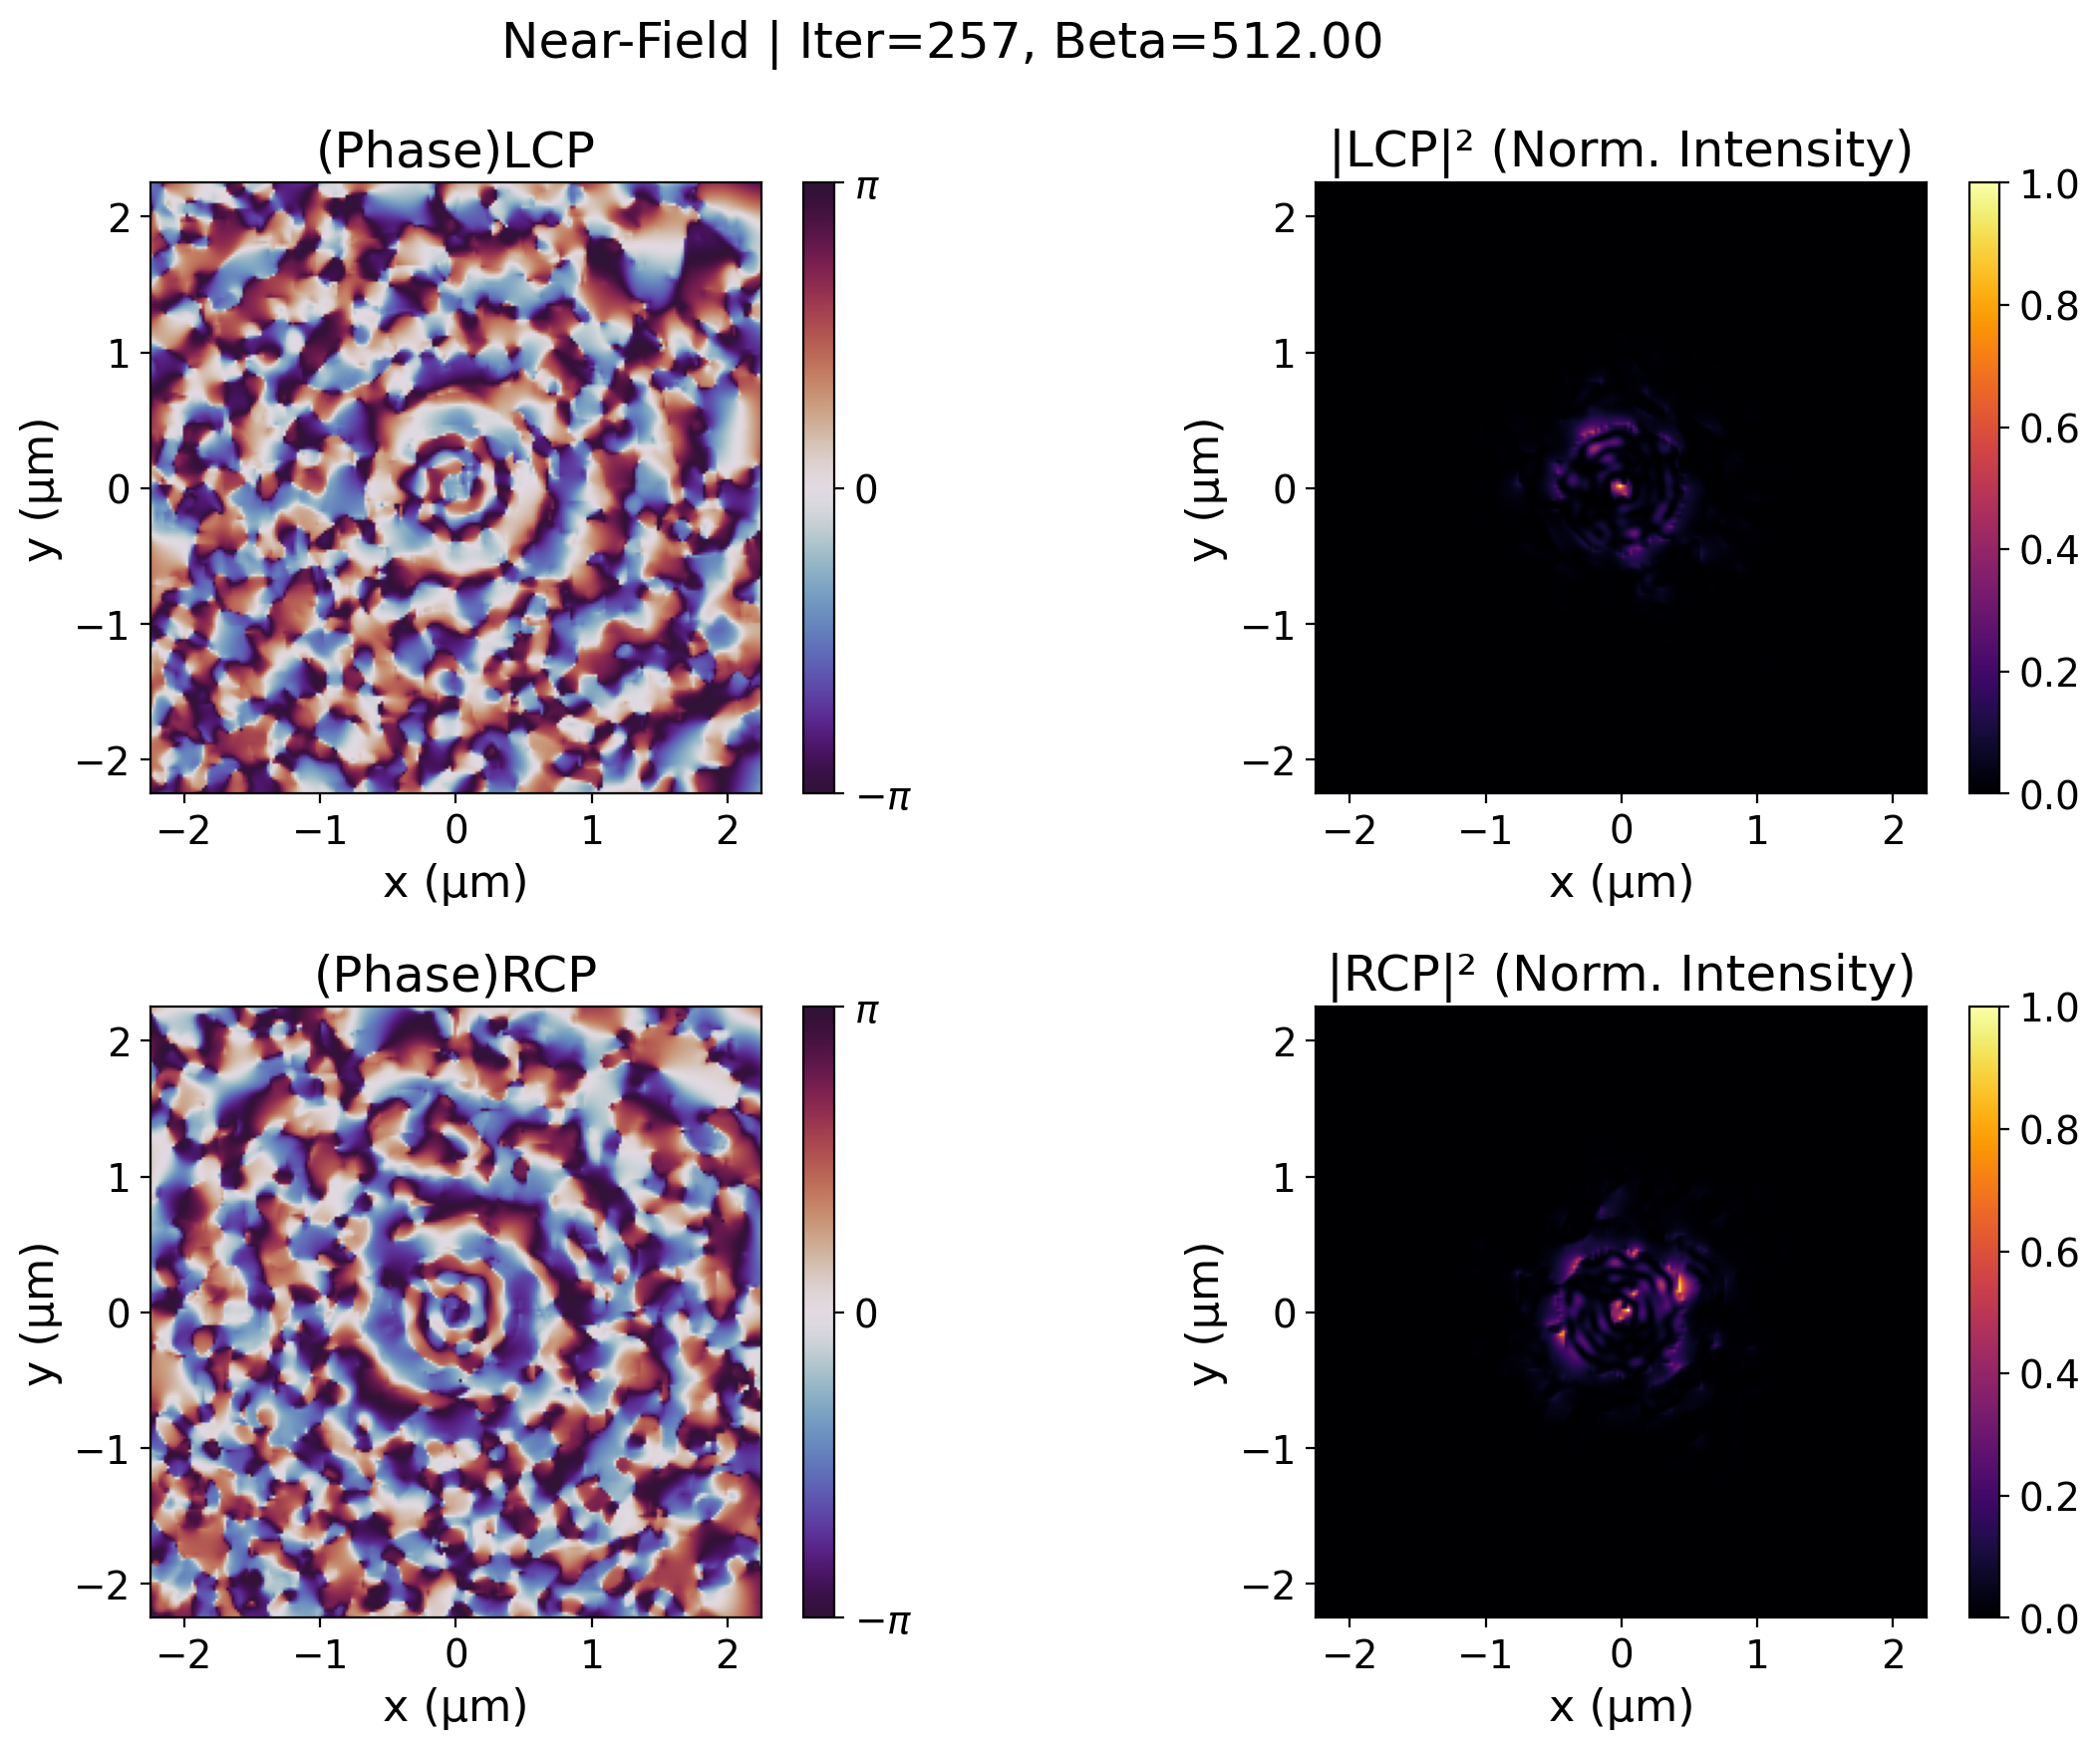
\includegraphics[width=0.47\textwidth]{img/017_phase_iter_257_beta_512.00.png}&
	    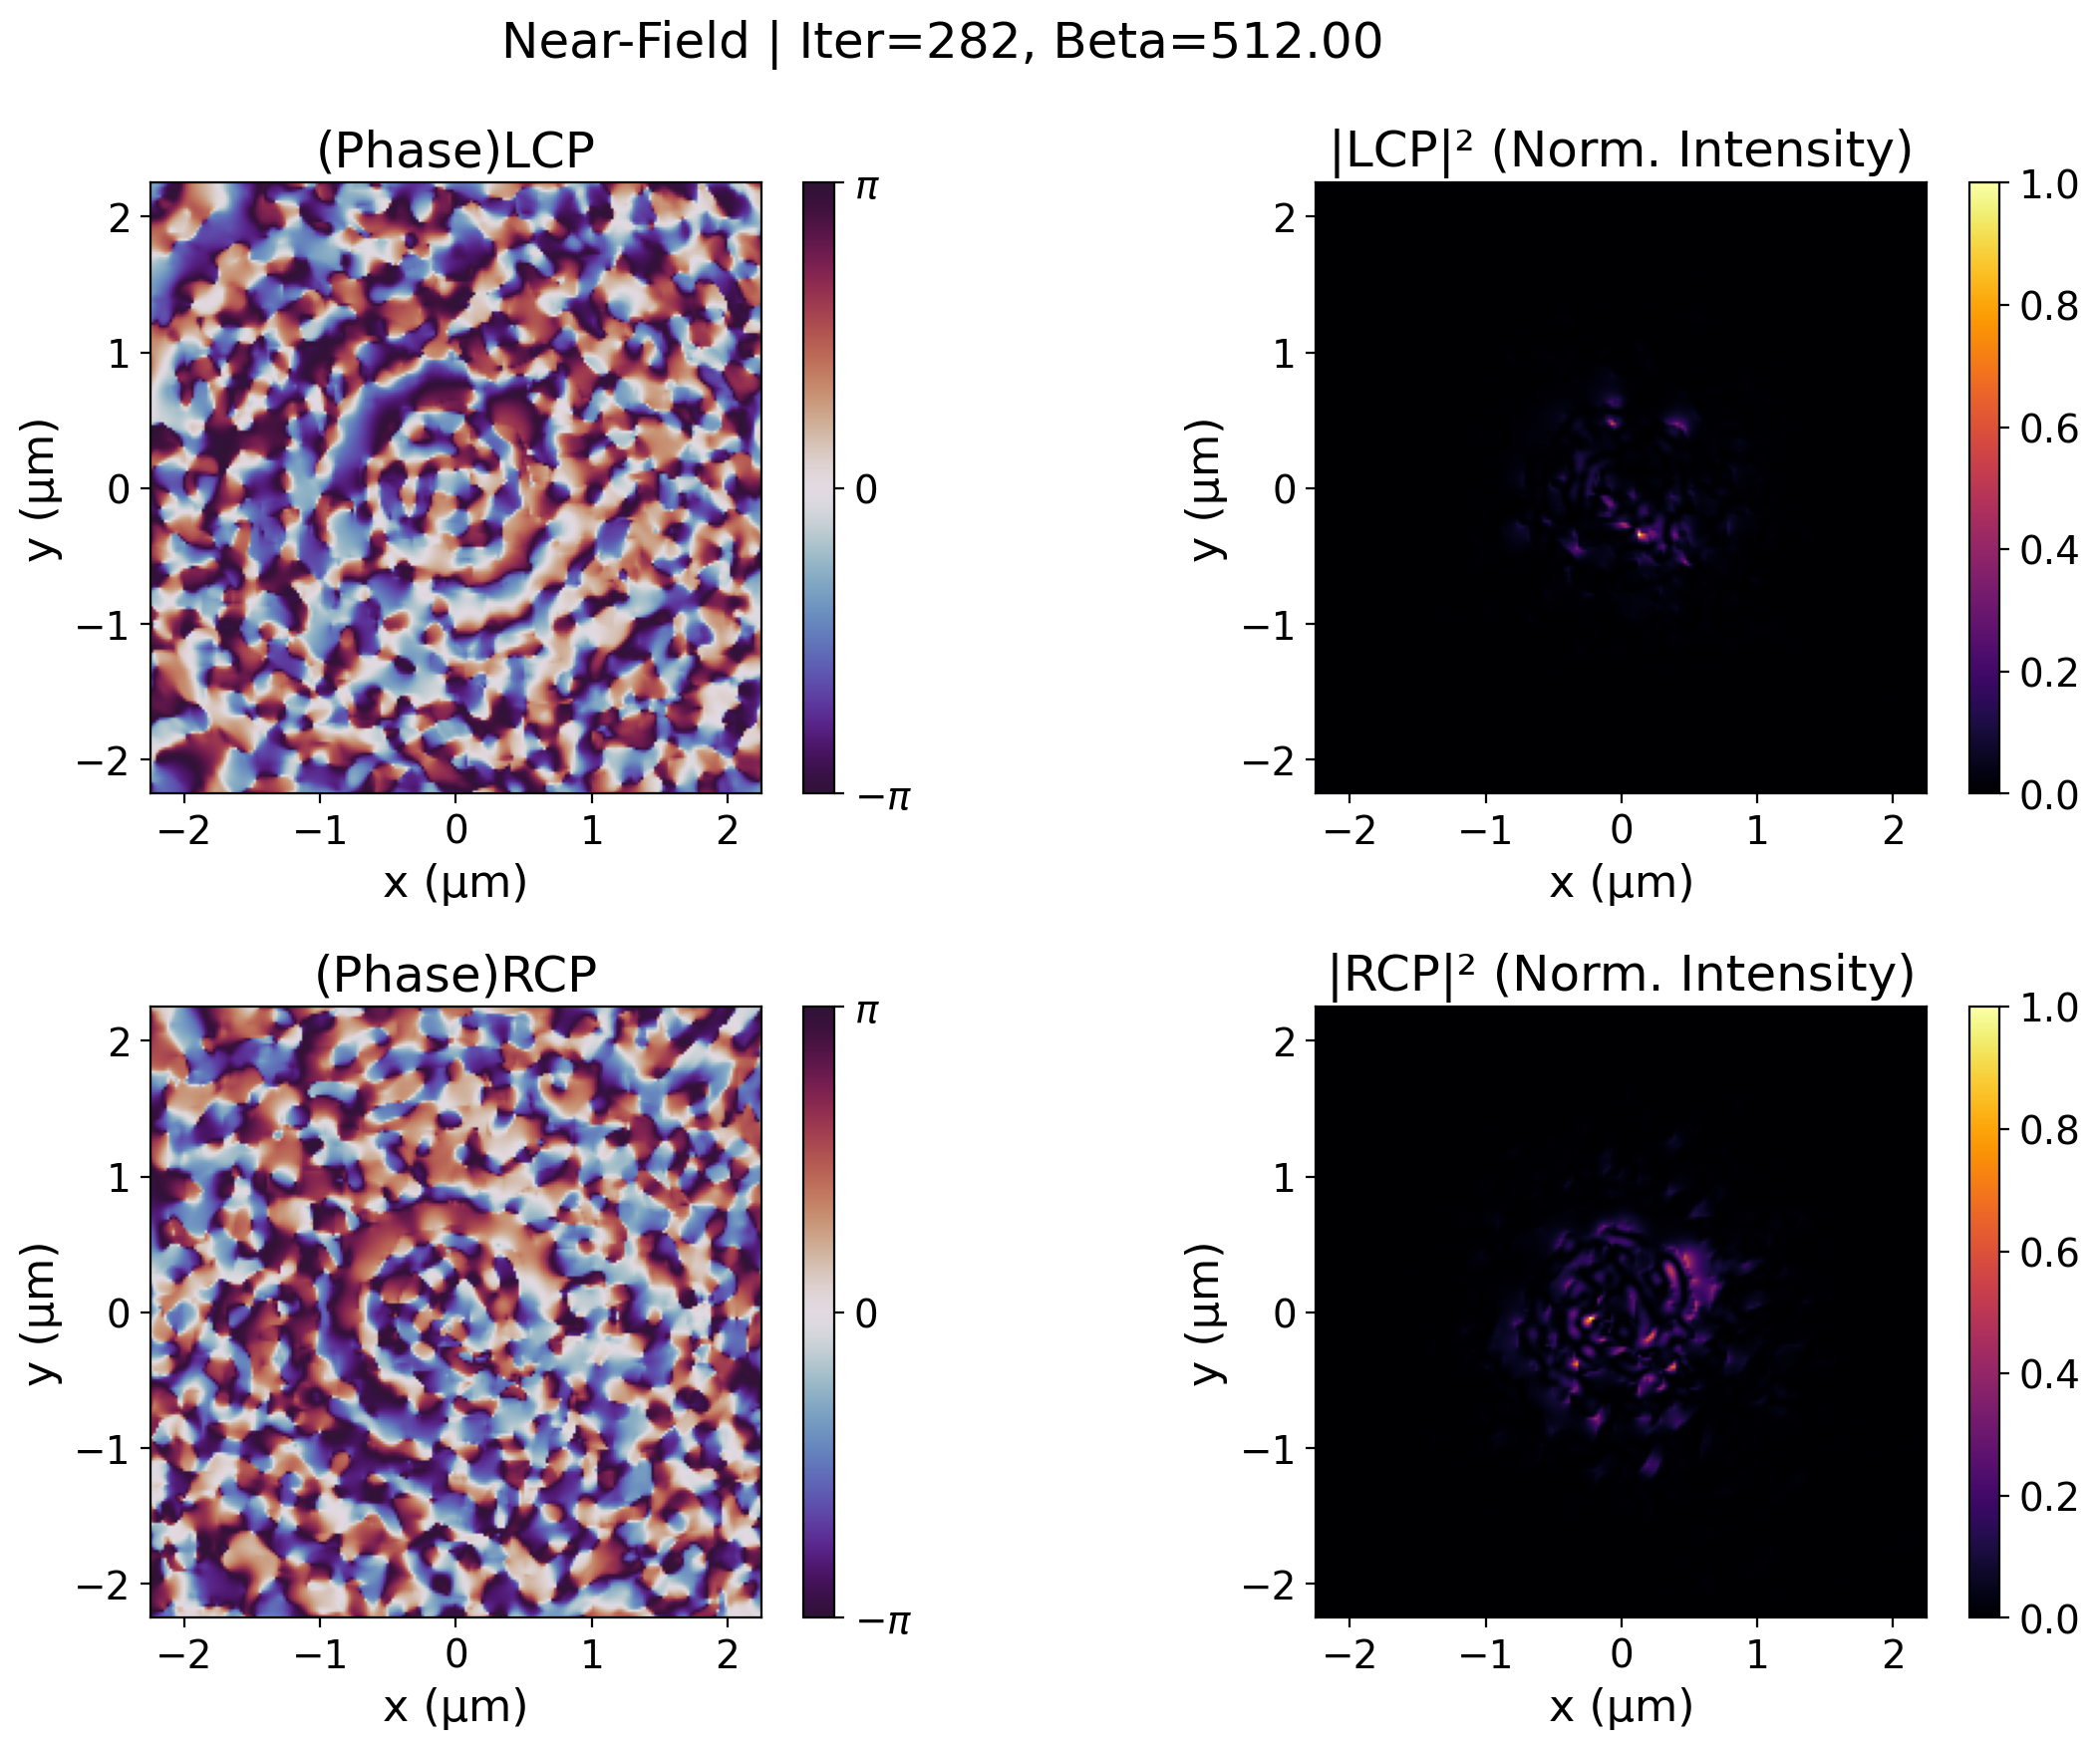
\includegraphics[width=0.47\textwidth]{img/018_phase_iter_282_beta_512.00.png}
		\\ (a)  & (b) \\[6pt]
		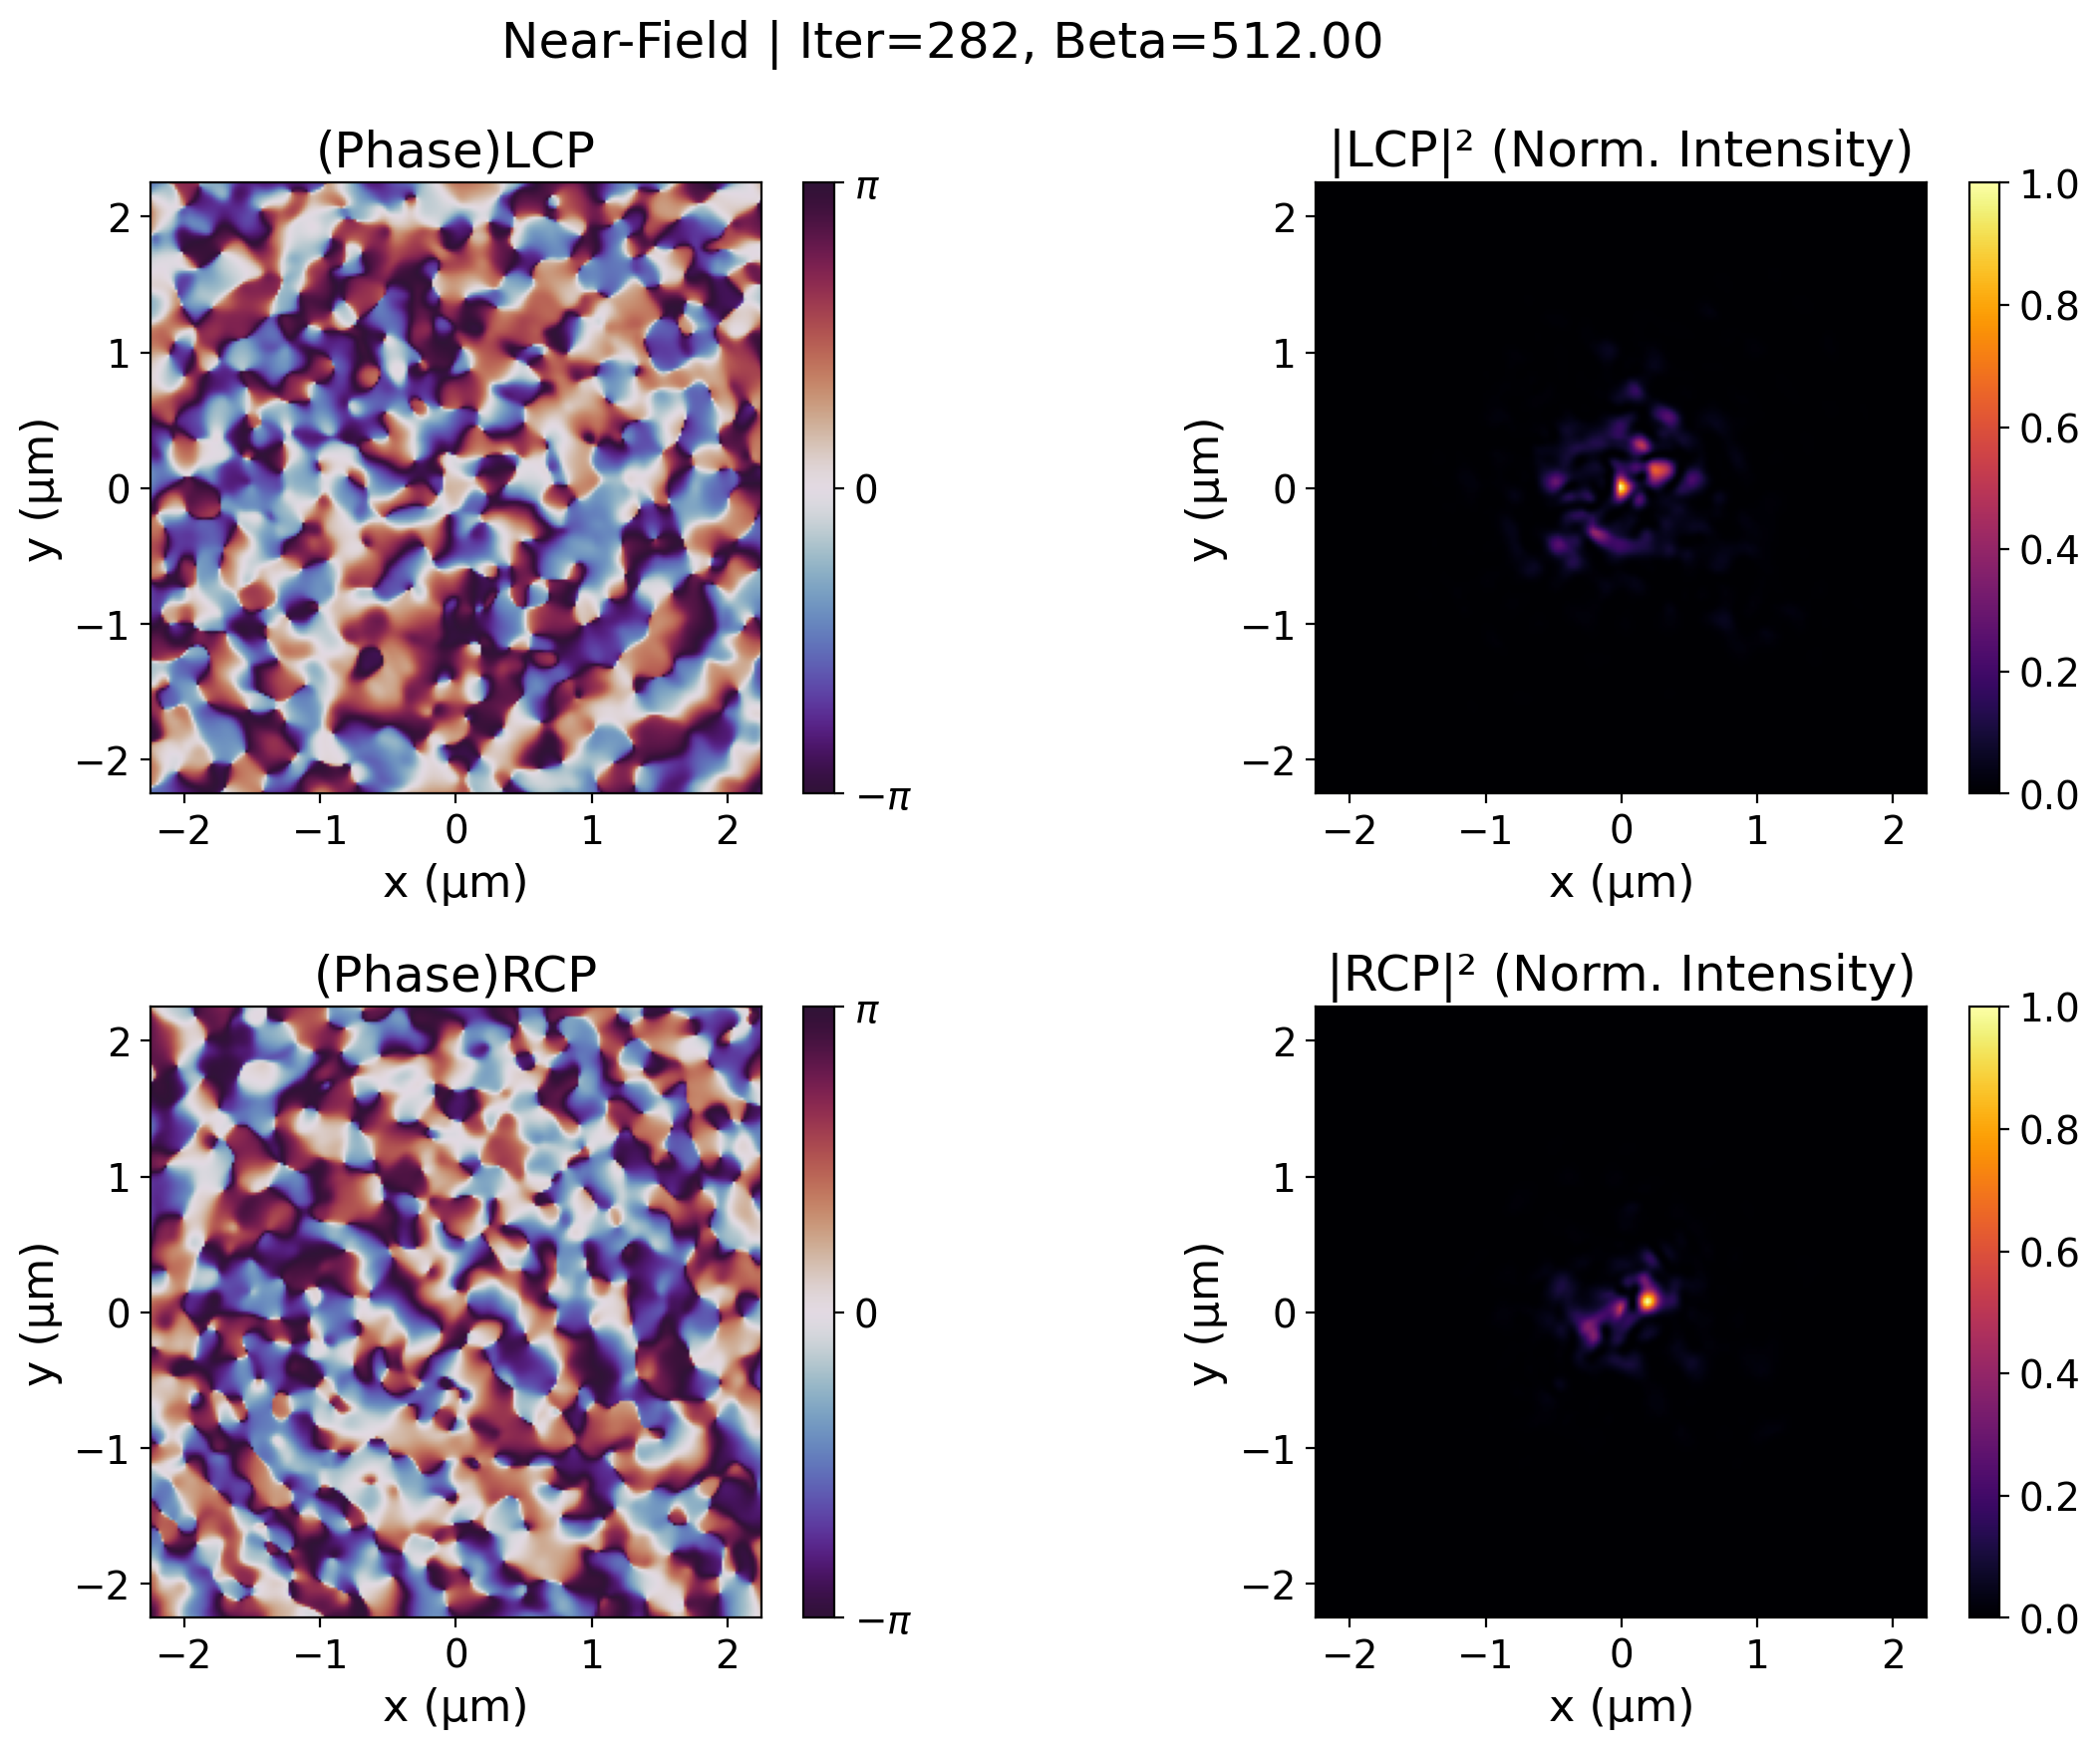
\includegraphics[width=0.47\textwidth]{img/013_phase_iter_282_beta_512.00.png}&
	    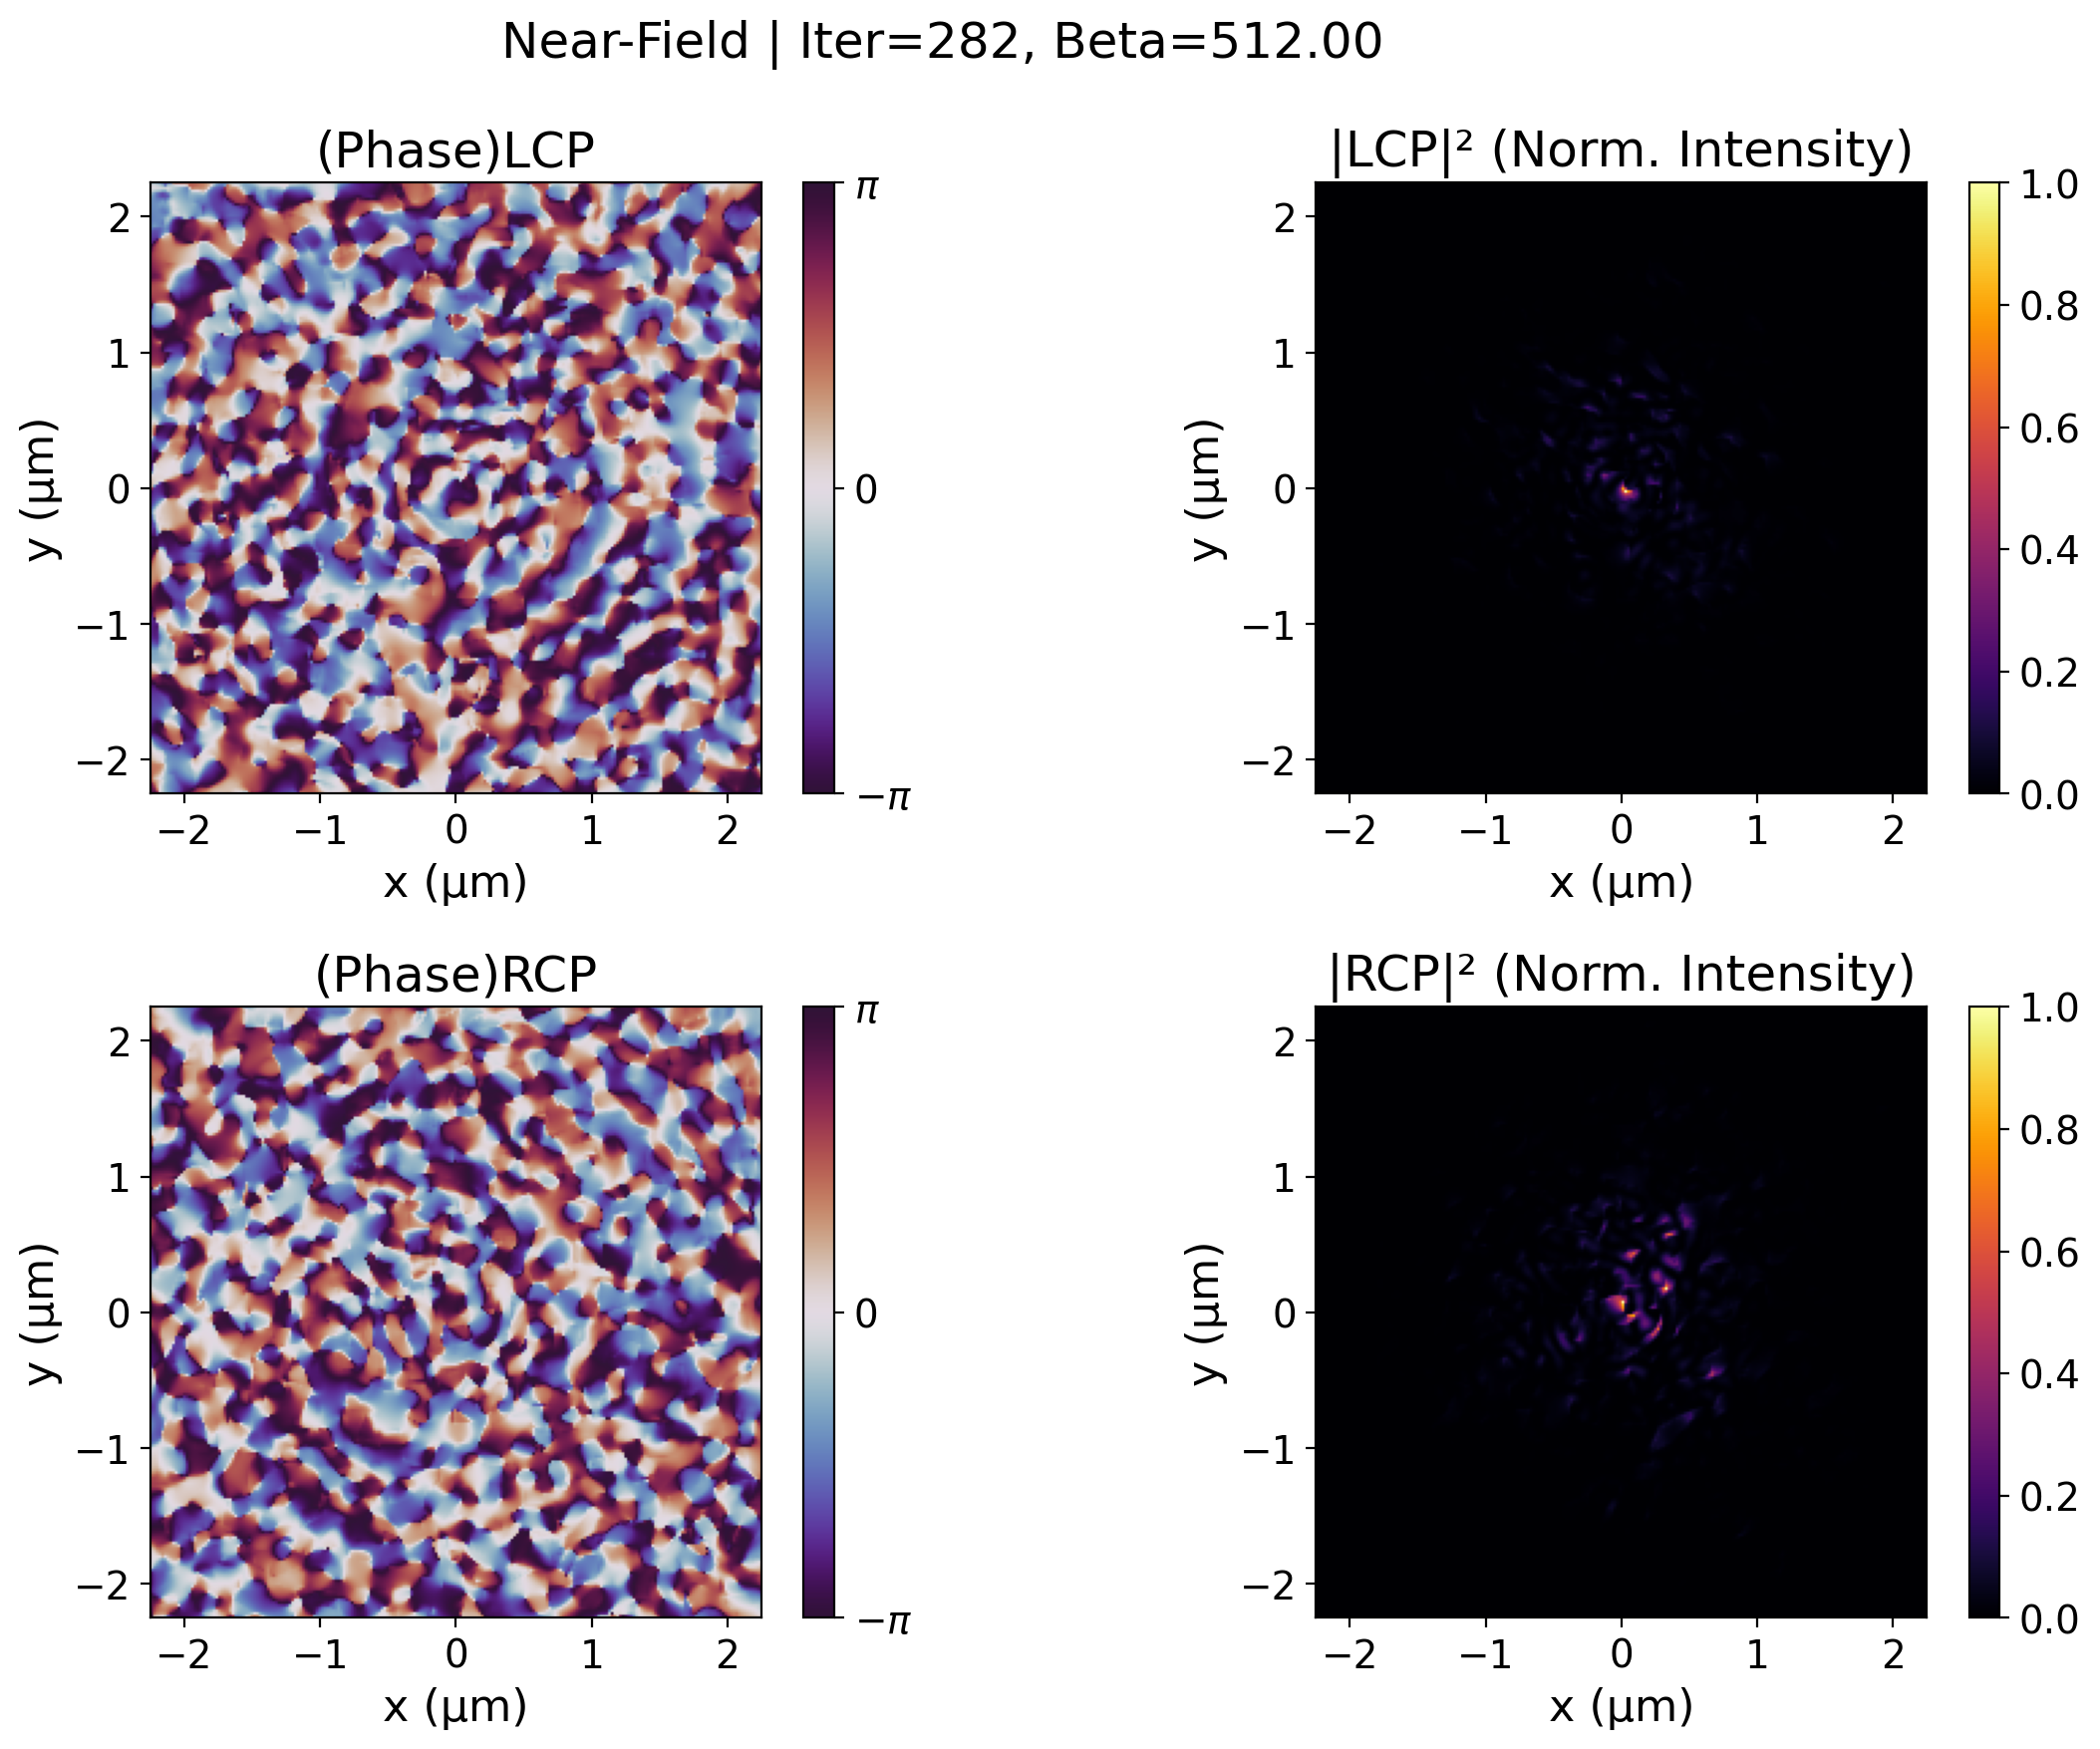
\includegraphics[width=0.47\textwidth]{img/020_phase_iter_282_beta_512.00.png}
	    \\  (c)  & (d) \\[6pt]
	    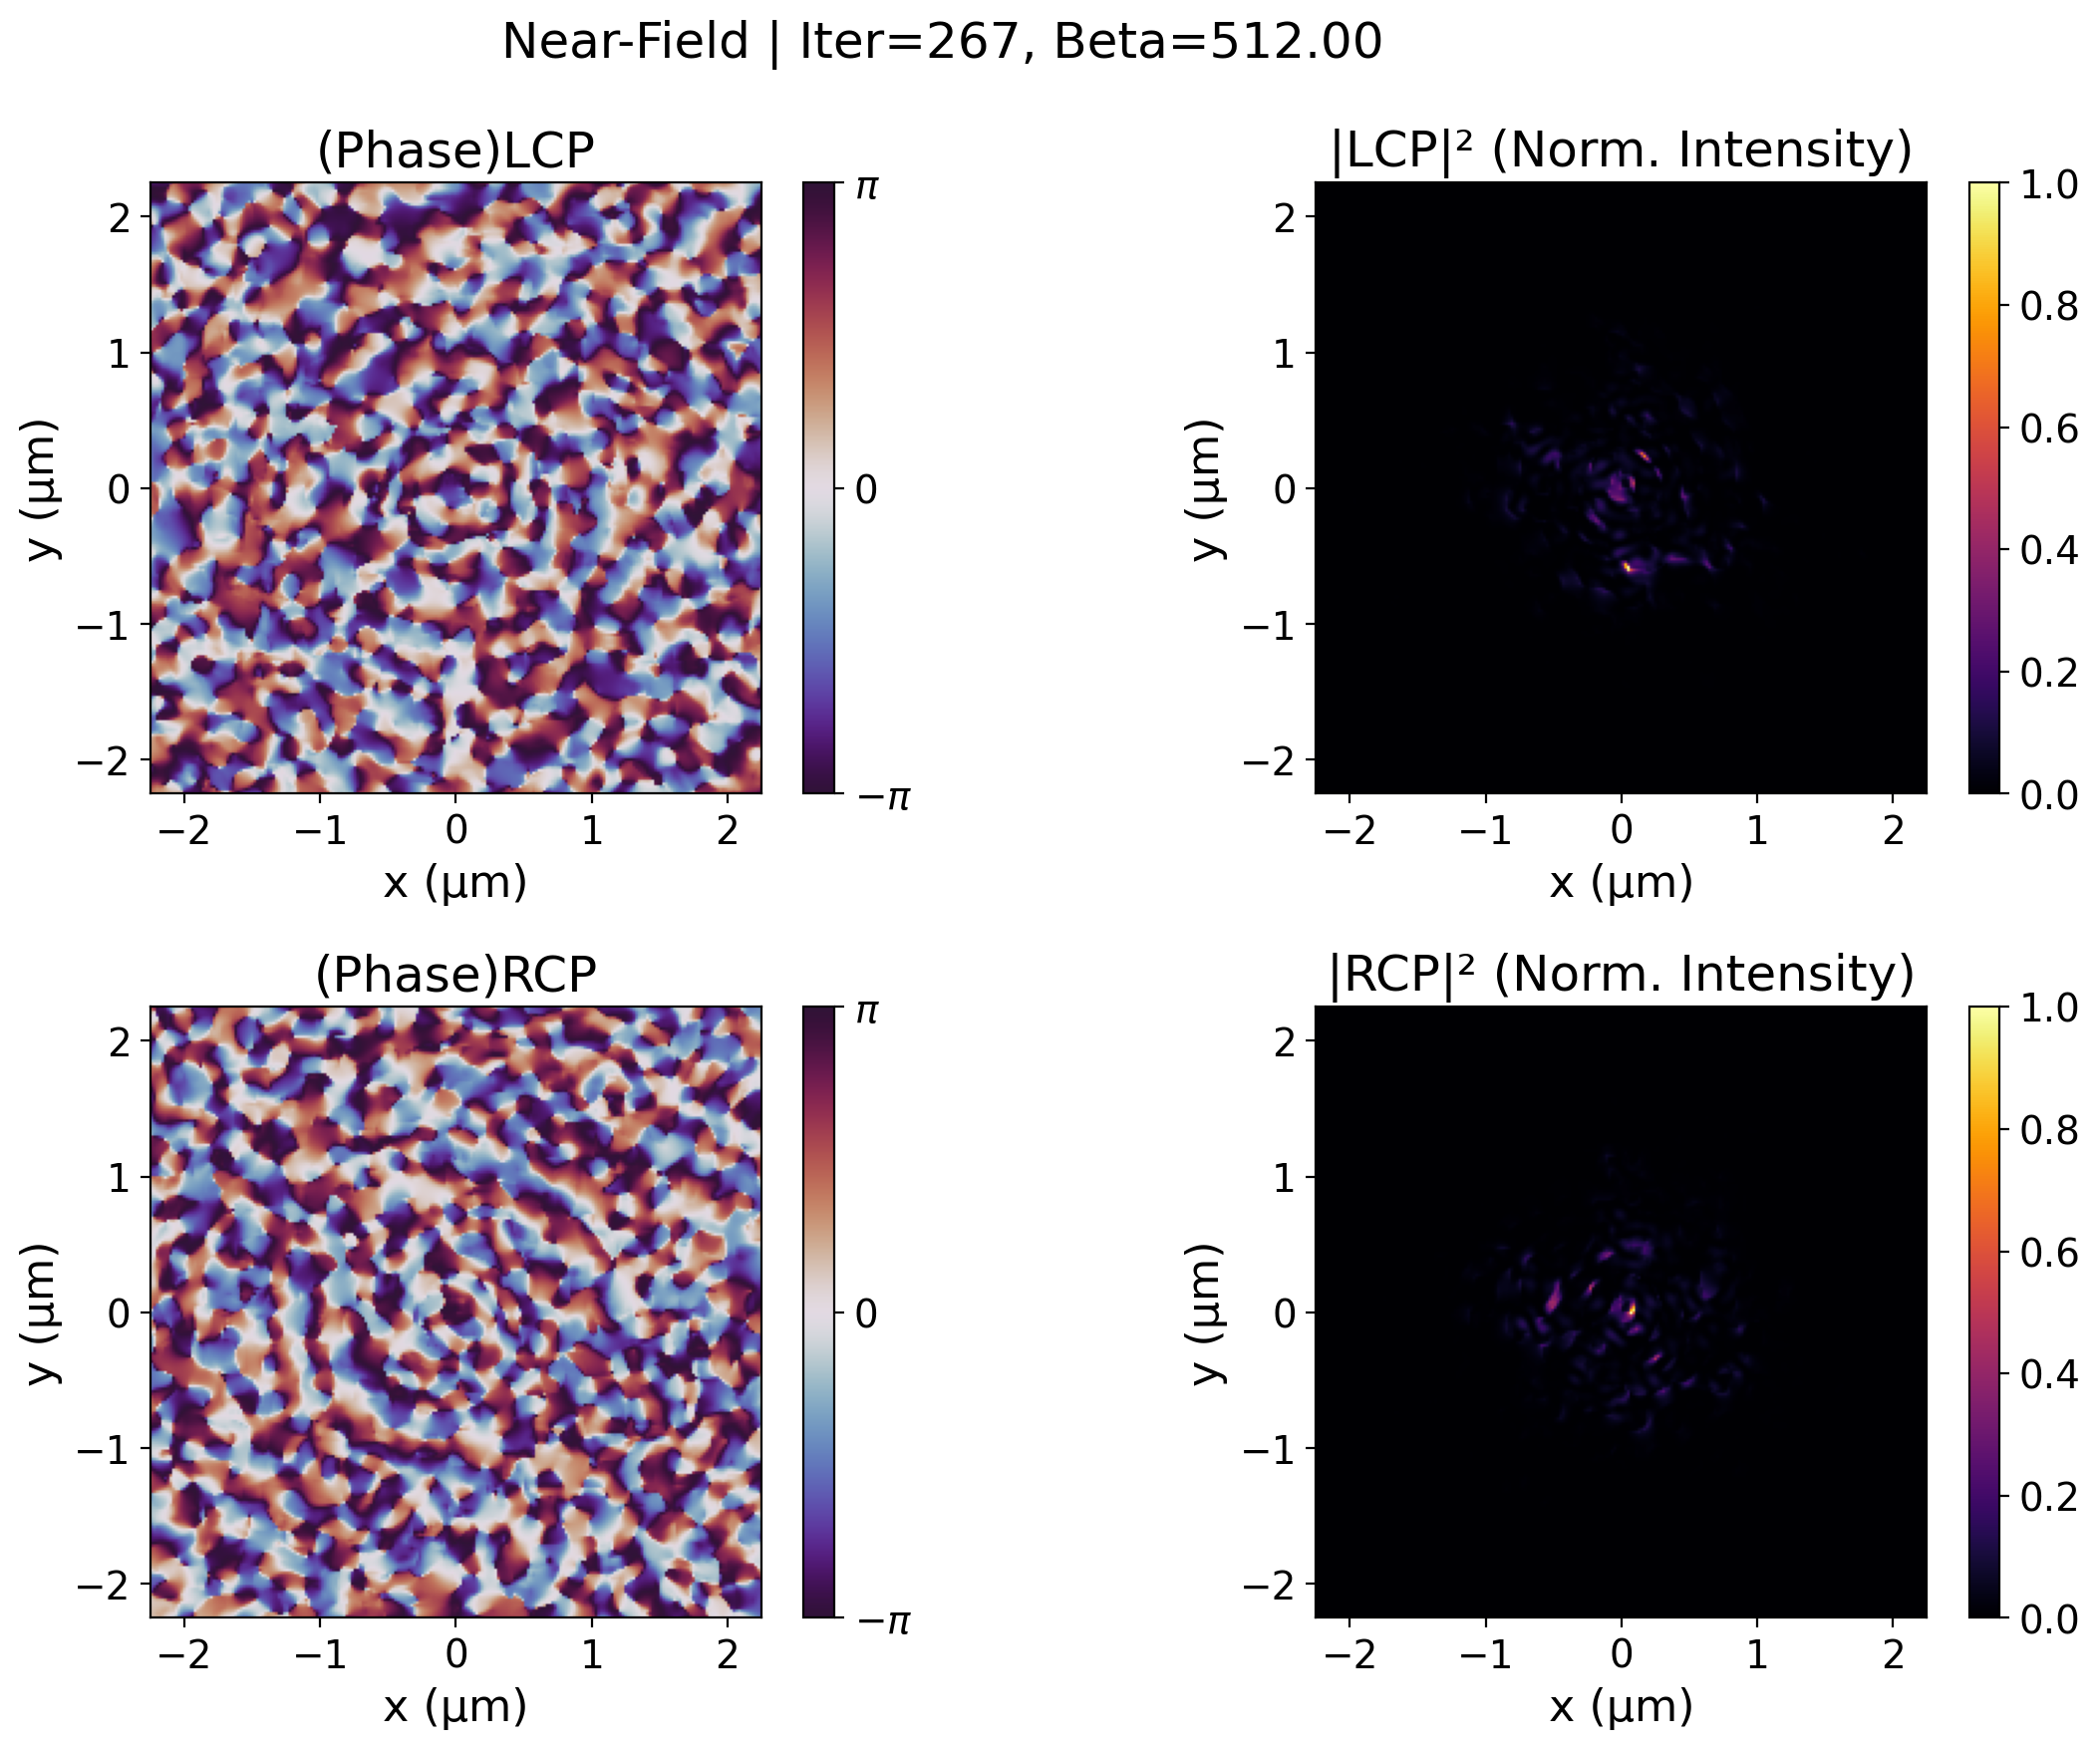
\includegraphics[width=0.47\textwidth]{img/021_phase_iter_267_beta_512.00.png}&
	    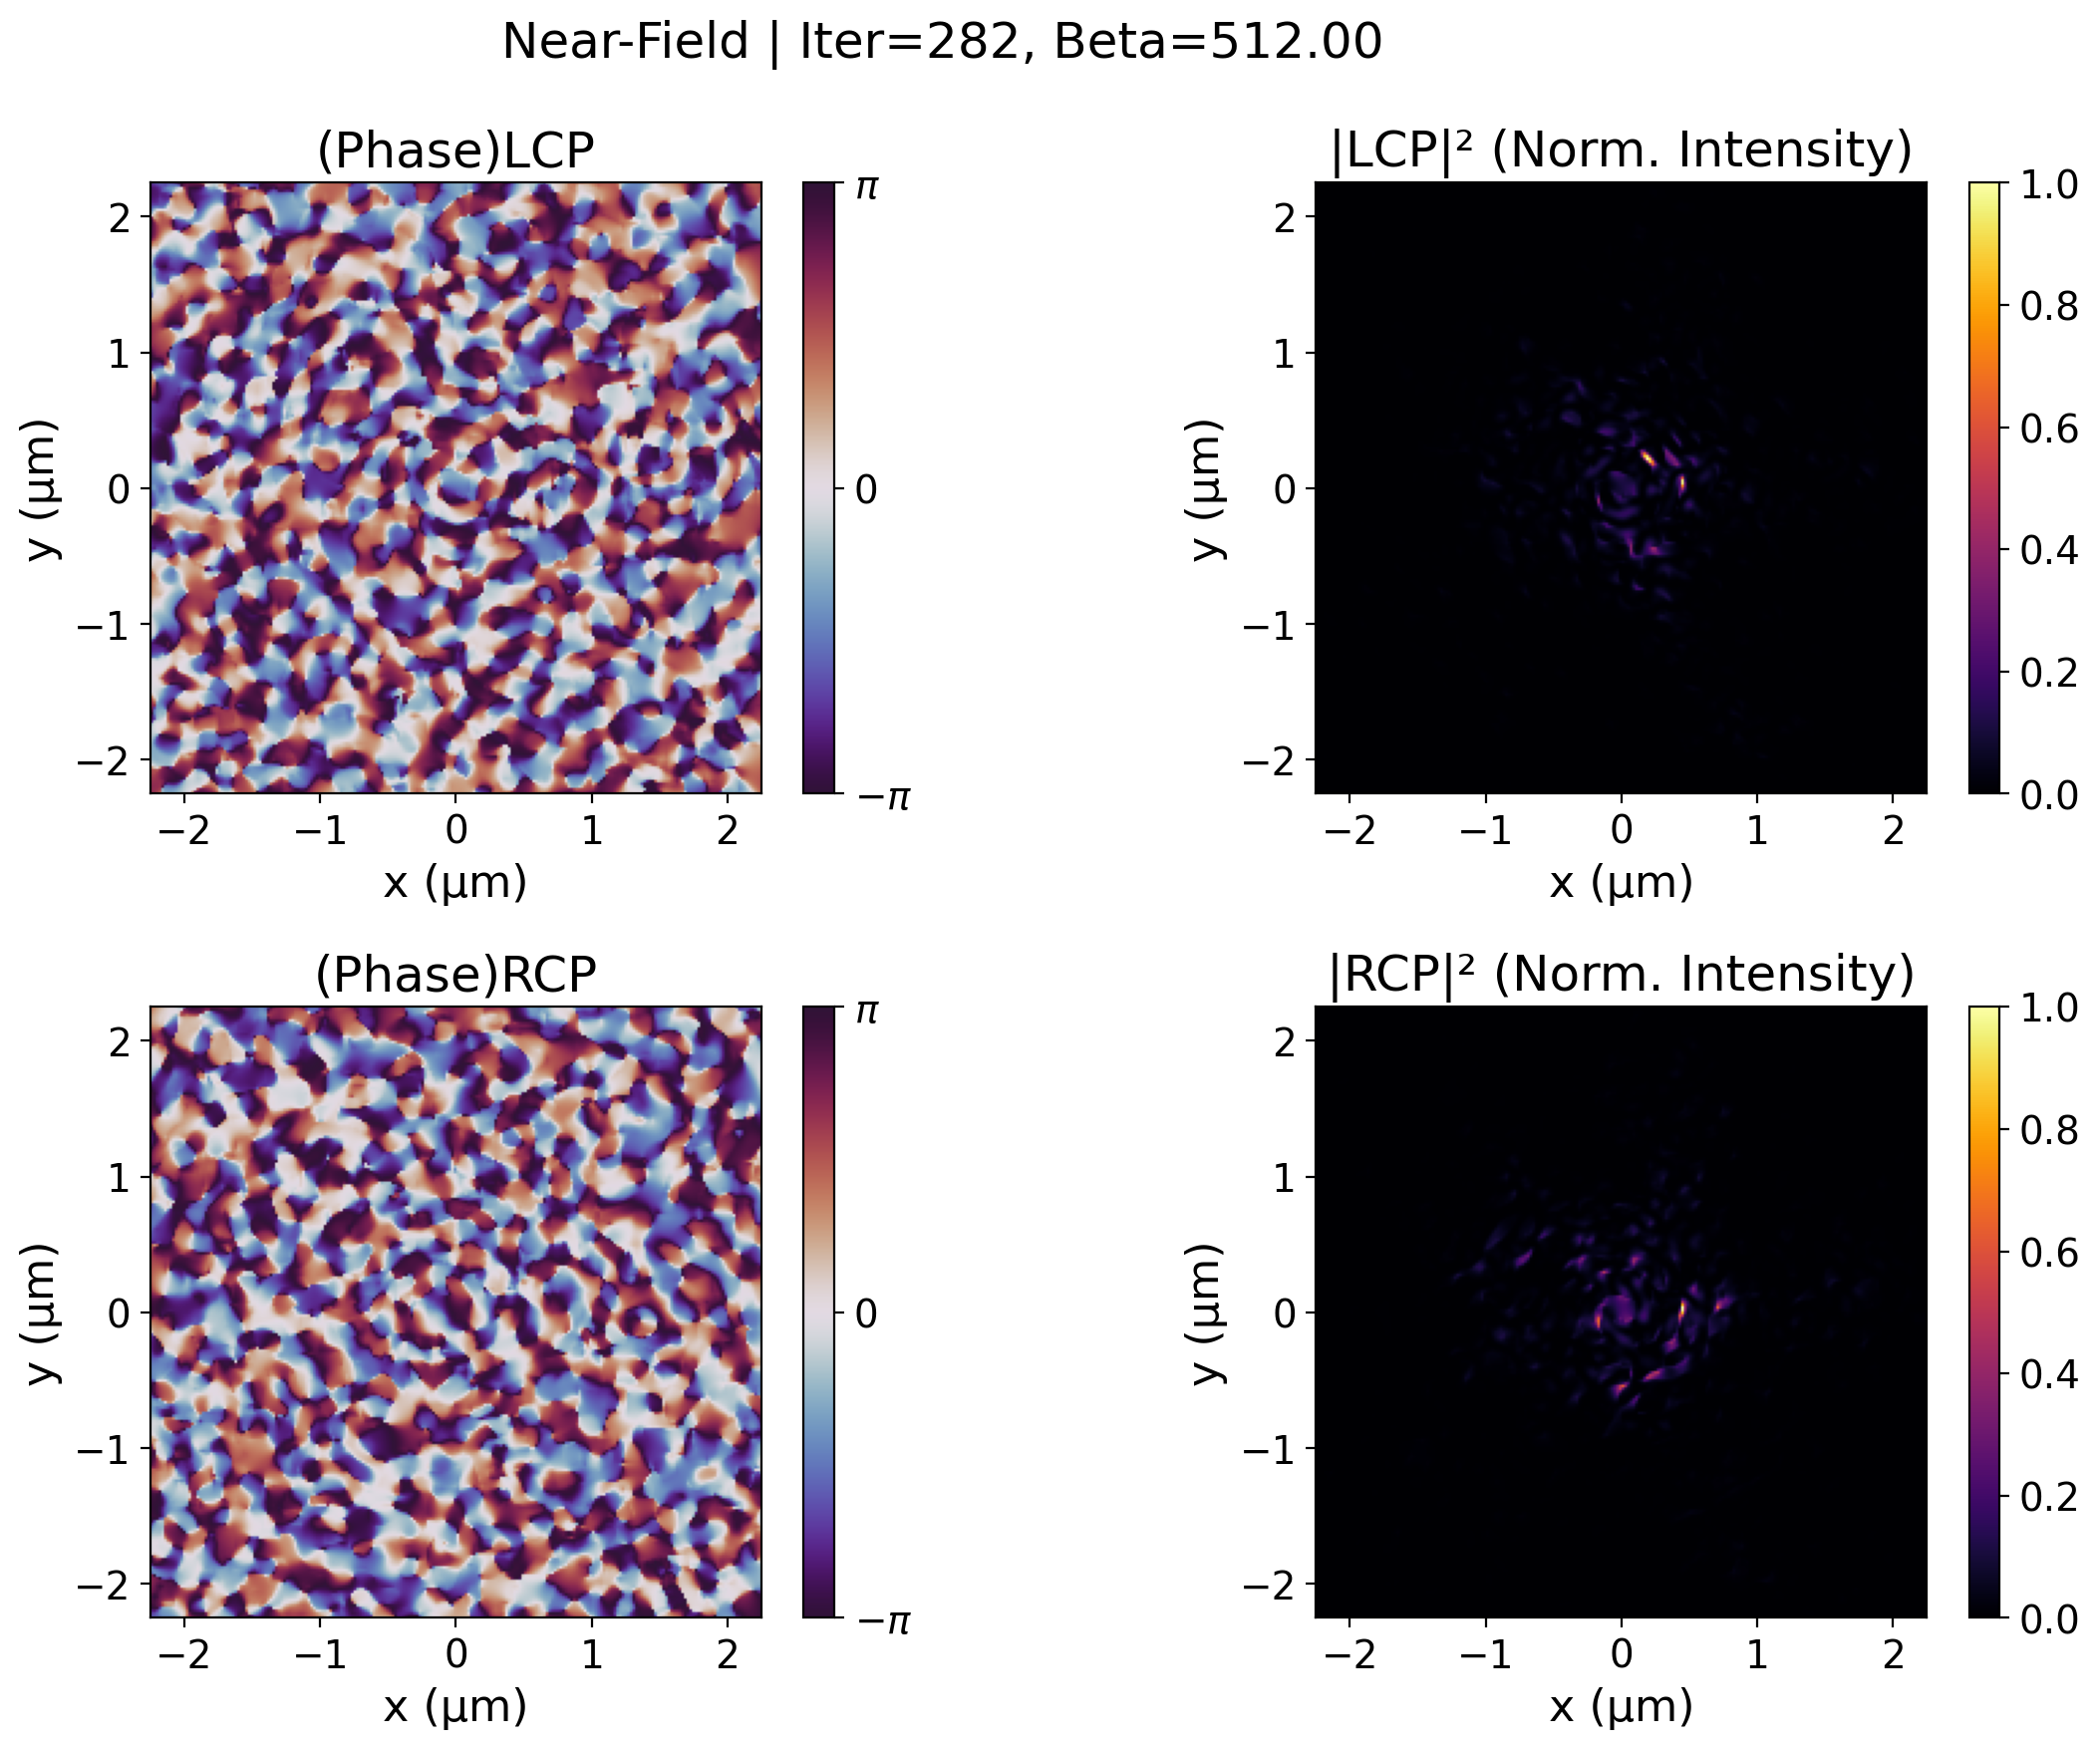
\includegraphics[width=0.47\textwidth]{img/022_phase_iter_282_beta_512.00.png}
	    \\ (e) & (f) 
	\end{tabular}
\caption{Near-field electric field distributions just above the design layer: (a)$\sim$(f) $\ell \in \{0, 1, 2, 3, 4, 5\}$, respectively. Each group of four panels: upper left — LCP phase; upper right — $|\text{LCP}|^2$ normalized intensity; lower left — RCP phase; lower right — $|\text{RCP}|^2$ normalized intensity.}
\label{fig:nearfield_all}
\end{figure}


%===================================================================

  
\section{Far-Field LG Mode Performance}

\label{sec:farfield}

Figure~\ref{fig:farfield_all} compares, in four-panel format, the simulated LCP phase and intensity (top row) and the theoretical phase and intensity of the target LG$_{\ell,0}$ mode (bottom row) for all six designs at the far-field evaluation plane $z = 10\,z_R$.

\textbf{Intensity distribution:} The $\ell = 0$ far field shows a Gaussian profile with a central intensity peak; all designs with $\ell \geq 1$ show a doughnut-shaped spot with zero center intensity, with the ring radius increasing with $\ell$, consistent with the LG mode theoretical prediction (peak radius $r_\text{peak} = w_0\sqrt{\ell/2}$). The ring spots for high topological charges $\ell = 4, 5$ are slightly uneven.

\textbf{Phase distribution:} The far-field phase for $\ell = 0$ to $2$ clearly shows the corresponding spiral structure. The number of spiral arms and their rotation direction match the target mode exactly, qualitatively confirming the correctness of the topological charge for each design (detailed quantitative verification in Section~\ref{sec:winding}). However, for high topological charges $\ell = 3$ to $5$, the spiral arms do not align as perfectly at the intensity center as in the low topological charge cases, and for $\ell = 4$ and $5$ the phase shows some irregularity. This deviation reflects the inherent difficulty of shaping high-order OAM modes within a finite design space.

\textbf{Quantitative results:} Purity and $|\text{Overlap}|^2$ for all six designs are listed in Table~\ref{tab:results_summary}. The overall trend shows that purity decreases as $\ell$ increases, remaining above $94\%$ for $\ell \leq 3$, and dropping to about $82\%$ for $\ell = 4, 5$. $|\text{Overlap}|^2$ drops significantly from $60.92$ at $\ell = 0$ to below $4.00$ for $\ell \geq 4$. Since the monitor area was dynamically adjusted based on the spot size for each topological charge to ensure a fixed coverage ratio, this sharp drop does not arise from geometric truncation. Notably, despite $\ell = 2$ achieving the highest LG modal purity among all non-Gaussian designs, its $|\text{Overlap}|^2$ value ($7.99$) is lower than that of $\ell = 3$ ($18.69$), revealing a non-monotonic dependence that is not governed solely by the finite design domain. The physical mechanisms behind both observations are discussed in Section~\ref{ssec:purity_overlap}.
\begin{figure}[htb]
\centering
	\begin{tabular}{cc} 
	    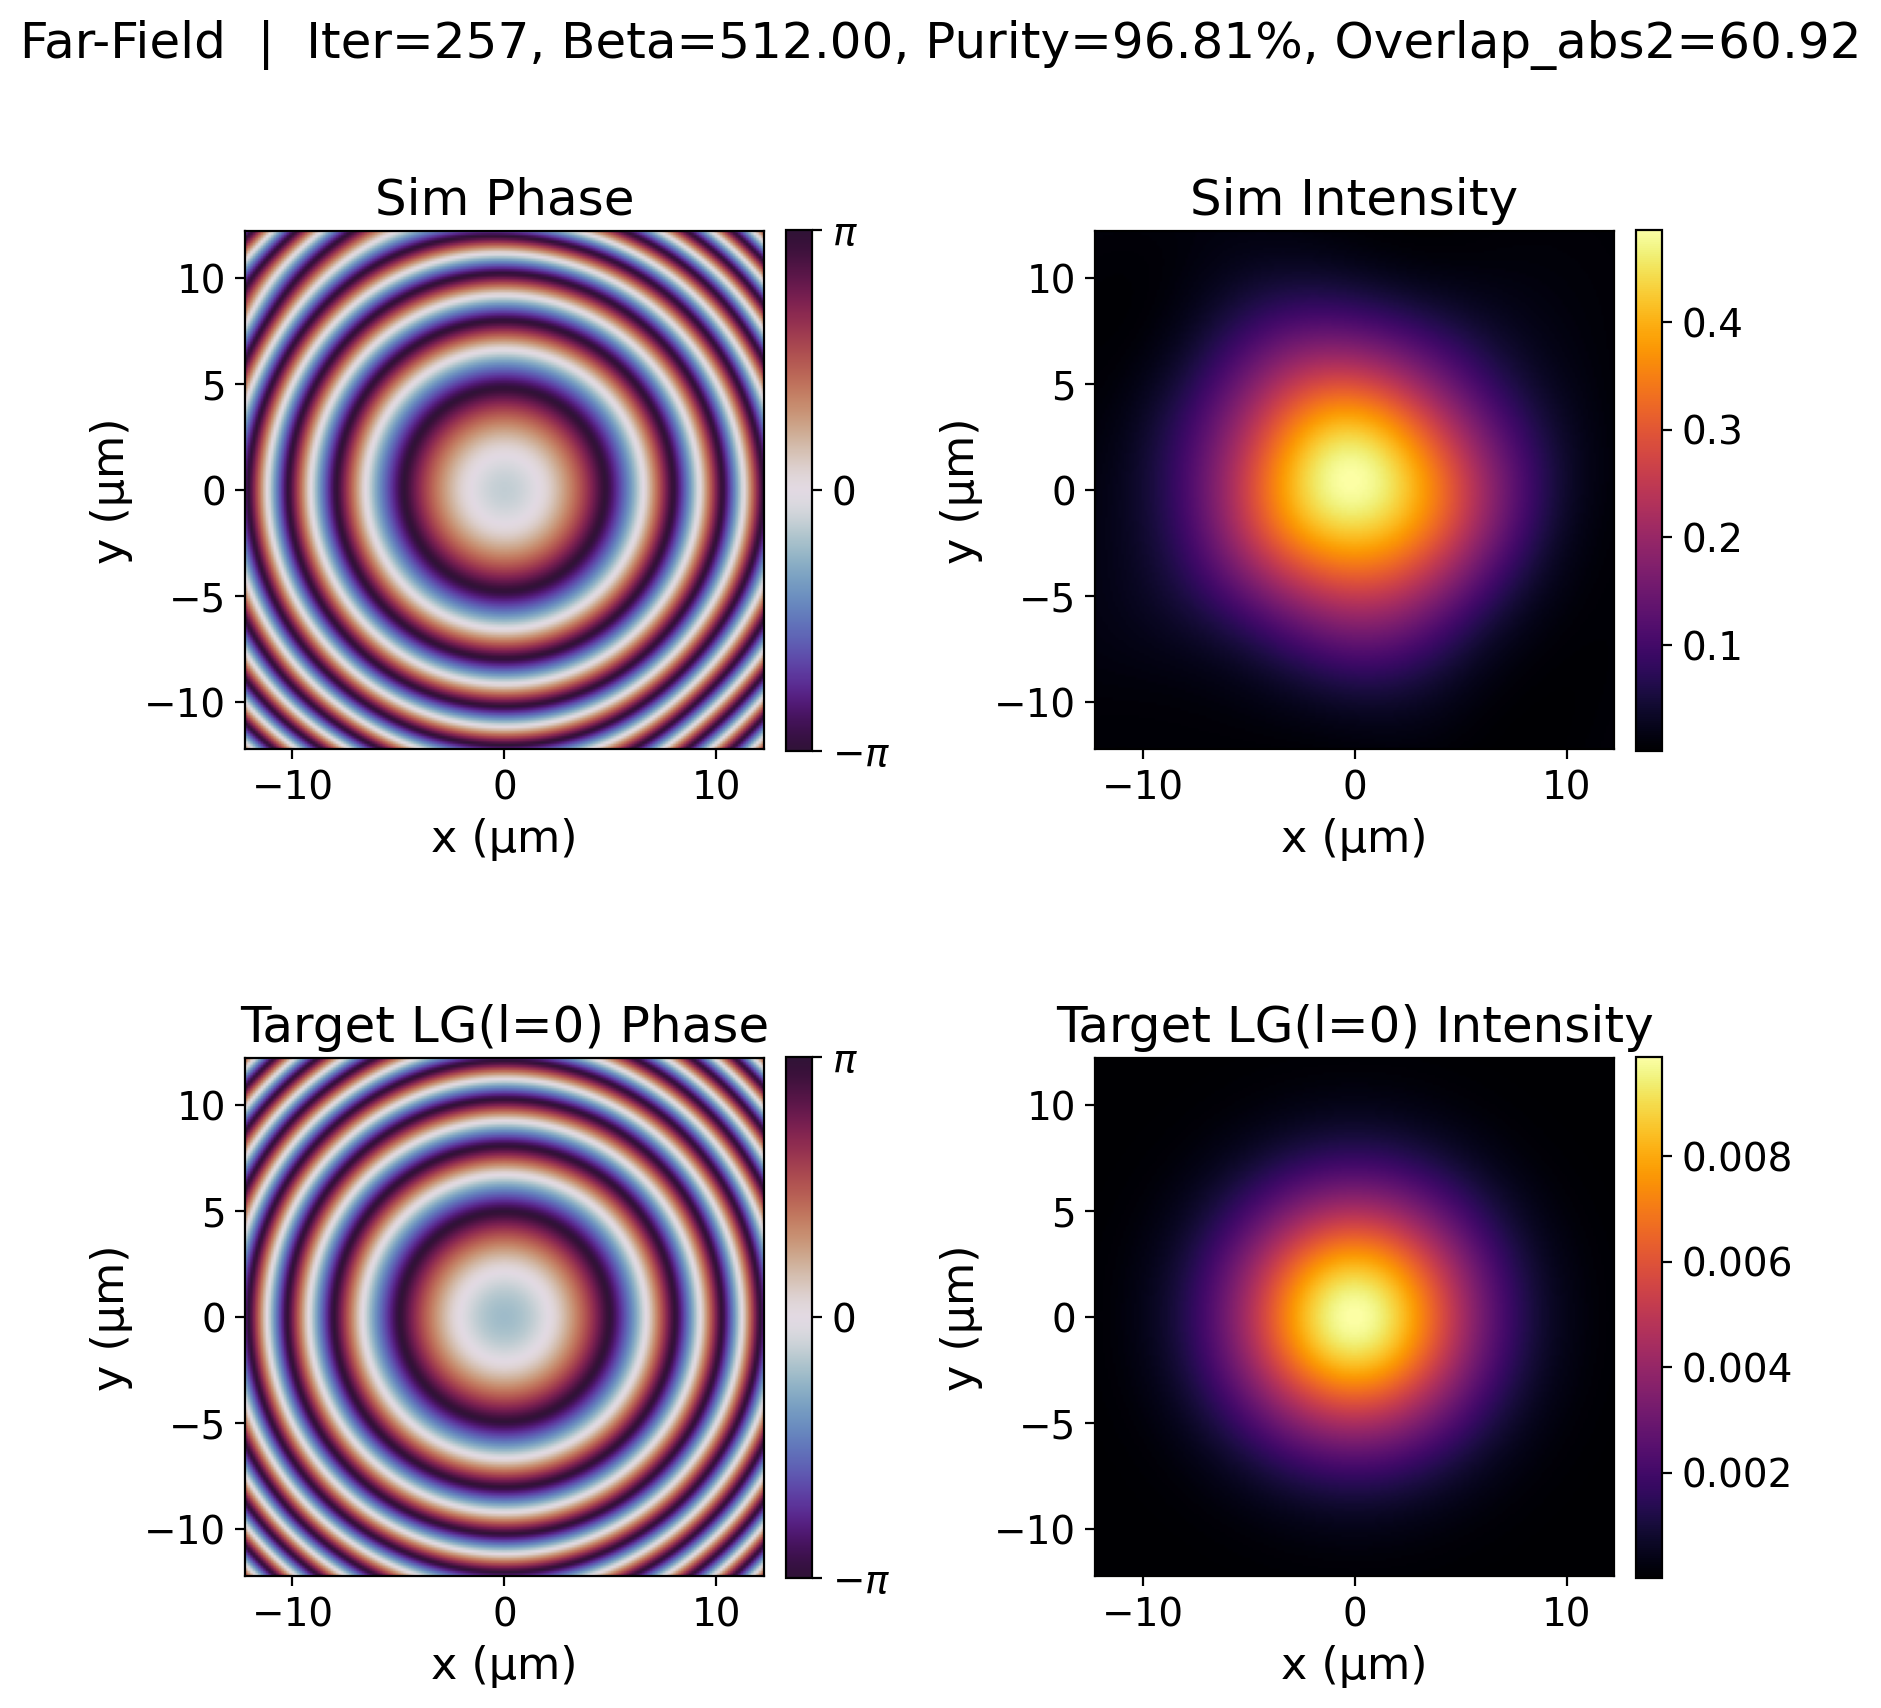
\includegraphics[width=0.47\textwidth]{img/017_ff_iter_257_beta_512.00.png}&
	    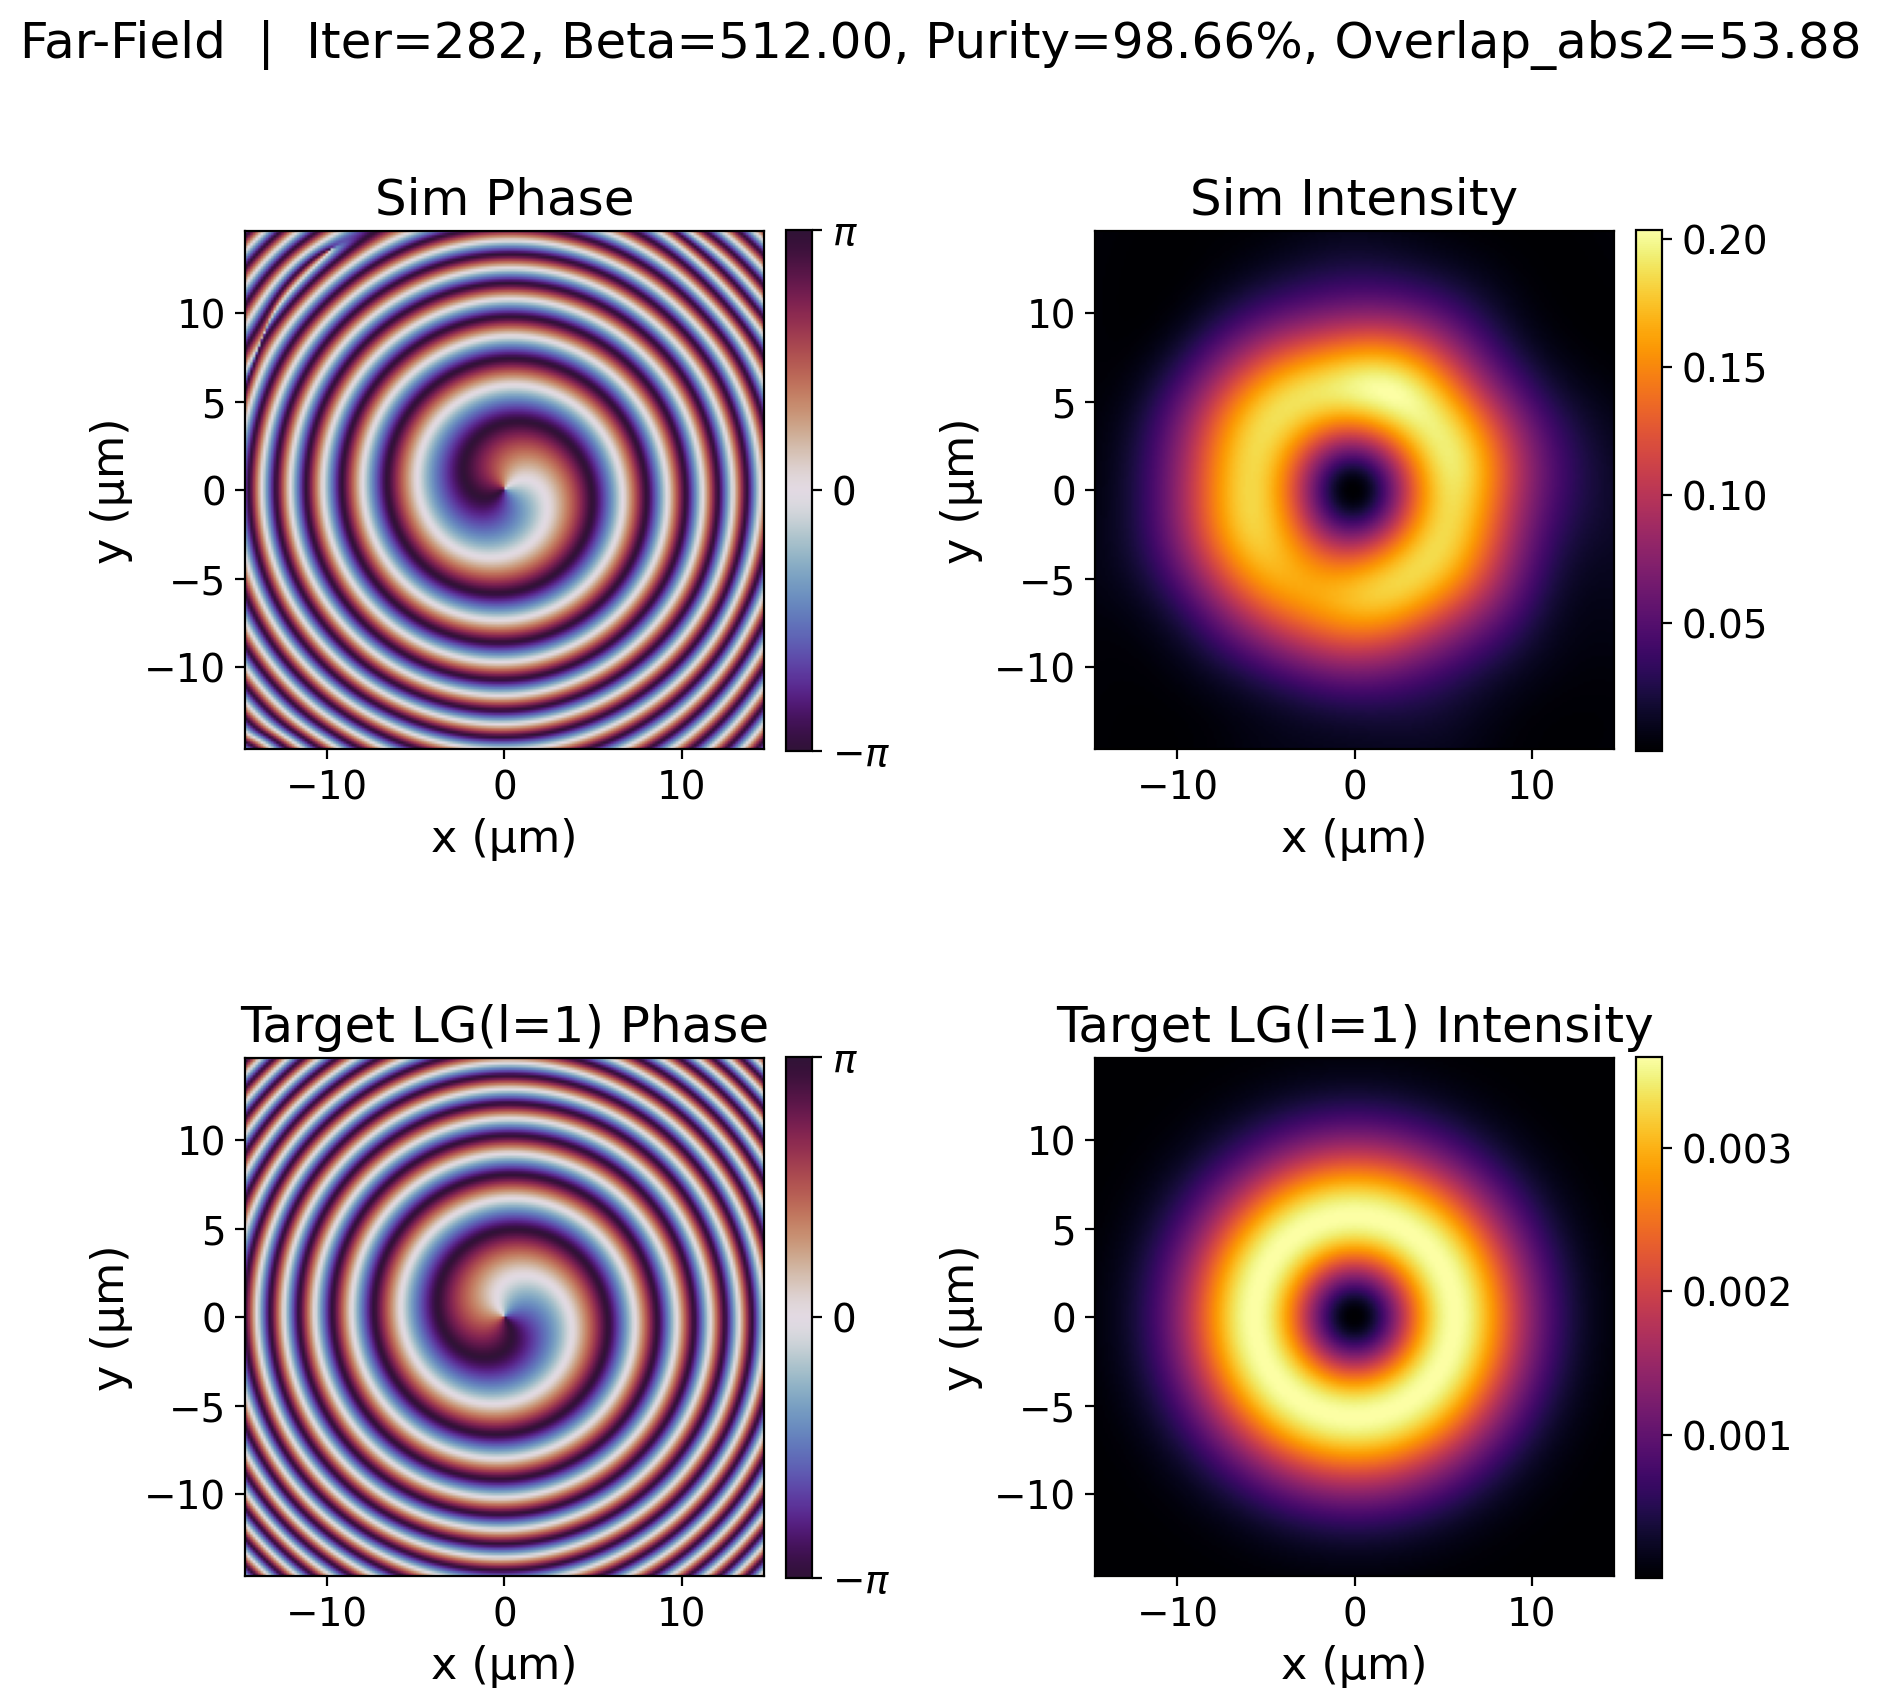
\includegraphics[width=0.47\textwidth]{img/018_ff_iter_282_beta_512.00.png}
		\\ (a) & (b)\\[6pt]
		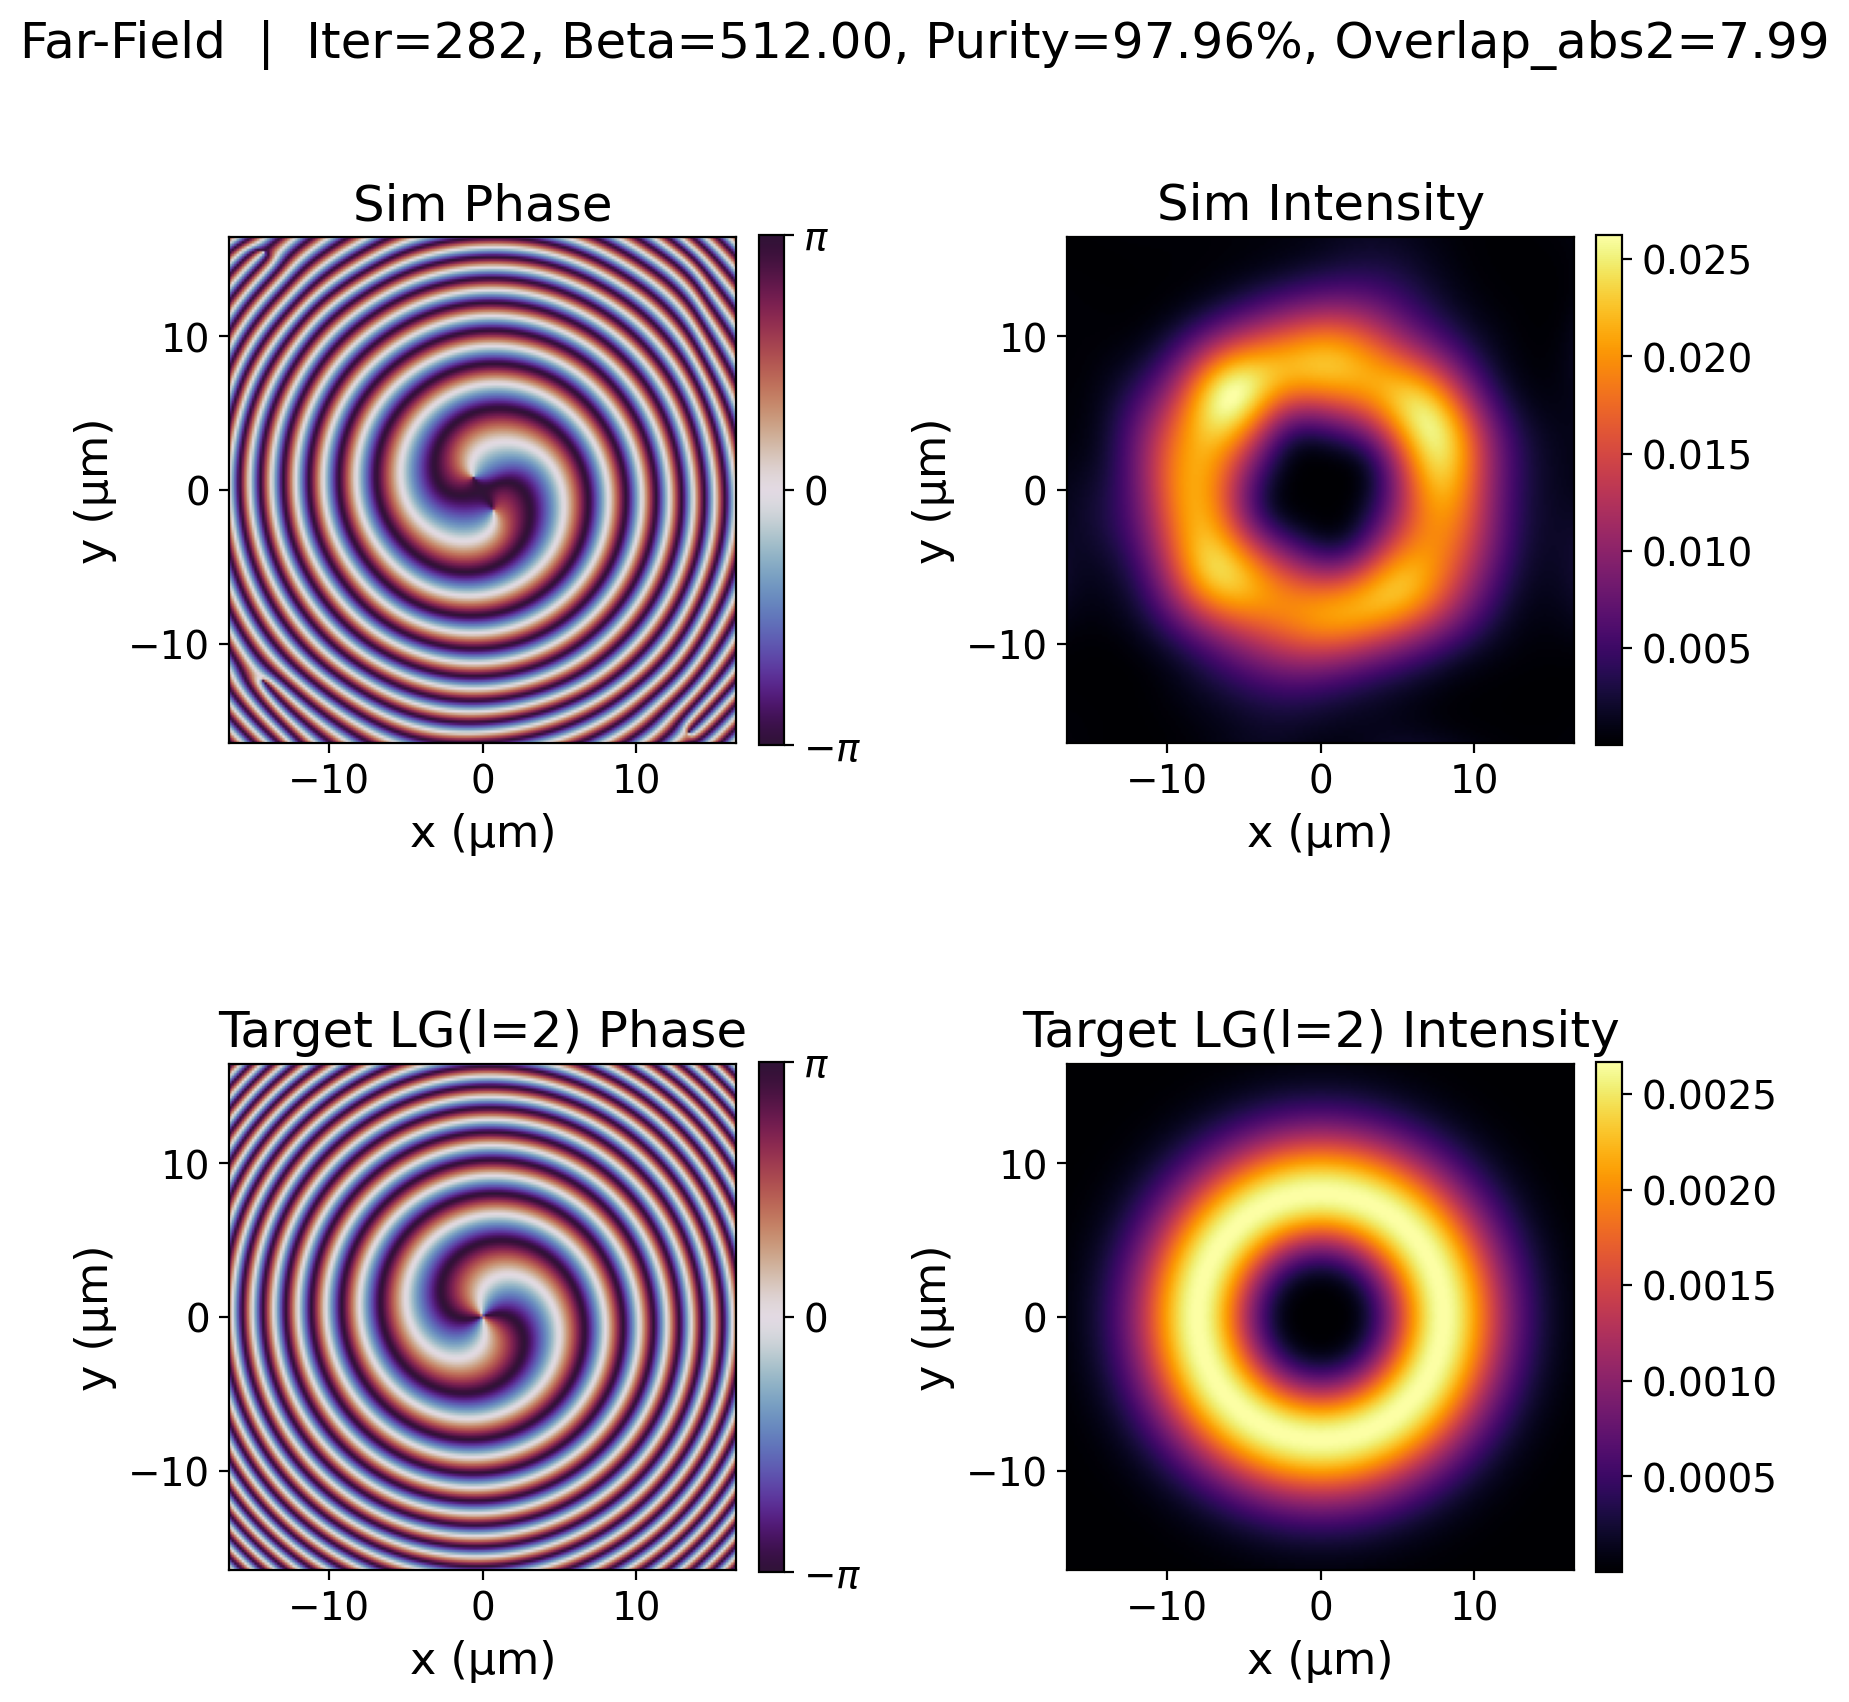
\includegraphics[width=0.47\textwidth]{img/013_ff_iter_282_beta_512.00.png}&
	    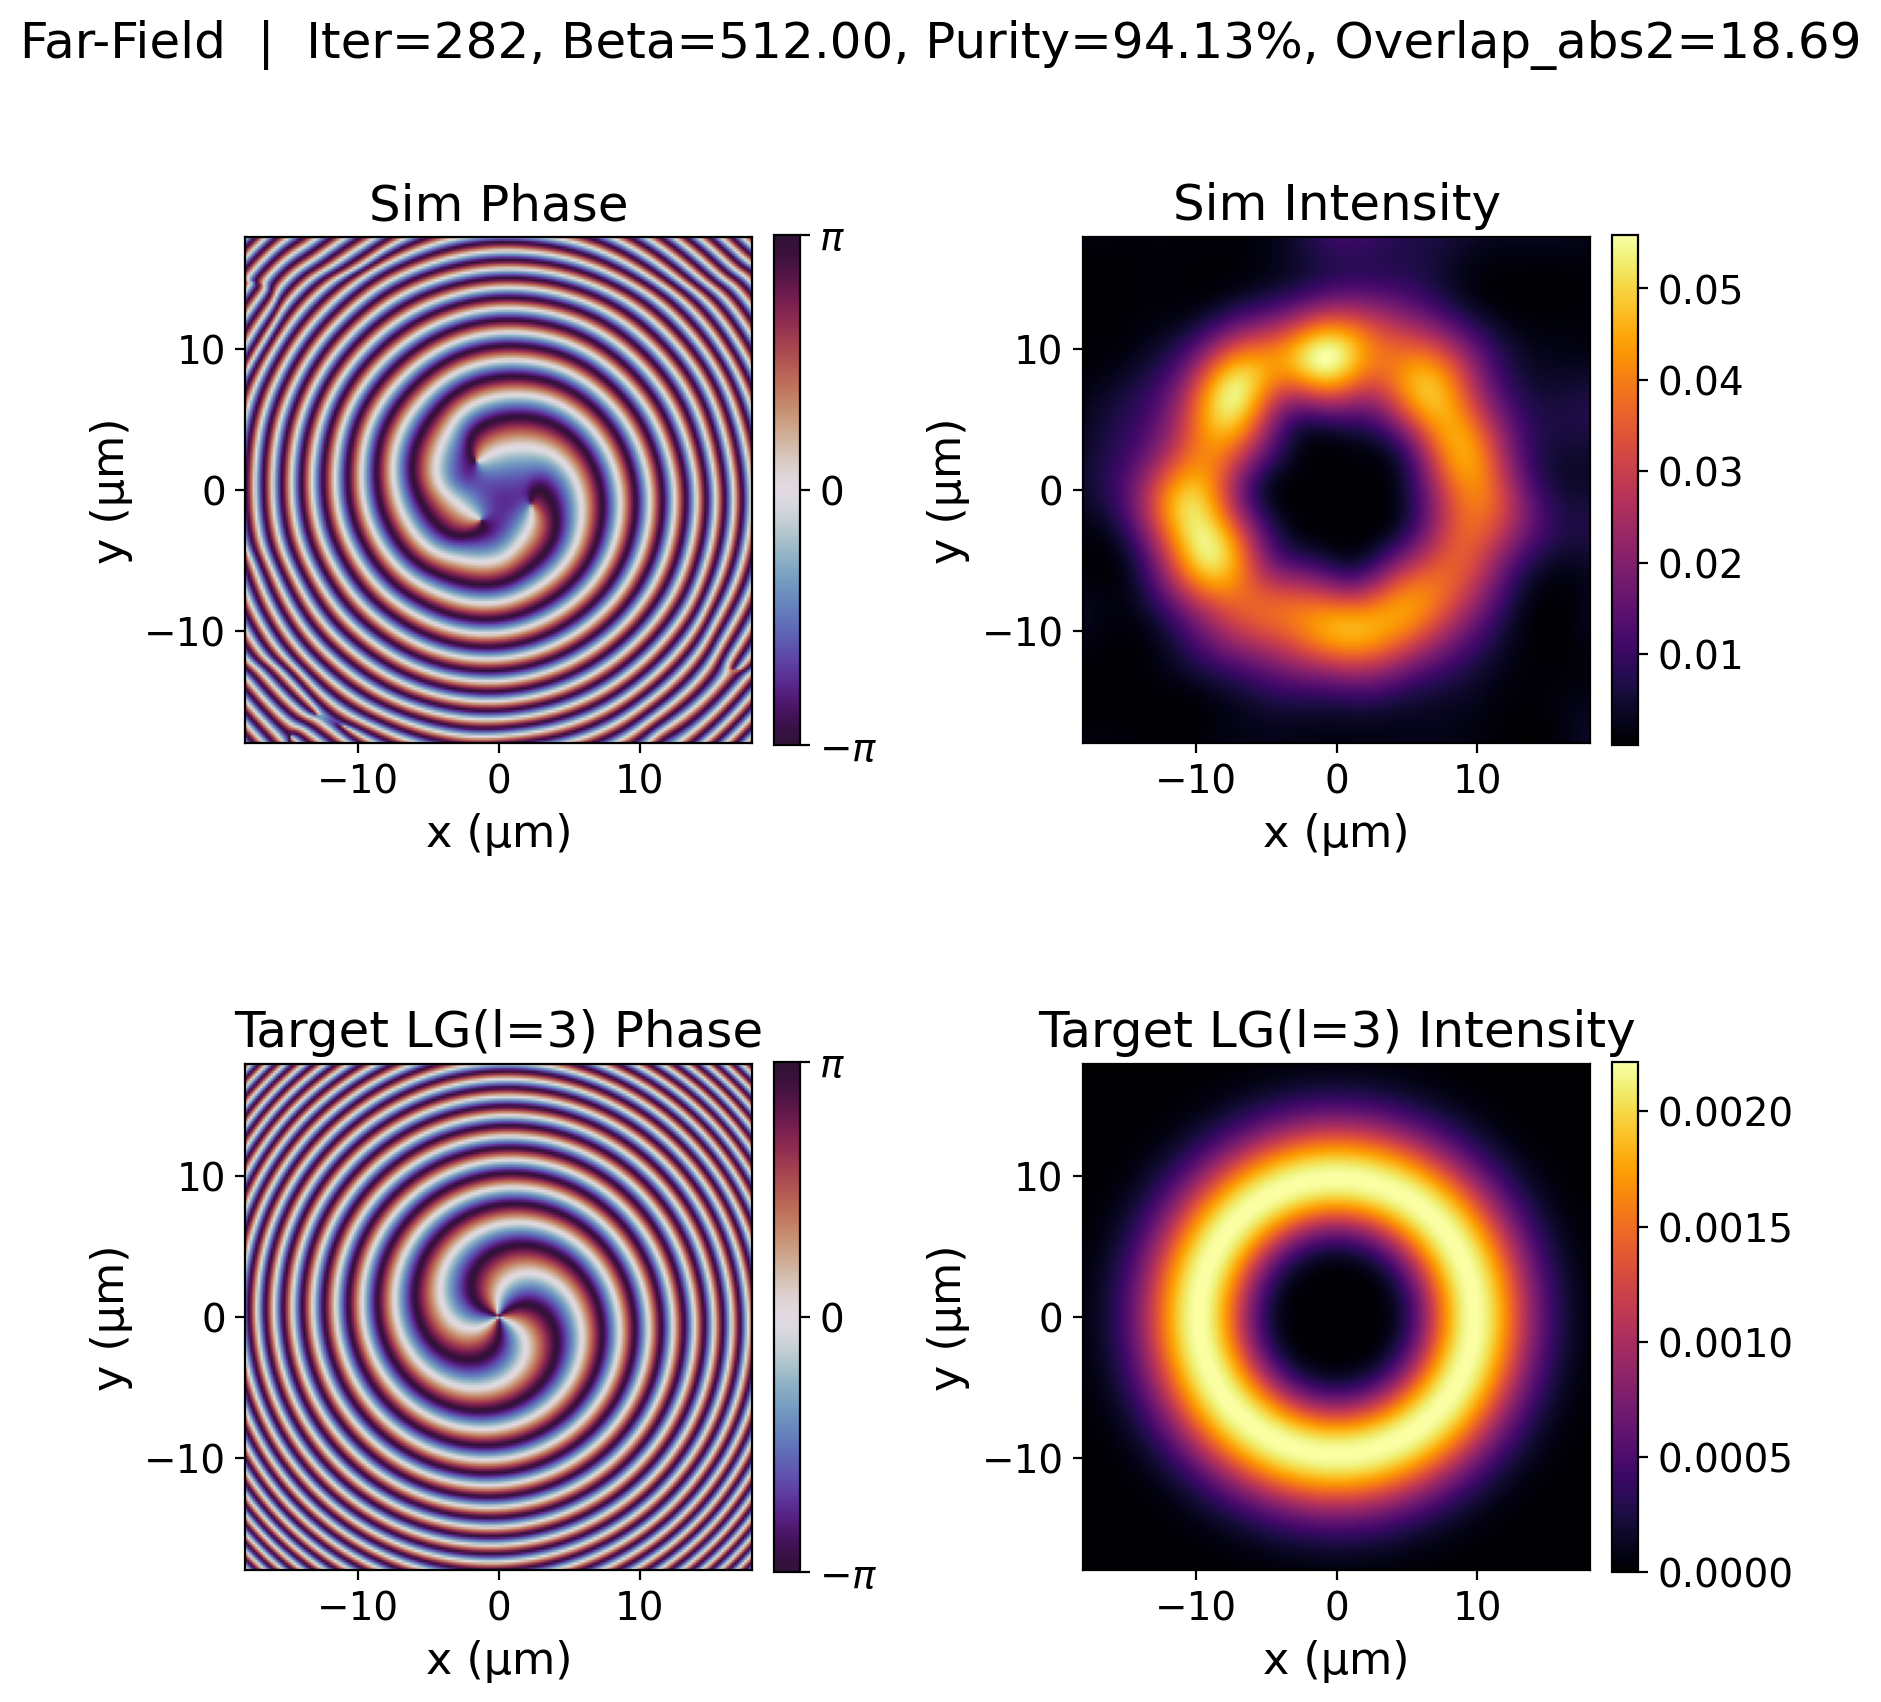
\includegraphics[width=0.47\textwidth]{img/020_ff_iter_282_beta_512.00.png}
	    \\(c) & (d)\\[6pt]
	    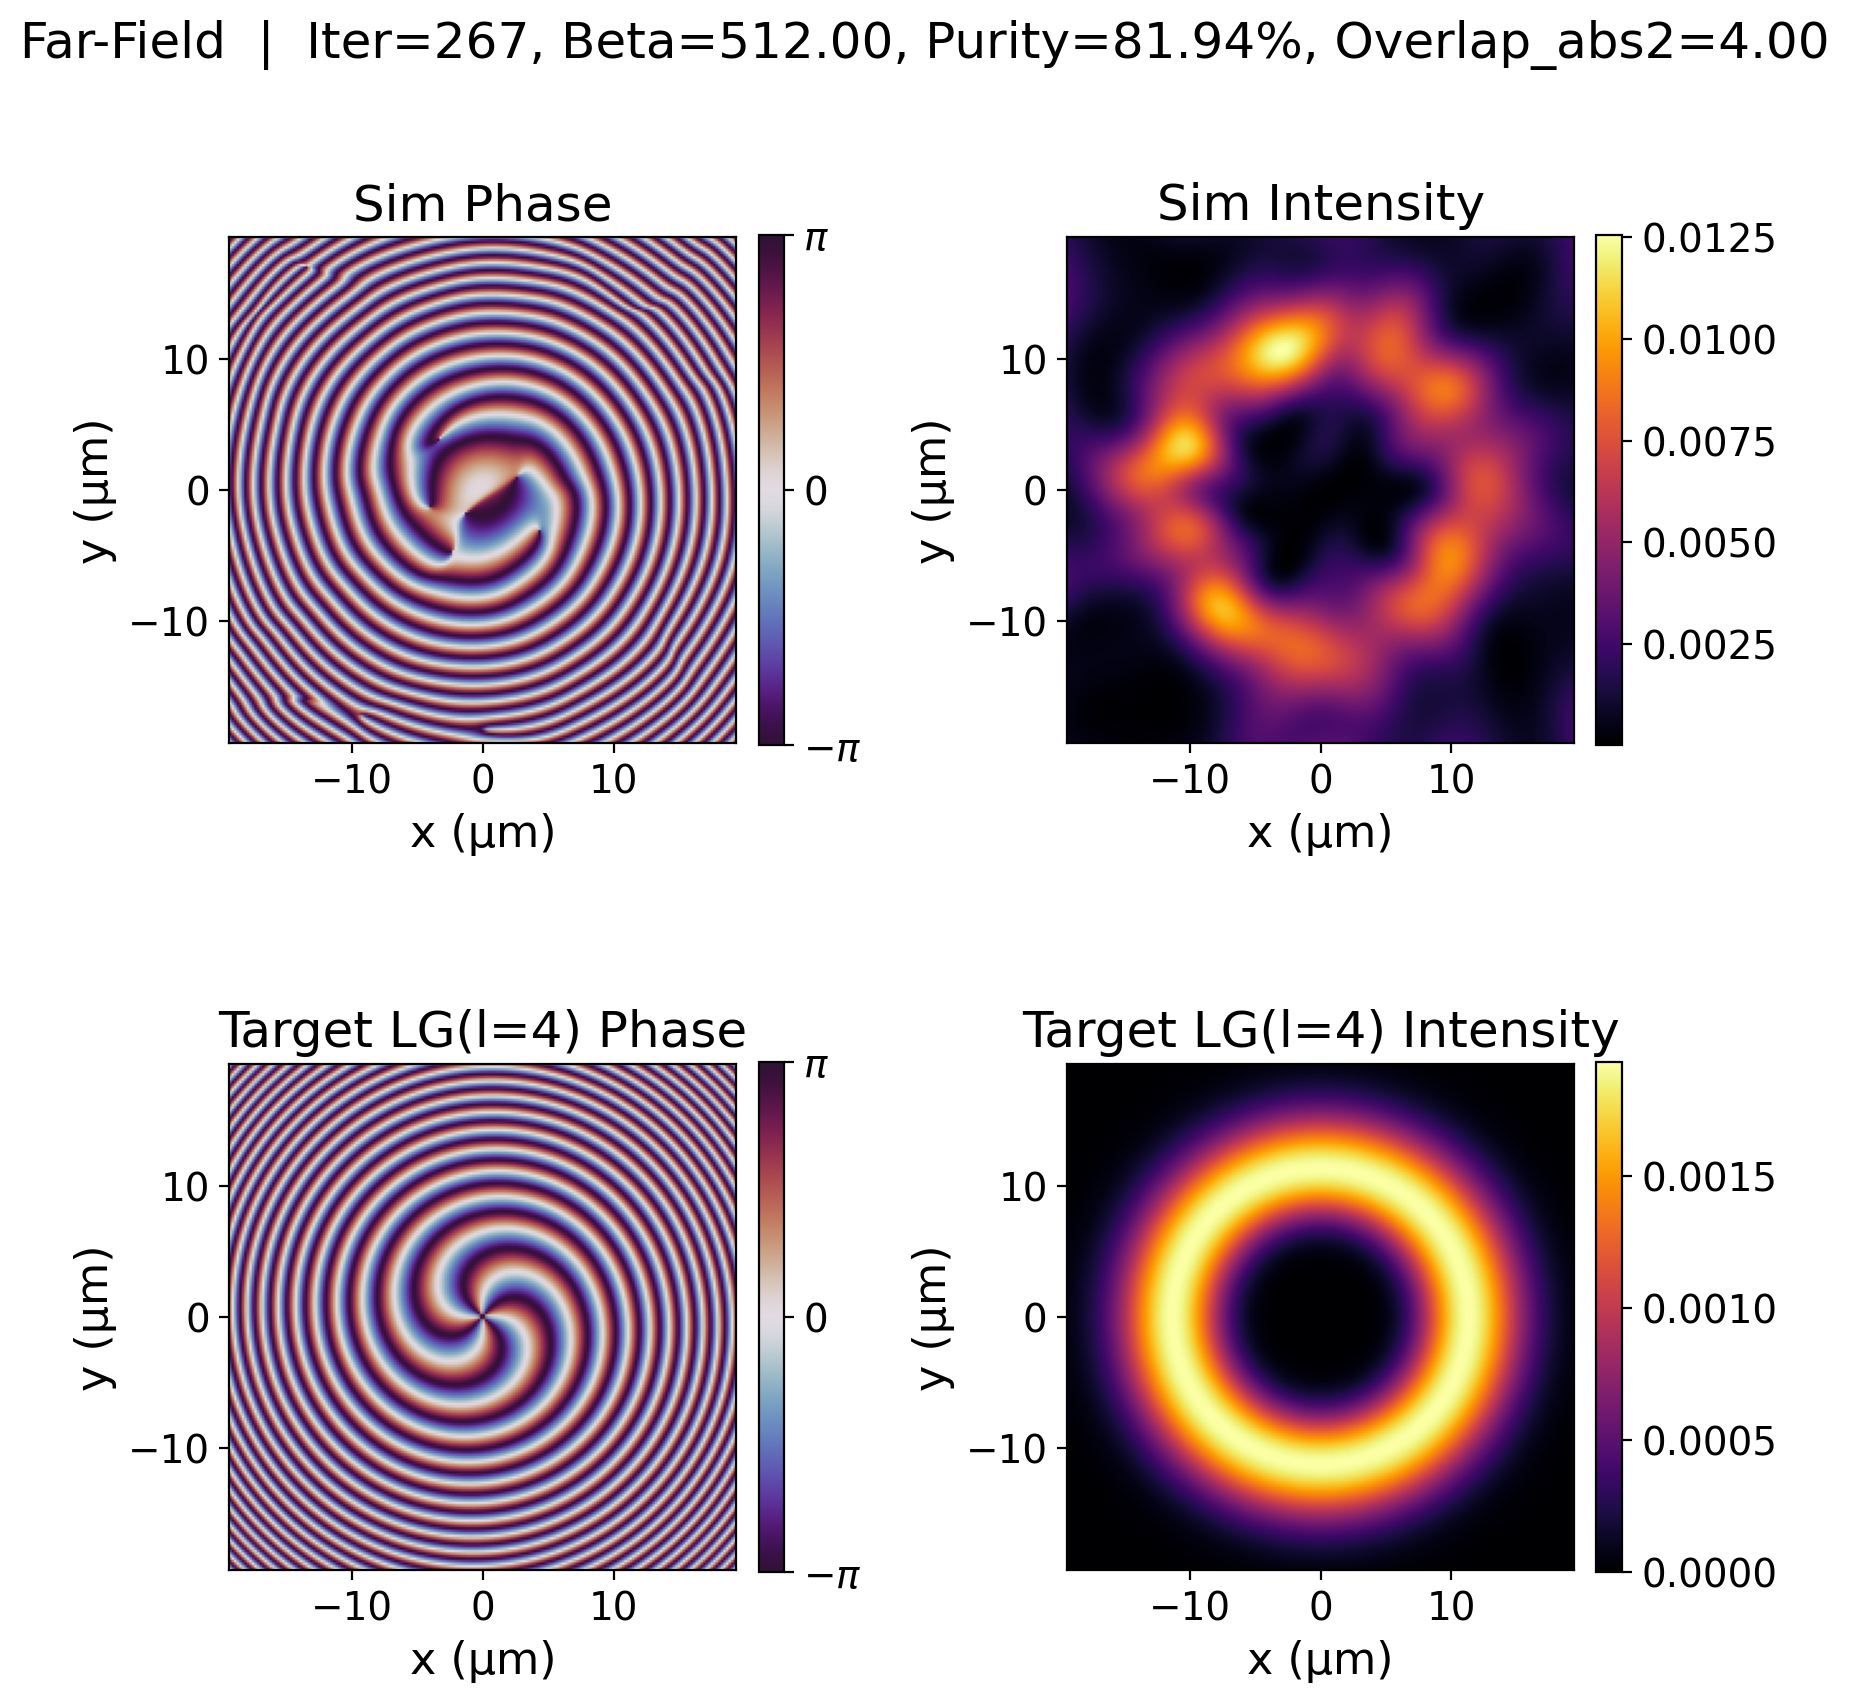
\includegraphics[width=0.47\textwidth]{img/021_ff_iter_267_beta_512.00.png}&
	    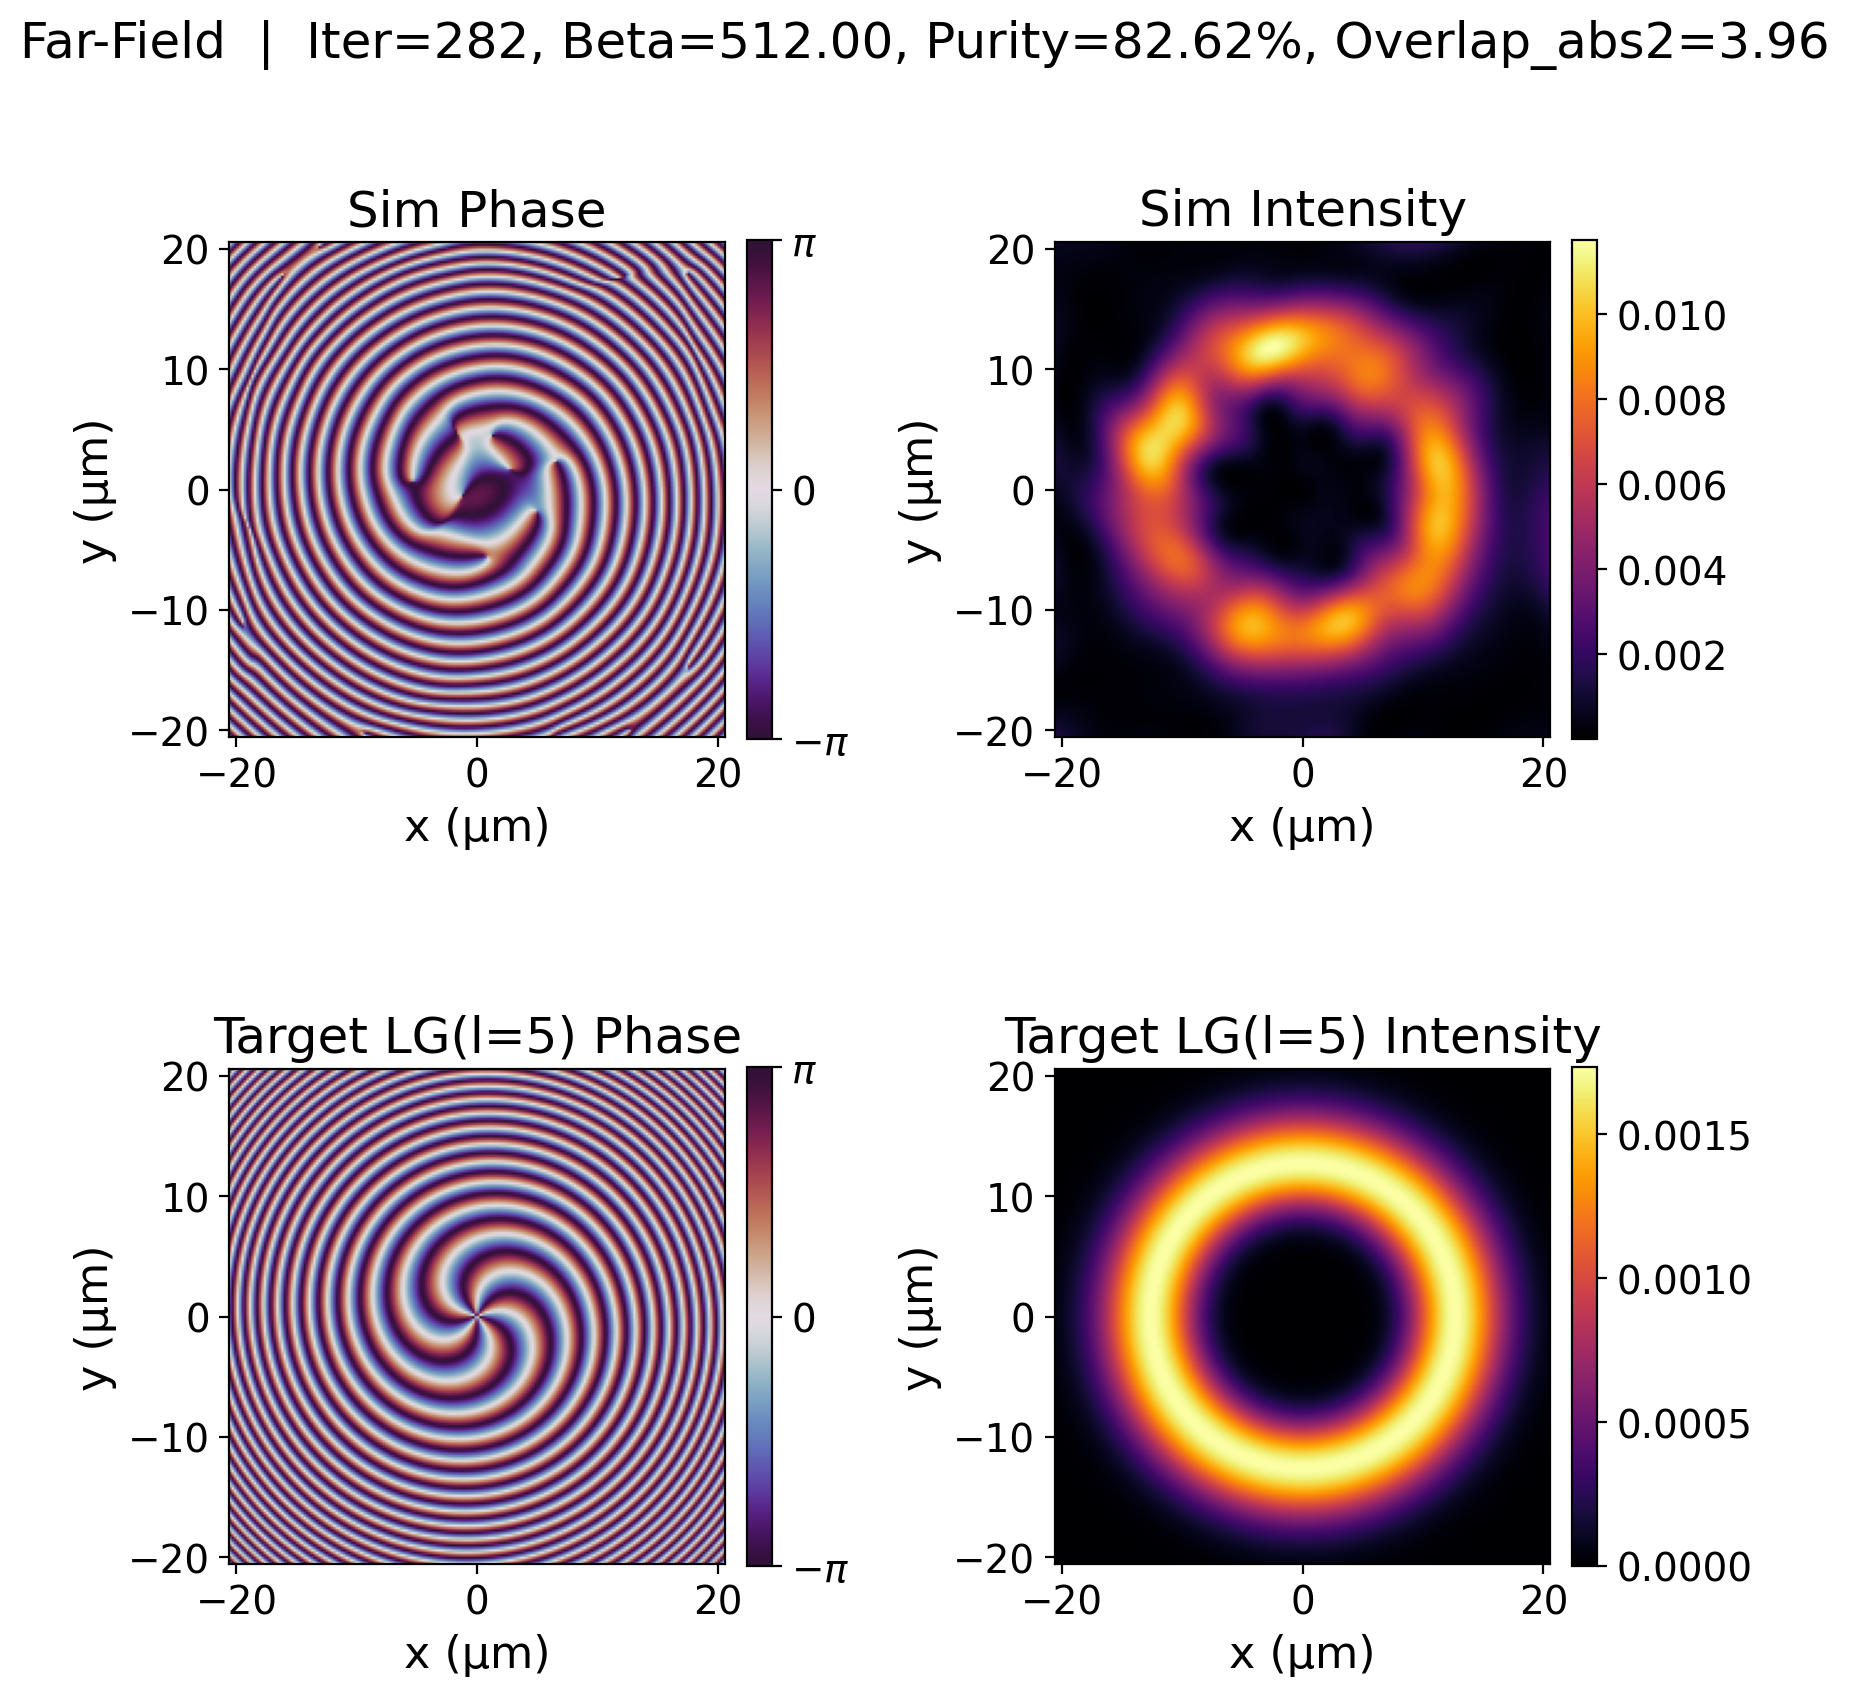
\includegraphics[width=0.47\textwidth]{img/022_ff_iter_282_beta_512.00.png}
	    \\(e) & (f)
	\end{tabular}
\caption{Far-field LG mode analysis ($z = 10\,z_R$): (a)$\sim$(f) $\ell \in \{0, 1, 2, 3, 4, 5\}$, respectively. Each group of four panels: upper left — simulated LG$_{\ell,0}$ phase; upper right — simulated LG$_{\ell,0}$ intensity; lower left — target LG$_{\ell,0}$ phase; lower right — target LG$_{\ell,0}$ intensity. Purity and $|\text{Overlap}|^2$ values are indicated at the top of each group.}
\label{fig:farfield_all}
\end{figure}

%===================================================================


\section{Optical Chirality}
\label{sec:chirality}

The optical chirality density $C \propto -\omega\,\varepsilon_0\,\text{Im} (\mathbf{E}^* \cdot \mathbf{B})$ quantifies the chiral character of the electromagnetic field in space: $C > 0$ indicates RCP dominance; $C < 0$ indicates LCP dominance. This section first uses the high-order mode ($\ell = 5$) as a representative case to analyze how optical chirality evolves along the propagation axis ($z$-axis), and then compares the near-field and far-field chirality distributions across all six designs.

\subsection{Chirality Propagation}
\label{ssec:chirality_prop}
To clarify the physical mechanism of chirality evolution during beam propagation, Figure~\ref{fig:chirality_prop} shows cross-sections of the optical chirality density distribution for the $\ell = 5$ mode propagating from the near field ($z \approx 0^+$) to the far field ($z = 10\,z_R$).

The results show that the near-field region ($z \ll z_R$) displays a pronounced LCP/RCP mixed state, strongly influenced by the intense local scattering and evanescent wave coupling of the topological structure; a substantial fraction of the area above the point source shows blue positive values ($C > 0$), indicating local RCP-dominant components generated by near-field scattering from the nanostructure. However, as the propagation distance $z$ increases, the non-radiative evanescent waves decay exponentially and quickly vanish, and the local scattering field approaches zero; when the beam enters the far-field radiation region ($z \ge z_R$), it is completely dominated by the propagating field, and the optical chirality recovers to a pure and uniform LCP state ($C < 0$), consistent with the handedness of the K-valley LCP source. This evolution fully confirms that the far-field propagating field perfectly preserves the LCP chirality of the source.

\begin{figure}[htb]
\centering
    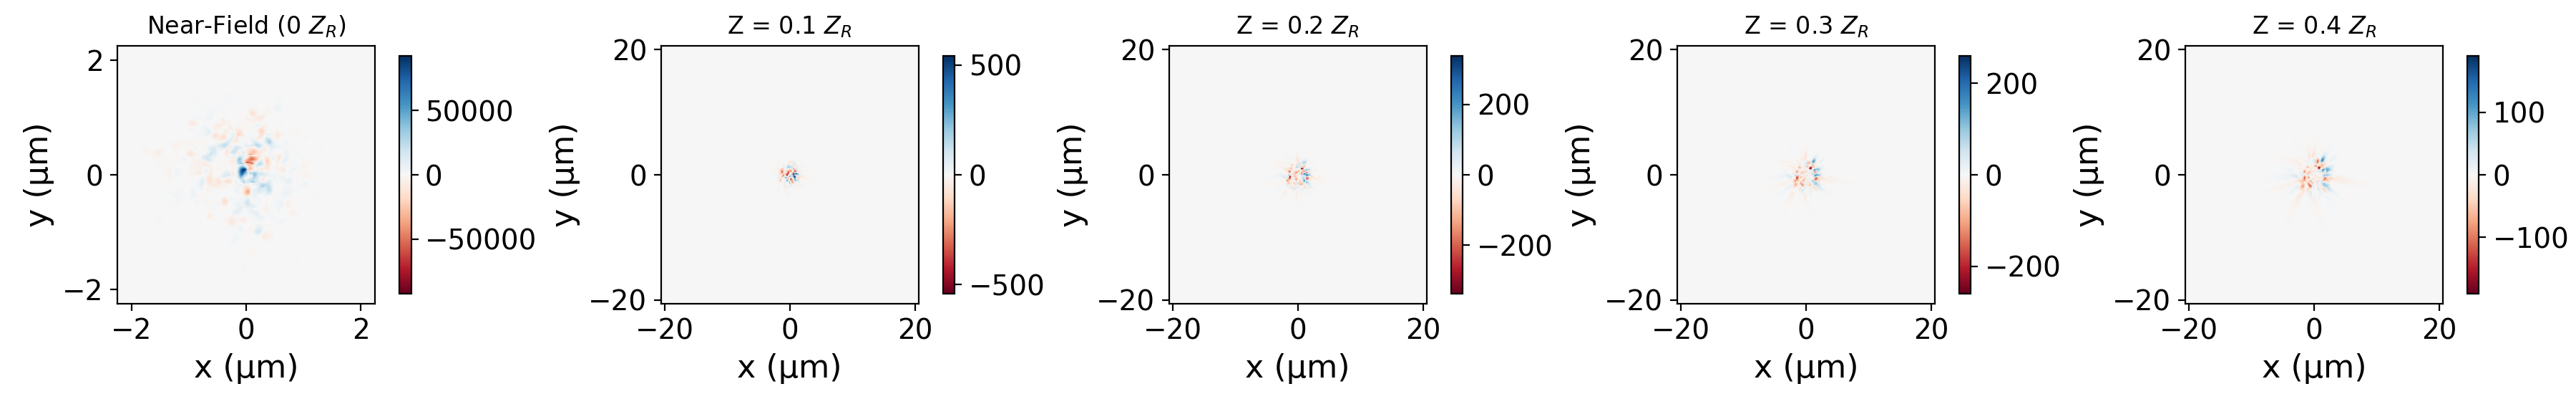
\includegraphics[width=1.0\textwidth]{img/chirality_prop_0p0to0p9zr_Fixed_XY_360_1.png}\\[2pt]
    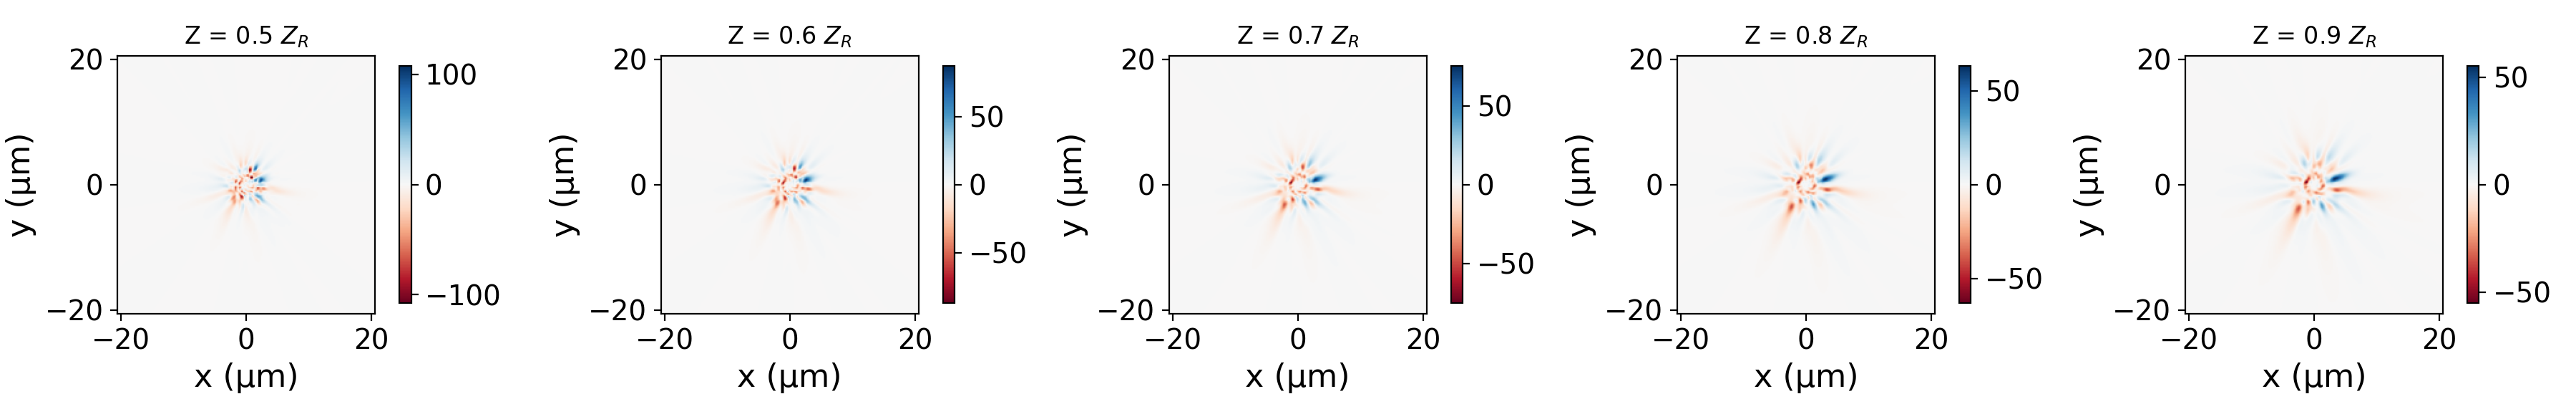
\includegraphics[width=1.0\textwidth]{img/chirality_prop_0p0to0p9zr_Fixed_XY_360_2.png}\\[4pt]
    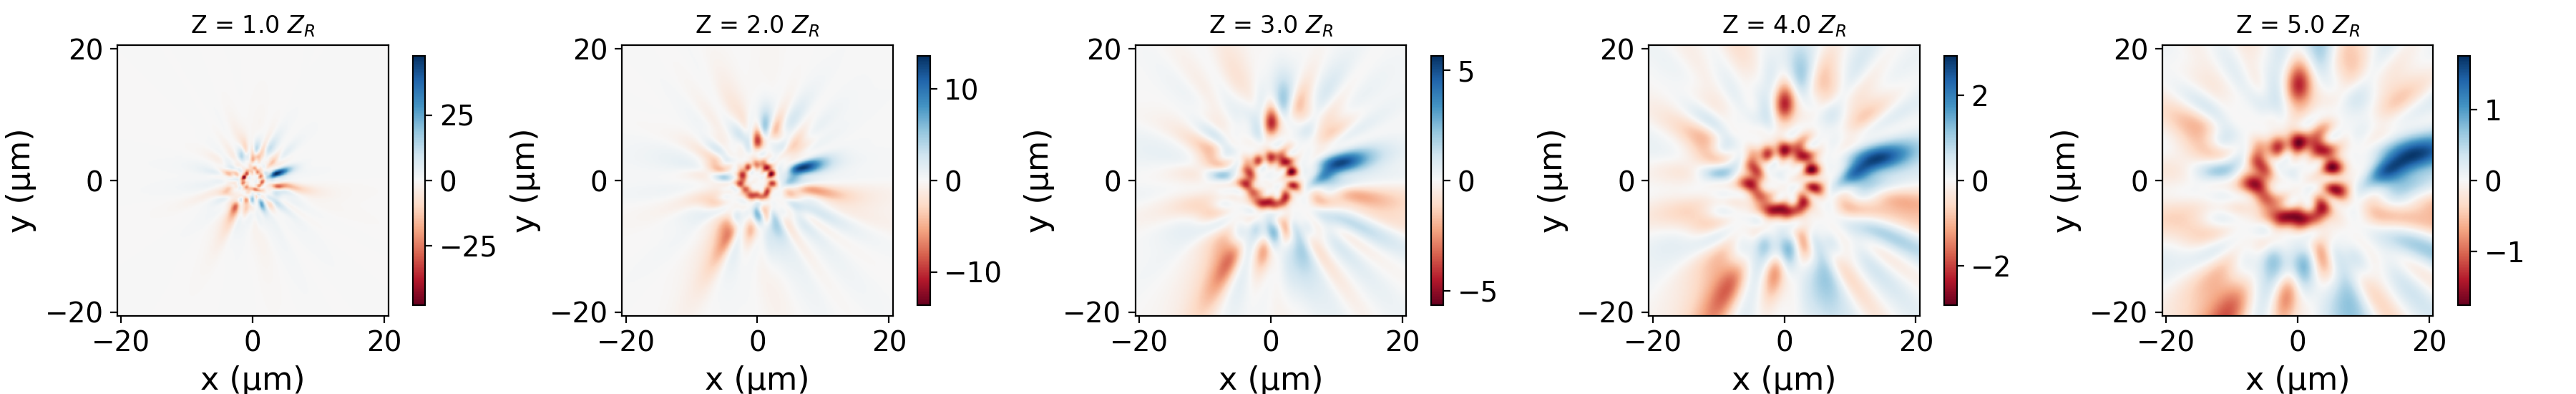
\includegraphics[width=1.0\textwidth]{img/chirality_prop_1to10zr_Fixed_XY_360_1.png}\\[2pt]
    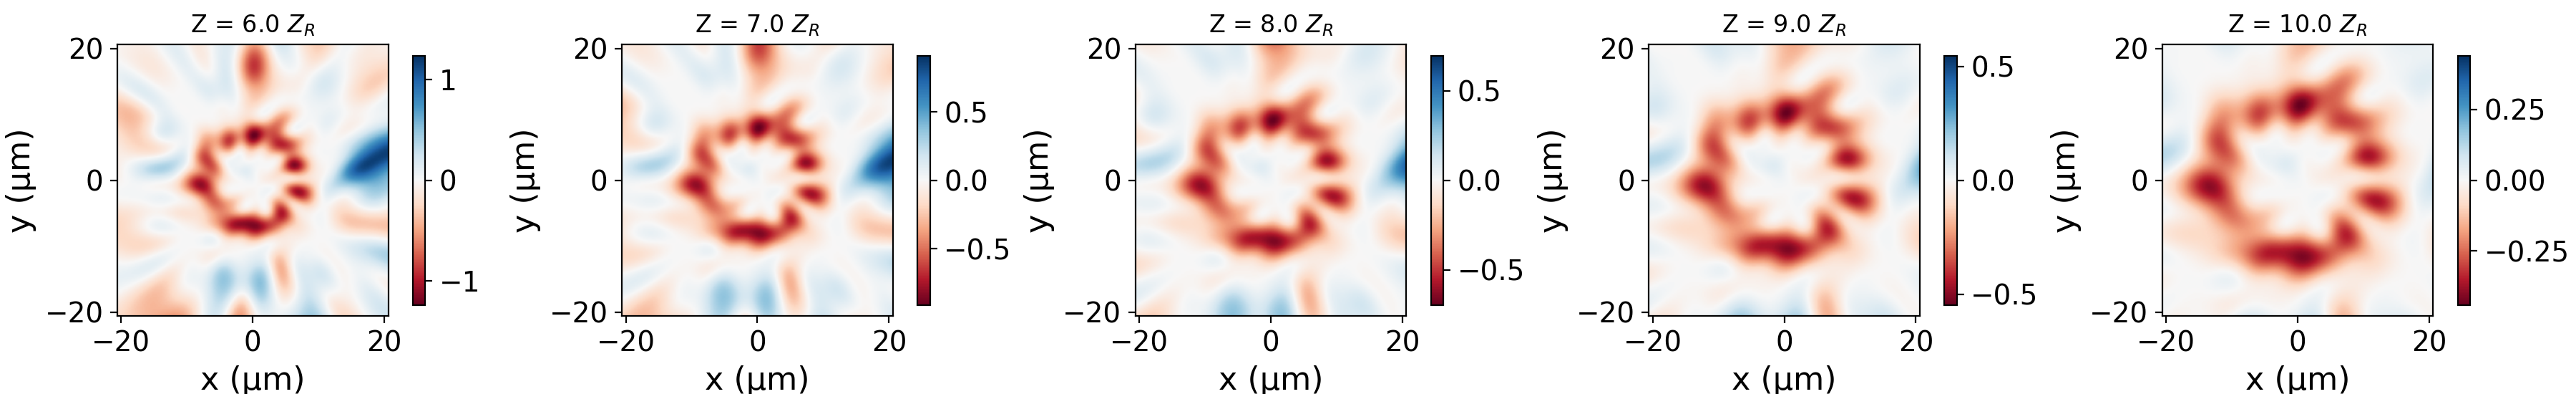
\includegraphics[width=1.0\textwidth]{img/chirality_prop_1to10zr_Fixed_XY_360_2.png}
\caption{Optical chirality propagation evolution for $\ell = 5$. Upper two rows: $z = 0.0z_{R}$ to $0.9z_{R}$; lower two rows: $z = 1.0z_{R}$ to $10.0z_{R}$. Color scale: blue ($C > 0$) indicates RCP dominance; red ($C < 0$) indicates LCP dominance. Near-field scattering creates a mixed LCP/RCP state; by $z \ge z_R$ the field is dominated by the LCP propagating mode.}
\label{fig:chirality_prop}
\end{figure}


\subsection{Near-Field Chirality}
\label{ssec:chirality_near}

Based on the propagation mechanism described above, Figure~\ref{fig:near_chirality_all} further shows the optical chirality density distributions (raw value $C$ and normalized value $C/|C|_\text{max}$) at the near-field monitor plane just above the design layer for $\ell = 0$ to $5$.

In the near-field region, the optical chirality shows a mixed LCP/RCP distribution, with a large fraction of the area exhibiting blue positive values ($C > 0$, i.e., RCP). This arises from the intense local scattering and evanescent wave coupling that the nanostructure induces in the near field, which generates significant local RCP components superimposed on the LCP-dominated source field.

\begin{figure}[htb]
\centering
	\begin{tabular}{cc} 
	    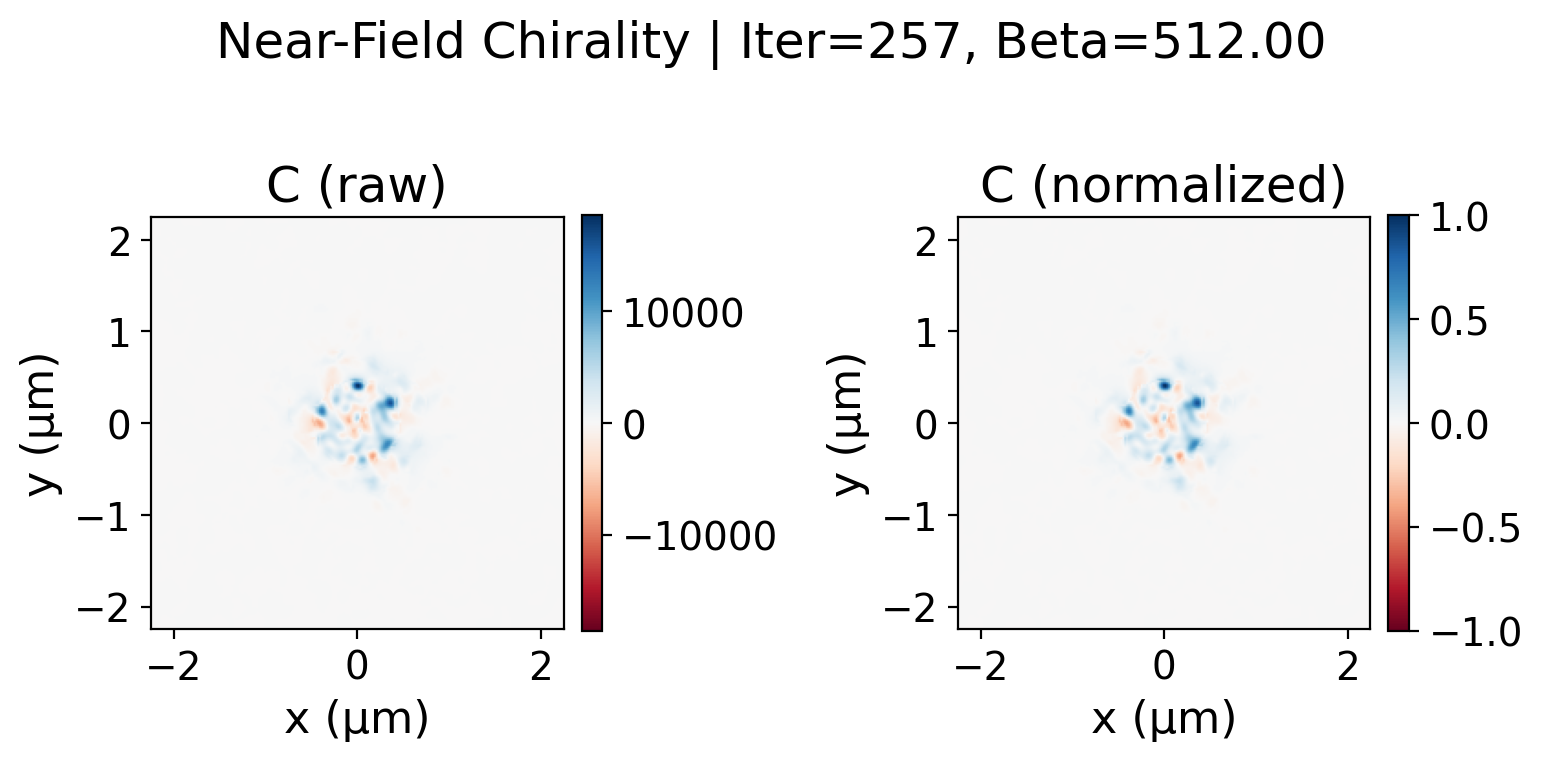
\includegraphics[width=0.47\textwidth]{img/017_near_chirality_257_beta_512.00.png}&
	    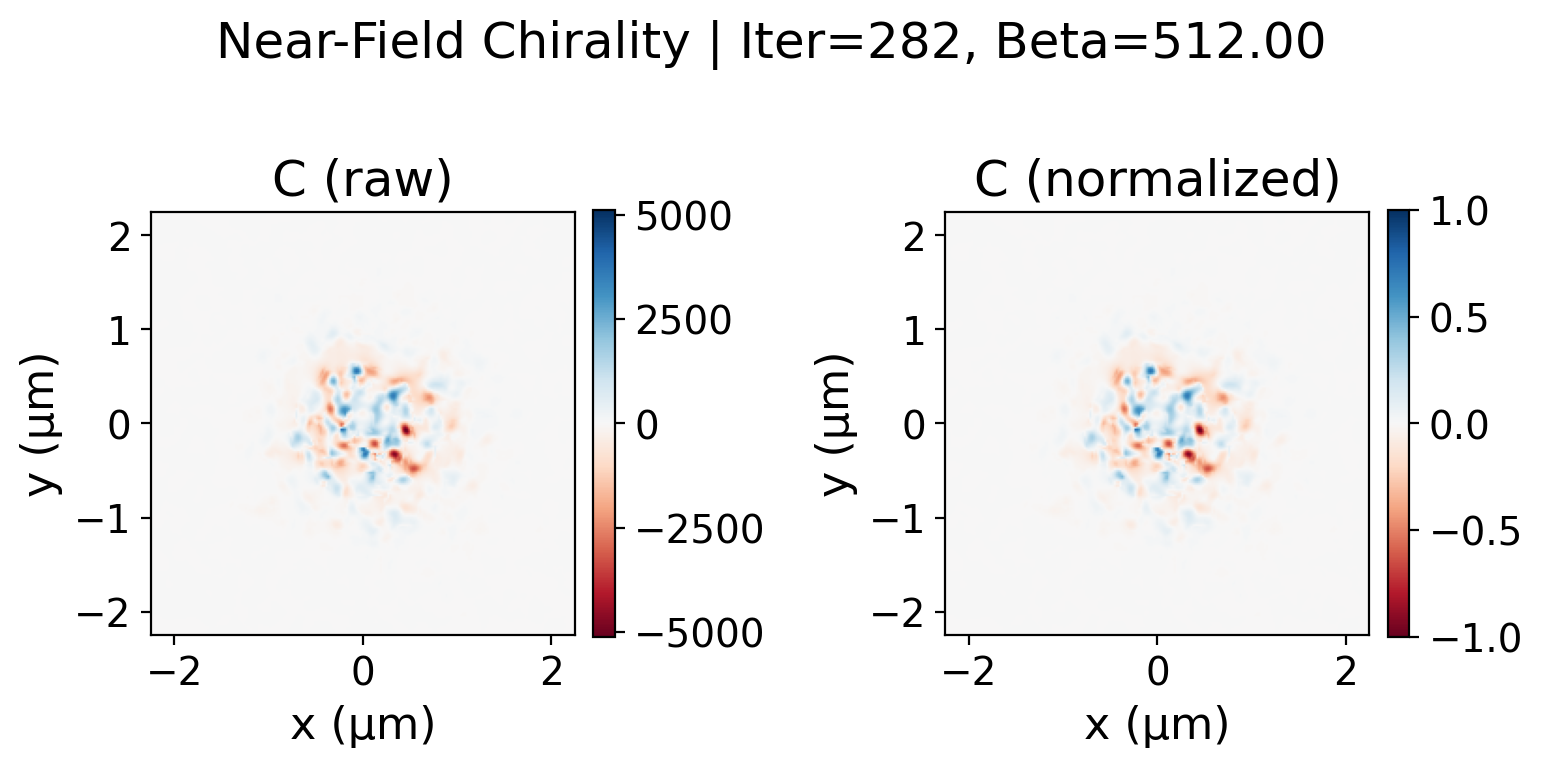
\includegraphics[width=0.47\textwidth]{img/018_near_chirality_282_beta_512.00.png}
		\\ (a) & (b)\\[6pt]
		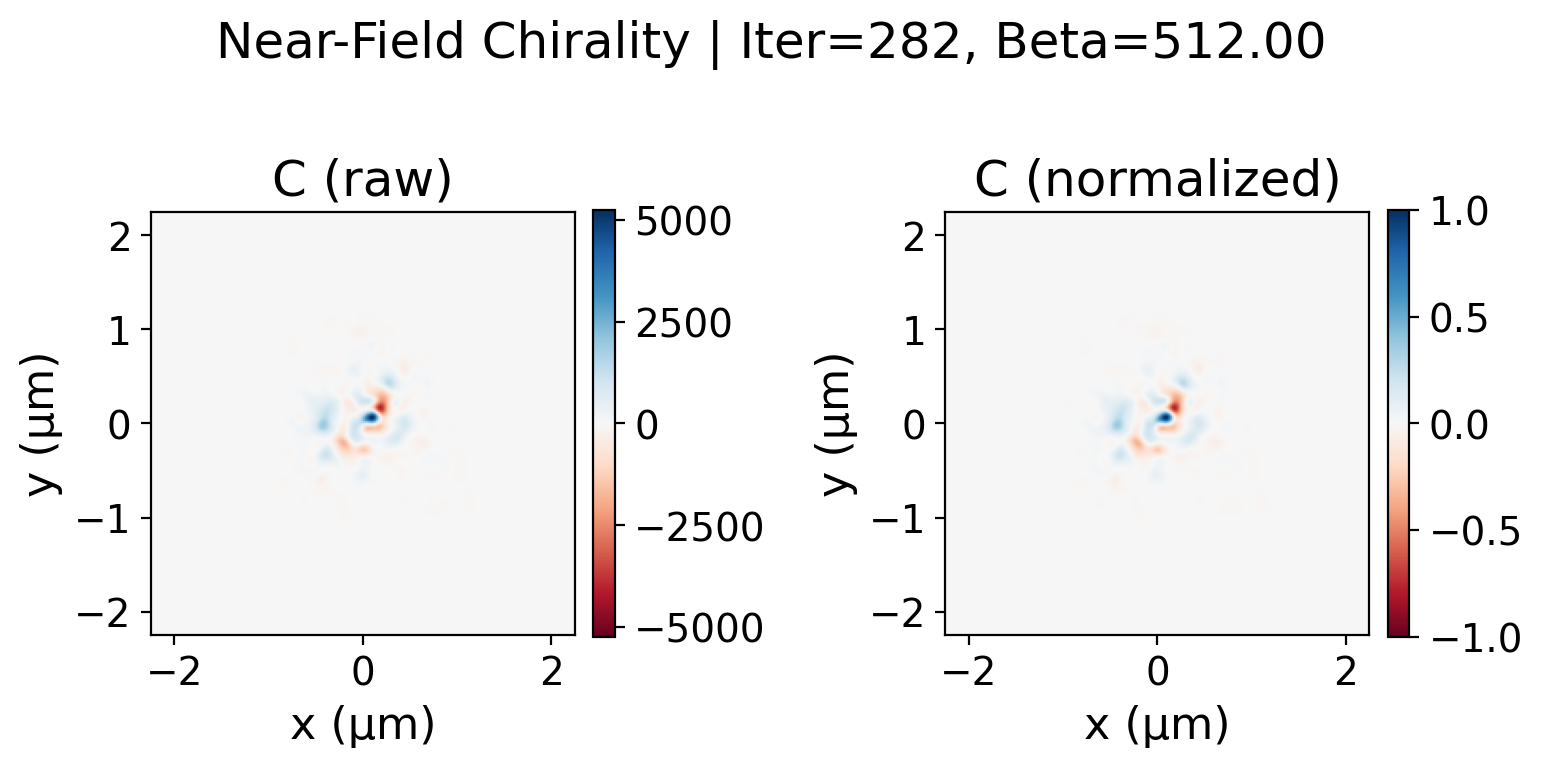
\includegraphics[width=0.47\textwidth]{img/013_near_chirality_282_beta_512.00.png}&
	    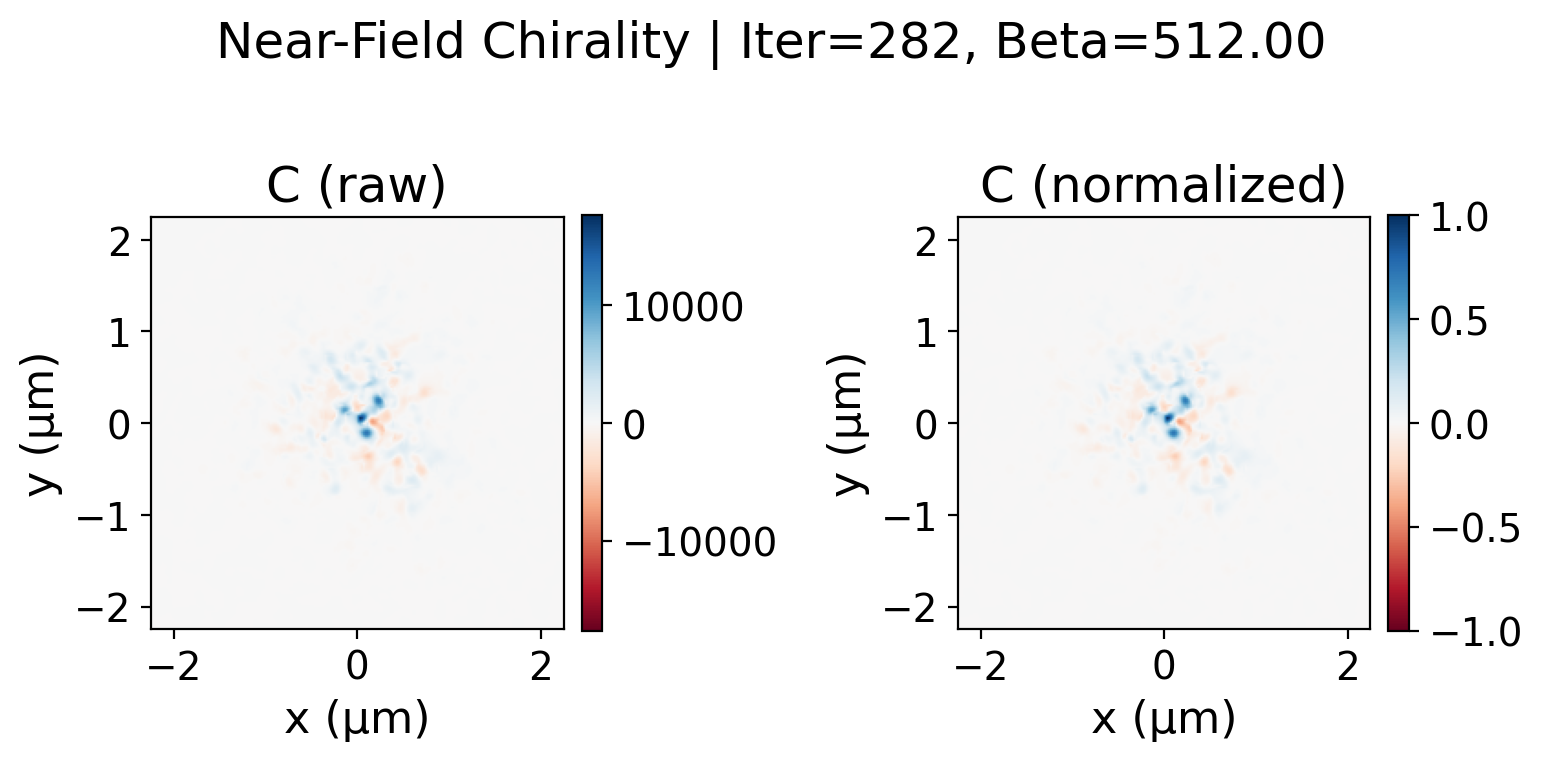
\includegraphics[width=0.47\textwidth]{img/020_near_chirality_282_beta_512.00.png}
	    \\(c) & (d)\\[6pt]
	    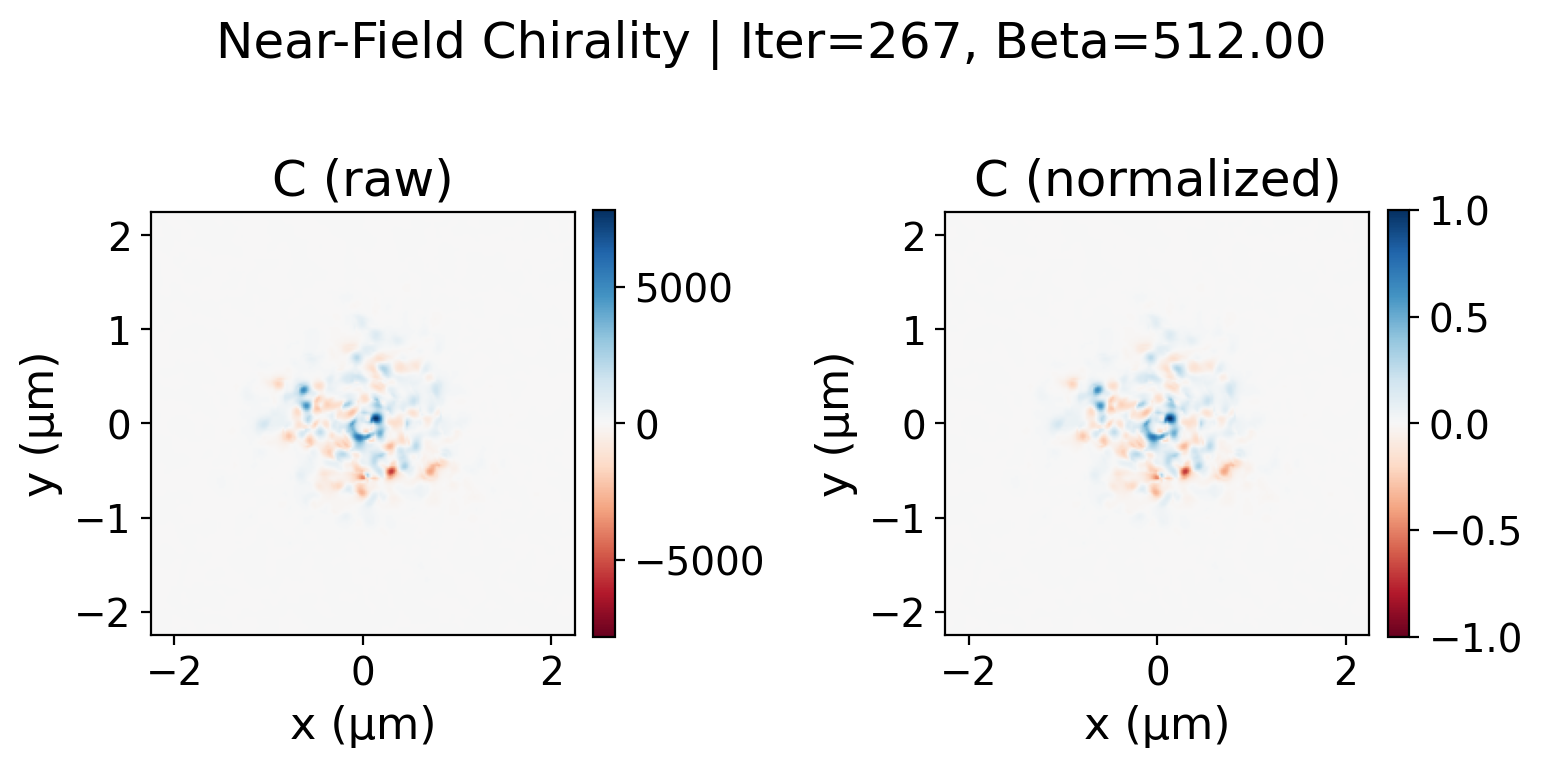
\includegraphics[width=0.47\textwidth]{img/021_near_chirality_267_beta_512.00.png}&
	    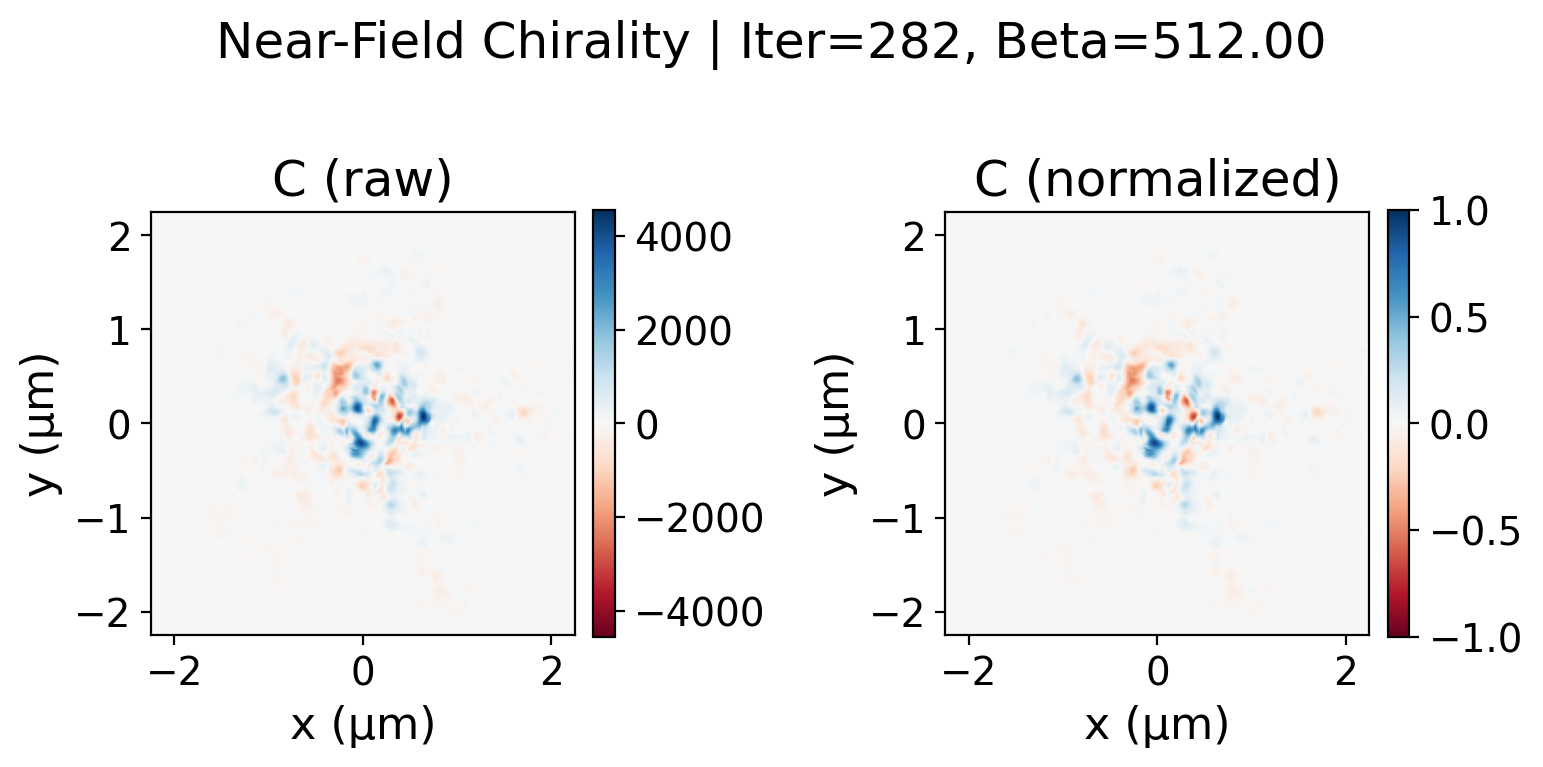
\includegraphics[width=0.47\textwidth]{img/022_near_chirality_282_beta_512.00.png}
	    \\(e) & (f)
	\end{tabular}
\caption{Near-field optical chirality density distributions: (a)$\sim$(f) $\ell \in \{0, 1, 2, 3, 4, 5\}$, respectively. Left column: raw chirality density $C$; right column: normalized chirality density $C/|C|_\text{max}$. The near field shows a mixed LCP/RCP distribution with LCP occupying the majority.}
\label{fig:near_chirality_all}
\end{figure}

\subsection{Far-Field Chirality}
\label{ssec:chirality_far}

Figure~\ref{fig:ff_chirality_all} shows the optical chirality density distributions at the far-field evaluation plane ($z = 10\,z_R$) for $\ell = 0$ to $5$.

Unlike the mixed state in the near field, the far-field chirality density within the main spot region is uniformly and purely negative (red, $C < 0$), meaning the beam has fully recovered to LCP handedness consistent with the K-valley LCP source polarization after propagating to the far field. It is worth noting that the geometric outline of the far-field optical chirality density perfectly overlaps with the far-field intensity distribution. Physically, the chirality distribution closely follows the intensity, confirming that the far-field polarization is highly uniform across the beam cross-section---the beam maintains pure LCP circular polarization everywhere, and the edge decay of the chirality density is only due to intensity falloff, not degradation in polarization quality. This consistent geometric character also indicates that the nanostructure, while performing OAM phase reshaping, effectively decouples spin and orbital angular momentum without introducing unintended spin-orbit coupling effects, ensuring the far-field radiation has very high polarization purity and mode quality.

\begin{figure}[htb]
\centering
	\begin{tabular}{cc} 
	    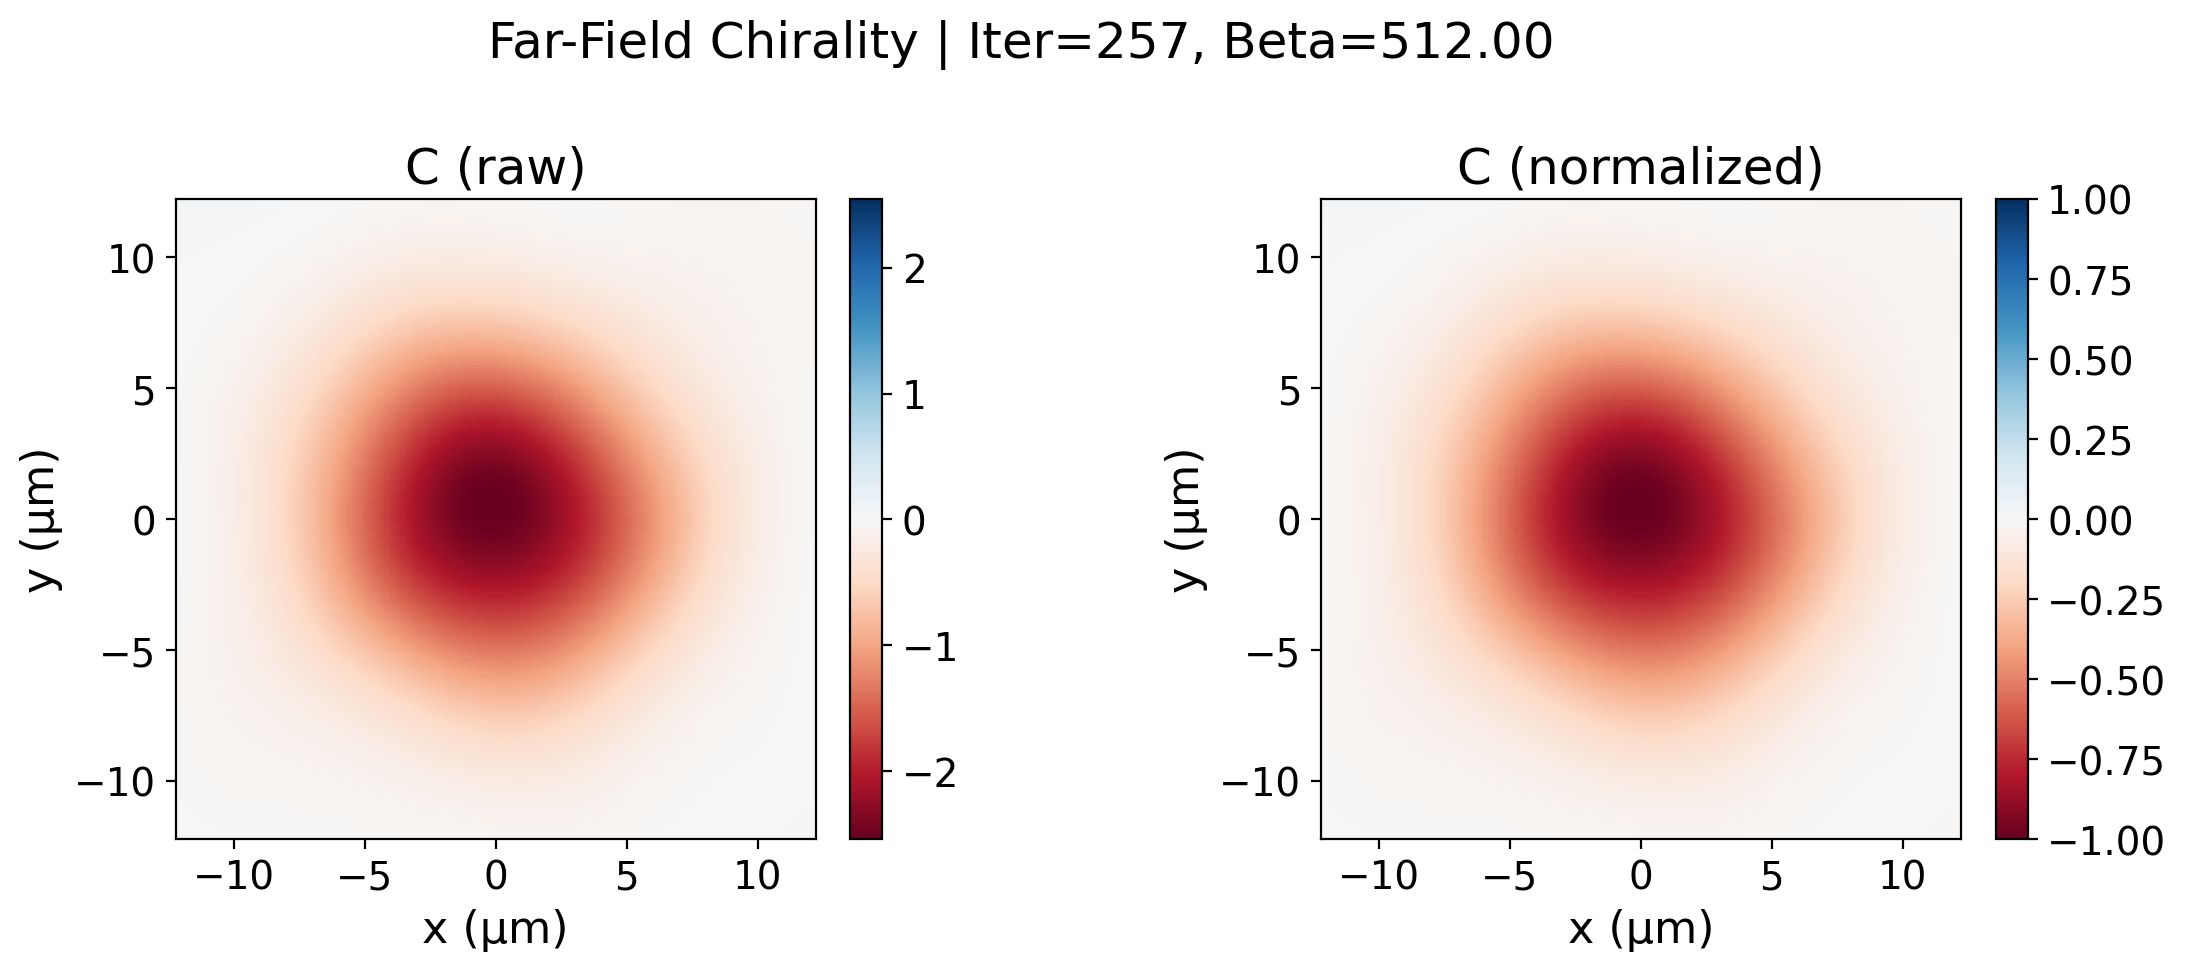
\includegraphics[width=0.47\textwidth]{img/017_ff_chirality_257_beta_512.00.png}&
	    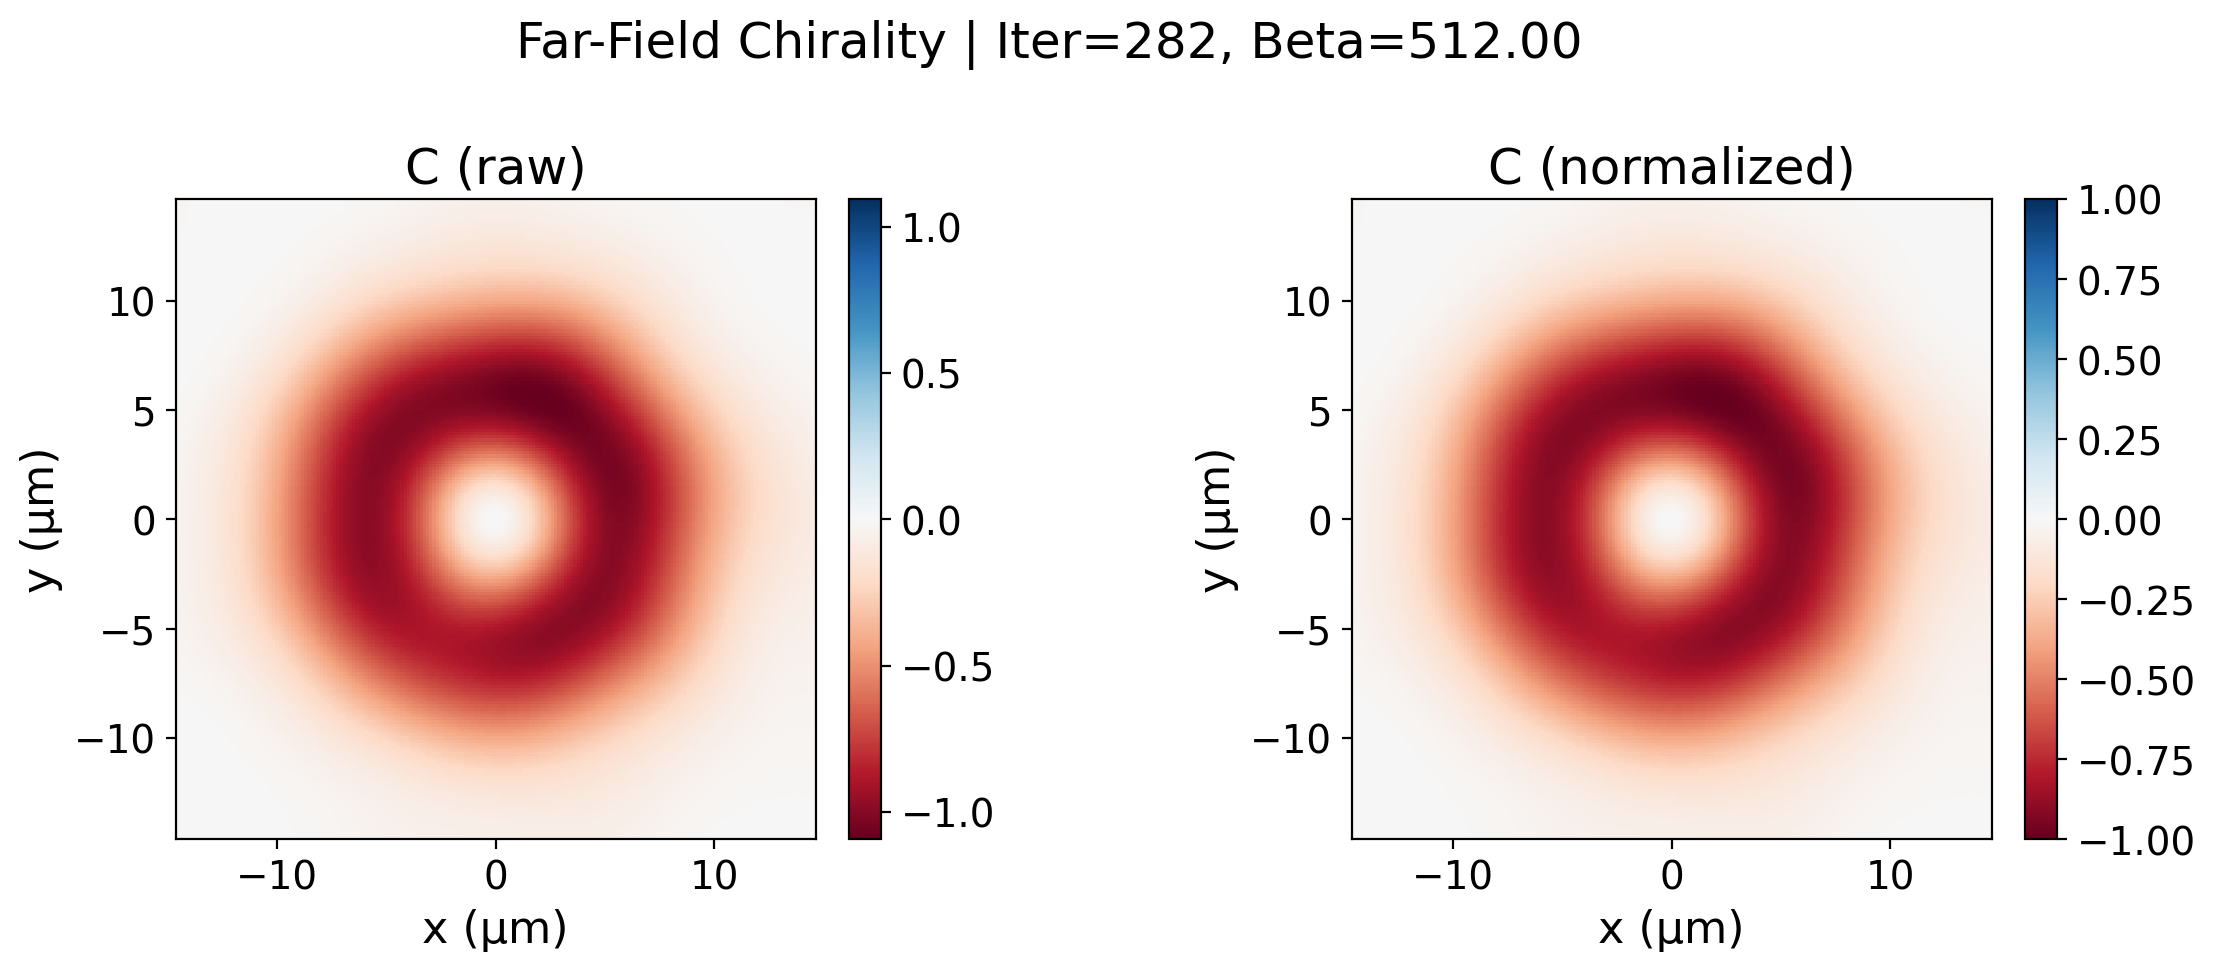
\includegraphics[width=0.47\textwidth]{img/018_ff_chirality_282_beta_512.00.png}
		\\ (a) & (b)\\[6pt]
		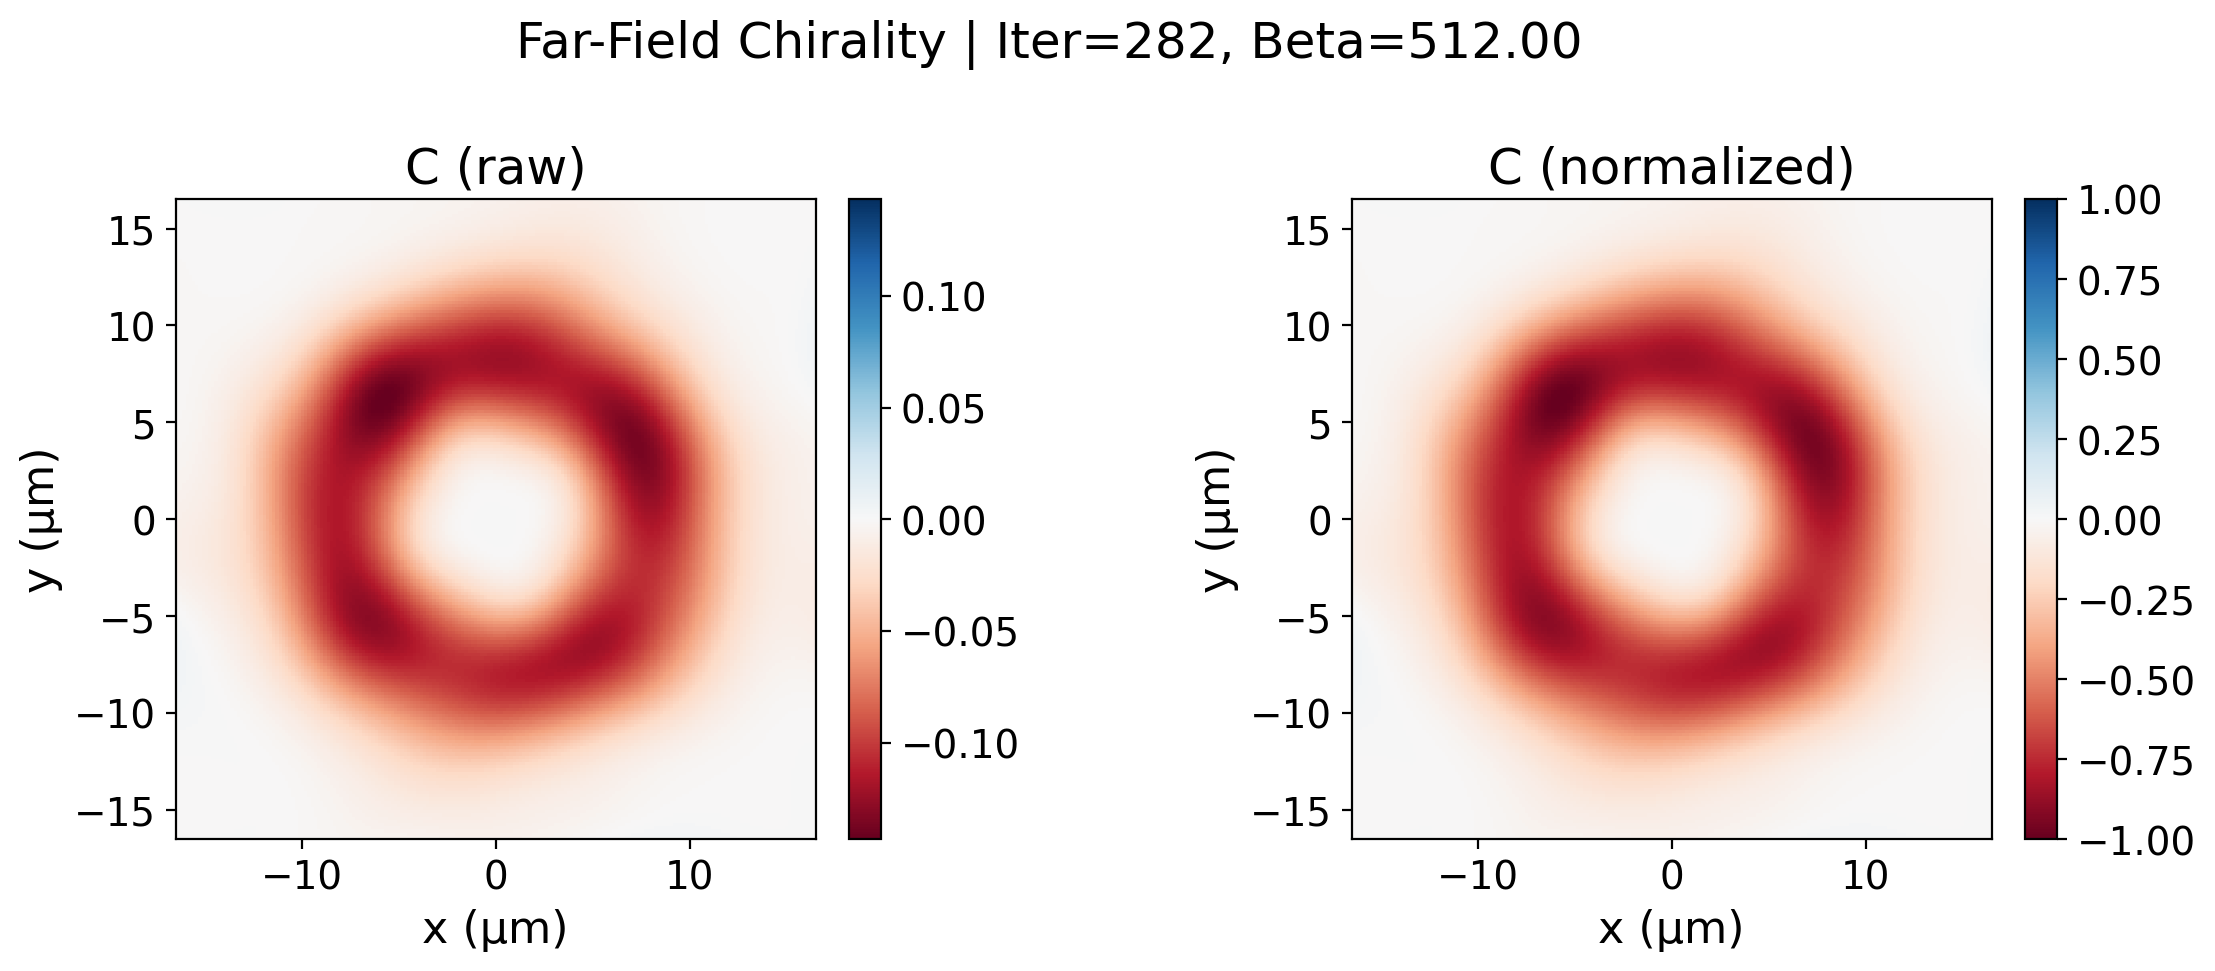
\includegraphics[width=0.47\textwidth]{img/013_ff_chirality_282_beta_512.00.png}&
	    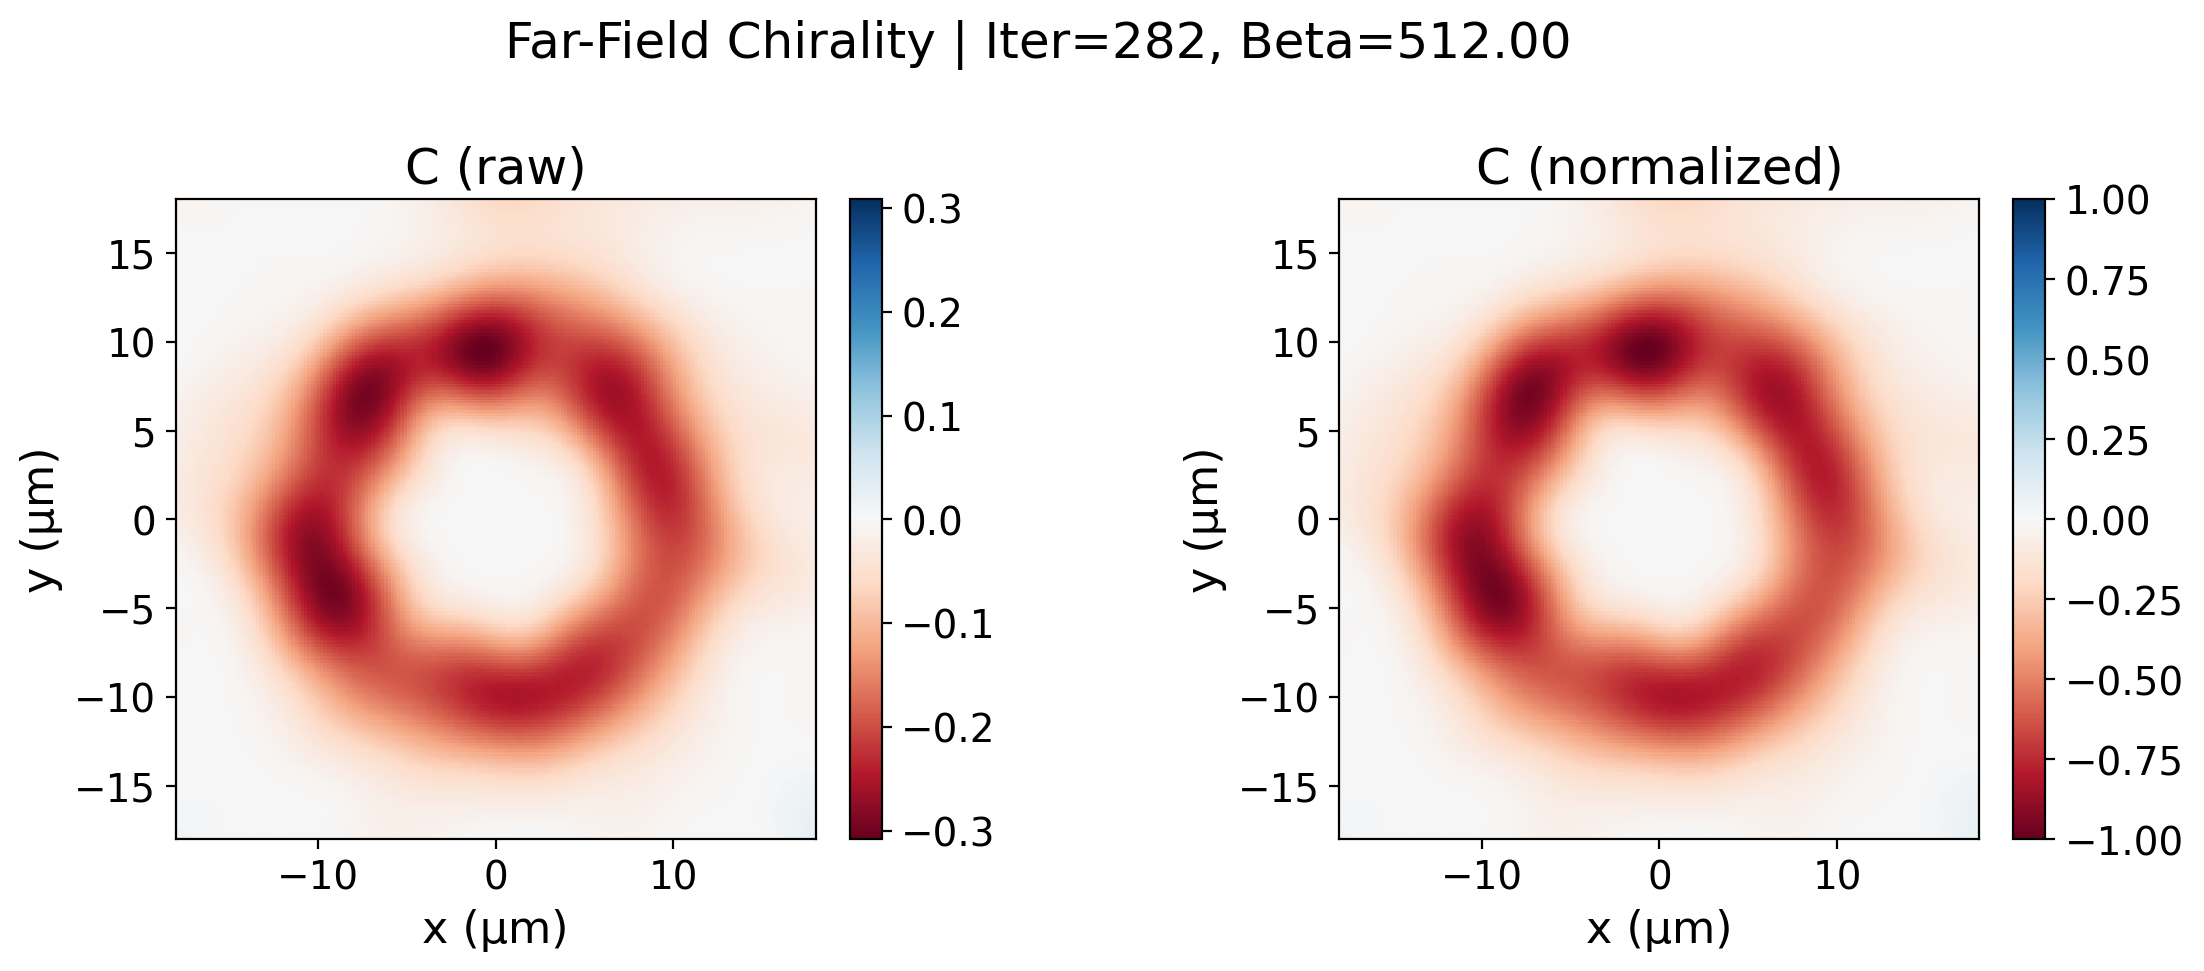
\includegraphics[width=0.47\textwidth]{img/020_ff_chirality_282_beta_512.00.png}
	    \\(c) & (d)\\[6pt]
	    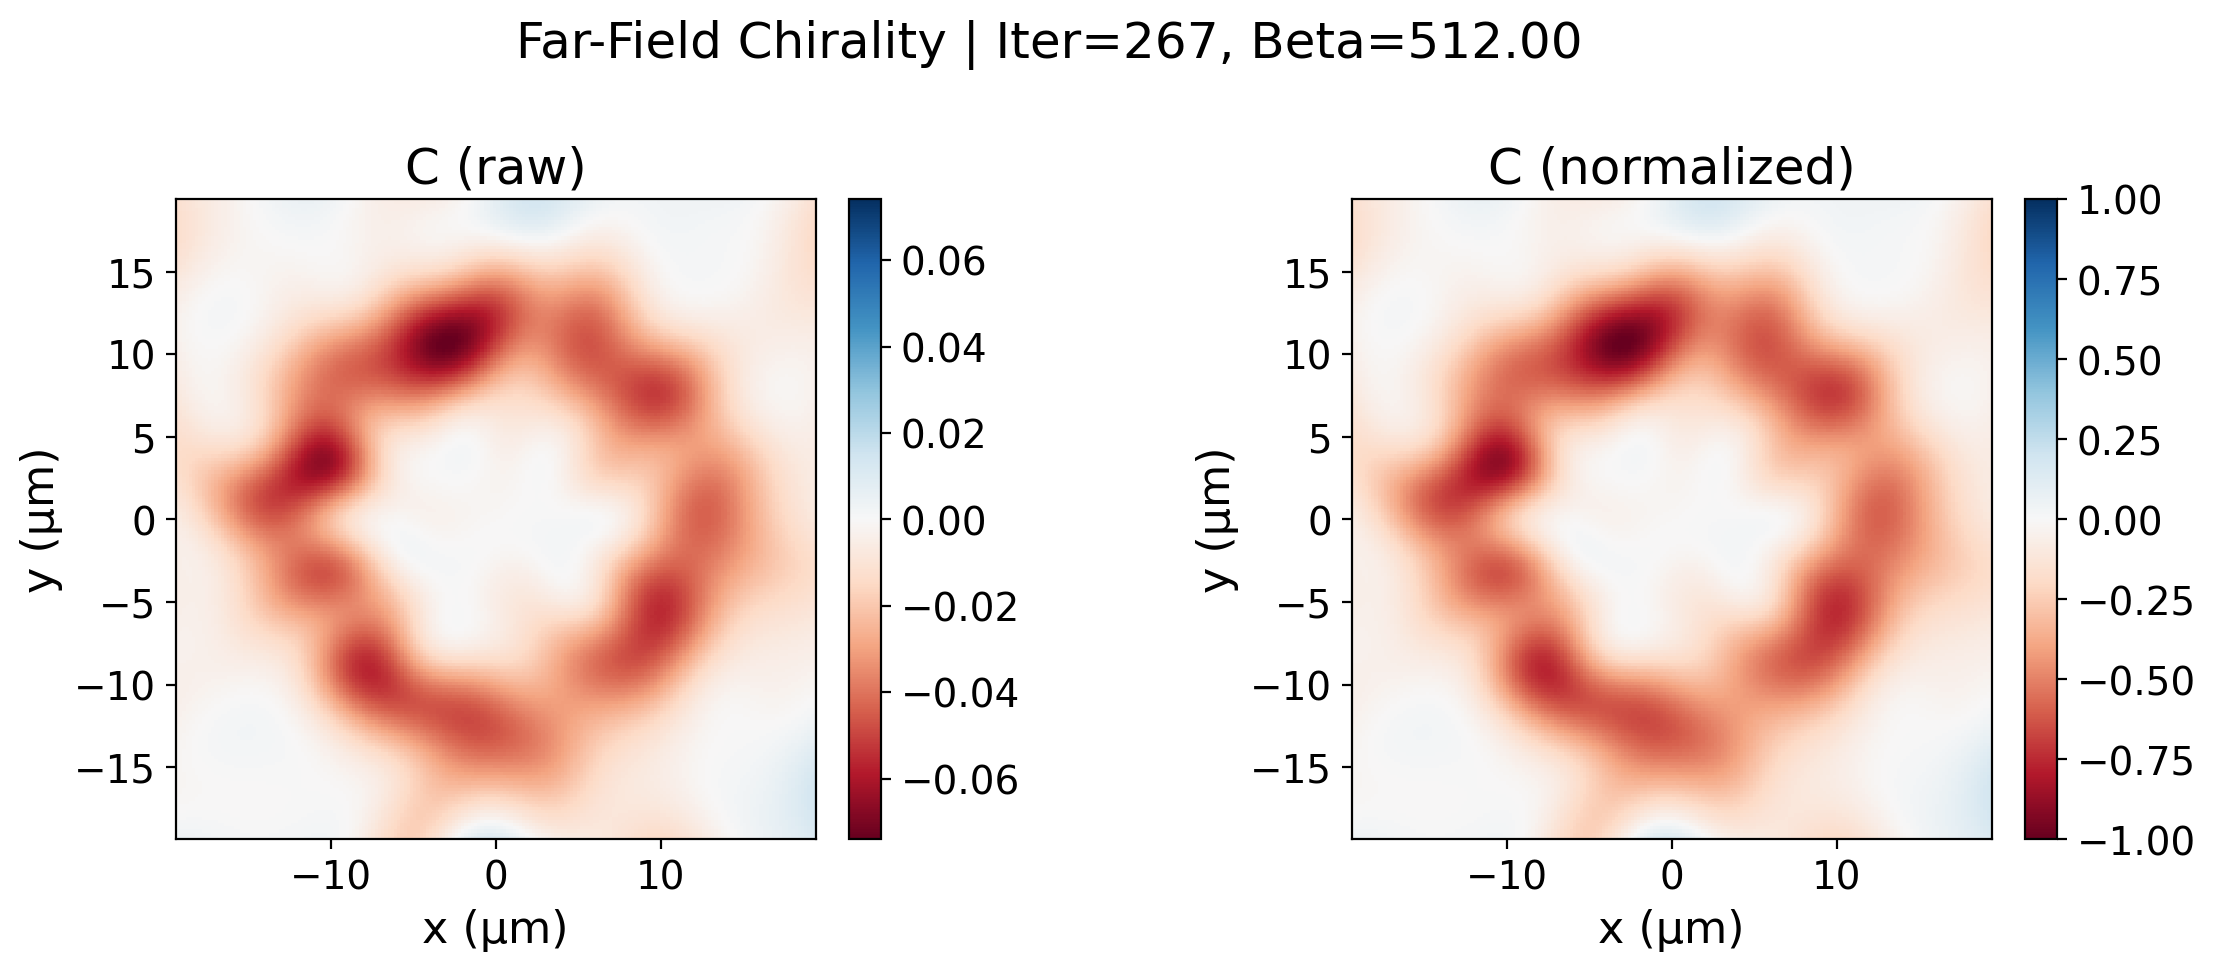
\includegraphics[width=0.47\textwidth]{img/021_ff_chirality_267_beta_512.00.png}&
	    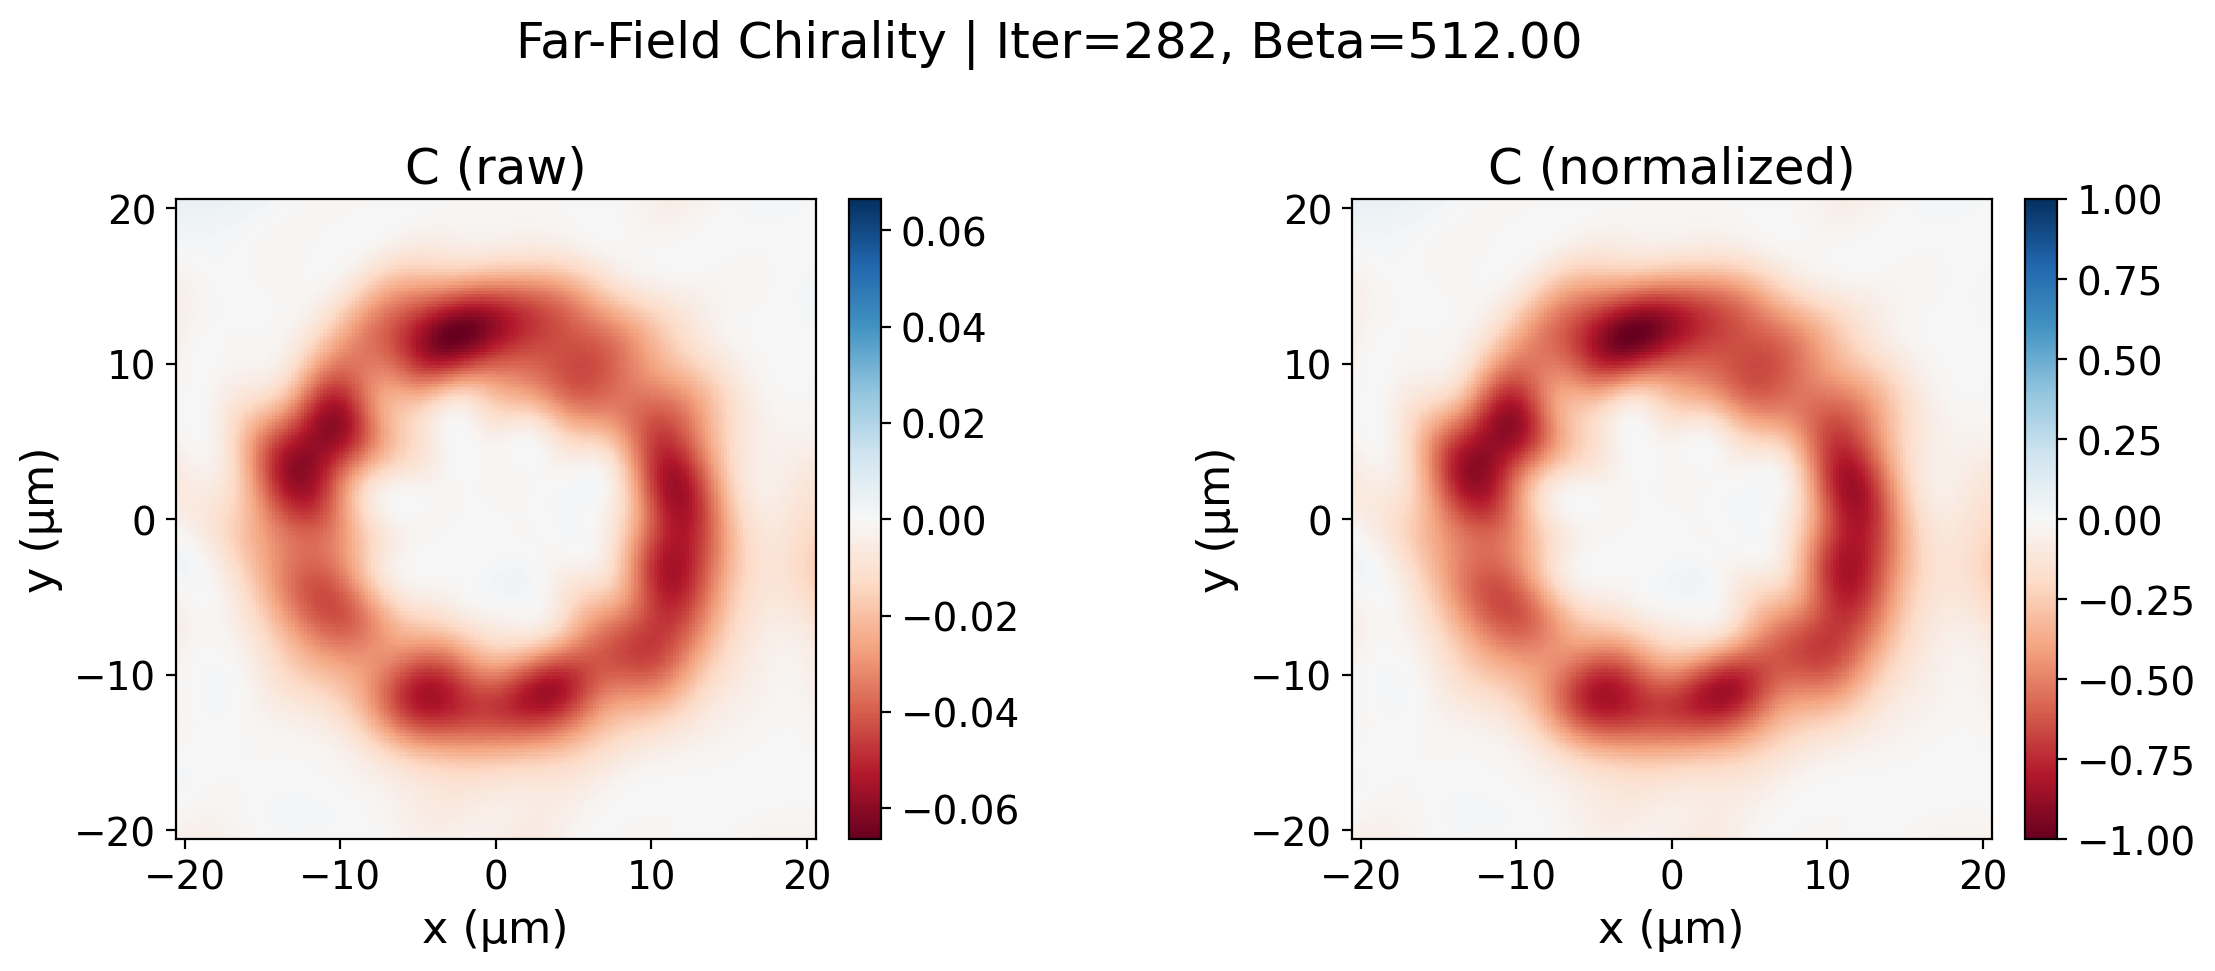
\includegraphics[width=0.47\textwidth]{img/022_ff_chirality_282_beta_512.00.png}
	    \\(e) & (f)
	\end{tabular}
\caption{Far-field optical chirality density distributions ($z = 10\,z_R$): (a)$\sim$(f) $\ell \in \{0, 1, 2, 3, 4, 5\}$, respectively. Left column: raw chirality density $C$; right column: normalized chirality density $C/|C|_\text{max}$. Within the far-field spot, purely uniform RCP (red negative values) chirality is observed.}
\label{fig:ff_chirality_all}
\end{figure}


%===================================================================


\section{Phase Winding Verification}

\label{sec:winding}

Phase winding analysis is the direct method for verifying the topological charge of the far-field vortex beam: the LCP electric field phase is sampled along a circular path at the far-field intensity peak radius $r_\text{peak}$; after unwrapping, the total azimuthal phase change is calculated, which should ideally equal $\ell \times 2\pi$.

Figure~\ref{fig:winding_all} shows the phase winding verification results for the six designs. After sampling along a circular path at the corresponding $r_\text{fraction}$ (ratio of peak radius to evaluation region radius) for each design, the agreement between the unwrapped phase (orange solid line) and the ideal $\ell \times 2\pi$ linear slope (black dashed line) is as follows:
\begin{table}[htb]
\centering
\caption{Phase winding verification results across target topological charges.}
\label{tab:phase_winding}
\begin{tabular}{cccc}
\toprule
$\ell$ & $r_\text{frac}$ & Total Unwrapped Phase & Phase Error \\
\midrule
0 & 0.2000 & $\approx 0 \times 2\pi$ & --- \\
1 & 0.3885 & $1.00 \times 2\pi$ & $< 0.1\%$ \\
2 & 0.4878 & $1.99 \times 2\pi$ & $0.5\%$ \\
3 & 0.5468 & $\approx 3.00 \times 2\pi$ & $< 1\%$ \\
4 & 0.5868 & $\approx 4.00 \times 2\pi$ & $< 1\%$ \\
5 & 0.6176 & $\approx 5.00 \times 2\pi$ & $< 1\%$ \\
\bottomrule
\end{tabular}
\end{table}

The unwrapped phase for all designs closely matches the theoretical prediction, precisely verifying that each design does indeed generate a vortex beam with the target topological charge in the far field. Although the intensity ring for $\ell = 4, 5$ shows slight azimuthal non-uniformity (see Section~\ref{sec:farfield}), the phase winding still accurately reflects the corresponding topological charge. This indicates that the loss of high purity mainly comes from deviations in the intensity profile rather than misalignment of the phase singularity or a change in the topological charge.
\begin{figure}[htb]
\centering
	\begin{tabular}{cc} 
	    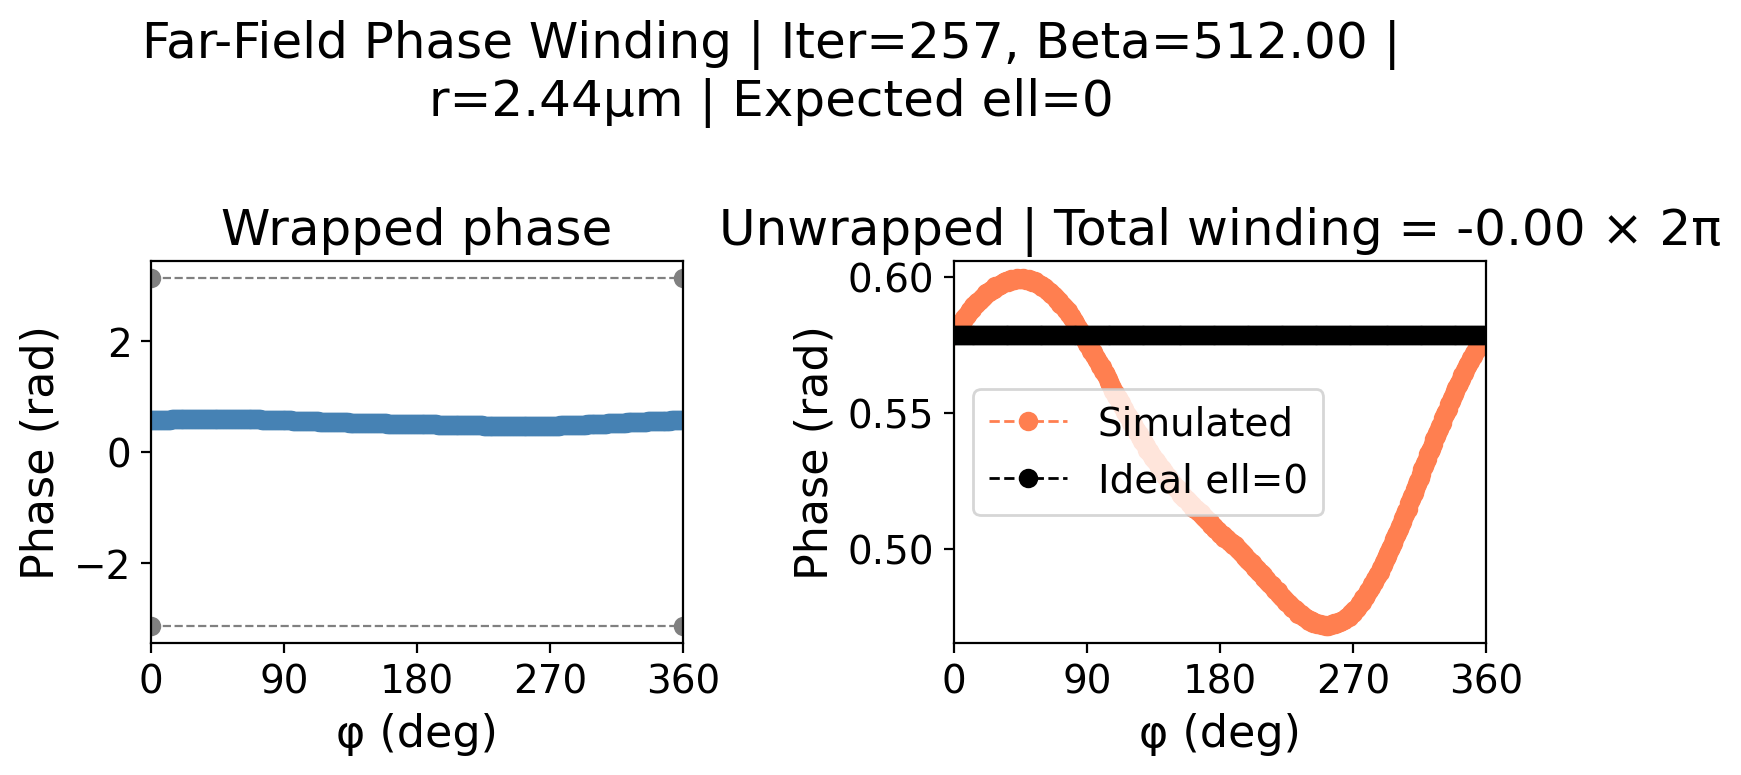
\includegraphics[width=0.47\textwidth]{img/017_ff_winding_iter_257_beta_512.00_rfraction_0.2000.png}&
	    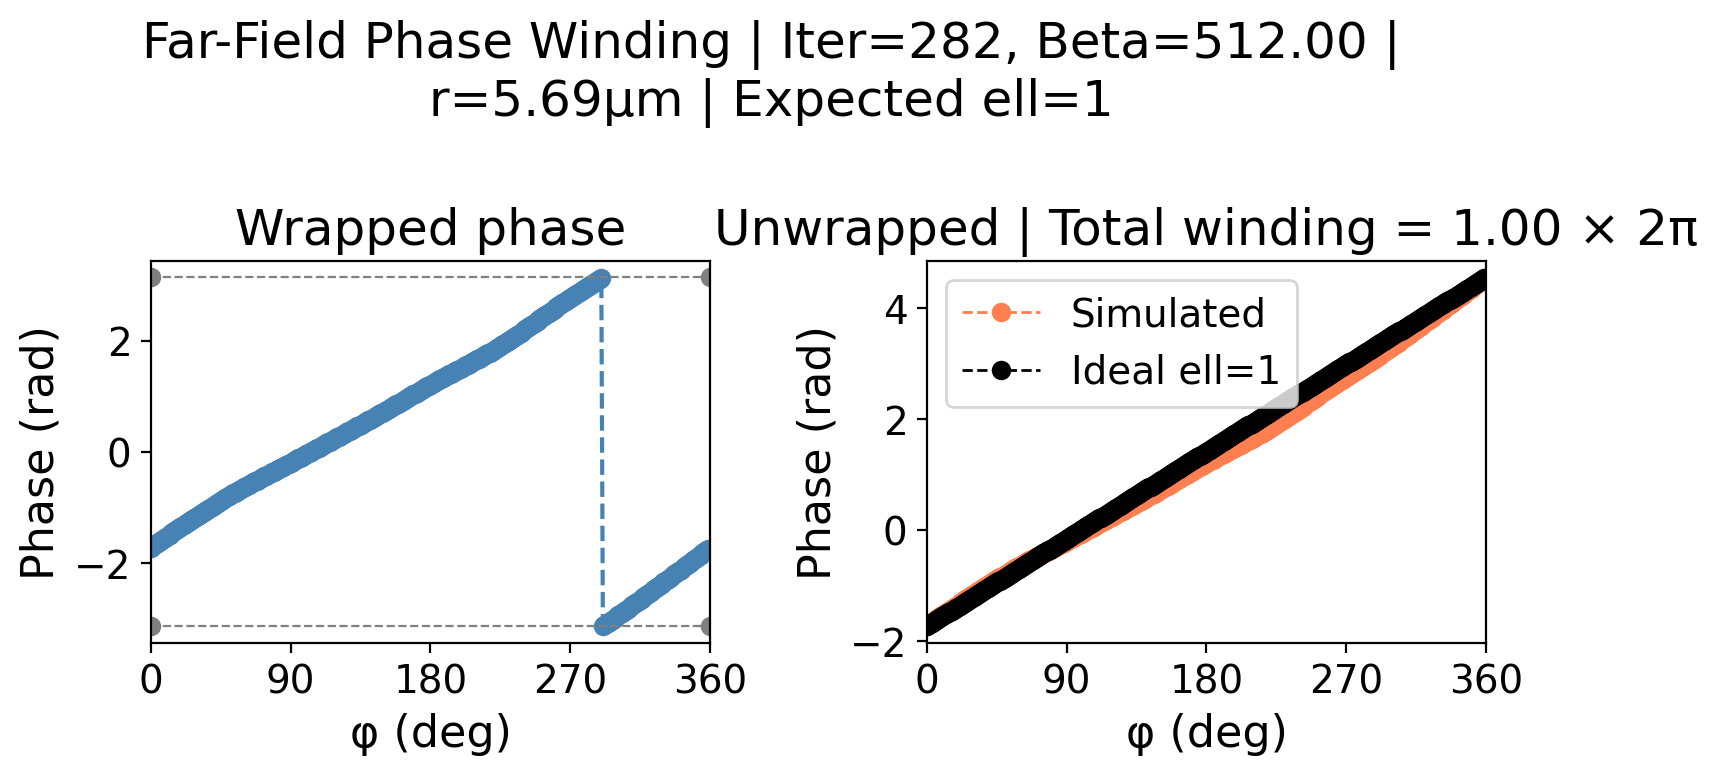
\includegraphics[width=0.47\textwidth]{img/018_ff_winding_iter_282_beta_512.00_rfraction_0.3885.png}
		\\ (a) & (b)\\[6pt]
		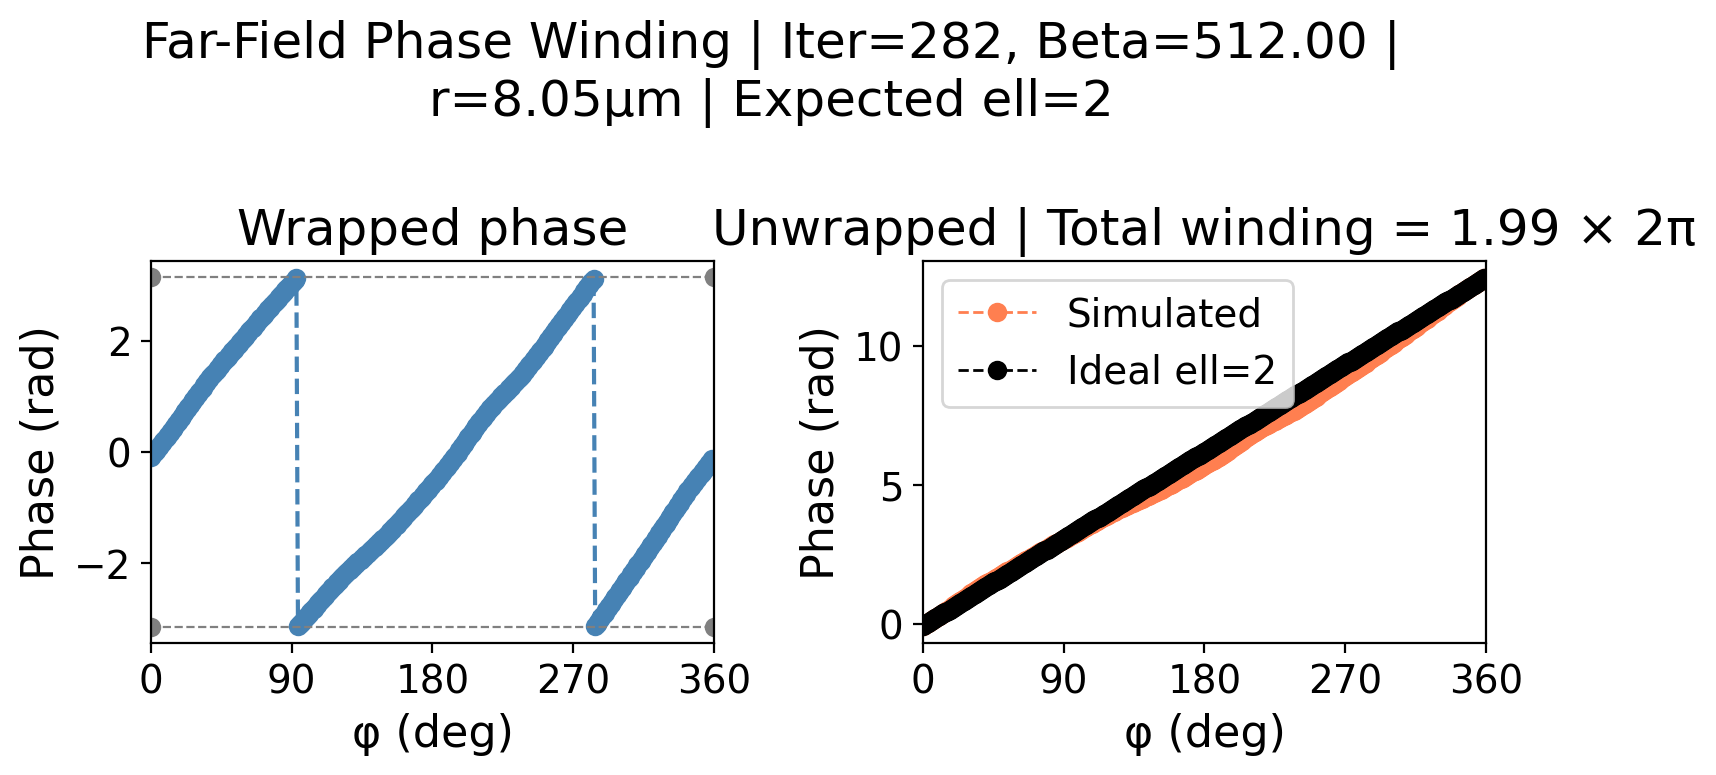
\includegraphics[width=0.47\textwidth]{img/013_ff_winding_iter_282_beta_512.00_rfraction_0.4878.png}&
	    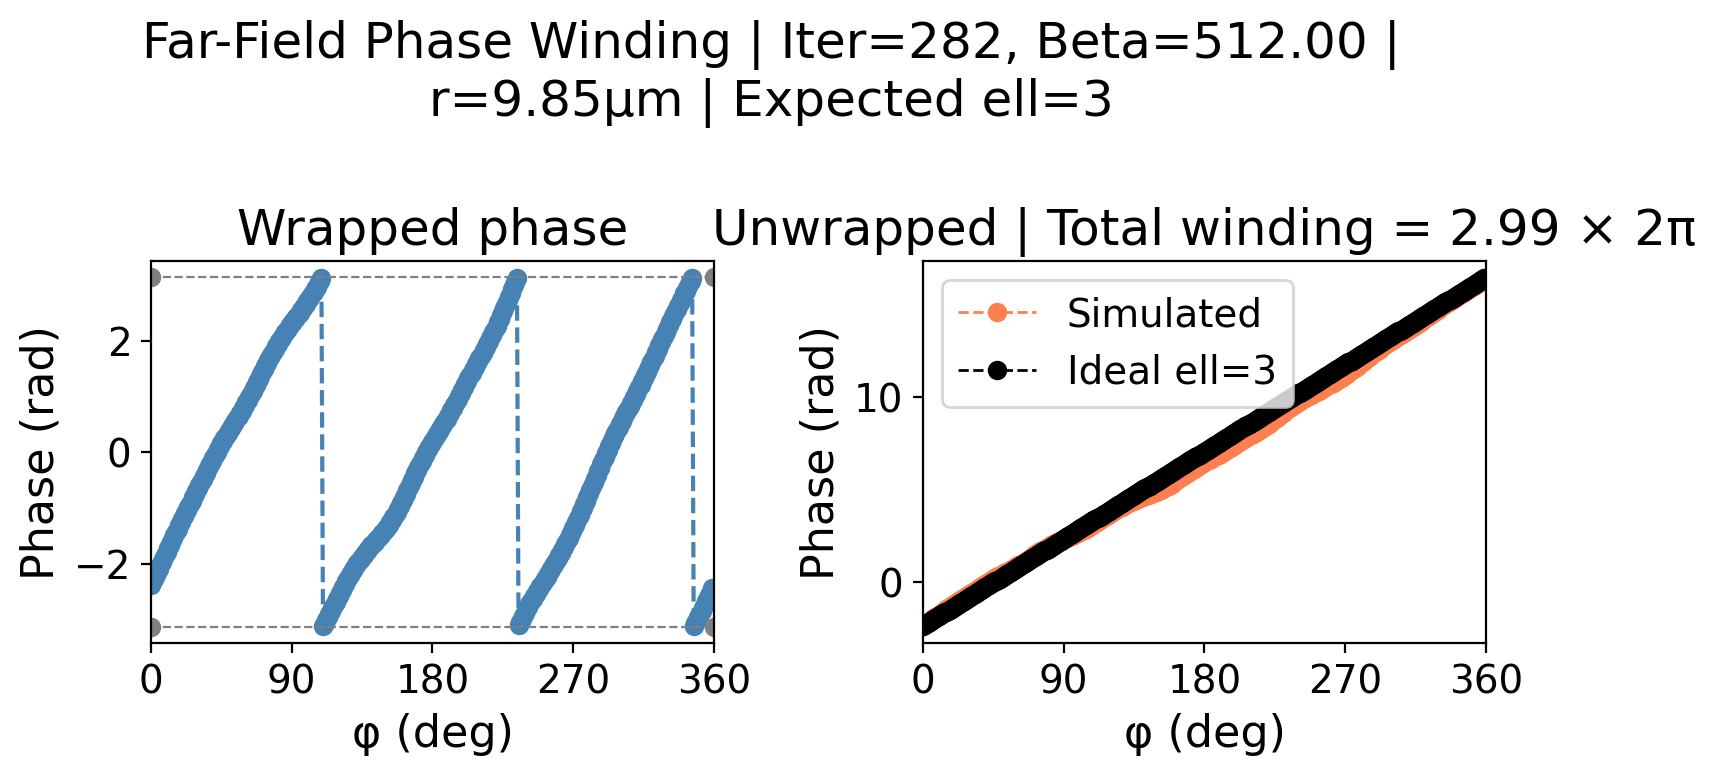
\includegraphics[width=0.47\textwidth]{img/020_ff_winding_iter_282_beta_512.00_rfraction_0.5468.png}
	    \\(c) & (d)\\[6pt]
	    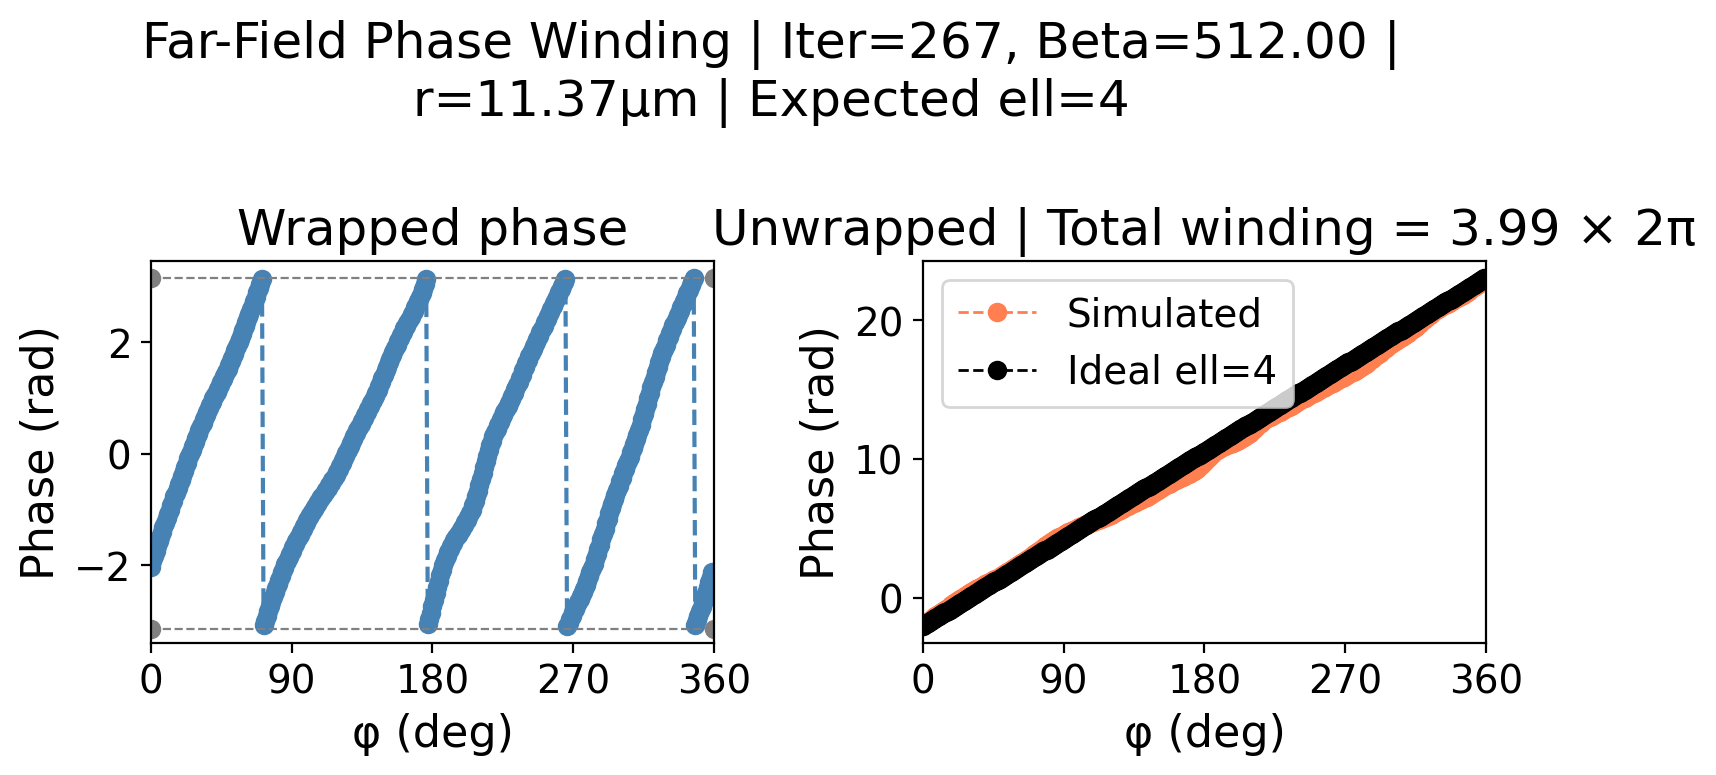
\includegraphics[width=0.47\textwidth]{img/021_ff_winding_iter_267_beta_512.00_rfraction_0.5868.png}&
	    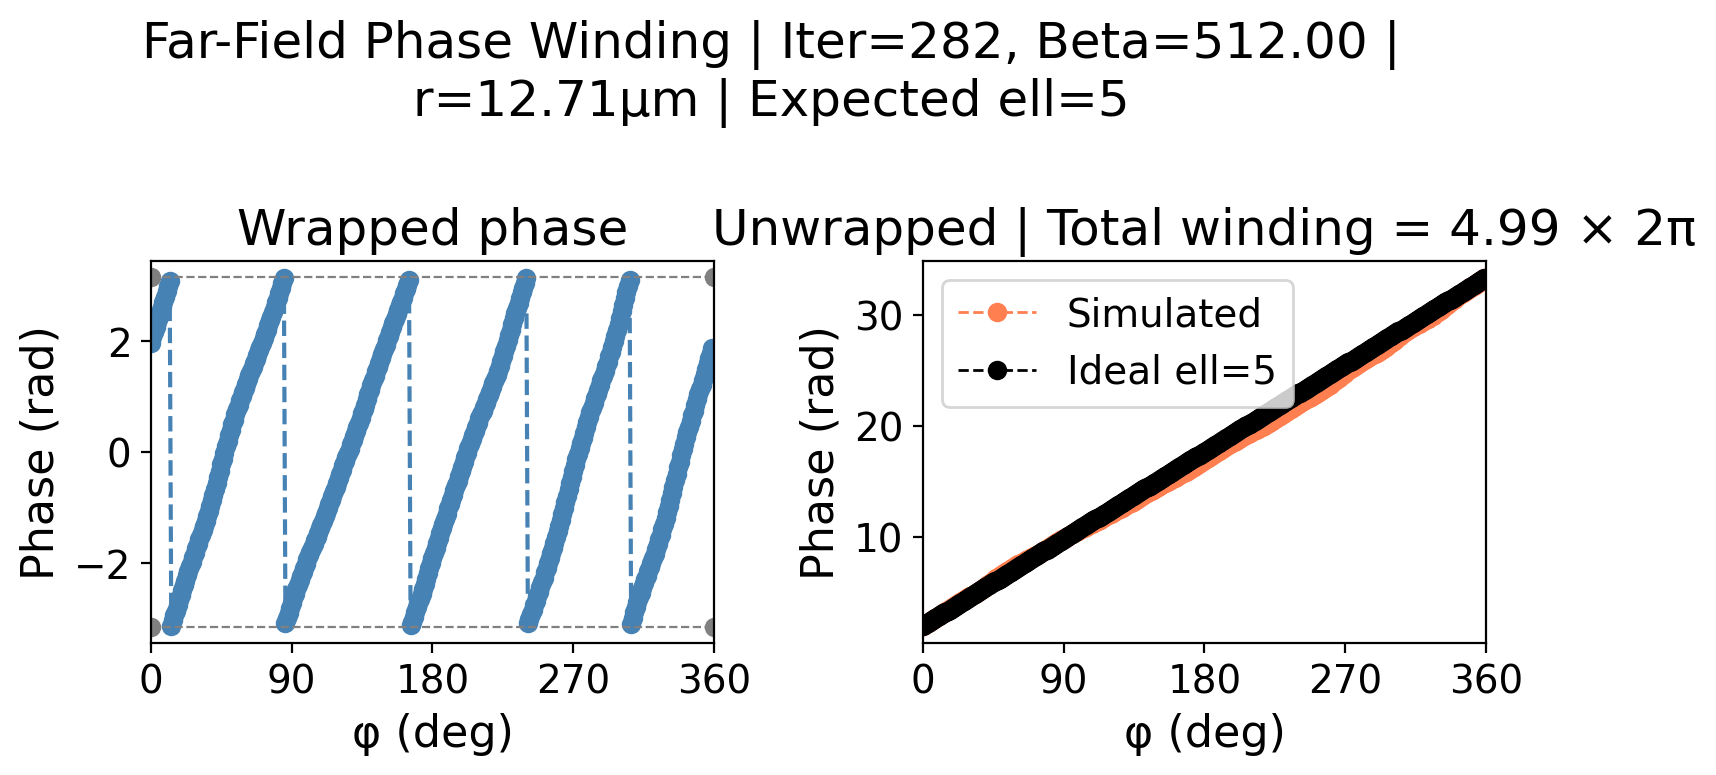
\includegraphics[width=0.47\textwidth]{img/022_ff_winding_iter_282_beta_512.00_rfraction_0.6176.png}
	    \\(e) & (f)
	\end{tabular}
\caption{Far-field phase winding verification: (a)$\sim$(f) $\ell \in \{0, 1, 2, 3, 4, 5\}$, respectively. Sub-panel left column: wrapped phase sampled azimuthally at the peak radius; sub-panel right column: unwrapped phase (orange) compared with the ideal $\ell \times 2\pi$ slope (black dashed line). For all designs, the total unwrapped phase agrees with the target topological charge to within $< 1\%$ error.}
\label{fig:winding_all}
\end{figure}

%===================================================================


\section{Circular Polarization Selectivity}
\label{sec:pol_selectivity}
To confirm whether the optimized nanostructure can accurately distinguish polarization states, a cross-polarization excitation test is performed in this section. In valleytronics applications, the $K$-valley and $K'$-valley excitons in a WS$_2$ monolayer emit LCP and RCP light respectively; therefore, the structure must be able to recognize a specific polarization state while suppressing coupling to the non-target polarization.

All topological structures were topology-optimized using an LCP point source. To quantitatively examine their selectivity, all five non-Gaussian designs ($\ell = 1$ to $5$) were tested: the input source is changed to an RCP point source of opposite handedness, and the far-field OAM mode purity as well as $|\text{Overlap}|^2$ are evaluated for each structure.

The results are summarized in Table~\ref{tab:rcp_selectivity}. In all five cases, the RCP-excited far-field purity of the target mode collapses to near-zero values: $\ell = 1, 3$ give $0.03\%$, while $\ell = 2, 4, 5$ all round to $0.00\%$ (actual values $< 0.005\%$). The $|\text{Overlap}|^2$ values are likewise indistinguishable from zero for all designs. These results stand in sharp contrast to the high-purity LCP-excited performance listed in Table~\ref{tab:results_summary} ($82\%$--$99\%$), directly demonstrating that every LCP-optimized structure exhibits extremely strong circular polarization selectivity.

\begin{table}[htb]
\centering
\caption{RCP cross-polarization excitation test results for $\ell = 1$ to $5$ (far-field plane at $z = 10\,z_R$). Values are rounded to two decimal places; entries showing $0.00$ indicate actual values $< 0.005$.}
\label{tab:rcp_selectivity}
    \begin{tabular}{cccc}
        \hline
        $\ell$ & LCP Purity (\%) & RCP Purity (\%) & Valley Contrast Ratio\\
        \hline
        1 & 98.66 & 0.03 & $\approx 3289:1$\\
        2 & 97.96 & 0.00 & $> 19592:1$\\
        3 & 94.13 & 0.03 & $\approx 3138:1$\\
        4 & 81.94 & 0.00 & $> 16388:1$\\
        5 & 82.62 & 0.00 & $> 16524:1$\\
        \hline
    \end{tabular}
\end{table}

For the representative case of $\ell = 3$ (purity $94.13\%$ vs.\ $0.03\%$), the valley contrast ratio reaches approximately $3138:1$, establishing a clear and directly experimentally benchmarkable inter-valley discrimination baseline. The contrast is even larger for $\ell = 2, 4, 5$, where the RCP purity is below the rounding threshold.

This polarization selectivity arises from the geometric phase and near-field asymmetric scattering within the nanostructure. When the non-target polarization (RCP) is incident, the structure cannot satisfy the geometric phase conditions required for OAM mode shaping, and the vast majority of the energy is scattered into stray fields that cannot effectively couple into the far-field target mode.

Figure~\ref{fig:ff_purity_rcp} shows the far-field results for all five designs under RCP excitation alongside their LCP reference, confirming that no recognizable OAM ring or spiral phase structure is recovered in any case.

\begin{figure}[htb]
\centering
    \begin{tabular}{ccc}
        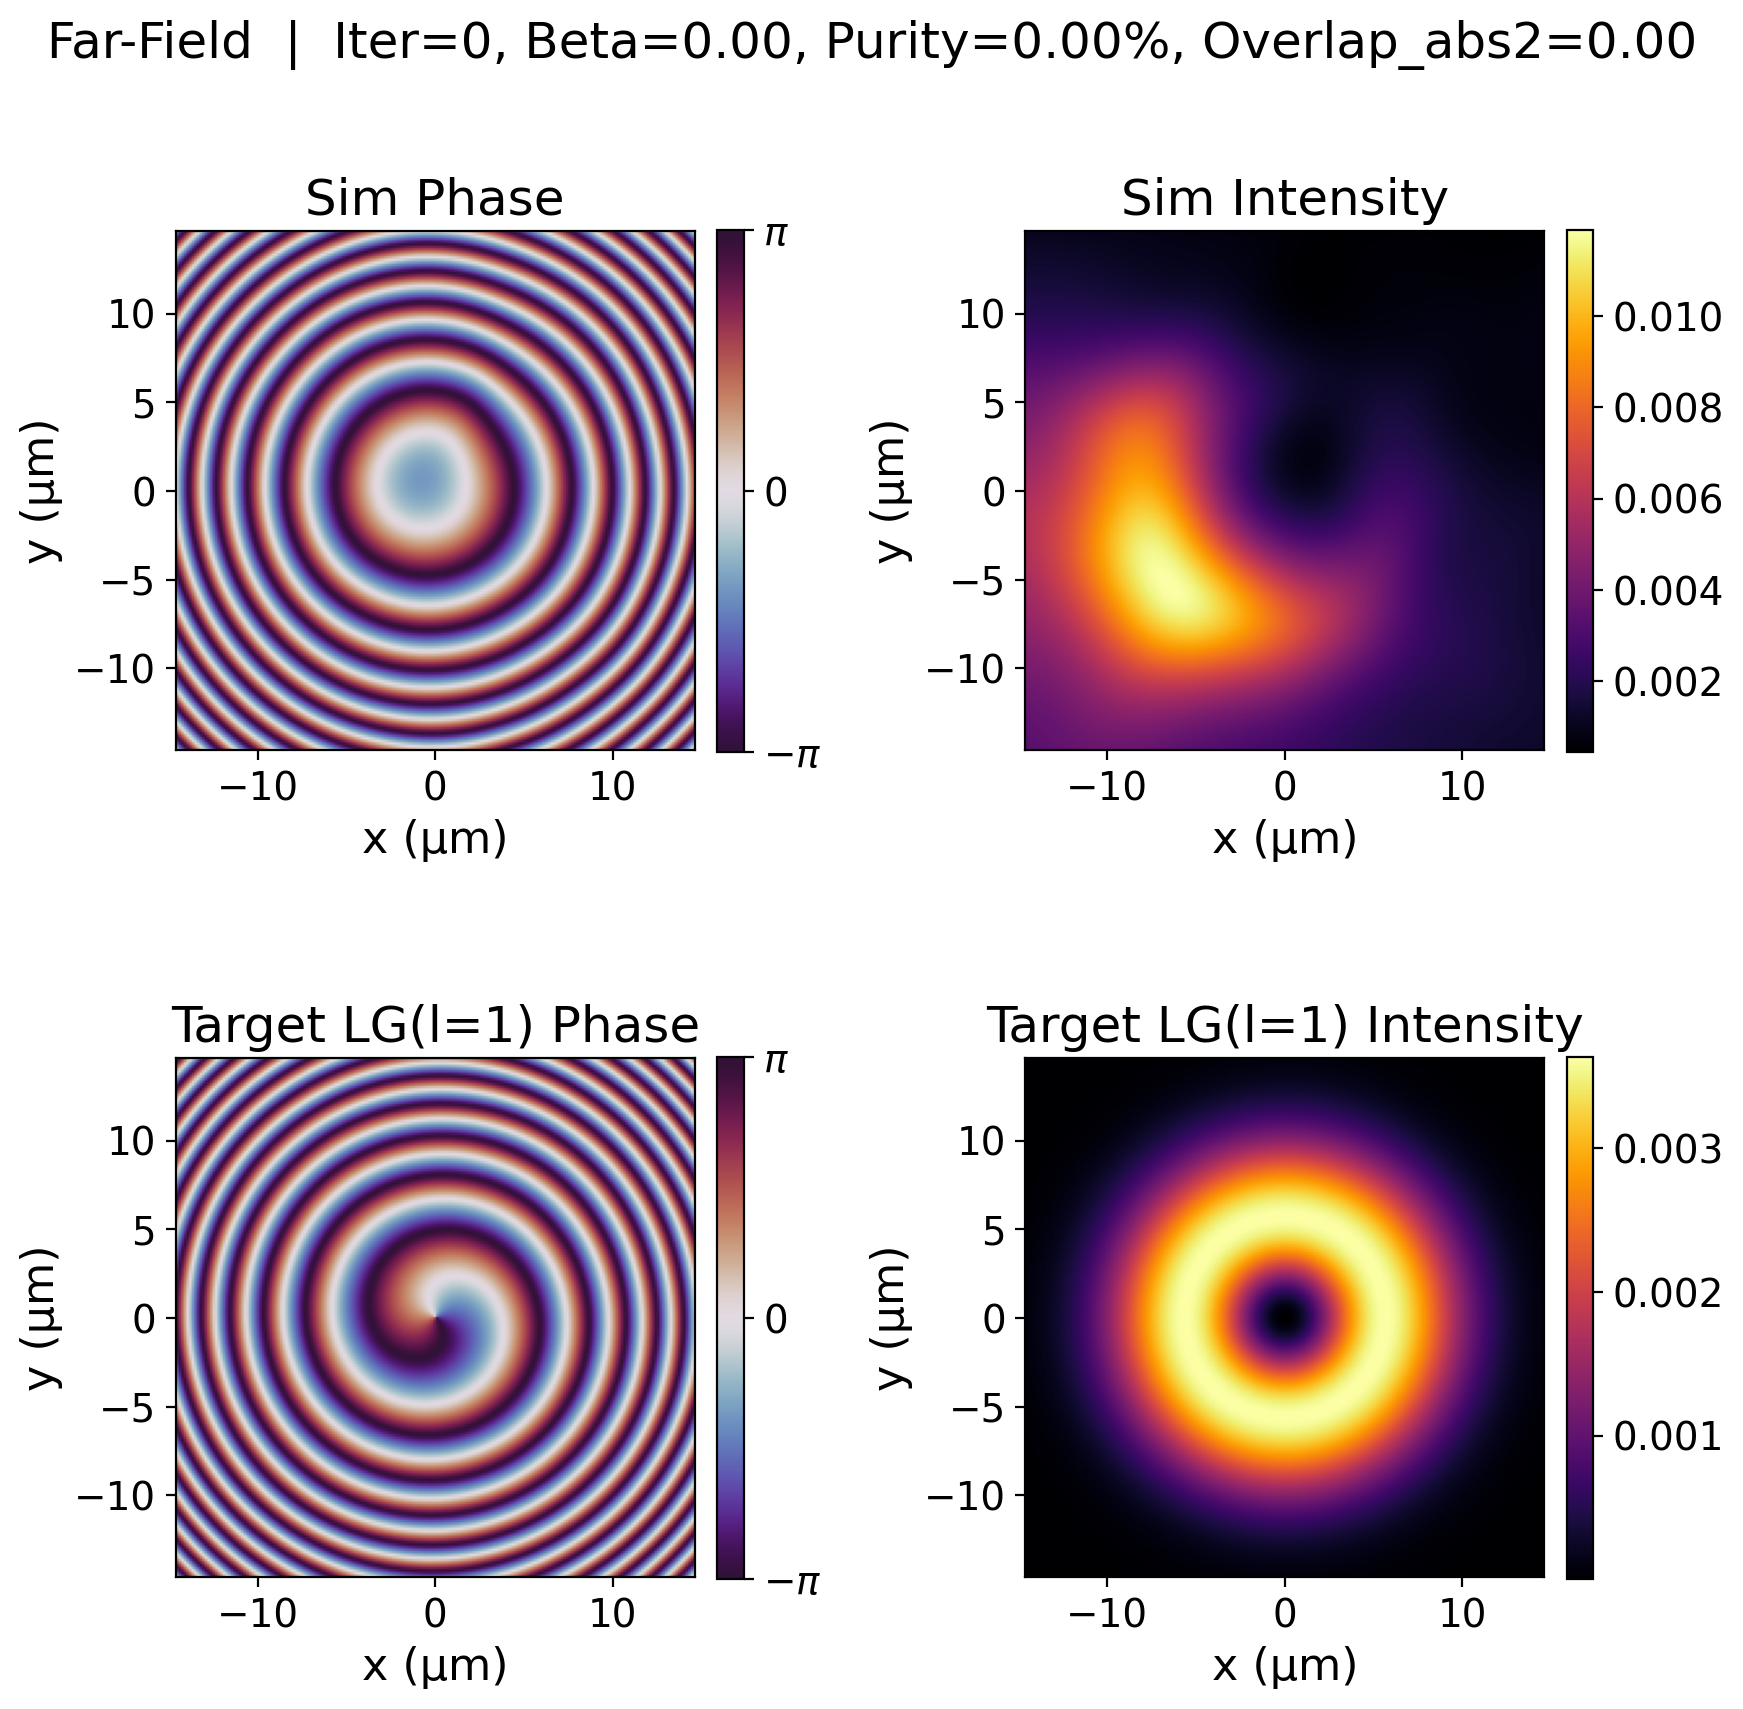
\includegraphics[width=0.30\textwidth,keepaspectratio]{img/018_ff_iter_000_beta_0.00.png} &
        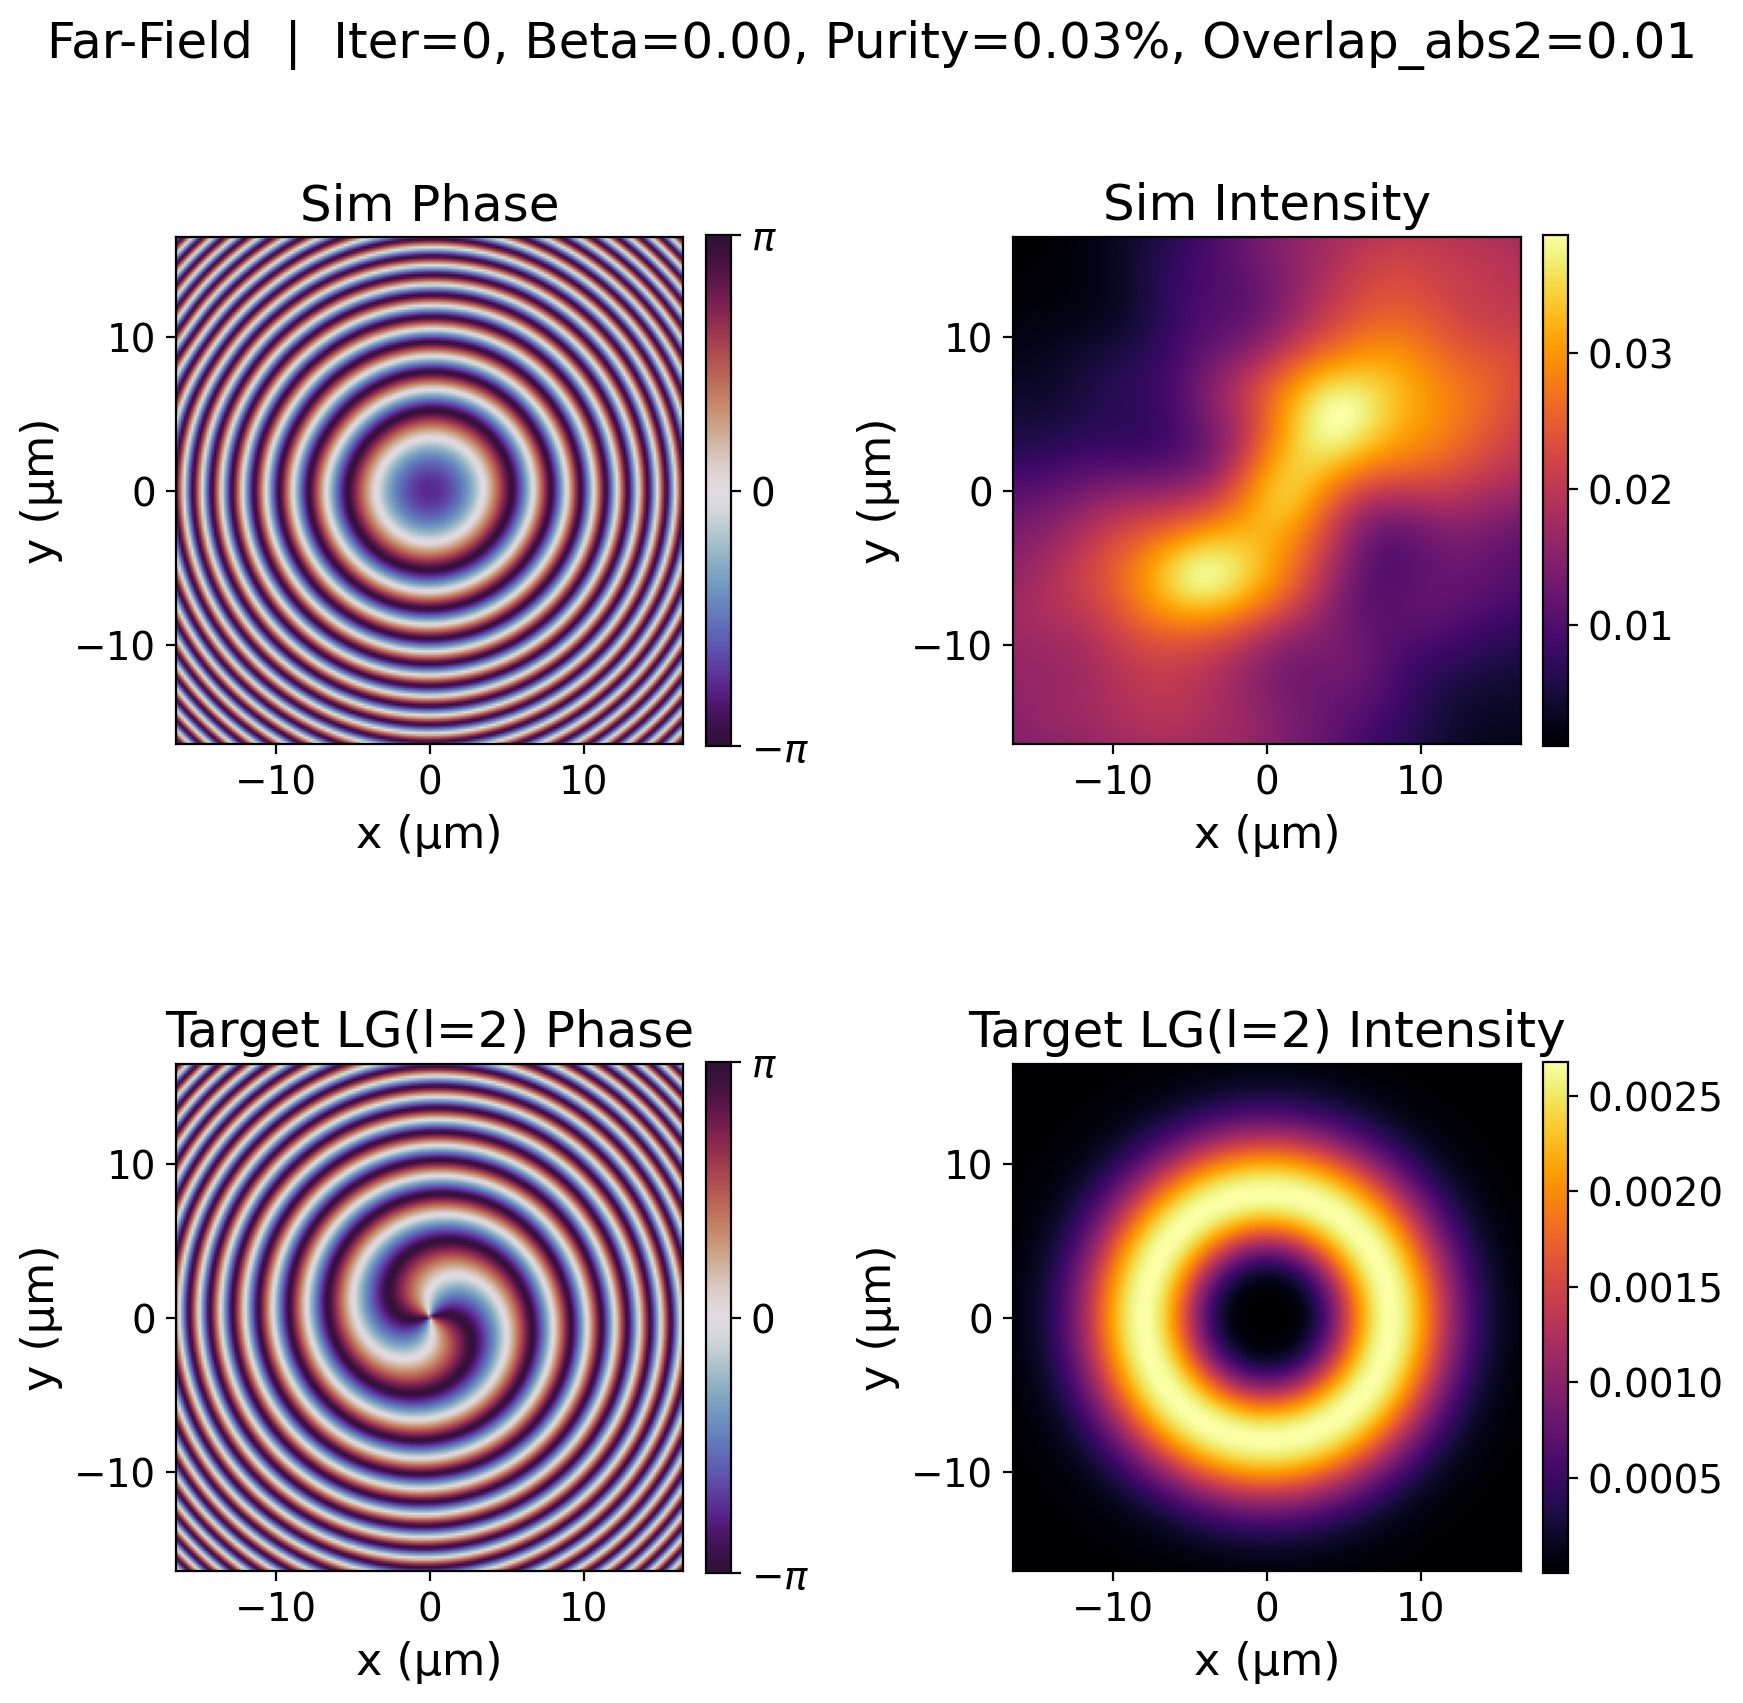
\includegraphics[width=0.30\textwidth,keepaspectratio]{img/013_ff_iter_000_beta_0.00.png} &
        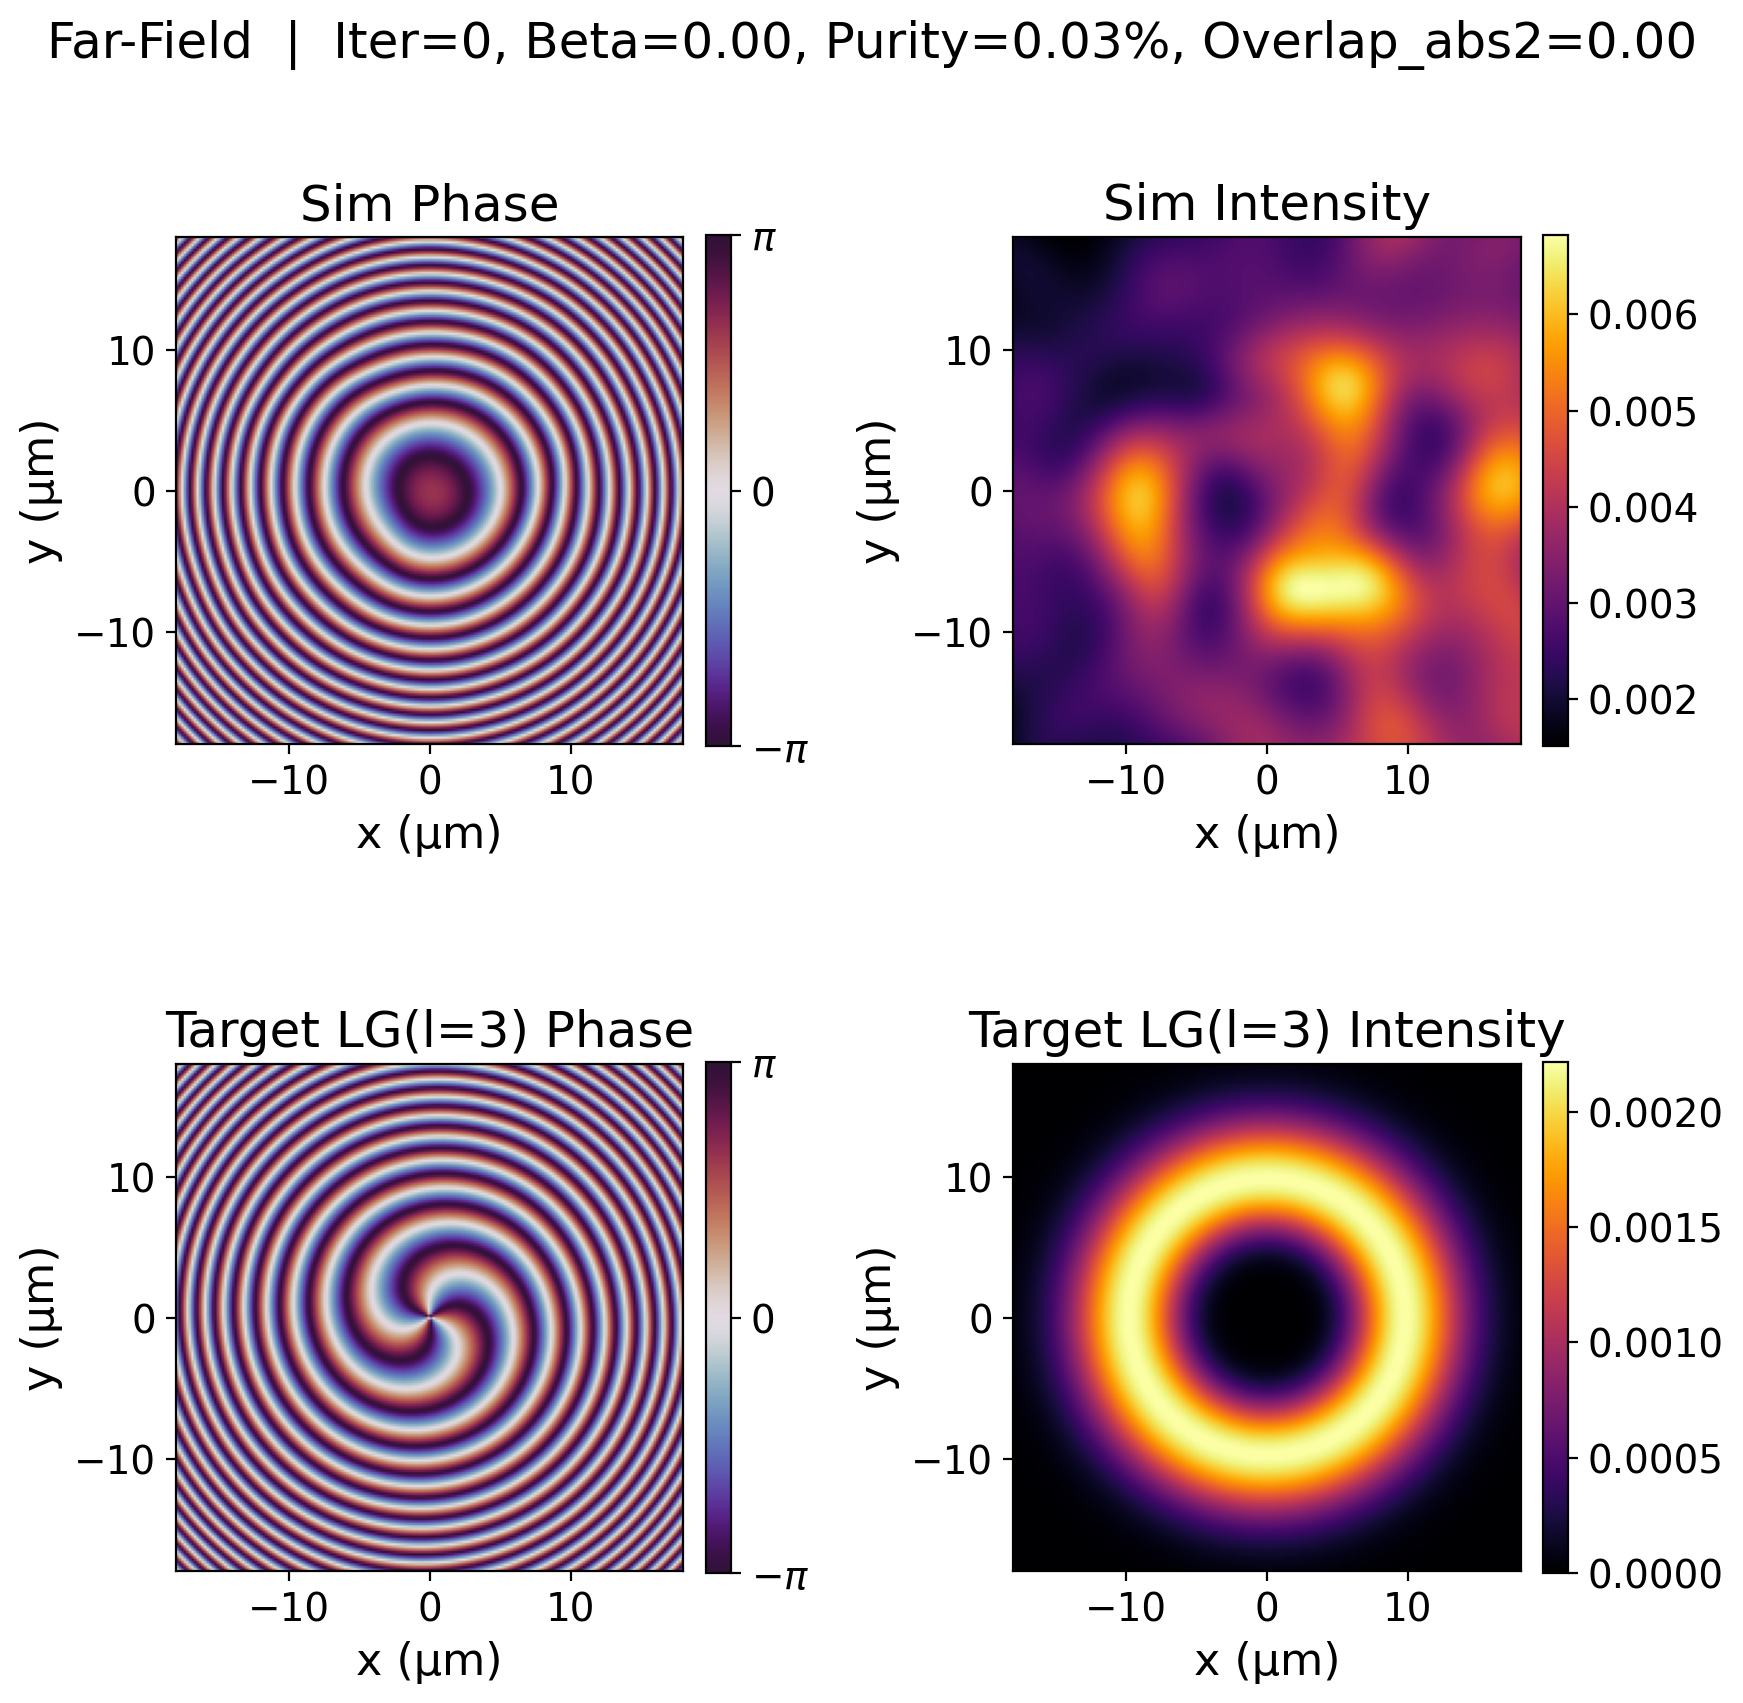
\includegraphics[width=0.30\textwidth,keepaspectratio]{img/rcp.png}
        \\ (a) $\ell=1$, RCP & (b) $\ell=2$, RCP & (c) $\ell=3$, RCP \\[8pt]
        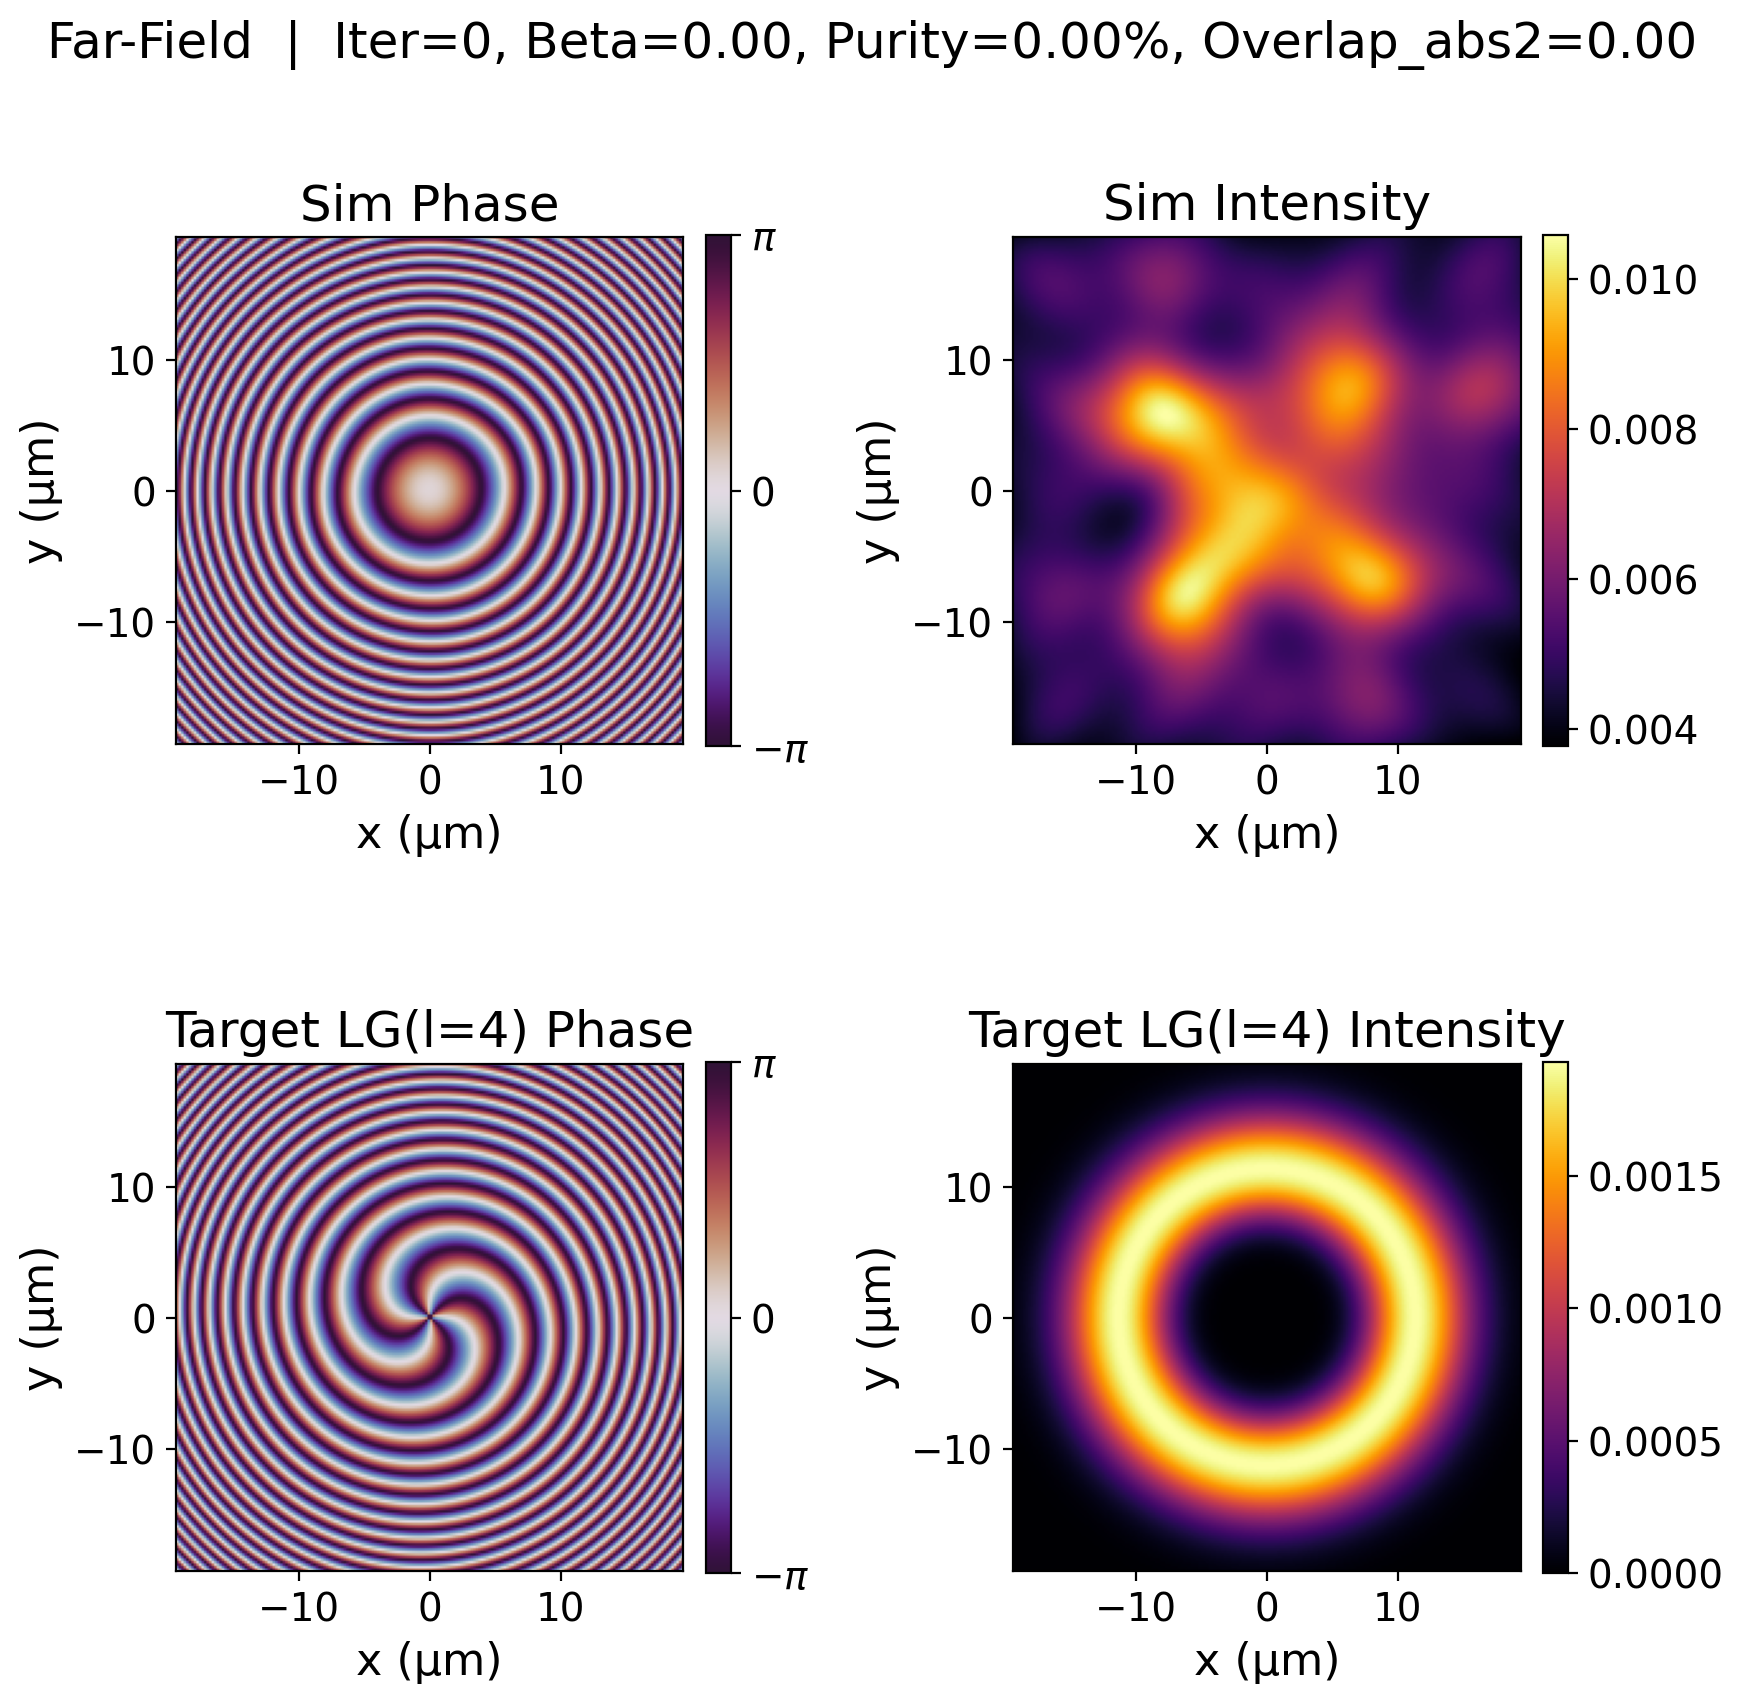
\includegraphics[width=0.30\textwidth,keepaspectratio]{img/021_ff_iter_000_beta_0.00.png} &
        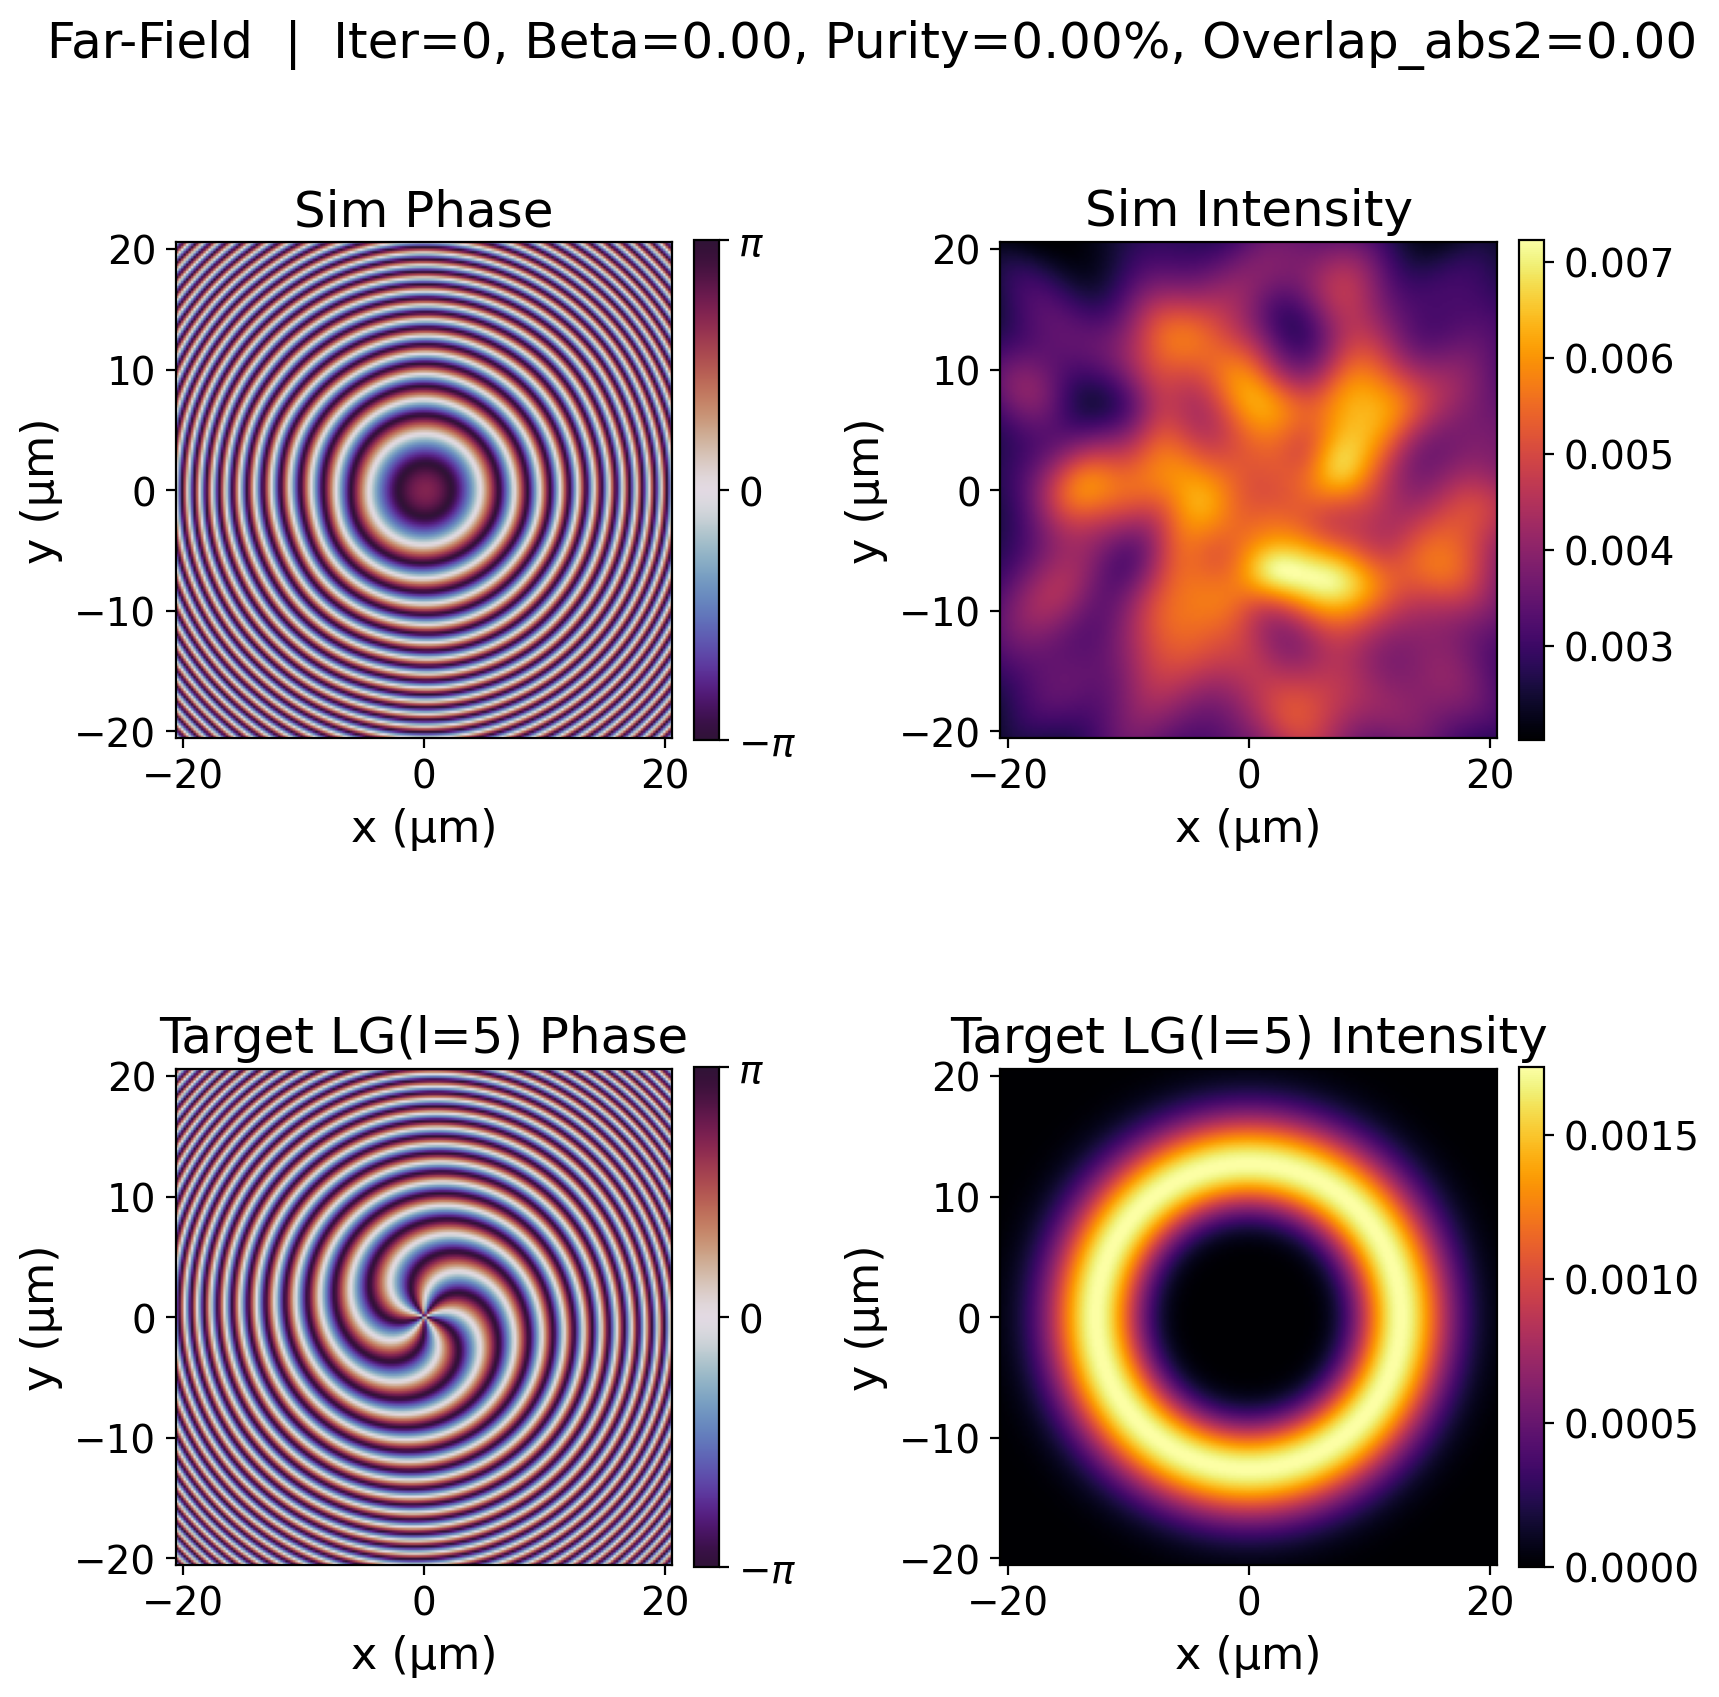
\includegraphics[width=0.30\textwidth,keepaspectratio]{img/022_ff_iter_000_beta_0.00.png} &
        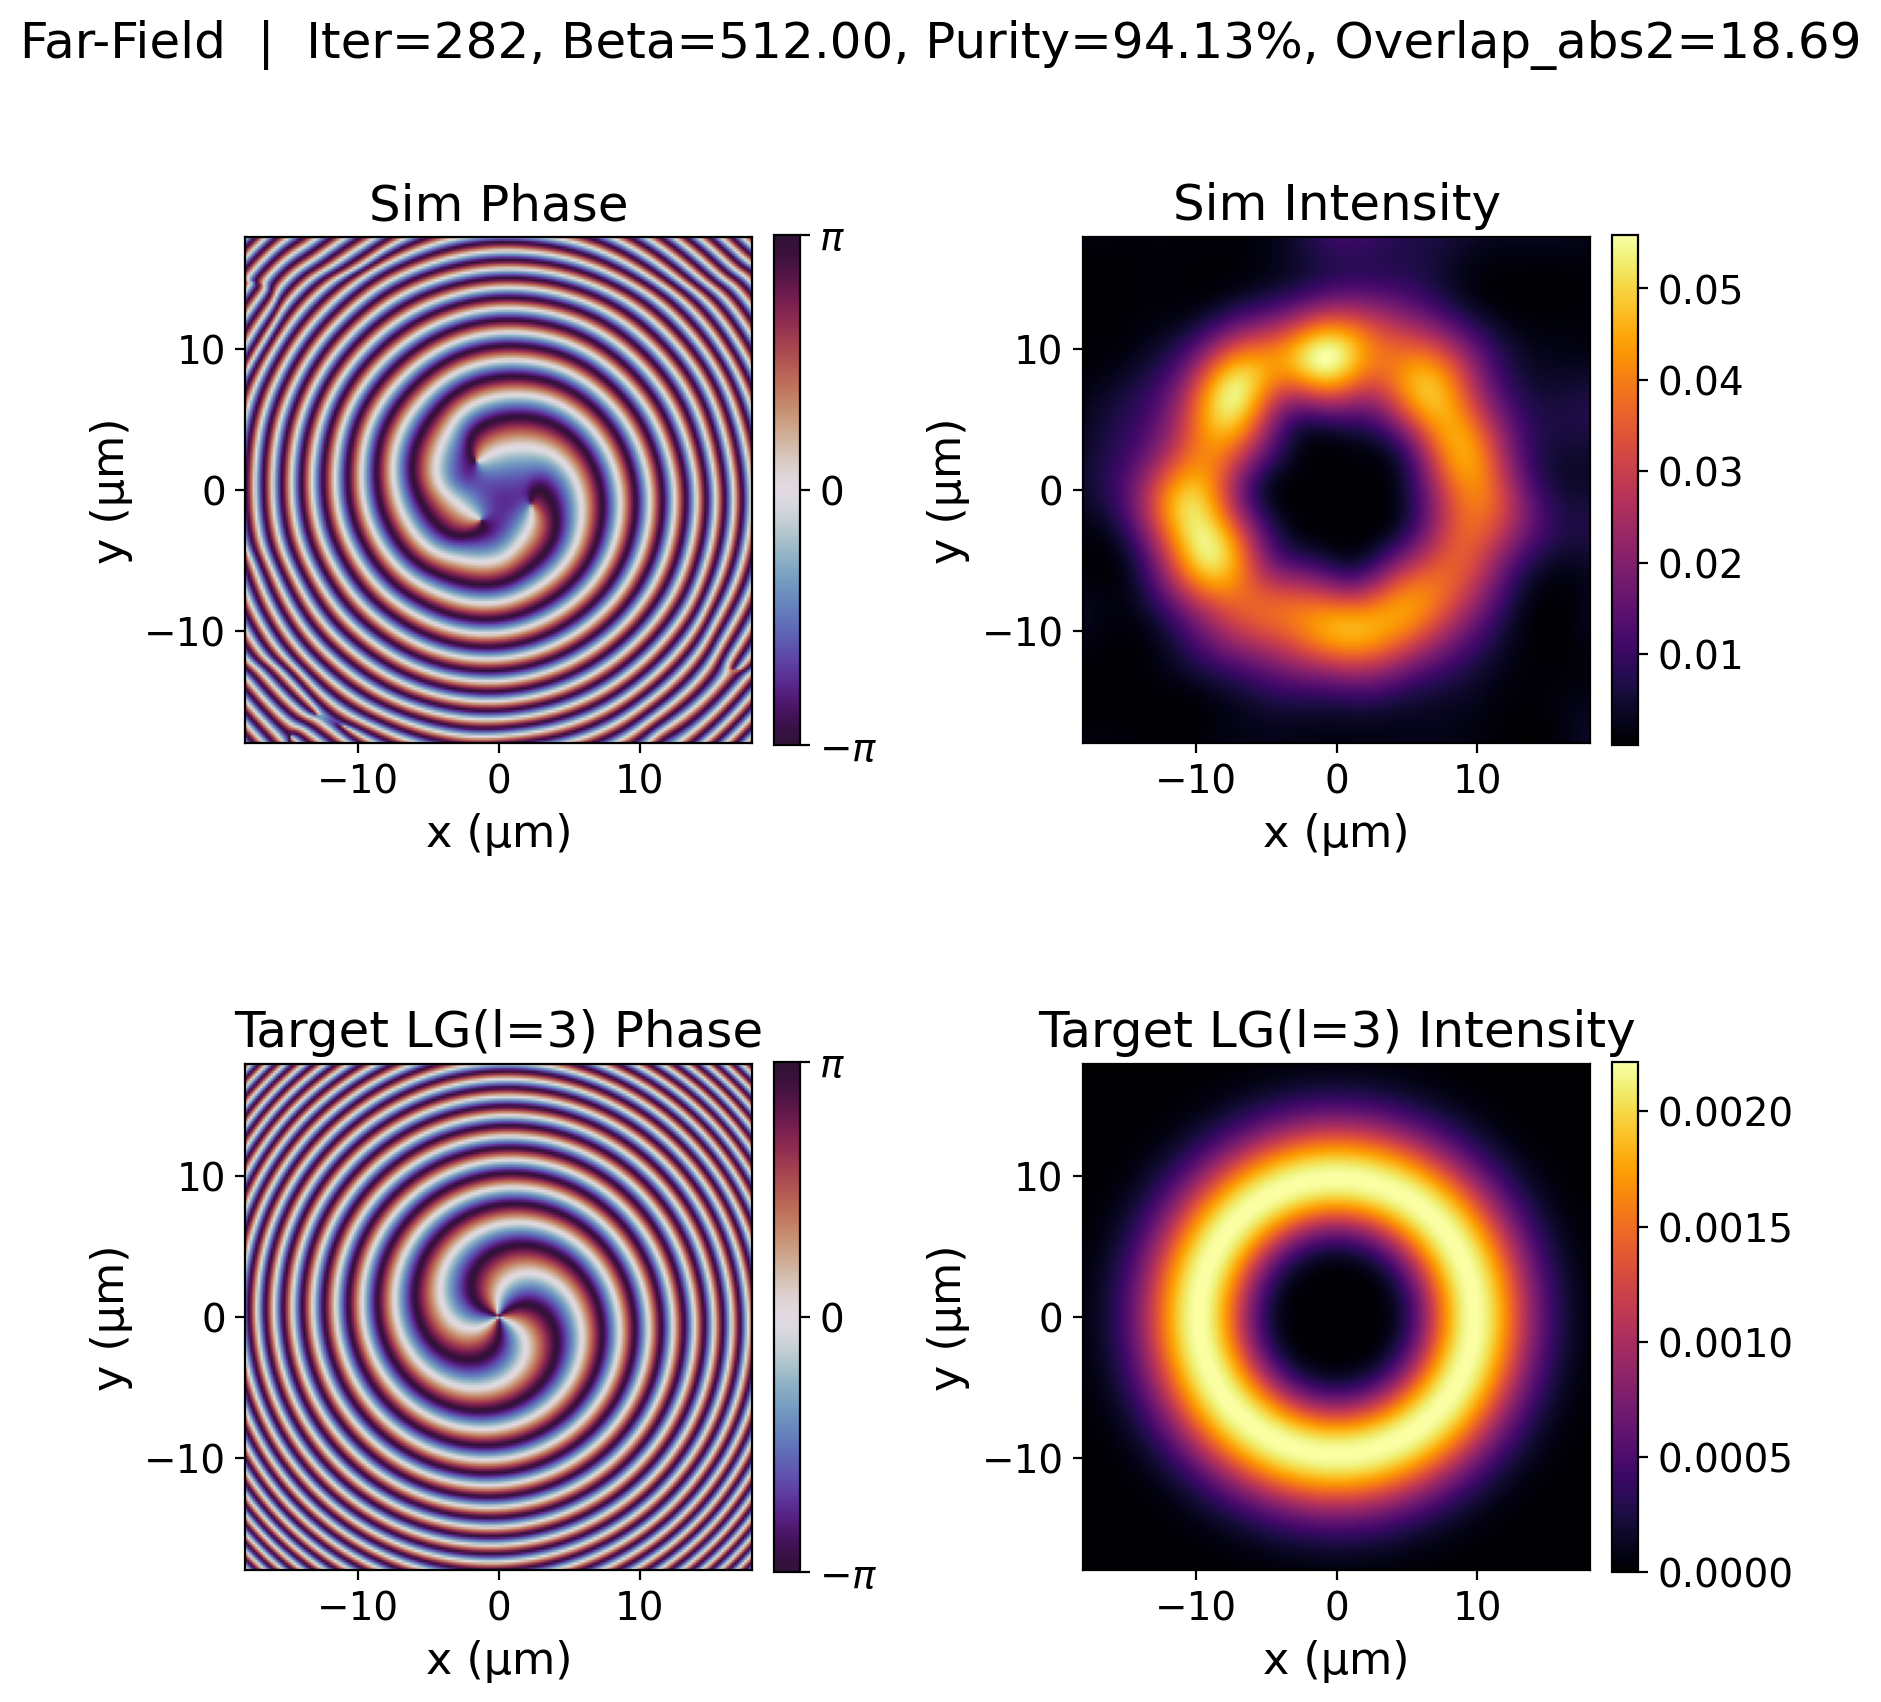
\includegraphics[width=0.30\textwidth,keepaspectratio]{img/020_ff_iter_282_beta_512.00.png}
        \\ (d) $\ell=4$, RCP & (e) $\ell=5$, RCP & (f) $\ell=3$, LCP (reference)
    \end{tabular}
\caption{Far-field OAM mode analysis under RCP cross-polarization excitation for $\ell = 1$ to $5$ ((a)--(e)), with the LCP-excited $\ell = 3$ result shown as a reference (f). Under RCP excitation, the far-field purity of the target LG mode collapses to near-zero in all cases (see Table~\ref{tab:rcp_selectivity}), and neither the characteristic doughnut intensity ring nor the spiral phase pattern is recovered, confirming very strong circular polarization selectivity for all designs.}
\label{fig:ff_purity_rcp}
\end{figure}



%===================================================================


\section{Device Energy Efficiency}
\label{sec:device_efficiency}

Beyond modal purity and phase accuracy, understanding how efficiently the source power is directed upward into the far-field collection cone is essential for assessing the device's practical utility. This section evaluates three complementary efficiency metrics for all six designs and a bare reference case:

\begin{itemize}
    \item $X$ Upward fraction): $X = P_\text{up}/P_\text{total}$, where $P_\text{up}$ is the power collected by a monitor placed above the design layer and $P_\text{total}$ is the total power radiated by the source. This metric directly quantifies the fraction of source energy redirected upward toward the far-field observation side.
    \item $Y$ (Far-field LG purity): The modal purity evaluated at $z = 10\,z_R$ (see Table~\ref{tab:results_summary}).
    \item $Z$ (Device efficiency): $Z = X \times Y$, combining upward extraction and mode quality into a single end-to-end figure of merit.
\end{itemize}

Table~\ref{tab:device_efficiency} summarizes the results for all six designs alongside a pure-air baseline (the same dipole source without any GaP nanostructure, only the diamond substrate). Figure~\ref{fig:monitor_positions} illustrates the power monitor placement.

\begin{table}[htb]
\centering
\caption{Device energy efficiency for all six optimized designs and a pure-air baseline.}
\label{tab:device_efficiency}
\begin{tabular}{cccccc}
\hline
Structure & $P_\text{up}$ (a.u.) & $P_\text{total}$ (a.u.) & $X$ (\%) & $Y$ (\%) & $Z$ (\%) \\
\hline
Pure Air (baseline) & $5.0\times10^{1}$ & $1.0\times10^{3}$ & 5.04  & 100.00 & 5.04  \\
$\ell = 0$ & $1.6\times10^{2}$ & $9.2\times10^{2}$ & 17.67 & 96.81  & 17.11 \\
$\ell = 1$ & $9.2\times10^{1}$ & $9.5\times10^{2}$ &  9.67 & 98.66  &  9.54 \\
$\ell = 2$ & $3.5\times10^{1}$ & $1.2\times10^{3}$ &  2.93 & 97.96  &  2.87 \\
$\ell = 3$ & $6.3\times10^{1}$ & $1.5\times10^{3}$ &  4.22 & 94.13  &  3.97 \\
$\ell = 4$ & $3.5\times10^{1}$ & $1.2\times10^{3}$ &  2.93 & 81.94  &  2.40 \\
$\ell = 5$ & $2.4\times10^{1}$ & $1.1\times10^{3}$ &  2.14 & 82.62  &  1.77 \\
\hline
\end{tabular}
\end{table}

The results reveal a clear performance hierarchy. The $\ell = 0$ design achieves the highest device efficiency of $Z = 17.11\%$, representing a $3.4\times$ improvement over the pure-air baseline ($5.04\%$), confirming that the Gaussian-mode nanostructure is highly effective at redirecting near-isotropic dipole radiation upward. The $\ell = 1$ design follows at $Z = 9.54\%$. Higher-order designs ($\ell \ge 2$) show significantly lower upward fractions ($X \le 4.22\%$), bringing the overall device efficiency below $4\%$ despite their high LG modal purity ($Y \ge 82\%$).

Importantly, the dominant bottleneck is the upward fraction $X$ rather than modal purity $Y$: while $Y \ge 82\%$ for all six designs, $X$ spans a much wider range from $2.14\%$ to $17.67\%$. This indicates that the optimizer successfully shapes the correct LG mode profile, but a large fraction of the emitted power is directed downward into the diamond substrate ($n = 2.40$) or scattered laterally. Improving the upward extraction efficiency---for example by introducing a metal reflector below the diamond substrate (discussed in Section~\ref{sec:future_work})---is therefore the most impactful direction for future efficiency gains.

\begin{figure}[htb]
\centering
	\begin{tabular}{cc} 
		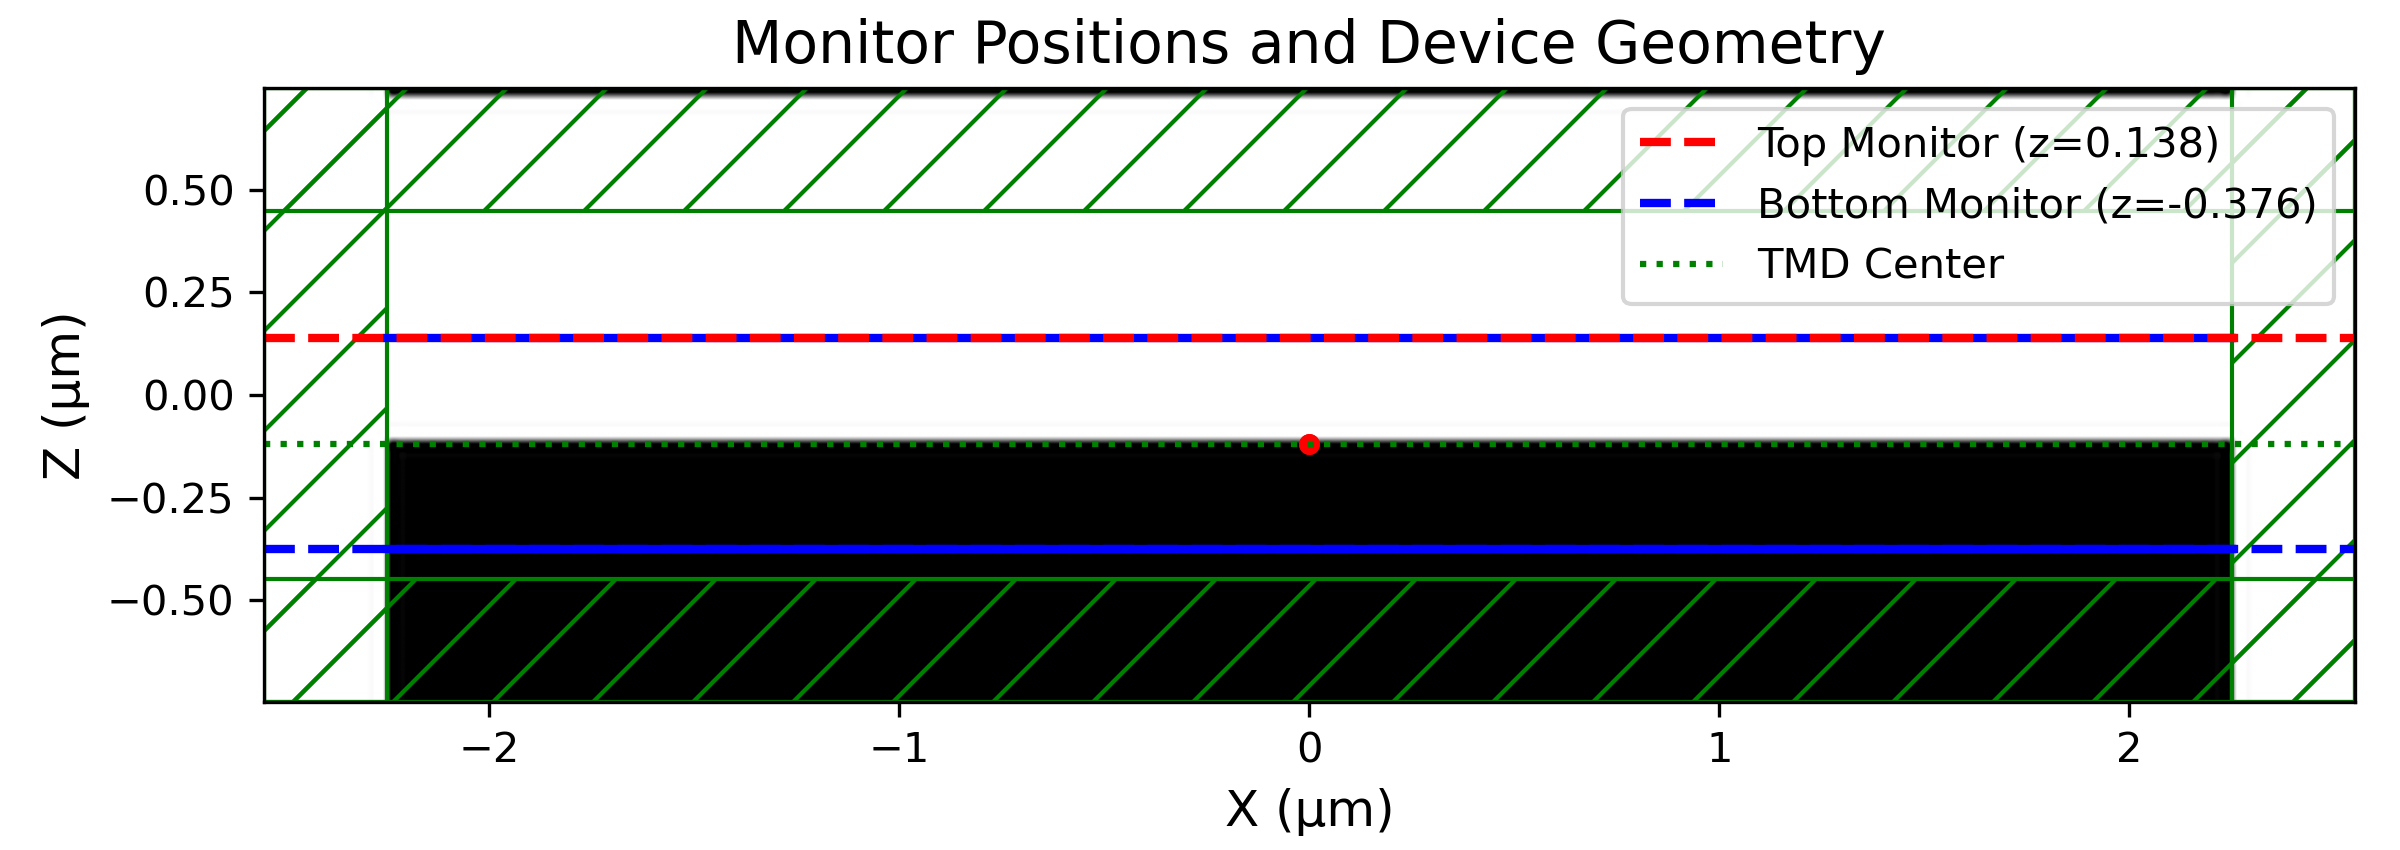
\includegraphics[width=0.48\textwidth]{img/monitor_positions_air.png} & 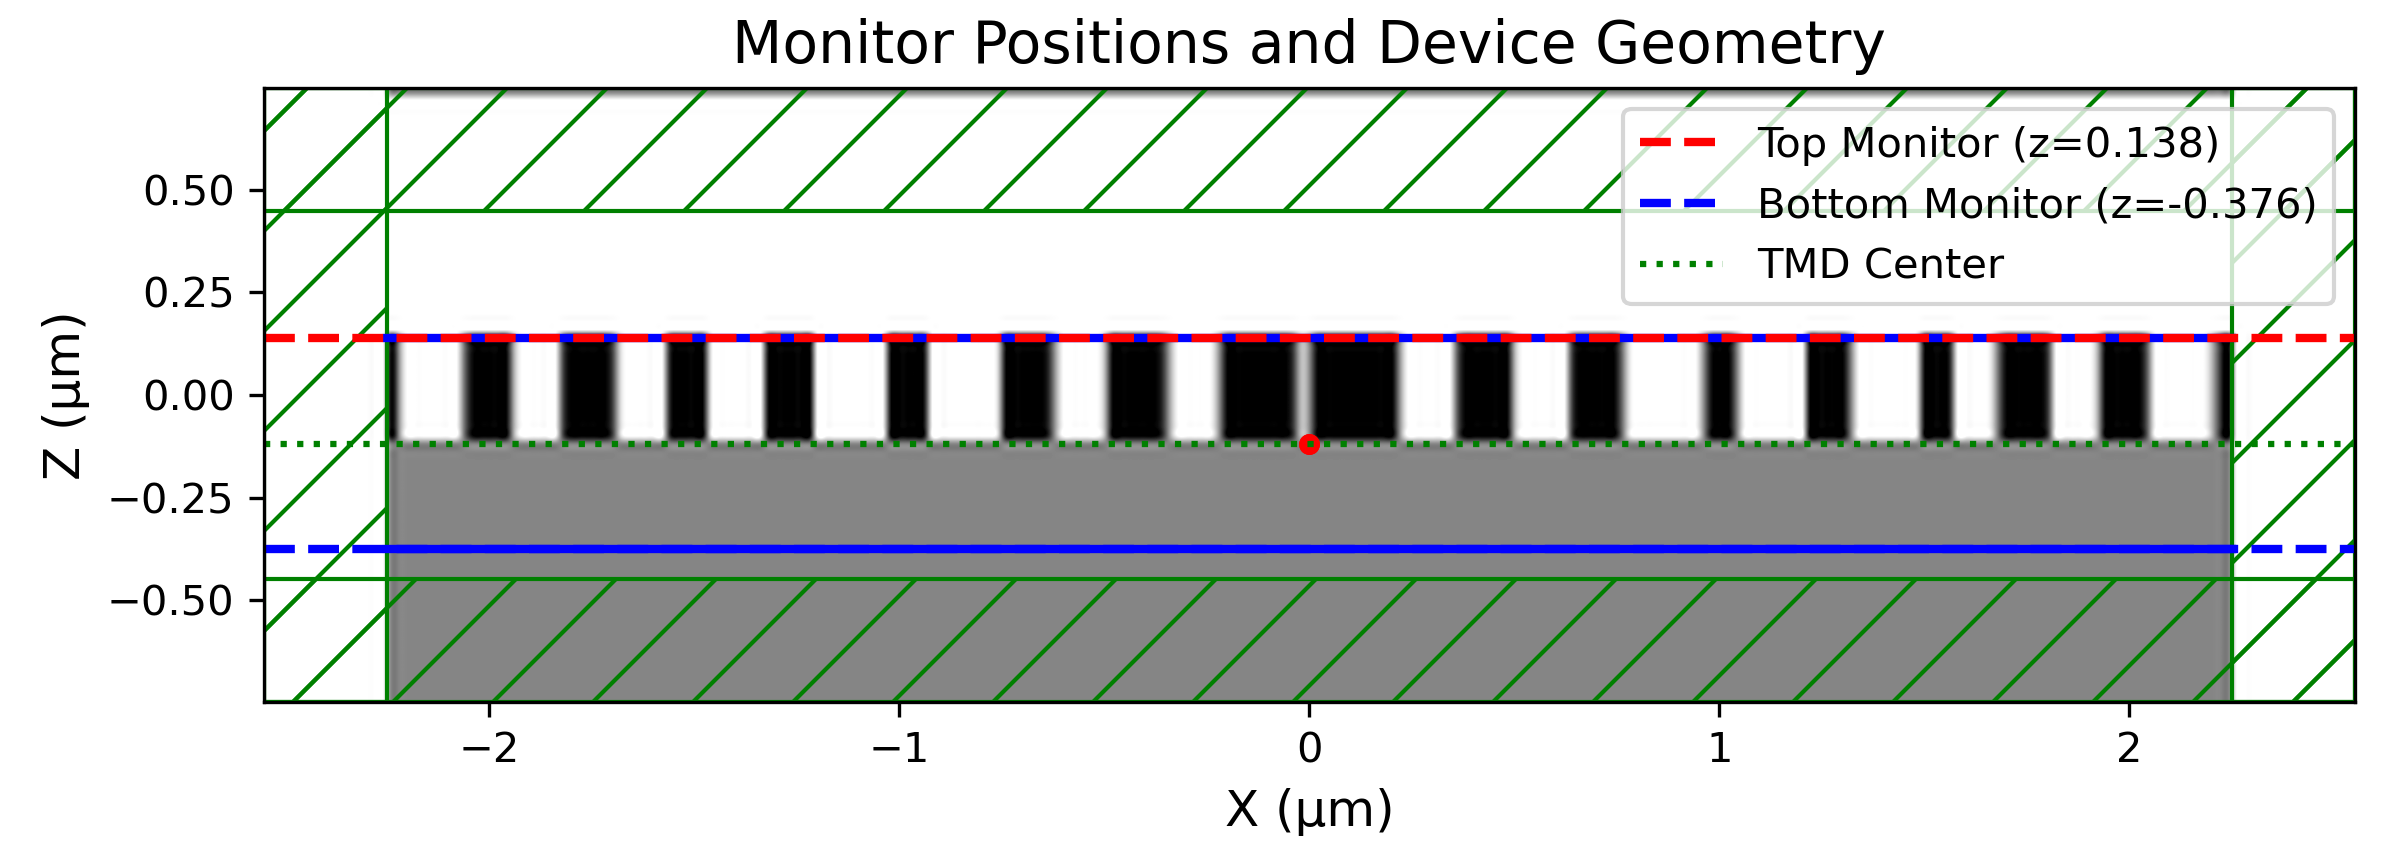
\includegraphics[width=0.48\textwidth]{img/monitor_positions_ell2.png}
		\\(a) Pure-air baseline (no GaP structure) & (b) Representative $\ell = 2$ optimized structure [6pt]
	\end{tabular}
\caption{Power monitor configuration used to evaluate upward extraction efficiency $X$. The upward monitor (red dashed line, above the design layer) captures $P_\text{up}$, while the downward monitor (blue dashed line, below the design layer) captures $P_\text{down}$, with the total power given by $P_\text{total} = P_\text{up} + P_\text{down}$.}
\label{fig:monitor_positions}
\end{figure} \newpage
\chapter{Discussion}

\label{ch:Discussion}

This chapter builds on the numerical results from Chapter 4 and explores three aspects in depth:
 (i) the physical origins of design performance and its dependence on topological charge;
 (ii) comparison and positioning relative to existing literature;
 (iii) the limitations of this work's methodology and directions for future research.

%===================================================================

\section{Physics of Topology-Dependent Performance}

\label{sec:physics_discussion}

\subsection{Mechanism of SPP-like Geometry Emergence in $\ell=2$ and Free-Form Optimization in Other Modes}

\label{ssec:spiral_emergence}

Chapter 4 showed that, for the $\ell = 2$ design, topology optimization guided by adjoint gradients spontaneously discovers a clear two-arm spiral structure at the center (Figure~\ref{fig:structures_all}(c)). This outcome has a clear physical origin: the azimuthal phase dependence $e^{i2\phi}$ of the LG$_{2,0}$ mode requires the structure to provide a continuously increasing $2 \times 2\pi$ phase difference across $\phi \in [0, 2\pi)$. This requirement is directly met by a two-arm spiral material distribution, which closely mirrors the working principle of a spiral phase plate (SPP). The surrounding scattering features act as a compensation mechanism by which the optimizer corrects near-field coupling errors, further improving the accuracy of far-field mode shaping.

For the other designs ($\ell = 0, 1, 3, 4, 5$), topology optimization does not produce simple $\ell$-fold spiral patterns. Instead, the optimizer converges to free-form, non-intuitive material distributions with no obvious geometric regularity. This reflects the nature of global topology optimization: an SPP-like spiral strategy is not always the globally optimal solution. When the spiral approach does not maximize the figure of merit, the optimizer automatically explores other structural forms. In all designs, the surrounding scattering features become denser as topological charge increases, reflecting the higher modulation demand on azimuthal phase space for higher-order OAM modes.


\subsection{Origin of the Purity--Overlap Decoupling}

\label{ssec:purity_overlap}

Table~\ref{tab:results_summary} reveals a phenomenon worth examining in depth: the Purity for $\ell = 1$ is the highest of all six ($98.66\%$), yet $|{\rm Overlap}|^2$ has already dropped from $60.92$ at $\ell=0$ to $53.88$; for $\ell = 2$, Purity is still $97.96\%$, but $|{\rm Overlap}|^2$ drops further to $7.99$. This "high purity, low overlap" phenomenon arises from the fundamentally different physical meanings of the two metrics:

Purity measures the normalized shape agreement between the far-field pattern and the target LG mode (see equation (3.9)) and is insensitive to the absolute energy level; $|{\rm Overlap}|^2$ quantifies the absolute coupling power, directly reflecting how much of the source radiation is effectively converted into the target mode. As topological charge increases, the ring peak radius of the LG$_{\ell,0}$ mode, $r_{\rm peak} = w_0\sqrt{\ell/2}$, grows rapidly, while the design region size is fixed at $4.5\,\mu{\rm m}$. Effective pattern shaping for high-$\ell$ modes can only happen within this constrained space. The optimizer can produce the correct spiral phase distribution within the finite space (maintaining high Purity), but cannot simultaneously ensure sufficient absolute energy coupling into the larger-scale modes (hence $|{\rm Overlap}|^2$ drops significantly).

This decoupling confirms that using both Purity and $|{\rm Overlap}|^2$ as dual evaluation metrics is necessary: the two are complementary—the former reflects the fidelity of the mode shape, the latter reflects the efficiency of energy conversion, and neither alone is sufficient.

\subsection{Physical Limits of High-Order OAM Generation}

\label{ssec:high_order_limit}

The mode purity for $\ell = 4, 5$ drops to around $82\%$, and slight non-uniformity appears in the far-field phase distribution (see Section~\ref{sec:farfield}). This performance drop can be attributed to two mutually coupled physical limitations:

\textbf{(i) Azimuthal phase gradient resolution limit:} High-order OAM modes require finer azimuthal phase gradients across the design region, with an equivalent azimuthal spatial frequency proportional to $\ell$. At a fixed $4.5\,\mu{\rm m}$ design area and $50\,{\rm grid/}\mu{\rm m}$ resolution, the azimuthal phase modulation needed for high topological charges gradually approaches the spatial frequency ceiling resolvable by the grid, creating a numerical bandwidth limitation—the optimizer can no longer accurately express the required fine geometric phase distribution.

\textbf{(ii) Insufficient design domain size relative to mode scale:} The ring peak radius of LG modes grows proportionally with topological charge, and for $\ell = 4, 5$ the theoretical spot size is approaching the design domain boundary. The optimizer cannot fully express the complete radiation pattern required for high-order modes within the finite design space, limiting far-field mode shaping.

These two limitations together form the performance bottleneck of this work at high $\ell$, and suggest that expanding the design region or increasing numerical resolution would likely significantly improve mode purity for high-order modes. Notably, despite these spatial constraints, the phase winding verification for all designs (Section~\ref{sec:winding}) shows topological charge accuracy errors below $1\%$, indicating that the performance loss at high $\ell$ is primarily expressed as deviations in the intensity profile, not as misalignment of the topological charge itself.

  

%===================================================================

\section{Comparison with Prior Work}

\label{sec:comparison}

\subsection{Metasurface-Based OAM Emitters}

\label{ssec:compare_metasurface}

\begin{table}[htb]
\centering
\caption{Quantitative comparison of this work with representative existing OAM metasurface approaches.}
\label{tab:comparison}
\resizebox{\textwidth}{!}{%
%\begin{tabular}{p{2.8cm}cccp{2.5cm}c}
\begin{tabular}{cccccc}
\hline
Approach & Design method & Material & Purity (\%) & Source type & Valley selectivity \\
\hline
Karimi 2014 \cite{karimi2014generating} & Forward (geometric phase) & Au plasmonic & $\sim$64 & External plane wave & None \\
Guo 2016 \cite{guo2016merging} & Forward (geometric+propagation phase) & Au plasmonic & $>$90 & External plane wave & None \\
Sroor 2020 \cite{sroor2020high} & Forward ($\text{TiO}_2$ metasurface) & $\text{TiO}_2$ all-dielectric & $\sim$90  ($\ell \le 100$) & Intracavity laser & None \\
Li 2023 \cite{li2023valley} & TMD photonic crystal (BIC) & $\text{WSe}_2$/Si & Purity not quantified & \textbf{Active ($\text{WSe}_2$)} & Fixed $\ell$ \\
\textbf{This work} & \textbf{Inverse design (topology optimization)} & \textbf{GaP all-dielectric} & \textbf{82$\sim$ 98 ($\ell \le 3$)} & \textbf{Active ($\text{WS}_2$)} & \textbf{Fixed $\ell$ \& RCP purity $<1\%$} \\
\hline
\end{tabular}
}
\end{table}


Table~\ref{tab:comparison} summarizes a quantitative comparison of this work with representative literature on core metrics. As can be seen, this work holds clear advantages over existing approaches in three dimensions:

\textbf{(i) Simultaneous high purity and active chiral source integration:} Existing approaches either achieve high purity (Sroor 2020: $\sim 90\%$) but use an intracavity metasurface laser, which is a large laser setup rather than emitter integration, and lacks valley selectivity; or combine TMD material  with metasurfaces to act as an active circularly polarized light source (Li 2023) but do not quantify LG mode purity and are limited by fixed lattice geometry. This work achieves LG mode purity ranging from $98.66\%$ ($\ell = 1$) to $94.13\%$ ($\ell = 3$), while simultaneously integrating an active valley-polarized exciton source, filling the "active source + high-purity LG mode" design gap.

\textbf{(ii) Quantitative verification of valley polarization selectivity:} Only a small number of existing works have quantified inter-valley crosstalk. This work directly provides a clear, experimentally benchmarkable baseline through the RCP cross-excitation test ($\ell = 3$ structure: RCP purity $0.03\%$ vs. LCP purity $94.13\%$).

\textbf{(iii) Design freedom:} Using $5.1\times10^4$ design degrees of freedom instead of the traditional few geometric parameters allows the optimizer to automatically search for non-intuitive high-performance structures without any preset geometric shape.

\textbf{(iv) Compact footprint:} The device footprint of this work is $4.5 \times 4.5\;\mu\text{m}^2$. This small size is close to the exciton diffusion length in monolayer $\text{WS}_2$, which helps to reduce intervalley scattering during emission. Topology optimization makes this compact size possible by encoding the full phase profile within a single non-periodic design region. This allows the device to achieve high OAM purity and active valley-locked emission within an ultra-compact footprint.

\subsection{Topology Optimization in Nanophotonics}

\label{ssec:compare_topo}

There are many precedents for applying topology optimization to nanophotonics, including photonic crystal cavity mode shaping and nonlinear frequency conversion efficiency optimization \cite{Hammond2022high}. However, inverse design approaches directly targeting chiral active light sources combined with OAM mode integration remain rare in the existing literature.

The main methodological contributions of this work lie in three points. First, a chiral emitting point source is used as the optimization driving field, so the resulting structure corresponds from the start to the actual radiation environment of valley-polarized excitons. Second, the joint logarithmic objective function of LG mode overlap integral and mode purity (equation (3.16)) is used as the FOM, preventing low-power pathological convergence while maintaining precise control over mode shape. Third, the circular polarization selectivity of the design is maintained throughout, and quantitatively verified through near-field chirality density analysis and polarization cross-excitation testing (Sections~\ref{sec:chirality} and \ref{sec:pol_selectivity}).

%===================================================================

\section{Limitations and Future Directions}

\label{sec:limitations}

\subsection{Current Limitations}

\label{ssec:current_limits}

This work has several limitations worth acknowledging, and their impact on the reliability of the results is assessed for each:

\textbf{(i) Fixed design region size:} The $4.5\,\mu{\rm m}$ design side length is adequate for low topological charges ($\ell \le 2$), but for $\ell = 4, 5$ the theoretical LG spot peak radius $r_{\rm peak} = w_0\sqrt{\ell/2}$ is approaching or exceeding the design domain boundary, and the optimizer cannot fully express the radiation pattern of high-order modes within the finite space (see Section~\ref{ssec:high_order_limit} for details). Based on estimates, expanding the design domain to $6.5\,\mu{\rm m}$ or more could restore the mode purity for $\ell = 4, 5$ to above $85\%$.

\textbf{(ii) Single-wavelength design:} This work optimizes at a single target wavelength $\lambda = 0.593\,\mu{\rm m}$ (near the WS$_2$ exciton peak wavelength). GaP has relatively small dispersion near this wavelength ($\Delta n/\Delta\lambda \approx 0.3\,\mu{\rm m}^{-1}$), and purity is expected to remain above $80\%$ within about $\pm 5\%$ of the target wavelength, but this requires further simulation verification. For practical applications involving multi-wavelength OAM multiplexing, the FOM definition would need to be extended with multi-band constraints, or a broadband optimization strategy would need to be adopted.

\textbf{(iii) Ideal dipole source approximation:} The numerical model simulates WS$_2$ exciton radiation as an ideal circularly polarized point dipole ($100\%$ circular polarization purity), without accounting for three practical factors: (a) non-monochromaticity from exciton linewidth ($\sim$ tens of meV); (b) depolarization from inter-valley scattering at room temperature (experimental room-temperature valley polarization degree is typically $20\text{--}50\%$); (c) multi-exciton superposition effects. If the actual valley polarization degree $P_c$ is used as input, the far-field LG mode purity will approximately scale as ${\rm Purity}_{\rm exp} \approx P_c^2 \times {\rm Purity}_{\rm sim}$. This means that even with ${\rm Purity}_{\rm sim} = 98.66\%$, if $P_c = 50\%$, the experimentally expected purity would drop to about $25\%$; if Purcell enhancement raises $P_c \to 80\%$, it could recover to $\sim 63\%$. Improving the excitonic valley polarization purity is critical for actual device performance.

\textbf{(iv) Binary material assumption and fabrication tolerance:} The final structure is an ideally binarized GaP/air distribution. In actual fabrication, sidewall roughness ($\sim 5\,{\rm nm}$), etch depth errors ($\pm 5\%$), and GaP film refractive index non-uniformity could all introduce additional phase noise. Fabrication tolerance analysis should be an important part of future work, to establish a reliable mapping from numerical prediction to experimental measurement. Improvement directions for all of the above limitations will be proposed in Chapter 6. \newpage
\chapter{Conclusions}
\label{ch:conclusion}

%===================================================================

\section{Summary of Findings}
\label{sec:summary}

本研究建立了一套基於拓樸最佳化的全介電質奈米結構反向設計平台，
以單層 WS$_2$ 谷極化激子為主動手性光源，
系統性地設計並驗證了可將圓偏振點光源轉化為高純度拉格耳–高斯（LG）渦旋光束的奈米結構，
目標模態涵蓋 LG$_{\ell,0}$，$\ell = 0$ 至 $\ell = 5$。主要結果彙整如下：

\begin{enumerate}

    \item \textbf{高純度 OAM 模態生成：}
    在 $\ell \le 3$ 的範圍內，最佳化結構的遠場 LG 模態純度均超過 $94\%$，
    其中 $\ell = 1$ 達六組最高的 $98.66\%$；
    $\ell = 4, 5$ 受限於有限設計空間（$4.5\,\mu$m），模態純度約為 $82\%$。
    所有六組設計的相位纏繞驗證誤差均低於 $1\%$，
    精確確認遠場渦旋光束攜帶正確的目標拓樸荷。

    \item \textbf{螺旋對稱幾何自發湧現：}
    最佳化結構在伴隨法梯度引導下自發形成 $\ell$ 重螺旋對稱幾何，
    物理上對應 LG$_{\ell,0}$ 模態所需的連續 $\ell \times 2\pi$ 相位分佈，
    並在外圍疊加散射補償特徵以提升模態整形精度（詳細機制分析見第~\ref{ssec:spiral_emergence} 節）。

    \item \textbf{圓偏振選擇性驗證：}
    以 $\ell = 3$ 結構進行偏振交叉激發測試：
    LCP 激發下目標模態純度 $94.13\%$；
    反向 RCP 激發下純度暴跌至 $0.84\%$（對比度 $> 100:1$），
    定量確認最佳化結構具備強烈的圓偏振篩選能力，
    能有效區分 WS$_2$ 的 K/K$'$ 雙谷。

    \item \textbf{近遠場手性演化機制釐清：}
    光學手性密度沿傳播軸分析顯示，近場因局域散射呈 LCP/RCP 混合態；
    進入遠場輻射區（$z \ge z_R$）後，漸逝波衰減，傳播場完全恢復為純淨 RCP 手性態，
    建立了從近場激發到遠場 OAM 渦旋光束的完整物理圖像（詳見第~\ref{ssec:chirality_prop} 節）。

\end{enumerate}

%===================================================================

\section{Significance and Contributions}
\label{sec:significance}

本研究的核心貢獻在於提出並驗證了一條以主動谷極化光源驅動的晶片級 OAM 發射器設計路徑。
相較於現有依賴外部平面波激發的被動超穎表面方案（如 Sroor 2020 達 $\sim 90\%$ 純度但無谷選擇性）
以及既有的谷-OAM 結合平台（如 Li 2023 具備谷選擇性但未量化 LG 模態純度），
本研究在「主動光源 + 高純度 LG 模態 + 可量化谷間對比度」三個維度上同時具備競爭優勢。

在方法學層面，本研究發展了一套整合 FDTD 電磁模擬、伴隨法梯度計算、$\beta$ 連續遞增策略與 MMA 求解器的完整拓樸最佳化流程，
並以模態純度與絕對重疊積分的聯合對數目標函數兼顧模態形狀保真度與能量耦合效率。
此框架具備高度通用性，可直接延伸至其他目標模態、光源配置或材料體系。

在物理理解層面，本研究揭示了 Purity 與 $|{\rm Overlap}|^2$ 隨拓樸荷增大的解耦機制，
闡明固定設計域尺寸下高階 OAM 整形的物理極限（詳見第~\ref{ssec:purity_overlap} 節），
為後續高階渦旋光束發射器的設計指標選取提供了重要參考。

%===================================================================

\section{Future Work}
\label{sec:future_work}

基於本研究成果，以下四個方向最具立即延伸價值：

\textbf{（一）擴大設計域與提升解析度：}
針對 $\ell \ge 4$ 的高階模態，系統性探討擴大設計面積（目標 $\ge 8\,\mu$m）與提升網格解析度對模態純度的提升效果，
以突破當前 $82\%$ 的效能瓶頸。

\textbf{（二）雙谷 OAM 多工：}
結合 WS$_2$ 的 K/K$'$ 雙谷選擇性，設計同時響應 LCP（$+\ell$）與 RCP（$-\ell$）激發的雙通道 OAM 發射器，
實現基於谷自由度的拓樸荷雙工編碼。
主要挑戰在於如何在單一結構中同時滿足兩個互相正交偏振輸入的 OAM 整形目標，
需於 FOM 中引入雙光源多目標優化框架。

\textbf{（三）製程公差分析與實驗驗證：}
以本研究最佳材料分佈作為直接設計輸入，
首先進行 FDTD 製程公差模擬（邊壁粗糙度 $\pm 5\,{\rm nm}$、蝕刻深度 $\pm 5\%$），
評估實驗預期的純度範圍，
再進行 GaP 薄膜電子束微影與反應離子刻蝕，
並以光激發 WS$_2$ 量測遠場 OAM 模態純度，
完成從數值預測到實驗驗證的完整研究閉環。

\textbf{（四）Purcell 腔增強與谷極化純度提升：}
如第~\ref{ssec:current_limits} 節所指出，實驗中 WS$_2$ 的有限谷極化純度（室溫 $20$--$50\%$）是限制實際器件性能的關鍵因素。
結合光子晶體微腔或 Fabry-Pérot 腔的 Purcell 效應，可加速激子自發輻射速率，
在競爭性去極化機制主導前完成光子提取，
有望將實驗谷極化度提升至 $>80\%$，顯著改善最終 OAM 模態純度。

 \newpage


% ====================================================
% 13. 參考文獻 Reference (檔案名稱 ref.bib)
%\ClearShipoutPicture % 把ref的浮水印關掉

\iftoggle{toc-use-cn} % 使用中文
{\addcontentsline{toc}{chapter}{參考文獻}
\renewcommand{\bibname}{參考文獻}} 
{\addcontentsline{toc}{chapter}{References}
\renewcommand{\bibname}{References}
} 


\bibliographystyle{IEEEtran}
\bibliography{ref}




% 14. 附錄 Appendix (用不到可以直接註解)
%\chapter{Appendix 附錄}
\label{ch:appendix}

本附錄整理撰寫論文時常見的排版與語法注意事項，供大家撰寫與校稿時參考，請記得看latex的語法。(此段落主要由ChatGPT撰寫整理 XD)

\section*{文字與標點}
\begin{itemize}
  \item 英文引號請使用成對反引號與直引號：``text'' → “text”。
  \item 破折號（dash）有三種：`-`（連字號，如 \textit{pre-trained}）、`--`（範圍，如 10--20）、`---`（句中強調，如 the result---as expected---was correct）。
  \item 省略號請使用 \verb|\ldots| 而非三個句點：A, B, C\ldots, Z。
  \item 數值與單位間需留不換行空白：10~km，30$^\circ$C。
  \item 中英文混排時，中文與英文之間宜留一半形空白，例如：中文 English 中文。
\end{itemize}

\section*{數學與符號}
\begin{itemize}
  \item 數學變數自動為斜體，單位或文字常數須使用 \verb|\mathrm{}| 或 \verb|\text{}|，如 $v=10~\mathrm{m/s}$。
  \item 三角函數、極值運算等應以數學命令表示：$\sin\theta$, $\max(x,y)$。
  \item 向量或矩陣可用粗體：$\mathbf{x}=[x_1,x_2]^\top$。
  \item 多行方程式請使用 \texttt{align} 環境，勿以多個 \texttt{equation} 拆寫。
\end{itemize}


\section*{圖表與引用}
\begin{itemize}
  \item 圖片標題（caption）置於圖下方
  \item 表格標題置於表上方。
  \item 參照圖表時請使用 \verb|\ref{}| 或 \verb|\autoref{}|，勿手動輸入編號。\\
        例：As shown in Fig.~\ref{fig:excel2latex}.
  \item 表格建議使用 \texttt{booktabs} 套件：\verb|\toprule|、\verb|\midrule|、\verb|\bottomrule|。
\end{itemize}

\section*{文獻與引用}
\begin{itemize}
  \item 文獻引用使用 \verb|\cite{key}| 或 \verb|\parencite{key}|。
  \item 多篇同時引用可寫為 \verb|\cite{a,b,c}| → [1–3]。
  \item 特殊大小寫（如 GPU, LaTeX）須以大括號保留：\verb|{GPU}|。
\end{itemize}
 \newpage


% =========================================
% [113年2月19日後上傳圖書館博碩士論文系統者適用] 
% 15. 學位論文發表形式確認書
% 16. 著作彙編之學位論文資訊及彙編學術著作之共同作者貢獻聲明書
% 這兩個不用附在論文PDF檔裡面

% 說明1: https://aa.nycu.edu.tw/userfiles/aach/files/20240125111443441.pdf
% 說明2: "國立陽明交通大學著作彙編之學位論文應行注意事項" https://bit.ly/457NTHk

% [心得感想]
% 畢業論文有使用到"就學期間發表"的論文, 就要填寫. 畢業後才刊登論文, 就屬於"不是".
% 對博士生來說, 在學期間可能發表很多篇論文, 可以放在畢業論文裡, 只是要記得填寫著作彙編的表格. 

% 著作彙編的說明
% https://ethics.moe.edu.tw/resource/epaper/html/27/


\balance
\end{document}